\documentclass{mimosis}

%%%%%%%%%%%%%%%%%%%%%%%%%%%%%%%%%%%%%%%%%%%%%%%%%%%%%%%%%%%%%%%%%%%%%%%%%%%%%%%
% External import 
%%%%%%%%%%%%%%%%%%%%%%%%%%%%%%%%%%%%%%%%%%%%%%%%%%%%%%%%%%%%%%%%%%%%%%%%%%%%%%%


%%%%%%%%%%%%%%%%%%%%%%%%%%%%%%%%%%%%%%%%%%%%%%%%%%%%%%%%%%%%%%%%%%%%%%%%%%%%%%%
% Basic packages
%%%%%%%%%%%%%%%%%%%%%%%%%%%%%%%%%%%%%%%%%%%%%%%%%%%%%%%%%%%%%%%%%%%%%%%%%%%%%%%

\usepackage[utf8]{inputenc}                                 % allow utf-8 input
\usepackage[T1]{fontenc}                                    % use 8-bit T1 fonts
\usepackage{url}                                            % simple URL typesetting
\usepackage{microtype}                                      % microtypography
\usepackage{calc}                                           % perform arithmetic on the arguments
\usepackage{xspace}                                         % commands that appear not to eat spaces
\usepackage{enumitem}                                       % control layout of itemize, enumerate
\usepackage{numprint}                                       % prints numbers with a separator every three digits
\usepackage{epigraph}                                       % for citation
\usepackage[super]{nth}                                     % Generate English ordinal numbers
\usepackage{bbding}                                         % A symbol font
\usepackage[title, toc, titletoc, page, header]{appendix}   % extra control of appendices
\usepackage{lmodern}
\usepackage{psl-cover}                                      % package for PSL cover
\usepackage{etoc}                                           % Support for Mini Table of Contents
\usepackage{etoolbox}                                       % toolbox
\usepackage[binary-units=true]{siunitx}                     % A comprehensive (SI) units package

%%%%%%%%%%%%%%%%%%%%%%%%%%%%%%%%%%%%%%%%%%%%%%%%%%%%%%%%%%%%%%%%%%%%%%%%%%%%%%%
% Mathematical packages
%%%%%%%%%%%%%%%%%%%%%%%%%%%%%%%%%%%%%%%%%%%%%%%%%%%%%%%%%%%%%%%%%%%%%%%%%%%%%%%

\usepackage{mathtools}      % Mathematical tools to use with amsmath
\usepackage{amssymb}
\usepackage{amsthm}         % Basic mathematical environments for proofs etc.
\usepackage{mathdots}       % dots commands for matrices 
\usepackage{amsfonts}       % blackboard math symbols
\usepackage{nicefrac}       % compact symbols for 1/2, etc.
\usepackage{physics}        % typesetting equations for physics simpler
\usepackage{bm}             % Access bold symbols in maths mode
\usepackage{centernot}      % The package provides \centernot
\usepackage{thmtools}       % Extensions to theorem environments
\usepackage{afterpage}

%%%%%%%%%%%%%%%%%%%%%%%%%%%%%%%%%%%%%%%%%%%%%%%%%%%%%%%%%%%%%%%%%%%%%%%%%%%%%%%
% Graphics packages
%%%%%%%%%%%%%%%%%%%%%%%%%%%%%%%%%%%%%%%%%%%%%%%%%%%%%%%%%%%%%%%%%%%%%%%%%%%%%%%

\usepackage{pgfplots}
\usepackage{graphicx}       % enhanced support for graphics
\usepackage{tikz}           % create graphic elements in latex
\usepackage{tikz-cd}        % Create commutative diagrams with TikZ
\usetikzlibrary{positioning}
\usetikzlibrary{arrows.meta}
\usepgfplotslibrary{groupplots}

%%%%%%%%%%%%%%%%%%%%%%%%%%%%%%%%%%%%%%%%%%%%%%%%%%%%%%%%%%%%%%%%%%%%%%%%%%%%%%%
% Table packages
%%%%%%%%%%%%%%%%%%%%%%%%%%%%%%%%%%%%%%%%%%%%%%%%%%%%%%%%%%%%%%%%%%%%%%%%%%%%%%%

\usepackage{array}          % extending the array and tabular environments
\usepackage{multirow}       % create tabular cells spanning multiple rows
\usepackage{tabularx}       % tabulars with adjustable-width columns
\usepackage{booktabs}       % professional-quality tables
\usepackage{makecell}

% This ensures that I am able to typeset bold font in table while still aligning the numbers correctly.
\DeclareSIUnit\px{px}
\sisetup{%
  separate-uncertainty,
  detect-all           = true,
  detect-family        = true,
  detect-mode          = true,
  detect-shape         = true,
  detect-weight        = true,
  detect-inline-weight = math,
  multi-part-units     = single
}

\newcolumntype{L}[1]{>{\raggedright\arraybackslash}p{#1}}
\newcolumntype{C}[1]{>{\centering\arraybackslash}p{#1}}

% Switch Tableau for French chapter
\addto\captionsfrench{\def\tablename{Tableau}}
% \DefineBibliographyExtras{french}{\restorecommand\mkbibnamefamily}



%%%%%%%%%%%%%%%%%%%%%%%%%%%%%%%%%%%%%%%%%%%%%%%%%%%%%%%%%%%%%%%%%%%%%%%%%%%%%%%
% Hyperlinks
%%%%%%%%%%%%%%%%%%%%%%%%%%%%%%%%%%%%%%%%%%%%%%%%%%%%%%%%%%%%%%%%%%%%%%%%%%%%%%%

\definecolor{mydarkblue}{rgb}{0.02, 0.40, 0.62}
\usepackage[
  colorlinks=true,
  allcolors=mydarkblue,
  ]{hyperref}
\usepackage{cleveref}       % Intelligent cross-referencing
\usepackage{bookmark}       % Bookmarks in the resulting PDF


%%%%%%%%%%%%%%%%%%%%%%%%%%%%%%%%%%%%%%%%%%%%%%%%%%%%%%%%%%%%%%%%%%%%%%%%%%%%%%%
% Algoithms
%%%%%%%%%%%%%%%%%%%%%%%%%%%%%%%%%%%%%%%%%%%%%%%%%%%%%%%%%%%%%%%%%%%%%%%%%%%%%%%

% should be loaded after hyperref
\usepackage[chapter]{algorithm} % Support for typesetting algorithms
\usepackage{algpseudocode}      % Support for typesetting pseudocode

\makeatletter
\newcounter{algorithmicH}% New algorithmic-like hyperref counter
\let\oldalgorithmic\algorithmic
\renewcommand{\algorithmic}{%
  \stepcounter{algorithmicH}% Step counter
  \oldalgorithmic}% Do what was always done with algorithmic environment
\renewcommand{\theHALG@line}{ALG@line.\thealgorithmicH.\arabic{ALG@line}}
\makeatother


%%%%%%%%%%%%%%%%%%%%%%%%%%%%%%%%%%%%%%%%%%%%%%%%%%%%%%%%%%%%%%%%%%%%%%%%%%%%%%%
% Parameters
%%%%%%%%%%%%%%%%%%%%%%%%%%%%%%%%%%%%%%%%%%%%%%%%%%%%%%%%%%%%%%%%%%%%%%%%%%%%%%%

% Fonts
\DeclareFontFamily{T1}{calligra}{}
\DeclareFontShape{T1}{calligra}{m}{n}{<->s*[1.44]callig15}{}
\DeclareMathAlphabet\mathcalligra   {T1} {calligra} {m}  {n}
\DeclareMathAlphabet\mathzapf       {T1} {pzc}      {mb} {it}
\DeclareMathAlphabet\mathchorus     {T1} {qzc}      {m}  {n}
\DeclareMathAlphabet\mathrsfso      {U}  {rsfso}    {m}  {n}

\DeclareUnicodeCharacter{2212}{-}

% Minitoc
\newlength\tocrulewidth
\setlength{\tocrulewidth}{0.8pt}
\etocsettocstyle{
  \addsec*{Contents \\ \vspace{-0.5cm}
    \rule{\textwidth}{\tocrulewidth}
    \vspace{-1cm plus0mm minus0mm}
  }
}{
  \noindent\rule{\linewidth}{\tocrulewidth}
}

\newcommand{\localtoc}{
  \begingroup
    \localtableofcontents
    % \vspace{1cm}
  \endgroup
}


%%%%%%%%%%%%%%%%%%%%%%%%%%%%%%%%%%%%%%%%%%%%%%%%%%%%%%%%%%%%%%%%%%%%%%%%%%%%%%%
% Bibliography
%%%%%%%%%%%%%%%%%%%%%%%%%%%%%%%%%%%%%%%%%%%%%%%%%%%%%%%%%%%%%%%%%%%%%%%%%%%%%%%

\usepackage[%
  style        = authoryear-comp, % autocite=inline, sortcites=true, labeldateparts=true, uniquename=full, uniquelist=true.
  backend      = biber,
  autocite     = plain,
  uniquename   = false,
  uniquelist   = false,
  sorting      = ynt,
  sortcites    = true,
  doi          = false,
  url          = false,
  giveninits   = true,
  hyperref     = true,
  maxbibnames  = 99,
  maxcitenames = 2,
  natbib       = true,
  backref      = true,
  abbreviate   = true,
  dashed       = false,
  ]{biblatex}

\makeatletter
\let\abx@macro@citeOrig\abx@macro@cite
\renewbibmacro{cite}{%
  \bibhyperref{%
  \let\bibhyperref\relax\relax%
  \abx@macro@citeOrig%
    }%
}

% code that fix the color of the last bracket
% https://tex.stackexchange.com/a/25972
\DeclareCiteCommand{\textcite}
 {\boolfalse{cbx:parens}}
  {\usebibmacro{citeindex}%
    \printtext[bibhyperref]{\printnames{labelname}%
      \printtext{ (\printfield{year}\printtext{)}}}}
 {\ifbool{cbx:parens}
  {\bibcloseparen\global\boolfalse{cbx:parens}}
  {}%
 \textcitedelim}
{\usebibmacro{textcite:postnote}}
\makeatother

\DefineBibliographyStrings{english}{and={and}}
\DefineBibliographyStrings{english}{in={in}}
\DefineBibliographyStrings{english}{page={page}}
\DefineBibliographyStrings{english}{pages={pages}}
\DefineBibliographyStrings{english}{andothers={et al.}}
\DefineBibliographyStrings{english}{byeditor={editor}}
\DefineBibliographyStrings{english}{volume={volume}}
\DefineBibliographyStrings{english}{backrefpage={see page}}
\DefineBibliographyStrings{english}{backrefpages={see pages}}
\DefineBibliographyStrings{english}{phdthesis={PhD Thesis}}
\renewcommand{\cite}[1]{\citep{#1}}
\renewcommand{\finalnamedelim}{ \& }
\renewcommand{\textcitedelim}{
  \iflastcitekey{
    \unspace\textcolor{black}{\text{\ and}}\unspace
  }{
  \addcomma}\space}

%%%%%%%%%%%%%%%%%%%%%%%%%%%%%%%%%%%%%%%%%%%%%%%%%%%%%%%%%%%%%%%%%%%%%%%%
% Some adjustments to make the bibliography more clean
%%%%%%%%%%%%%%%%%%%%%%%%%%%%%%%%%%%%%%%%%%%%%%%%%%%%%%%%%%%%%%%%%%%%%%%%
%
% The subsequent commands do the following:
%  - Removing the month field from the bibliography
%  - Fixing the Oxford commma
%  - Suppress the "in" for journal articles
%  - Remove the parentheses of the year in an article
%  - Delimit volume and issue of an article by a colon ":" instead of
%    a dot ""
%  - Use commas to separate the location of publishers from their name
%  - Remove the abbreviation for technical reports
%  - Display the label of bibliographic entries without brackets in the
%    bibliography
%  - Ensure that DOIs are followed by a non-breakable space
%  - Use hair spaces between initials of authors
%  - Make the font size of citations smaller
%  - Fixing ordinal numbers (1st, 2nd, 3rd, and so) on by using
%    superscripts

% Remove the month field from the bibliography. It does not serve a good
% purpose, I guess. And often, it cannot be used because the journals
% have some crazy issue policies.
\AtEveryBibitem{\clearfield{month}}
\AtEveryCitekey{\clearfield{month}}

% Fixing the Oxford comma. Not sure whether this is the proper solution.
% More information is available under [1] and [2].
%
% [1] http://tex.stackexchange.com/questions/97712/biblatex-apa-style-is-missing-a-comma-in-the-references-why
% [2] http://tex.stackexchange.com/questions/44048/use-et-al-in-biblatex-custom-style
%
\AtBeginBibliography{%
  \renewcommand*{\finalnamedelim}{%
    \ifthenelse{\value{listcount} > 2}{%
      \addcomma
      \addspace
      \bibstring{and}%
    }{%
      \addspace
      \bibstring{and}%
    }
  }
}

% Suppress "in" for journal articles. This is unnecessary in my opinion
% because the journal title is typeset in italics anyway.
\renewbibmacro{in:}{%
  \ifentrytype{article}
  {%
  }%
  % else
  {%
    \printtext{\bibstring{in}\intitlepunct}%
  }%
}

% Remove the parentheses for the year in an article. This removes a lot
% of undesired parentheses in the bibliography, thereby improving the
% readability. Moreover, it makes the look of the bibliography more
% consistent.
\renewbibmacro*{issue+date}{%
  \setunit{\addcomma\space}
    \iffieldundef{issue}
      {\usebibmacro{date}}
      {\printfield{issue}%
       \setunit*{\addspace}%
       \usebibmacro{date}}%
  \newunit}

% Delimit the volume and the number of an article by a colon instead of
% by a dot, which I consider to be more readable.
\renewbibmacro*{volume+number+eid}{%
  \printfield{volume}%
  \setunit*{\addcolon}%
  \printfield{number}%
  \setunit{\addcomma\space}%
  \printfield{eid}%
}

% Do not use a colon for the publisher location. Instead, connect
% publisher, location, and date via commas.
\renewbibmacro*{publisher+location+date}{%
  \printlist{publisher}%
  \setunit*{\addcomma\space}%
  \printlist{location}%
  \setunit*{\addcomma\space}%
  \usebibmacro{date}%
  \newunit%
}

% Ditto for other entry types.
\renewbibmacro*{organization+location+date}{%
  \printlist{location}%
  \setunit*{\addcomma\space}%
  \printlist{organization}%
  \setunit*{\addcomma\space}%
  \usebibmacro{date}%
  \newunit%
}

% Do not abbreviate "technical report".
\DefineBibliographyStrings{english}{%
  techreport = {technical report},
}

% Display the label of a bibliographic entry in bare style, without any
% brackets. I like this more than the default.
%
% Note that this is *really* the proper and official way of doing this.
\DeclareFieldFormat{labelnumberwidth}{#1\adddot}

% Ensure that DOIs are followed by a non-breakable space.
\DeclareFieldFormat{doi}{%
  \mkbibacro{DOI}\addcolon\addnbspace
    \ifhyperref
      {\href{http://dx.doi.org/#1}{\nolinkurl{#1}}}
      %
      {\nolinkurl{#1}}
}

% Use proper hair spaces between initials as suggested by Bringhurst and
% others.
\renewcommand*\bibinitdelim {\addnbthinspace}
\renewcommand*\bibnamedelima{\addnbthinspace}
\renewcommand*\bibnamedelimb{\addnbthinspace}
\renewcommand*\bibnamedelimi{\addnbthinspace}

% Make the font size of citations smaller. Depending on your selected
% font, you might not need this.
\renewcommand*{\citesetup}{%
  \biburlsetup
  \small
}

\DeclareLanguageMapping{british}{bibliography-correct-ordinals}
\DeclareLanguageMapping{english}{bibliography-correct-ordinals}

\addbibresource{bibliography/springer.bib}
\addbibresource{bibliography/neurips.bib}
\addbibresource{bibliography/linear_algebra.bib}
\addbibresource{bibliography/aaai.bib}
\addbibresource{bibliography/icml.bib}
\addbibresource{bibliography/iclr.bib}
\addbibresource{bibliography/iccv.bib}
\addbibresource{bibliography/eccv.bib}
\addbibresource{bibliography/cvpr.bib}
\addbibresource{bibliography/arxiv.bib}
\addbibresource{bibliography/other.bib}

\setlength\bibitemsep{5pt}

% Fix citation when using French language
% https://tex.stackexchange.com/questions/53309/changing-default-citet-font-in-biblatex
\DefineBibliographyExtras{french}{\restorecommand\mkbibnamefamily}

%%%%%%%%%%%%%%%%%%%%%%%%%%%%%%%%%%%%%%%%%%%%%%%%%%%%%%%%%%%%%%%%%%%%%%%%%%%%%%%
% Theorems
%%%%%%%%%%%%%%%%%%%%%%%%%%%%%%%%%%%%%%%%%%%%%%%%%%%%%%%%%%%%%%%%%%%%%%%%%%%%%%%

\declaretheoremstyle[
  spaceabove=6pt, spacebelow=6pt,
  bodyfont=\itshape,
  postheadspace=1em,
  qed=,
]{style}

\declaretheoremstyle[
  spaceabove=6pt, spacebelow=6pt,
  bodyfont=\itshape,
  postheadspace=1em,
  qed=,
  shaded={
    rulecolor=mydarkblue,
    rulewidth=2pt,
    bgcolor=white,
    padding=0.02\textwidth,
    textwidth=0.96\textwidth},
]{maintheoremstyle}


\declaretheorem[
  numberwithin=chapter,
  name=Theorem,
  style=style,
  refname={theorem,theorems},
  Refname={Theorem,Theorems}]{theorem}
\declaretheorem[
  numberwithin=chapter,
  name=Corollary,
  style=style,
  refname={corollary,corollaries},
  Refname={Corollary,Corollaries}]{corollary}

\declaretheorem[
  numberwithin=chapter,
  name=Definition,
  style=style,
  refname={definition,definitions},
  Refname={Definition,Definitions}]{definition}
\declaretheorem[
  numberwithin=chapter,
  name=Lemma,
  style=style,
  refname={lemma,lemmas},
  Refname={Lemma,Lemmas}]{lemma}
\declaretheorem[
  numberwithin=chapter,
  name=Proposition,
  style=style,
  refname={proposition,propositions},
  Refname={Proposition,Propositions}]{proposition}
\declaretheorem[
  numberwithin=chapter,
  name=Problem,
  style=style,
  refname={problem,problems},
  Refname={Problem,Problems}]{problem}
\declaretheorem[
  numberwithin=chapter,
  numbered=no,
  name=Remark,
  style=style,
  refname={remark,remarks},
  Refname={Remark,Remarks}]{remark}

\declaretheorem[
  numberwithin=chapter,
  name=Theorem,
  style=maintheoremstyle,
  sibling=theorem,
  refname={theorem,theorems},
  Refname={Theorem,Theorems}]{maintheorem}
\declaretheorem[
  numberwithin=chapter,
  name=Corollary,
  style=maintheoremstyle,
  sibling=corollary,
  refname={corollary,corollaries},
  Refname={Corollary,Corollaries}]{maincorollary}

\declaretheorem[
  numberwithin=chapter,
  numbered=no,
  name=Property,
  style=style,
  refname={property,properties},
  Refname={Property,Properties}]{property}
\declaretheorem[
  numberwithin=chapter,
  numbered=no,
  name=Properties,
  style=style,
  refname={property,properties},
  Refname={Property,Properties}]{properties}


\let\proof\relax
\let\endproof\relax

\declaretheoremstyle[
  notebraces={}{},
  headfont=\bfseries\itshape,
  notefont=\bfseries\itshape,
  postheadspace=1em,
  postfoothook=\vspace{2em},
  qed=$\blacksquare$,
  mdframed={
    topline=false,
    bottomline=false,
    rightline=false,
    linecolor=lightgray,
    linewidth=3pt,
    backgroundcolor=white,
    innerleftmargin=0.02\textwidth,
    innerrightmargin=0pt,
  }
]{proofstyle}

\declaretheorem[
  numbered=no,
  name=Proof of,
  style=proofstyle,
  refname={proof,proofs},
  Refname={Proof,Proofs}
]{proof}



%%%%%%%%%%%%%%%%%%%%%%%%%%%%%%%%%%%%%%%%%%%%%%%%%%%%%%%%%%%%%%%%%%%%%%%%%%%%%%%
% Text commands
%%%%%%%%%%%%%%%%%%%%%%%%%%%%%%%%%%%%%%%%%%%%%%%%%%%%%%%%%%%%%%%%%%%%%%%%%%%%%%%

\newcommand{\yt}    {\textit{\mbox{YouTube-8M}}\xspace}
\newcommand{\eg}    {\textit{e.g.}\xspace}
\newcommand{\ie}    {\textit{i.e.}\xspace}
\newcommand{\cf}    {\textit{cf.}\xspace}
\newcommand{\aka}   {\textit{a.k.a.}\xspace}
\newcommand{\pdf}   {p.d.f.\xspace}
\newcommand{\st}    { s.t.\xspace}
\newcommand{\vs}    {\textit{vs.}\xspace}
\newcommand{\wrt}   {w.r.t.\xspace}


%%%%%%%%%%%%%%%%%%%%%%%%%%%%%%%%%%%%%%%%%%%%%%%%%%%%%%%%%%%%%%%%%%%%%%%%%%%%%%%
% Specific Operators
%%%%%%%%%%%%%%%%%%%%%%%%%%%%%%%%%%%%%%%%%%%%%%%%%%%%%%%%%%%%%%%%%%%%%%%%%%%%%%%

\DeclareMathOperator*{\argmax}       {arg\,max}
\DeclareMathOperator*{\argmin}       {arg\,min}
\DeclareMathOperator*{\Ebb}          {\mathbb{E}}
\DeclareMathOperator*{\Pbb}          {\mathbb{P}}
\DeclareMathOperator*{\Risk}         {Risk}
\DeclareMathOperator*{\advRisk}      {Risk_{\alpha}}
\DeclareMathOperator*{\PCadvRisk}    {PC-Risk_{\alpha}}
\DeclareMathOperator*{\randRisk}     {Rand-Risk}
\DeclareMathOperator*{\randadvRisk}  {Rand-Risk_{\alpha}}
\DeclareMathOperator*{\ranfPCadvRisk}{Rand-PC-Risk_{\alpha}}
\DeclareMathOperator*{\B}            {B(\alpha)}
\DeclareMathOperator*{\probmap}      {M}
\DeclareMathOperator*{\EoT}          {EoT}
\DeclareMathOperator*{\Vol}          {Vol}

% \relax\vec
% \renewcommand{\vec}    {\ensuremath{\mathrm{vec}}\xspace}
\newcommand{\relu}     {\ensuremath{\mathrm{ReLU}}\xspace}
\newcommand{\pad}      {\ensuremath{\mathrm{pad}}\xspace}
\newcommand{\lipp}[2]  {\ensuremath{\mathrm{Lip}_{#1} \left(#2\right)}}
\newcommand{\lip}[1]   {\ensuremath{\mathrm{Lip}\left(#1\right)}}
\newcommand{\lipbound} {\ensuremath{\mathrm{LipBound}}}
\newcommand{\diag}     {\ensuremath{\mathrm{diag}}}
\newcommand{\bdiag}    {\ensuremath{\mathrm{bdiag}}}
\newcommand{\sign}     {\ensuremath{\mathrm{sign}}}
\renewcommand{\mod}[1] {\ \mathrm{mod}\ #1}

% text in math environment 
\newcommand{\circulant}   {\ensuremath \mathrm{circ}}
\newcommand{\diagonal}    {\ensuremath \mathrm{diag}}
\newcommand{\krylov}      {\ensuremath \mathrm{krylov}}
\newcommand{\Cov}         {\ensuremath \mathrm{Cov}}
\newcommand{\Var}         {\ensuremath \mathrm{Var}}
\newcommand{\cin}         {\ensuremath c_{in}}
\newcommand{\cout}        {\ensuremath c_{out}}
\newcommand{\margin}      {\ensuremath M}

%%%%%%%%%%%%%%%%%%%%%%%%%%%%%%%%%%%%%%%%%%%%%%%%%%%%%%%%%%%%%%%%%%%%%%%%%%%%%%%
% Custom Commands
%%%%%%%%%%%%%%%%%%%%%%%%%%%%%%%%%%%%%%%%%%%%%%%%%%%%%%%%%%%%%%%%%%%%%%%%%%%%%%%

% \newcommand{\Cnn}{\Cbb^{n \times n}}
% \newcommand{\Cn}{\Cbb^{n}}
% \newcommand{\F}{\ensuremath \mathcal{F}}

\newcommand{\scalefigure}{0.80}
\newcommand{\removespace}{\vspace{-\baselineskip}}

% complex number i
\newcommand{\ci}{\ensuremath \mathbf{i}}

% norms
\newcommand{\lzero} {\ensuremath \ell_0 \xspace}
\newcommand{\lone}  {\ensuremath \ell_1 \xspace}
\newcommand{\ltwo}  {\ensuremath \ell_2 \xspace}
\newcommand{\linf}  {\ensuremath \ell_\infty \xspace}
\newcommand{\lp}    {\ensuremath \ell_p \xspace}
\newcommand{\fro}   {\ensuremath \mathrm{F}}

% Vector of ones
\newcommand{\onevec}[1]{\ensuremath \mathbf{1}_{#1}}
\newcommand{\zerovec}[1]{\ensuremath \mathbf{0}_{#1}}

% neural networks
\newcommand{\nn}{N}
\newcommand{\act}{\rho}
\newcommand{\layer}{\phi}
\newcommand{\weights}{\Omega}
\newcommand{\depth}{p}
\newcommand{\dimw}{w}
\newcommand{\dimb}{b}
\newcommand{\adv}{\boldsymbol{\tau}}
\newcommand*\diff{\mathop{}\!\mathrm{d}}

% operator low displacement rank
\newcommand{\triangleopup}{\boldsymbol{\bigtriangleup}}
\newcommand{\triangleopdown}{\rotatebox[x=0pt,y=4pt]{180}{$\triangleopup$}}

% matrix brackets
\newcommand{\leftmatrix}       {\begin{pmatrix}}
\newcommand{\rightmatrix}      {\end{pmatrix}}
\newcommand{\leftmatrixsmall}  {\begin{psmallmatrix}}
\newcommand{\rightmatrixsmall} {\end{psmallmatrix}}
\newcommand{\leftmat}          {\left(}
\newcommand{\rightmat}         {\right)}
\newcommand{\smallddots}       {\scalebox{.40}{$\ddots$}}


\def\ddefloop#1{\ifx\ddefloop#1\else\ddef{#1}\expandafter\ddefloop\fi}

% domains
\def\ddef#1{\expandafter\def\csname #1bb\endcsname{\ensuremath{\mathbb{#1}}}}
\ddefloop ABCDEFGHIJKLMNOPQRSTUVWXYZ\ddefloop

% sets
\def\ddef#1{\expandafter\def\csname #1set\endcsname{\ensuremath{\mathcal{#1}}}}
\ddefloop ABCDEFGHIJKLMNOPQRSTUVWXYZ\ddefloop

% bold matrices
\def\ddef#1{\expandafter\def\csname #1mat\endcsname{\ensuremath{\mathbf{#1}}}}
\ddefloop ABCDEFGHIJKLMNOPQRSTUVWXYZ\ddefloop

% sans serif matrices
\def\ddef#1{\expandafter\def\csname #1matsf\endcsname{\ensuremath{\mathsf{#1}}}}
\ddefloop ABCDEFGHIJKLMNOPQRSTUVWXYZ\ddefloop

% bold vectors
\def\ddef#1{\expandafter\def\csname #1vec\endcsname{\ensuremath{\mathbf{#1}}}}
\ddefloop abcdefghijklmnopqrstuvwxyz\ddefloop

% special command for big O notation
\newcommand{\bigO}{\ensuremath \mathcal{O}}

%%%%%%%%%%%%%%%%%%%%%%%%%%%%%%%%%%%%%%%%%%%%%%%%%%%%%%%%%%%%%%%%%%%%%%%%%%%%%%%
% Debugging
%%%%%%%%%%%%%%%%%%%%%%%%%%%%%%%%%%%%%%%%%%%%%%%%%%%%%%%%%%%%%%%%%%%%%%%%%%%%%%%
\usepackage{lineno}
\usepackage{todonotes}
\usepackage{printlen}

\let\todoorg\todo
\renewcommand{\todo}[1]{\todoorg[inline]{#1}}
% \newcommand{\Omit}[1]{}

\newcommand{\drawline}{
  \begin{center}
    \rule{0.5\linewidth}{1pt}
  \end{center}
  \newpage
}

% todotext command 
\newcommand{\todotext}[1]{{\color{red} \noindent \textbf{#1}}}
% \newcommand{\todotextok}[1]{{\color{green} \noindent \textbf{#1}}}

% command to count page of chapter
% \newcommand{\countpages}[2]{\the\numexpr\getpagerefnumber{#2}-\getpagerefnumber{#1}\relax}



\newacronym[description={Principal component analysis}]{PCA}{PCA}{principal component analysis}
\newacronym                                            {SNF}{SNF}{Smith normal form}
\newacronym[description={Topological data analysis}]   {TDA}{TDA}{topological data analysis}




\newglossaryentry{Natural numbers}{%
  name        = {$\mathbb{N}$},
  description = {The set of natural numbers},
}

\newglossaryentry{Real numbers}{%
  name        = {$\mathbb{R}$},
  description = {The set of real numbers},
}

\newglossaryentry{Complex numbers}{%
  name        = {$\mathbb{C}$},
  description = {The set of complex numbers},
}

\newglossaryentry{Matrix}{%
  name        = {$\Mmat = \left(a_{ij}\right)$},
  description = {Matrix $\Mmat$ with $(i,j)$-entry $a_{ij}$},
}

\newglossaryentry{Vector}{%
  name        = {$\xvec = \left[ \xvec_{1} \dots \xvec_{n} \right]$},
  description = {Vector $\xvec$ of size $n$ with $\xvec_{i}$ entries},
}

\newglossaryentry{Transpose}{%
  name        = {$\Mmat^\top$},
  description = {Transpose of matrix $\Mmat$},
}

\newglossaryentry{Conjugate Transpose}{%
  name        = {$\Mmat^*$},
  description = {Conjugate transpose of matrix $\Mmat$},
}

\newglossaryentry{identity}{%
  name        = {$\Imat$},
  description = {Identity matrix},
}

\newglossaryentry{anti-identity}{%
  name        = {$\Qmat$},
  description = {Anti-identity matrix},
}

\newglossaryentry{Matrix p-norm}{%
  name        = {$\norm{\Mmat}_p$},
  description = {Norm $p$ of matrix $\Mmat$, \ie 
 $\norm{\Mmat}_p = \sup_{\norm{\xvec}_p \neq 0} \frac{\norm{\Mmat \xvec}_p}{\norm{\xvec}_p}$},
}

\newglossaryentry{Vector p-norm}{%
  name        = {$\norm{\xvec}_p$},
  description = {Norm $p$ of vector $\xvec$, \ie
  $\norm{\xvec}_p = \left( \sum_{i=0}^n \xvec_i^p \right)^\frac{1}{p} $},
}

\newglossaryentry{largest singular value of matrix}{%
  name        = {$\sigma_1(\Mmat)$},
  description = {largest singular value of matrix $\Mmat$, \ie $\sigma_1(\Mmat) = \norm{\Mmat}_2$},
}

\newglossaryentry{largest eigenvalue of matrix}{%
  name        = {$\lambda_1(\Mmat)$},
  description = {largest eigenvalue of matrix $\Mmat$},
}

\newglossaryentry{semi positive definite matrix}{%
  name        = {$\Mmat \geq 0$},
  description = {$\Mmat$ is positive semidefinite, \ie $\xvec^\top\Mmat\xvec \geq 0 \text{for all} \xvec \in \Cn$},
}

\newglossaryentry{positive definite}{%
  name        = {$\Mmat > 0$},
  description = {$\Mmat$ is positive definite, \ie $\xvec^\top\Mmat\xvec > 0 \text{for all} \xvec \in \Cn$},
}


\newglossaryentry{imaginary number}{%
  name        = {$\ci = \sqrt{-1}$},
  description = {imaginary number},
}








\makeindex
\makeglossaries

%%%%%%%%%%%%%%%%%%%%%%%%%%%%%%%%%%%%%%%%%%%%%%%%%%%%%%%%%%%%%%%%%%%%%%%%%%%%%%%
% Document
%%%%%%%%%%%%%%%%%%%%%%%%%%%%%%%%%%%%%%%%%%%%%%%%%%%%%%%%%%%%%%%%%%%%%%%%%%%%%%%

% \title{Properties of structured matrices to improved training of Deep Neural Network}
% \title{Exploiting the Properties of Toeplitz Matrices to Improves the Training of Deep Neural Networks}
% \title{Contributions on Deep Neural Networks from the Properties of Toeplitz Matrices: Efficiency and Robustness}
\title{Contributions on Deep Neural Networks with Toeplitz Matrices: Efficiency and Robustness}
\author{Alexandre Araujo}

\logopath{figures/cover}
\doctoralschool{Sciences de la Décision, des Organisations, de la Société et de l'Echange}{543}
\institute{Université Paris-Dauphine, PSL Research University}
\specialty{Informatique}
\date{XX Novembre 2020}
\supervisor[Benjamin Negrevergne]{Jamal Atif}
\jury{
  Mme Prénom Nom \\
  Etablissement, \\
  Président

  M Prénom Nom \\
  Etablissement, \\
  Rapporteur

  M Prénom Nom \\
  Etablissement,\\ 
  Rapporteur

  M Prénom Nom \\
  Etablissement, \\
  Membre du jury

  M Prénom Nom \\
  Etablissement,\\
  Membre du jury

  M Prénom Nom \\
  Etablissement,\\
  Membre du jury

  M Prénom Nom \\
  Etablissement,\\
  Membre du jury
}


\frabstract{pour le résumé en français}
\enabstract{pour le résumé en anglais}

\frkeywords{Apprentissage Automatique, Apprentissage Profond, Matrices Structurées}
\enkeywords{Machine Learning, Deep Learning, Structured Matrices}




\begin{document}

  \frontmatter
  % \pslcover{}
  \begin{titlepage}
  \vspace*{5cm}
  \makeatletter
  \begin{center}
    \begin{Huge}
      \@title
    \end{Huge} \\[0.3cm]
    %
    \begin{Large}
      \emph{by} ~\\[0.3cm]
      \@author
    \end{Large}
    %
    \vfill
    A thesis submitted in fulfillment of the requirements for ~\\
    the degree of \emph{Doctor of Philosophy} ~\\
    at ~\\
    \textsc{\@institute}
  \end{center}
  \makeatother
\end{titlepage}

\newpage
\null
\thispagestyle{empty}
\newpage

  \listoftodos

  \clearpage
\begin{center}
    \thispagestyle{empty}
    \vspace*{\fill}
    % \emph{To Chuthima,}
    \emph{Fill text here}
    \todo{Ecrire dédicace}
    \vspace*{\fill}
\end{center}
\clearpage

\newpage
\null
\thispagestyle{empty}
\newpage

  \clearpage
\begin{center}
    \thispagestyle{empty}
    \vspace*{\fill}
    \epigraph{Write one nice quote}{Test Test}
    \todo{Write one nice quote}
    \vspace*{\fill}
\end{center}
\clearpage

\newpage
\null
\thispagestyle{empty}
\newpage

  \addcontentsline{toc}{chapter}{Abstract}
  \newpage
\begin{center}
  {\Huge \textsc{Abstract}}
\end{center}
%
\noindent
Deep neural networks are state-of-the-art in a wide variety of tasks, however, they exhibit important limitations which hinder their use and deployment in real-world applications.
When developing and training neural networks, the accuracy should not be the only concern, neural networks must also be cost-effective and reliable.
Although accurate, large neural networks often lack these properties.
% \textbf{In this thesis, we leverage the properties of structured matrices from the Toeplitz family to build compact and secure neural networks.}
In this thesis, we leverage the properties of structured matrices from the Toeplitz family to build compact and secure neural networks.
Our contributions are twofold.

% A first contribution tackles the problem of training neural networks which are not only accurate but also compact and easy to train while second contribtion propose an approach to build reliable and robust to adversarial examples.
% This thesis focuses on the problem of training neural networks which are not only accurate but also compact, easy to train, reliable and robust to adversarial examples.
% To tackle these problems, we leverage the properties of structured matrices from the Toeplitz family to build compact and secure neural networks. 

First, we propose a new neural network architecture that is not only accurate but also compact and easy to train.
The purpose of this contribution is to study deep diagonal-circulant neural networks, which are deep neural networks in which weight matrices are the product of diagonal and circulant ones.
% % In this contribution, we study deep diagonal-circulant neural networks, which are deep neural networks in which weight matrices are the product of diagonal and circulant ones.
% Besides making a theoretical analysis of their expressivity, we introduce principled techniques for training these models: we devise an initialization scheme and propose a smart use of non-linearity functions in order to train deep diagonal-circulant networks.
% This architecture consists in replacing the weight matrices of neural networks by the product of diagonal and circulant matrices. 
We perform a theoretical analysis of their expressivity and propose an initialization procedure and an intelligent use of nonlinearity functions to facilitate training. 
Furthermore, we show that these networks outperform recently introduced deep networks with other types of structured layers.
We conduct a thorough experimental study to compare the performance of deep diagonal-circulant networks with state-of-the-art models based on structured matrices and with dense models.
We show that our models achieve better accuracy than other structured approaches while requiring 2x fewer weights than the next best approach.
Finally, we train compact and accurate deep diagonal-circulant networks on a real-world video classification dataset with over 3.8 million training examples.

% In addition to being compact and cost-effective, neural networks also need to be secure.
Secondly, we propose an approach to build robust neural networks to adversarial examples.
In this contribution, we introduce a new Lipschitz regularization for Convolutional Neural Networks that improves the robustness of neural networks.
% To improve the robustness of neural networks, we propose a new Lipschitz regularization for Convolutional Neural Networks.
Lipschitz regularity is now established as a key property of modern deep learning with implications in training stability, generalization, robustness against adversarial examples, etc.
However, computing the exact value of the Lipschitz constant of a neural network is known to be NP-hard.
Recent attempts from the literature introduce upper bounds to approximate this constant that are either efficient but loose or accurate but computationally expensive.
In this work, by leveraging the properties of doubly-block Toeplitz matrices, we introduce a new upper bound of the singular values of convolutional layers that is both tight and easy to compute.
Based on this result we devise an algorithm to train Lipschitz-regularized Convolutional Neural Networks.



\newpage
\null
\thispagestyle{empty}
\newpage

  \addcontentsline{toc}{chapter}{Résumé}
  \begin{center}
  {\Huge \textsc{Résumé}}
\end{center}
%
\noindent
%

Les réseaux de neurones profonds sont considérés comme étant état de l'art dans une grande variété de tâches, mais ils présentent des limites importantes qui entravent leur utilisation et leur déploiement dans de nombreux systèmes critiques.
Lors du développement et l'entraînement de réseaux de neurones, la précision ne devrait pas être la seule préoccupation, les réseaux de neurones se doivent aussi d'être efficaces et sécurisés.
Bien que précis, les réseaux de neurones avec de nombreux paramètres n'ont souvent pas ces propriétés.
Cette thèse se concentre sur le problème de l'entraînement de réseaux de neurones qui ne sont pas seulement précis, mais aussi compacts, faciles à entraîner, fiables et robustes aux exemples contradictoires.
Pour cela, nous exploitons les propriétés des matrices structurées de la famille de Toeplitz pour construire des réseaux de neurones compacts et sécurisés.
Tout d'abord, nous étudions les réseaux neuronaux profonds dans lesquels les matrices de poids sont le produit des matrices diagonales et circulantes.
Outre une analyse théorique de leur expressivité, nous introduisons de nouvelles techniques pour l'entraînement de ces modèles : nous concevons une procédure d'initialisation et proposons une utilisation intelligente des fonctions de non-linéarité afin de faciliter leur entraînement.
Nous montrons que ces modèles sont plus précis que les autres approches structurées tout en nécessitant deux fois moins de poids que les meilleures approches.
Deuxièmement, en plus d'être compacts et sécurisés, les réseaux de neurones se doivent d'être sécurisés.
Pour améliorer la robustesse des réseaux de neurones, nous proposons une nouvelle régularisation Lipschitz pour les réseaux convolutifs.
La régularisation Lipschitz est maintenant établie comme une propriété clé de l'apprentissage profond avec des implications dans la stabilité de l'entraînement, la généralisation, la robustesse contre des exemples contradictoires, etc.
Cependant, le calcul pour obtenir la valeur exacte de la constante de Lipschitz d'un réseau de neurones est connu pour être un problème NP-complet.
De récentes tentatives introduisent des bornes supérieures pour approximer cette constante qui sont soit efficaces, mais peu précises, soit précises mais coûteuses.
Dans cette thèse, en exploitant les propriétés des matrices de Toeplitz à bloc de Toeplitz, nous introduisons une nouvelle borne supérieure des valeurs singulières des couches convolutionnelles qui est à la fois précise et facile à calculer.
Sur la base de ce résultat, nous concevons un algorithme pour entraîner des réseaux de neurones convolutifs avec une régularisation Lipschitz.


\newpage
\null
\thispagestyle{empty}
\newpage

  \addcontentsline{toc}{chapter}{acknowledgments}
  \newpage
\begin{center}
  {\Huge \textsc{Acknowledgments}}
\end{center}
%
\noindent
%
Ecrire Acknowledgments en français
\todo{Ecrire Acknowledgments}

\newpage
\null
\thispagestyle{empty}
\newpage


  % This ensures that the subsequent sections are being included as root
  % items in the bookmark structure of your PDF reader.
  \bookmarksetup{startatroot}
  \backmatter
    \begingroup
      \let\clearpage\relax
      \glsaddall
      \addcontentsline{toc}{chapter}{Table of Contents}
      \begingroup
	\etocsettocstyle{\addchap*{Table of Contents}}{}
	\tableofcontents
      \endgroup
      \newpage
      \addcontentsline{toc}{chapter}{\listfigurename}
      \listoffigures
      \newpage
      \addcontentsline{toc}{chapter}{\listtablename}
      \listoftables
      \newpage
      \printglossary[type=\acronymtype]
      \newpage
      \printglossary[title={List of Symbols}]
    \endgroup
    \printindex

  \mainmatter
  %%%%%%%%%%%%%%%%%%%%%%%%%%%%%%%%%%%%%%%%%%%%%%%%%%%%%%%%%%%%%%%%%%%%%%%%
\chapter{Introduction}
\label{chapter:introduction}
%%%%%%%%%%%%%%%%%%%%%%%%%%%%%%%%%%%%%%%%%%%%%%%%%%%%%%%%%%%%%%%%%%%%%%%%
\localtableofcontents

% \section{Context}
%
% Neural networks are now present all around us and in all areas.
% Without knowing it, an average person uses them every day; automatic translators, chatbots, voice assistants, recommendations, etc.
% The applications are very diverse and can have a profound impact on entire sectors (transport, health care, etc.).
% If the use of neural networks is so important, it is because they are so effective in \emph{learning} any type of task with results that are close to perfection, surpassing man on many points.
%
% However, although widely in use, Neural Networks are not perfect, a lot of open questions remain and many problems have emerged.
% This thesis attempts to highlight and answer some of the problems that Neural Networks face.

% %%%%%%%%%%%%%%%%%%%%%%%%%%%%%%%%%%%%%%%%%%%%%%%%%%%%%%%%%%%%%%%%%%%%%%%%%%%%%%%
% \section{Introduction to Supervised Learning \& Neural Networks}
% \label{section:ch1-introduction_to_supervised_learning_and_neural_networks}
% %%%%%%%%%%%%%%%%%%%%%%%%%%%%%%%%%%%%%%%%%%%%%%%%%%%%%%%%%%%%%%%%%%%%%%%%%%%%%%%
%
% In recent years, with the advent of data collection, \emph{supervised learning} have shown great success in different domain such as computer vision~\cite{xxx, xxx, xxx}, natural language processing~\cite{xxx, xxx}, speech recognition~\cite{hinton2012deep}.  visionobject recognition in computer vision~\cite{xxx}, spam detection~\cite{xxx}, recommendation~\cite{xxx}
%
%
% natural language processing~\cite{radford2018Language}, image recognition~\cite{He_2016_CVPR} and speech recognition~\cite{hinton2012deep}.
% Machine Learning algorithms consists of learning a function which performs a certain task from sample data. 
%
% \emph{Supervised Learning algorithms}, which are a subset of Machine Learning algorithms, consist of learning the relation between the data and its label. 
%
% The process of \emph{training} consists of several steps: first, a function parameterized by weights is randomly initialized. Then, the algorithm will \emph{analyzed} the data and \emph{adjust} the weights iterativly until 
%


%%%%%%%%%%%%%%%%%%%%%%%%%%%%%%%%%%%%%%%%%%%%%%%%%%%%%%%%%%%%%%%%%%%%%%%%%%%%%%%
\section{Introduction to Supervised Learning and Neural Networks}
\label{secction:ch2-supervised_learning_neural_networks}
%%%%%%%%%%%%%%%%%%%%%%%%%%%%%%%%%%%%%%%%%%%%%%%%%%%%%%%%%%%%%%%%%%%%%%%%%%%%%%%


%%%%%%%%%%%%%%%%%%%%%%%%%%%%%%%%%%%%%%%%%%%%%%%%%%%%%%%%%%%%%%%%%%%%%%%%%%%%%%%
\subsection{Introduction to Supervised Learning}
\label{subsection:ch1-introduction_to_supervised_learning}
%%%%%%%%%%%%%%%%%%%%%%%%%%%%%%%%%%%%%%%%%%%%%%%%%%%%%%%%%%%%%%%%%%%%%%%%%%%%%%%

This thesis focus on the concept of \emph{supervised learning} which refers to the notion of learning the parameters of a specific function that maps an input to an output based on example input-output pairs.
For example, an image (input) associated with its content: label (output).
% The choice of the function used for supervised learning is an active area of research and will be part of the focus of this thesis.

Let us consider an input space $\mathcal{X} = [0, 1]^d$ of dimension $d$, an output space $\mathcal{Y} = [k]$ where $k$ is the number of classes and a data distribution $\mathcal{D}$ over $\mathcal{X} \times \mathcal{Y}$.
In supervised learning, we seek to find a function $h: \mathcal{X} \rightarrow \mathcal{Y}$ that maps the input $\xvec \in \mathcal{X}$ to the output $y \in \mathcal{Y}$ with $h \in \mathcal{H}$ where $h$ is called the \emph{hypothesis} and $\mathcal{H}$ the \emph{hypothesis space}.
In order to measure how well the function fits, a \emph{loss function} $L: \mathcal{Y} \times \mathcal{Y} \rightarrow \Rbb^{+}$ is defined.
The \emph{risk} $R$ associated with the hypothesis $h(\xvec)$ is defined as follows:
\begin{equation}
  R(h) \triangleq \Ebb_{(\xvec, y) \sim \mathcal{D}}\  L \left( h(\xvec), y \right)
\end{equation}
The goal of a \emph{learning algorithm} is to find a hypothesis $h^* \in \mathcal{H}$ which minimizes the risk $R(h)$:
\begin{equation}
  h^* \triangleq \argmin_{h \in \mathcal{H}} R(h) .
\end{equation}

% \paragraph{Empirical Risk Minimization} (ERM).
In practice, the joint probability distribution $\mathcal{D}$ is unknown.
Instead, we have $n$ independent observations of the distribution called the \emph{training set}
\begin{equation}
  \left\{ (\xvec^{(1)}, y^{(1)} ), \dots, ( \xvec^{(n)}, y^{(n)} ) \right\} ,
\end{equation}
where $\xvec \in \mathcal{X}$ and $y \in \mathcal{Y}$.
The risk minimization problem is therefore replaced by the \emph{empirical risk minimization} (ERM) as follows:
\begin{equation}
  E(h, n) \triangleq \frac{1}{n} \sum_{i = 1}^{n} L\left(h(\xvec^{(i)}), y^{(i)}\right) ,
\end{equation}
the learning algorithm then becomes:
\begin{equation}
  \hat{h}^* \triangleq \argmin_{h \in \mathcal{H}} E(h, n)  .
\end{equation}

In this thesis, we will use and study \emph{neural networks} which are a class of function commonly used for unstructured datasets (image, sound, text).


%%%%%%%%%%%%%%%%%%%%%%%%%%%%%%%%%%%%%%%%%%%%%%%%%%%%%%%%%%%%%%%%%%%%%%%%%%%%%%%
\subsection{Introduction to Neural Networks}
\label{subsection:ch1-introduction_to_neural_networks}
%%%%%%%%%%%%%%%%%%%%%%%%%%%%%%%%%%%%%%%%%%%%%%%%%%%%%%%%%%%%%%%%%%%%%%%%%%%%%%%

Neural Networks find their roots, in 1958, in the works of Frank Rosenblatt \cite{rosenblatt1958perceptron} where for the first time, the Perceptron, an electronic device inspired by the human brain, showed ability to \emph{learn} from multiple examples.
In essence, the Perceptron is an algorithm for learning a binary classifier, this classifier can be analytically described as a composition of a linear function $\phi$ and the Heaviside step function $\rho$ as follows:
\begin{equation}
  f(\xvec) = \rho \circ \phi(\xvec) = \left\{ 
    \begin{aligned}
      &1 \quad \text{if} \quad \phi(\xvec) > 0  \\
      &0 \quad \text{otherwise}
    \end{aligned}
    \right. .
\end{equation}
where $\phi(\xvec) = \wvec^\top \xvec$ is a linear function and the values of the vector $\wvec$ are the learned parameters. 
However, a few years after its introduction, \citet{minsky1969perceptrons} demonstrated important limitations of the Perceptron.
Indeed, although theoretically capable of classifying any linear separable problem, it is not able to correctly classify simple non-linear functions (see Figure~\ref{figure:xor_function}).
\begin{figure}[htb]
  \centering
  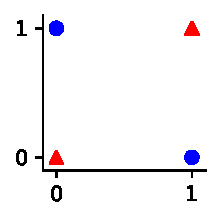
\includegraphics{figures/chapter1/xor_function.pdf}
  \caption{Graphical representation of the XOR function. This function cannot be separated by a linear classifier.}
  \label{figure:xor_function}
\end{figure}
To circumvent these limitations, \citet{minsky1969perceptrons} considered that \emph{another layer of logic} could be added to the function allowing the classification to be done on another representation (see Figure~\ref{figure:multi_layer_perceptron}).
Let $\phi_1$ and $\phi_2$ be two linear functions, we could define a \emph{Multi-Layer Perceptron} as follows:
\begin{equation}
  f(\xvec) = \rho \circ \phi_2 \circ \rho \circ \phi_1( \xvec )
\end{equation}

\begin{figure}[ht]
  \centering
  \begin{subfigure}[t]{0.30\textwidth}
    \centering
    \begin{tabular}{c|c}
      \multicolumn{2}{c}{$\xvec$} \\
      \midrule
      0 & 0 \\
      0 & 1 \\
      1 & 0 \\
      1 & 1
    \end{tabular} 
    \caption*{Input representation}
  \end{subfigure}
  \begin{subfigure}[t]{0.03\textwidth}
    $\rightarrow$
  \end{subfigure}
  \begin{subfigure}[t]{0.30\textwidth}
    \centering
    \begin{tabular}{C{0.5cm} | C{0.5cm}}
      \multicolumn{2}{c}{$\rho \circ \phi_1(\xvec)$} \\
      \midrule
      0 & 0 \\
      0 & 1 \\
      1 & 0 \\
      0 & 0
    \end{tabular}
    \caption*{Intermediate representation}
  \end{subfigure}
  \begin{subfigure}[t]{0.03\textwidth}
    $\rightarrow$
  \end{subfigure}
  \begin{subfigure}[t]{0.30\textwidth}
    \centering
    \begin{tabular}{c}
      $f(\xvec)$ \\
      \midrule
      0 \\
      1 \\
      1 \\
      0
    \end{tabular}
    \caption*{Final representation}
  \end{subfigure}
  \caption{Classification of the XOR function with a Multi-Layer Perceptron}
  \label{figure:multi_layer_perceptron}
\end{figure}

One of the first \emph{Multi-Layer Perceptron}, or now more commonly known as \emph{Deep Neural Network}, was introduced by~\citeauthor{ivakhnenko1967cybernetics} in~\citeyear{ivakhnenko1967cybernetics}.
More precisely, a Neural Neural can be analytically described as a composition of linear functions interlaced with non-linear functions (also called activation functions):
\begin{equation}
  f_\Theta(\xvec) = \phi_{\Wmat_p} \circ \rho \circ \phi_{\Wmat_{p-1}} \circ \cdots \circ \phi_{\Wmat_2} \circ \rho \circ \phi_{\Wmat_1}(\xvec)
  \label{equation:neural_network}
\end{equation}
where the function $\phi_{\Wmat_i}$ is a linear function parameterized by $\Wmat_i$, $\rho$ is a non-linear function, $\Theta \triangleq ( \Wmat_1, \dots, \Wmat_p )$ and $p$ correspond to the \emph{depth} of the network (\ie, the number of layers).
If the weight matrices are dense, this architecture is called \emph{Fully Connected Neural Network} because all the neurons from the first activation are connected to all the neurons from the second activation.

Therefore, a neural network is a function $f_\Theta:\Rbb^n \rightarrow \Rbb^m$ parameterized by weights and composed of at least two linear functions (layers) and one non-linear function (activation function).
The input space $n$ is usually large and the output space $m$ corresponds to the number of classes the network has to classify; therefore, we have $m \ll n$.
In the supervised learning framework, the hypothesis space becomes the set of neural networks parameterized by $\Theta$: $\mathcal{H} = \left\{ f_\Theta \ |\ \Theta = ( \Wmat_1, \dots, \Wmat_p ) \right\}$,
% \begin{equation}
%   \mathcal{H} = \left\{ f_\Theta \ |\ \Theta = \{ \Wmat_1, \dots, \Wmat_p \} \right\} ,
% \end{equation}
then the learning procedure can be taken over $\Theta$ as follows:
\begin{equation}
  \hat{f}^* = \argmin_{\Theta} E(f_\Theta, n) 
\end{equation}



% If $f:\Rbb^n \rightarrow \Rbb^m$ is a two layers neural network:
% \begin{equation}
%   f(\xvec) = \Wmat_2 \rho(\Wmat_1 \xvec)
%   \label{equation:two_layer_neural_network}
% \end{equation}
% where $\Wmat_1 \in \Rbb^{n \times n}$, $\Wmat_2 \in \Rbb^{m \times n}$ are dense matrices.
% This architecture is called \emph{Fully Connected Neural Network} because all the neurons from the first activation are connected to all the neurons from the second activation.

% This type of network can have a large number of parameters, 



%%%%%%%%%%%%%%%%%%%%%%%%%%%%%%%%%%%%%%%%%%%%%%%%%%%%%%%%%%%%%%%%%%%%%%%%%%%%%%%
\section{Introducing Structure into Deep Neural Networks}
\label{section:ch1-introducting_structure_into_deep_neural_networks}
%%%%%%%%%%%%%%%%%%%%%%%%%%%%%%%%%%%%%%%%%%%%%%%%%%%%%%%%%%%%%%%%%%%%%%%%%%%%%%%


Fully connected neural networks can have a very large number of parameters with respect to the number of data points used in real-world datasets.
For example, with the MNIST dataset~\cite{lecun1998gradient} which consists of $5 \times 10^4$ images of handwritten digits from 0 to 9, a two-layer fully connected neural network will have more than $6 \times 10^5$ parameters.
Training such a large network has a number of significant drawbacks: they are hard to train, subject to overfitting and are computationally expensive.
To overcome these limitations, \citet{vapnik1992principles} have proposed to replace the empirical risk minimization principle by \emph{structural risk minimization} (SRM) which consists of implementing ERM with the addition of a structure on the hypothesis space.
Adding a structure on the hypothesis space can be done using two methods: constraining the architecture of the network, constraining the learning procedure by adding a regularization term. 
Hereafter, we present in more detail the two approaches.  

% \begin{itemize}
%   \item reducing the number of parameters by introducing structure into the architecture;
%   \item constraining the learning procedure by adding a regularization term.
% \end{itemize}


% In recent years, Deep Neural Networks have achieved state-of-the-art performances in a variety of domains such as image recognition~\cite{lecun1998gradient,krizhevsky2012imagenet,He_2016_CVPR,tan2019efficientnet}, object detection~\cite{redmon2016you}, natural language processing~\cite{radford2018Language, xxx}, speech recognition~\cite{hinton2012deep, xxx}, etc. 
% This success is mostly due to the advent of specific architectures and learning procedure devised for each applications.  

% However, in order for Deep Neural Networks to achieve such performance, specific architectures and learning procedure have been devised for each application. 
% % More precisely, each of these architectures relies on specific \emph{structured linear transformations}.
%
% In this setting, a phenomenon called overfitting can arise. 
%
% To overcome these limitations,
%
% have proposed two methods to overcome these limitations. 



% \paragraph{Structural Risk Minimization} (SRM).
% The ERM principle assumes that the function $\hat{h}^*$ minimizing $E(h, n)$ leads to the risk $R(\hat{h}^*)$ being close to the minimum.
% This assumption mean that as the \emph{size} of the training set increase the minimization becomes more accurate. More formally, the ERM principle assumes that $R(\hat{h}^*)$ converge to its minimum value on the set $h \in \mathcal{H}$ when $n \rightarrow \infty$.  
% \citet{Vapnik1991TheNA} have shown that this equivalent to say that the empirical risk $E(h, n)$ \emph{converge uniformly} to the actual risk $R(h)$ over $h \in \mathcal{H}$ where the \emph{uniform convergence} is defined as follows:
% \begin{equation}
%   \Pbb \left[ \sup_{h \in \mathcal{H}} \left| R(h) - E(h, n) \right| < \epsilon \right] \rightarrow 0 \quad \text{ when } \quad n \rightarrow \infty, \quad \forall \epsilon > 0 
% \end{equation}

%%%%%%%%%%%%%%%%%%%%%%%%%%%%%%%%%%%%%%%%%%%%%%%%%%%%%%%%%%%%%%%%%%%%%%%%%%%%%%%
\subsection{Structure Given by the Architecture of the Neural Network}
\label{subsection:ch1-introducing_structured_into_the_architecture_of_neural_networks}
%%%%%%%%%%%%%%%%%%%%%%%%%%%%%%%%%%%%%%%%%%%%%%%%%%%%%%%%%%%%%%%%%%%%%%%%%%%%%%%

% In recent years, Deep Neural Networks have achivied state-of-the-art results on computer vision tasks 
%
% In recent years, Deep Neural Networks have achieved state-of-the-art performances in a variety of domains such as image recognition (LeCun et al. 1998; Krizhevsky, Sutskever et al. 2012; He et al. 2016; Tan & Le, 2019), image detection (Redmon et al. 2016), natural language processing (Radford et al. 2018), speech recognition Hinton et al. (2012), etc. 
%
% In order for Deep Neural Networks to achieve such performance, specific architectures have been devised for each application. More precisely, each of these architectures relies on specific structured linear transformations.

\begin{figure}[htb]
  \centering
  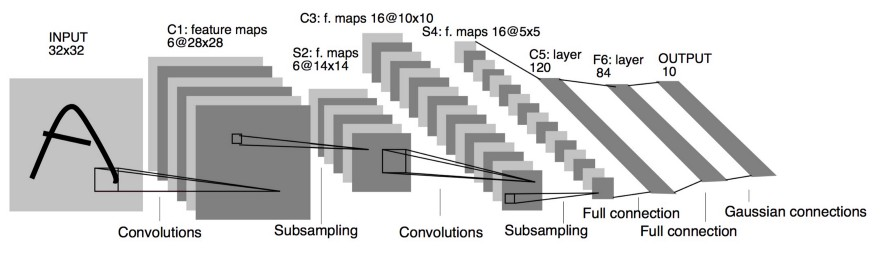
\includegraphics[scale=0.4]{figures/chapter1/lenet.jpg}
  \caption{Graphical representation of the LeNet architecture proposed by \citet{lecun1998gradient}}
  \label{figure:lenet_network}
\end{figure}

A perfect example of neural networks with a specific architecture are \emph{Convolutional Neural Networks} (CNN)~\cite{lecun1998gradient,krizhevsky2012imagenet,He_2016_CVPR,tan2019efficientnet} which consists of neural networks with specific structured linear transformations. 
The structured linear transform used in convolutional layers is the discrete convolution which consists of a kernel sliding over the image and acting as a filter.
% A perfect example of such efficient linear operation is the discrete convolution which consists of a kernel sliding over the image and acting as a filter.
Let $\avec$ and $\bvec$ be two vectors indexed by the set $M = \{-m, -m+1, \dots, m-1, m\}$, the discrete convolution between the signals $\avec$ and $\bvec$ is given by: 
\begin{equation}
  (\avec \ast \bvec) \left[ n \right] \triangleq \sum_{m \in M} \avec\left[m\right] \cdot \bvec\left[n - m\right]
\end{equation}
The convolution operation has translation invariance characteristics \cite{zhang1990parallel} which is perfectly suited for image classification (objects can be at different positions in images).  
\citet{lecun1998gradient} was one of the first to successfully train a convolutional neural network, achieving state-of-the-art performance on the MNIST dataset.
Convolution neural networks achieve such a great result for two main reasons:
first, CNNs are similar to the connectivity pattern of neurons in the visual cortex of the human brain. 
Secondly, CNNs are very efficient due to the sharing of parameters. 
While a classical linear operation with dense matrix has $n \times n$ parameters, a convolution only has $k \times k$ parameters where $k$ is the kernel size and is usually small (\eg 3 or 5 for classical convolution layers use in neural networks).
This weight sharing reduces the number of weights with respect to the fully connected neural network. The LeNet architecture (see Figure~\ref{figure:lenet_network}) has only $6 \times 10^4$ parameters.  


Although, convolutional neural networks perform well on specific tasks, important questions remain on the architecture of neural networks. 
% Which structure is better suited for neural networks?
Can we use other types of structure for neural networks?  
Does the reduction of parameters reduce the performance of the network?


%%%%%%%%%%%%%%%%%%%%%%%%%%%%%%%%%%%%%%%%%%%%%%%%%%%%%%%%%%%%%%%%%%%%%%%%%%%%%%%
\subsection{Structure Given by the Learning Procedure}
\label{subsection:ch1-introducing_structured_into_the_learning_procedure}
%%%%%%%%%%%%%%%%%%%%%%%%%%%%%%%%%%%%%%%%%%%%%%%%%%%%%%%%%%%%%%%%%%%%%%%%%%%%%%%

Instead of constraining the architecture of the network, we can constrain the learning procedure in order to reduce to search space.
Consider the following hypothesis space $\mathcal{H} = \left\{ f_\Theta \ |\ \Theta = ( \Wmat_1, \cdots, \Wmat_p ) \right\}$ which define the set of neural networks with fixed architecture.
We can introduce a structure in the hypothesis space by setting:
\begin{equation}
  \mathcal{H} = \left\{ f_\Theta \ |\ \Theta = ( \Wmat_1, \cdots, \Wmat_p ) \ |\ R(\Theta) \right\} 
\end{equation}
where $R(\Theta)$ is a constrain on $\Theta$ called a regularizer.
One of the most common form of regularization consists of adjusting the weights during the learning procedure under the constraint to keep the magnitude of the weights small.
This regularization has been introduced by~\citet{tikhonov_arsenin_1977} and is commonly known as \emph{weight decay}.
With this constraint, the hypothesis space can be defined as follows:
\begin{equation}
  \mathcal{H_\epsilon} = \left\{ f_\Theta \ |\ \Theta = (\Wmat_1, \cdots, \Wmat_p) \ | \ \norm{\Wmat_i}_\mathrm{F} \leq \epsilon \right\} 
\end{equation}
For a convex loss function, the minimization of the empirical risk within the set $\mathcal{H}_\epsilon$ can be achieved with the minimization of
\begin{equation}
  E(f_\Theta, n, \lambda) = \frac{1}{n} \sum_{i = 1}^{n} L\left(f_\Theta(\xvec^{(i)}), y^{(i)} \right) + \lambda \sum_{i = 1}^{p} \norm{\Wmat_i}_\mathrm{F}
\end{equation}
where $\lambda$ is a Lagrange multiplier.

Defining a regularization strategy is still an open problem in supervised learning. Recent works have proposed different form of regularization.  











%
%
% The concept of \emph{supervised learning} which refers to the notion of learning the parameters of a specific function (neural network) that maps an input to an output based on example input-output pairs.
% For example, an image (input) associated with its content: label (output).
% The steps of the learning procedure are as follows. 
% First, a neural network is initialized with random weights.
% Then, the algorithm \emph{analyzed} the training dataset and \emph{adjust} the weights in order for the network to correctly map the input to the output. 
%
% Due to the important expressivity of neural networks and of the finite number of sample data point, the learning procedure can produce a learned neural network that fits to closely on the training dataset and fail to fit on unseen example.
% This phenomenon is called \emph{overfitting} and can significantly decrease the general performance of neural networks.
% In order to limit overfitting and improve the general performance of neural network, \citet{vapnik1992principles} have proposed to constraint the learning procedure by adding a regularization term.  



% Another method proposed by \cite{vapnik1992principles} is to constraint the learning procedure in order to improve the performance of neural networks. 
%
% Important questions remain on supervised learning algorithms:
% Which properties can we leverage from these structures to improve the training and performance of neural networks? 


% Overfitting is a modeling error that occurs when a function is too closely fit to a limited set of data points. Overfitting the model generally takes the form of making an overly complex model to explain idiosyncrasies in the data under study.


% The choice of the function used for supervised learning is an active area of research and will be part of the focus of this thesis.
% In this work, we study \emph{neural networks} which are a class of function widely used for unstructured datasets (image, sound, text).






%%%%%%%%%%%%%%%%%%%%%%%%%%%%%%%%%%%%%%%%%%%%%%%%%%%%%%%%%%%%%%%%%%%%%%%%%%%%%%%
\section{Main contributions and Outline of the Thesis}
\label{section:ch1-main_contributions_and_outline_of_the_thesis}
%%%%%%%%%%%%%%%%%%%%%%%%%%%%%%%%%%%%%%%%%%%%%%%%%%%%%%%%%%%%%%%%%%%%%%%%%%%%%%%

%%%%%%%%%%%%%%%%%%%%%%%%%%%%%%%%%%%%%%%%%%%%%%%%%%%%%%%%%%%%%%%%%%%%%%%%%%%%%%%
\subsection{Main Contributions}
\label{subsection:ch1-main_contributions}
%%%%%%%%%%%%%%%%%%%%%%%%%%%%%%%%%%%%%%%%%%%%%%%%%%%%%%%%%%%%%%%%%%%%%%%%%%%%%%%

In this thesis, we leverage the properties of \emph{structured matrices} for the problems mentioned in Section~\ref{subsection:ch1-introducing_structured_into_the_architecture_of_neural_networks} and \ref{subsection:ch1-introducing_structured_into_the_learning_procedure}. A $n \times n$ structure matrix can be represented with less than $n^2$ parameters, Figure~\ref{figure:example_structure_matrices} shows an example of structured matrices.
In addition to offering a more compact representation, the structure of certain matrices can be leveraged to obtain better algorithms for matrix-vector product leading in memory and computationally operations. 

\begin{figure}[ht]
   \centering
   \begin{subfigure}[t]{0.24\textwidth}
       \centering
       \begin{equation*}
	  \leftmatrix
	    a &   &   &   \\
	      & b &   &   \\
	      &   & c &   \\
	      &   &   & d
	  \rightmatrix
       \end{equation*}
       \caption*{diagonal}
   \end{subfigure}
   \hfill
   \begin{subfigure}[t]{0.24\textwidth}
       \centering
       \begin{equation*}
	  \leftmatrix
	    a & b & c & d \\
	    e & a & b & c \\
	    f & e & a & b \\
	    d & f & e & a
	  \rightmatrix
       \end{equation*}
       \caption*{Toeplitz}
   \end{subfigure}
   \hfill
   \begin{subfigure}[t]{0.24\textwidth}
       \centering
       \begin{equation*}
	  \leftmatrix
	    ae & af & ag & ah \\
	    be & bf & bg & bh \\
	    ce & cf & cg & ch \\
	    de & df & dg & dh
	  \rightmatrix
       \end{equation*}
       \caption*{Low Rank}
   \end{subfigure}
   \hfill
   \begin{subfigure}[t]{0.24\textwidth}
       \centering
       \begin{equation*}
	  \leftmatrix
	    a & a^2 & a^3 & a^4 \\
	    b & b^2 & b^3 & b^4 \\
	    c & c^2 & c^3 & c^4 \\
	    d & d^2 & d^3 & d^4
	  \rightmatrix
       \end{equation*}
       \caption*{Vandermonde}
   \end{subfigure}
  \caption{Examples of structured matrices.}
  \label{figure:example_structure_matrices}
\end{figure}

More specifically, we study the proprieties of structured matrices from the Toeplitz family to make two contributions presented below:

\paragraph{Contribution 1} (C1)
We use circulant matrices, which are a particular case of Toeplitz matrices, to devise a new compact architecture replacing Fully Connected Neural Networks.
More precisely, we study deep diagonal circulant neural networks, which are deep neural networks in which weight matrices are the product of diagonal and circulant ones.
Besides making a theoretical analysis of their expressivity, we introduce principled techniques for training these models: we devise an initialization scheme and propose a smart use of non-linearity functions in order to train deep diagonal circulant networks. 
Furthermore, we show that these networks outperform recently introduced deep networks with other types of structured layers.
We conduct a thorough experimental study to compare the performance of deep diagonal circulant networks with state-of-the-art models based on structured matrices and with dense models.
We show that our models achieve better accuracy than other structured approaches while requiring 2x fewer weights than the next best approach.
Finally, we train compact and accurate deep diagonal circulant networks on a real-world video classification dataset with over 3.8 million training examples. 

\paragraph{Contribution 2} (C2)
It is well known that a discrete convolution operation with a 2d kernel applied on a 2d signal is equivalent to a matrix multiplication with a doubly-block Toeplitz matrix~\cite{jain1989fundamentals} (see Appendix~\ref{xxx}). 
Based on this knowledge and by leveraging the theory of Toeplitz matrices, we introduce a new upper bound on the Lipschitz constant for convolutional layers that is both tight and easy to compute.
This bound allows us to tackle the problem of Lipschitz regularization of Convolutional Neural Networks which is established now established as a key property of modern deep learning with implications in training stability, generalization, robustness against adversarial examples, etc.

% we leverage the properties of doubly-block Toeplitz matrices to devised a new fast and efficient method to compute the Lipschitz constant of convolutional layers. 
%
% However, computing the exact value of the Lipschitz constant of a neural network is known to be NP-hard.
% Recent attempts from the literature introduce upper bounds to approximate this constant that are either efficient but loose or accurate but computationally expensive.
% In this work, Based on this result we devise an algorithm to train Lipschitz regularized Convolutional Neural Networks.
%
% The contributions of this Thesis are based on structured matrices from the Toeplitz family.
%
% More specifically, in Chapter~\ref{chapter:diagonal_circulant_neural_network}, In Chapter~\ref{chapter:lipschitz_bound}, we leverage the structure of convolutional layers to devise a new regularization scheme for neural networks. 


%%%%%%%%%%%%%%%%%%%%%%%%%%%%%%%%%%%%%%%%%%%%%%%%%%%%%%%%%%%%%%%%%%%%%%%%%%%%%%%
\subsection{Outline of the Thesis}
\label{subsection:ch1-outline_of_the_thesis}
%%%%%%%%%%%%%%%%%%%%%%%%%%%%%%%%%%%%%%%%%%%%%%%%%%%%%%%%%%%%%%%%%%%%%%%%%%%%%%%

\todo{update this paragraph at the end of the writing}

% The thesis is organized as follows. The first Chapter (Chapter~\ref{chapter:related_work}) is dedicated to enumerating state-of-the-art approaches on both contributions. In a first part, we review approaches on compact neural networks. In a second part, we review  
%
% Chapter~\ref{chapter:related_work} present a related work in two parts: first we review existing techniques for on building compact neural network architecture. Then, we present different techniques to constraint the learning procedure. 
%
% The following two chapters contains the main contributions of the Thesis.  
% Finally, Chapter~\ref{chapter:conclusion} provides concluding remarks and a discussion.



  %%%%%%%%%%%%%%%%%%%%%%%%%%%%%%%%%%%%%%%%%%%%%%%%%%%%%%%%%%%%%%%%%%%%%%%%
\chapter{Background}
\label{chapter:background}
%%%%%%%%%%%%%%%%%%%%%%%%%%%%%%%%%%%%%%%%%%%%%%%%%%%%%%%%%%%%%%%%%%%%%%%%
\localtableofcontents

%%%%%%%%%%%%%%%%%%%%%%%%%%%%%%%%%%%%%%%%%%%%%%%%%%%%%%%%%%%%%%%%%%%%%%%%%%%%%%%
\section{Supervised Learning \& Neural Networks}
\label{secction:ch2-supervised_learning_neural_networks}
%%%%%%%%%%%%%%%%%%%%%%%%%%%%%%%%%%%%%%%%%%%%%%%%%%%%%%%%%%%%%%%%%%%%%%%%%%%%%%%

This thesis focus on the concept of \emph{supervised learning} which refers to the notion of learning the parameters of a specific function that maps an input to an output based on example input-output pairs.
For example, an image (input) associated with its content: label (output).
The choice of the function used for supervised learning is an active area of research and will be part of the focus of this thesis.
In this work, we study \emph{neural networks} which are a class of function widely used for unstructured datasets (image, sound, text).

%%%%%%%%%%%%%%%%%%%%%%%%%%%%%%%%%%%%%%%%%%%%%%%%%%%%%%%%%%%%%%%%%%%%%%%%%%%%%%%
\subsection{Supervised Learning}
\label{subsection:ch2-supervised_learning}
%%%%%%%%%%%%%%%%%%%%%%%%%%%%%%%%%%%%%%%%%%%%%%%%%%%%%%%%%%%%%%%%%%%%%%%%%%%%%%%

Let us consider an input space $\mathcal{X} = [0, 1]^d$ of dimension $d$, an output space $\mathcal{Y} = [k]$ where $k$ is the number of class and a data distribution $\mathcal{D}$ over $\mathcal{X} \times \mathcal{Y}$.
We seek to find a function $h: \mathcal{X} \rightarrow \mathcal{Y}$ that maps the input $\xvec \in \mathcal{X}$ to the output $y \in \mathcal{Y}$ with $h \in \mathcal{H}$ where $h$ is called the \emph{hypothesis} and $\mathcal{H}$ the \emph{hypothesis space}.
In order to measure how well the function fits, a \emph{loss function} $L: \mathcal{Y} \times \mathcal{Y} \rightarrow \Rbb^{+}$ is defined.
The \emph{risk} $R$ associated with the hypothesis $h(\xvec)$ is defined as follows:
\begin{equation}
  R(h) \triangleq \Ebb_{(\xvec, y) \sim \mathcal{D}}\  L \left( h(\xvec), y \right)
\end{equation}
The 0-1 loss function is a natural loss function to use because it assigns 0 for a correct classification and 1 for an incorrect classification. 
The goal of a \emph{learning algorithm} is to find an hypothesis $h^* \in \mathcal{H}$ which minimize the risk $R(h)$:
\begin{equation}
  h^* \triangleq \argmin_{h \in \mathcal{H}} R(h) .
\end{equation}


\paragraph{Empirical Risk Minimization} (ERM).
In practice, the joint probability distribution $\mathcal{D}$ is unknown.
Instead, we have $n$ independent observations of the distribution called the \emph{training set}
\begin{equation}
  \left\{ (\xvec^{(1)}, y^{(1)}), \dots, (\xvec^{(n)}, y^{(n)}) \right\} ,
\end{equation}
where $\xvec \in \mathcal{X}$ and $y \in \mathcal{Y}$.
The risk minimization problem is therefore replace by the \emph{empirical risk minimization} as follows:
\begin{equation}
  E(h, n) \triangleq \frac{1}{n} \sum_{i = 0}^{n} L\left(h\left(\xvec^{(i)}\right), y^{(i)}\right) ,
\end{equation}
the learning algorithm then becomes:
\begin{equation}
  \hat{h}^* \triangleq \argmin_{h \in \mathcal{H}} E(h, n)  .
\end{equation}


\paragraph{Structural Risk Minimization} (SRM).
The ERM principle assumes that the function $\hat{h}^*$ minimizing $E(h, n)$ leads to the risk $R(\hat{h}^*)$ being close to the minimum.
However, does increasing the \emph{size} of the training set allow a better minimisation of the actual risk. More formally, does $R(\hat{h}^*)$ converge to its minimum value on the set $h \in \mathcal{H}$ when $n \rightarrow \infty$. 
\citet{Vapnik1991TheNA} have shown that this question is equivalent to the following: does the empirical risk $E(h, n)$ \emph{converge uniformly} to the actual risk $R(h)$ over $h \in \mathcal{H}$ where the \emph{uniform convergence} is defined as follows:
\begin{equation}
  \Pbb \left[ \sup_{h \in \mathcal{H}} \left| R(h) - E(h, n) \right| < \epsilon \right] \rightarrow 0 \quad \text{ when } \quad n \rightarrow \infty, \quad \forall \epsilon > 0 
\end{equation}


\citet{vapnik1992principles} 


\begin{enumerate}
  \item Structure given by the architecture of the neural network: xxx
  \item Structure given by the learning procedure: xxx 
\end{enumerate}








%
% of the ERM principle \ie, does $R(\hat{h}^*)$ converge to its minimum value on the set $h \in \mathcal{H}$ when $n \rightarrow \infty$ is equivalent to the question: 
%
% is equivalent to the question: does the empirical risk E(h, n) \emph{converge uniformly} to the actual risk $R(h)$ over $h \in \mat
%
% An interesting question to ask is 


% \begin{equation}
%   h^* = \argmin_{h \in \mathcal{H}} \frac{1}{n} \sum_{i = 0}^{n} L(h(\xvec_i), y) + \lambda C(\theta) 
% \end{equation}


% Because the relation between $\xvec \in \mathcal{X}$ and $y \in \mathcal{Y}$ is unknown, we aim to find the best approximation of the function $h$ with a parameterized function $h_\theta \in \mathcal{H}$ where $\mathcal{H}$ is called the \emph{hypothesis space}.


% The goal of a \textbf{learning algorithm} is to learn a function $f: \mathcal{X} \rightarrow \mathcal{Y}$ which outputs $y \in \mathcal{Y}$ given an input $\xvec \in \mathcal{X}$ with $f \in \mathcal{H}$ where $\mathcal{H}$ is called the \emph{hypothesis space}.
%
% The supervised learning settings assume that a function $f: \mathcal{X} \rightarrow \mathcal{Y}$ exists. 
%
% The supervised learning settings assume that a function $f$ that maps $\xvec \sim \mathcal{X}$ to $y \sim \mathcal{y}$ exists. 



% The goal of a \textbf{learning algorithm} is to approximate $f$ by a parameterized function $f_\theta$.
% The standard method to learn the set of parameters $\theta$ is the \textbf{empirical risk minimization (ERM)}:
% \begin{equation*}
%   \hat{\theta}_{ERM} \triangleq \argmin_{\theta} \frac{1}{n} \sum_{i=1}^{n} L (f_{\theta} (\xvec_i), y_i )
% \end{equation*}

% \begin{equation}
%   \min_{\theta} \Ebb_{(\xvec, y) \sim \mathcal{D}} \left[ L(f_\theta(x), y) \right]. 
% \end{equation}





%%%%%%%%%%%%%%%%%%%%%%%%%%%%%%%%%%%%%%%%%%%%%%%%%%%%%%%%%%%%%%%%%%%%%%%%%%%%%%%
\subsection{Neural Networks}
\label{subsection:ch2-neural_networks}
%%%%%%%%%%%%%%%%%%%%%%%%%%%%%%%%%%%%%%%%%%%%%%%%%%%%%%%%%%%%%%%%%%%%%%%%%%%%%%%
xxx


%%%%%%%%%%%%%%%%%%%%%%%%%%%%%%%%%%%%%%%%%%%%%%%%%%%%%%%%%%%%%%%%%%%%%%%%%%%%%%%
\subsection{Evaluation of Neural Networks}
\label{subsection:ch2-evaluation_neural_networks}
%%%%%%%%%%%%%%%%%%%%%%%%%%%%%%%%%%%%%%%%%%%%%%%%%%%%%%%%%%%%%%%%%%%%%%%%%%%%%%%
xxx

%%%%%%%%%%%%%%%%%%%%%%%%%%%%%%%%%%%%%%%%%%%%%%%%%%%%%%%%%%%%%%%%%%%%%%%%%%%%%%%
\subsubsection{Classical Evaluation of Neural Networks}
\label{section:ch2-preliminaries_adversarial_attacks_and_defenses}
%%%%%%%%%%%%%%%%%%%%%%%%%%%%%%%%%%%%%%%%%%%%%%%%%%%%%%%%%%%%%%%%%%%%%%%%%%%%%%%
xxx

%%%%%%%%%%%%%%%%%%%%%%%%%%%%%%%%%%%%%%%%%%%%%%%%%%%%%%%%%%%%%%%%%%%%%%%%%%%%%%%
\subsubsection{Preliminaries on Adversarial Attacks and Defenses}
\label{section:ch2-preliminaries_adversarial_attacks_and_defenses}
%%%%%%%%%%%%%%%%%%%%%%%%%%%%%%%%%%%%%%%%%%%%%%%%%%%%%%%%%%%%%%%%%%%%%%%%%%%%%%%

Deep neural networks achieve state-of-the-art performances in a variety of domains such as natural language processing~\cite{radford2018Language}, image recognition~\cite{He_2016_CVPR} and speech recognition~\cite{hinton2012deep}.
However, it has been shown that such neural networks are vulnerable to \emph{adversarial examples}, \ie, imperceptible variations of the natural examples, crafted to deliberately mislead the models~\cite{globerson2006nightmare,biggio2013evasion,Szegedy2013IntriguingPO}.
Since their discovery, a variety of algorithms have been developed to generate adversarial examples (\aka attacks), for example FGSM \cite{goodfellow2014explaining}, PGD \cite{madry2018towards} and C\&W \cite{carlini2017towards}, to mention the most popular ones.

Because it is difficult to characterize the space of visually imperceptible variations of a natural image, existing adversarial attacks use surrogates that can differ from one attack to another.
For example, \citet{goodfellow2014explaining} use the $\linf$ norm to measure the distance between the original image and the adversarial image whereas \citet{carlini2017towards} use the $\ltwo$ norm.
When the input dimension is low, the choice of the norm is of little importance because the $\linf$ and $\ltwo$ balls overlap by a large margin, and the adversarial examples lie in the same space.
An important insight in this paper is to observe that the overlap between the two balls  diminishes exponentially quickly as the dimensionality of the input space increases.
For typical image datasets with large dimensionality, the two balls are mostly disjoint.
As a consequence, the $\linf$ and the $\ltwo$ adversarial examples lie in different areas of the space, and it explains why $\linf$ defense mechanisms perform poorly against $\ltwo$ attacks and vice versa. 

% Building on this insight, we advocate for designing models that incorporate defense mechanisms against both $\linf$ and $\ltwo$ attacks and review several ways of mixing existing defense mechanisms.
% In particular, we evaluate the performance of  {\em Mixed Adversarial Training} (MAT)~\cite{goodfellow2014explaining} which consists of  augmenting training batches using \emph{both} $\linf$ and $\ltwo$ adversarial examples, and {\em Randomized Adversarial Training} (RAT)~\cite{salman2019provably}, a solution to benefit from the advantages of both $\linf$ adversarial training, and $\ltwo$ randomized defense. 


Let us first consider a standard classification task with an input space $\mathcal{X}=[0,1]^d$ of dimension $d$,  an output space $\mathcal{Y}=[K]$ and a data distribution $\mathcal D$ over $\mathcal X \times \mathcal Y$.
We assume the model $f_\theta$ has been trained to minimize the expectation over $\mathcal{D}$ of a loss function $L$ as follows:
\begin{equation}
  \min_{\theta} \Ebb_{(\xvec, y) \sim \mathcal{D}} \left[ L(f_\theta(\xvec), y) \right]. 
  \label{equation:ch2-classification}
\end{equation}

%%%%%%%%%%%%%%%%%%%%%%%%%%%%%%%%%%%%%%%%%%%%%%%%%%%%%%%%%%%%%%%%%%%%%%%%%%%%%%%
\subsection{Adversarial attacks}
\label{subsection:ch2-adversarial_attacks}
%%%%%%%%%%%%%%%%%%%%%%%%%%%%%%%%%%%%%%%%%%%%%%%%%%%%%%%%%%%%%%%%%%%%%%%%%%%%%%%
 
Given an input-output pair $(\xvec, y) \sim \mathcal{D}$, an \emph{adversarial attack} is a procedure that produces a small perturbation $\pmb{\tau} \in  \mathcal X$  such that $f_\theta(\xvec + \pmb{\tau}) \neq y$.
To find the best perturbation $\pmb{\tau}$, existing attacks can adopt one of the two following strategies:
\begin{itemize}
  \item[(I)] \textbf{Loss maximization}: maximizing the loss $\mathcal L(f_\theta(\xvec + \pmb{\tau}), y)$ under some constraint on $\norm{\pmb{\tau}}_p$ with $p \in \{0, \cdots, \infty\}$.;
  \item[(II)] \textbf{Perturbation minimization}: minimizing $\norm{\pmb{\tau}}_p$ under some constraint on the loss $L(f_\theta(\xvec + \pmb{\tau}), y)$.
\end{itemize}

\paragraph{(i) Loss maximization.}
In this scenario, the procedure maximizes the loss objective function, under the constraint that the $\lp$ norm of the perturbation remains bounded by some value $\epsilon$, as follows:  

\begin{equation}
  \argmax_{\norm{\pmb{\tau}}_p \leq \epsilon} L(f_\theta(\xvec + \pmb{\tau}),y).
  \label{equation:ch2-lossmax}
\end{equation}

The typical value of $\epsilon$ depends on the norm $\norm{\cdot}_p$ considered in the problem setting.
In order to compare $\linf$ and $\ltwo$ attacks of similar strength, we choose values of $\epsilon_\infty$ and $\epsilon_2$ (for $\linf$ and $\ltwo$ norms respectively) which result in $\linf$ and $\ltwo$ balls of equivalent volumes.
For the particular case of CIFAR-10, this would lead us to choose $\epsilon_\infty = 0.03$ and $\epsilon_2 = 0.8$ which correspond to the maximum values chosen empirically to avoid the generation of visually detectable perturbations. 
The current state-of-the-art method to solve Problem~(\ref{equation:ch2-lossmax}) is based on a projected gradient descent (PGD)~\cite{madry2018towards} of radius~$\epsilon$. Given a budget $\epsilon$, it recursively computes
\begin{equation}
    \xvec^{t+1}=\prod_{B_p(\xvec,\epsilon)}\left(\xvec^t
    +\alpha \argmax_{\delta \text{ s.t. } \norm{\delta}_p \leq 1} \left( \Delta^t \ |\ \delta \right)\right)
    \label{equation:ch2-projectionPGD}
\end{equation}
where $B_p(\xvec,\epsilon) = \{ \xvec + \pmb{\tau} \text{ s.t. } \norm{\pmb{\tau}}_p \leq \epsilon\}$, $\Delta^t = \nabla_\xvec L\left( f_\theta \left(\xvec^t \right), y \right)$, $\alpha$ is a gradient step size, and $\prod_S$ is the projection operator on $S$. Both PGD attacks with $p=2$, and $p=\infty$ are currently used in the literature as state-of-the-art attacks for the loss maximization problem. 


\paragraph{(ii) Perturbation minimization.}
This type of procedure search for the perturbation that has the minimal $\lp$ norm, under the constraint that $L(f_\theta(\xvec + \pmb{\tau}), y)$ is bigger than a given bound $c$:
\begin{equation}
  \argmin_{L(f_\theta(\xvec + \pmb{\tau}), y) \geq c} \norm{\pmb{\tau}}_p.
  \label{equation:ch2-normmin}
\end{equation}
The value of $c$ is typically chosen depending on the loss function $L$. For example, if $L$ is the $0/1$ loss, any $c > 0$ is acceptable.
Problem~\ref{equation:ch2-normmin} has been tackled by~\citep{carlini2017towards}, leading to the following method, denoted C\&W attack in the rest of the chapter. It aims at solving the following Lagrangian relaxation of Problem~\ref{equation:ch2-normmin}:
\begin{equation}
  \argmin_{\pmb{\tau}} \norm{\pmb{\tau}}_p+ \lambda \times g(x+\pmb{\tau})
  \label{equation:ch2-CWproblem}
\end{equation}
where $g(x+\pmb{\tau})<0$ if and only if $L(f_\theta(x+\pmb{\tau}),y) \geq c$. 
The authors use a change of variable $\pmb{\tau}=\tanh(w)-x$ to ensure that $-1 \leq x+\pmb{\tau} \leq 1$, a binary search to optimize the constant $c$, and Adam or SGD to compute an approximated solution.
The C\&W attack is well defined both for $p=2$, and $p=\infty$, but there is a clear empirical gap of efficiency in favor of the $\ltwo$ attack.

In this paper, we focus on the \emph{Loss Maximization} setting using the PGD attack. However we conduct some of our experiments using \emph{Perturbation Minimization} algorithms such as C\&W to capture more detailed information about the location of adversarial examples in the vector space\footnote{As it has a more flexible geometry than the \emph{Loss Maximization} attacks.}. 

%%%%%%%%%%%%%%%%%%%%%%%%%%%%%%%%%%%%%%%%%%%%%%%%%%%%%%%%%%%%%%%%%%%%%%%%%%%%%%%
\subsection{Defense mechanisms}
\label{subsection:ch2-defense_mechanisms}
%%%%%%%%%%%%%%%%%%%%%%%%%%%%%%%%%%%%%%%%%%%%%%%%%%%%%%%%%%%%%%%%%%%%%%%%%%%%%%%

\paragraph{Adversarial Training (AT).}
Adversarial Training was introduced by \citep{goodfellow2014explaining} and later improved by \citep{madry2018towards} as a first defense mechanism to train robust neural networks.
It consists in augmenting training batches with adversarial examples generated during the training procedure.
The standard training procedure from Equation~\ref{equation:ch2-classification} is thus replaced by the following  $\min$ $\max$ problem, where the classifier tries to minimize the expected loss under maximum perturbation of its input:
\begin{equation}
  \min_{\theta} \Ebb_{(\xvec, y) \sim \mathcal{D}} \left[ \max_{\norm{\pmb{\tau}}_p \leq \epsilon} L \left( f_{\theta}(\xvec + \pmb{\tau}), y \right) \right].
\end{equation}

In the case where $p=\infty$, this technique offers good robustness  against $\linf$ attacks \cite{athalye2018obfuscated}. AT can also be used with $\ltwo$ attacks but as we will discuss in Section~\ref{section:ch2-no_free_lunch}, AT with one norm offers poor protection against the other.
The main weakness of Adversarial Training is its lack of formal guarantees.
Despite some recent work providing great insights \cite{sinha2017certifying,zhang2019theoretically}, there is no worst case lower bound yet on the accuracy under attack of this method.


\paragraph{Noise injection mechanisms (NI).}
\label{subsection:ch2-randomized_training}

Another important technique to defend against adversarial examples is to use Noise Injection. 
In contrast with Adversarial Training, Noise Injection mechanisms are usually deployed after training.
In a nutshell, it works as follows.
At inference time, given a unlabeled sample $x$, the network outputs
\begin{equation}
  \tilde{f}_\theta(\xvec) \triangleq f_\theta(\xvec + \eta) \ \ \ (\text{instead of  } f_\theta(\xvec)) 
\end{equation}
where $\eta$ is a random variable on $\mathbb{R}^d$.
Even though, Noise Injection is often less efficient than Adversarial Training in practice (see \eg, Table~\ref{table:ch2-results}), it benefits from strong theoretical background.
In particular, recent works \cite{lecuyer2018certified,NIPS2019_9143}, followed by \cite{KolterRandomizedSmoothing,pinot2019theoretical} demonstrated that noise injection from a Gaussian distribution can give provable defense against $\ltwo$ adversarial attacks.
In this work, besides the classical Gaussian noises already investigated in previous works, we evaluate the efficiency of Uniform distributions to defend against $\ltwo$ adversarial examples. 


% \citeauthor{werbos1974thesis,rumelhart1986learning} conside
%
% While connectionism approaches were abandoned for the next few years, Paul Werbos revived the field with the discovery of the \emph{backpropagation} algorithm \cite{werbos1974thesis} which as been popularized later on by \citet{rumelhart1986learning}.
%
% During the training of the neural network, the backpropagation algorithm \emph{efficiently} computes the gradient of the loss function we seek to minimize allowing the training of multi layer neural network. In practice, the backpropagation algorithm is simply an application of the chain rule for the composition of function. If $h$, $f$ and $g$ are differentiable functions and $h(x) = (f \circ g)(x)$ then:
% \begin{equation}
%   h'(x) = (f \circ g)' = (f' \circ g) \cdot g'.
% \end{equation}

% This discovery led to the first large scale application with the US Post Office. Yann Lecun successfully devise a Convolutional Neural Network to recognize hand written digits \cite{lecun1998gradient}.



% \section{From Neural Networks to Deep Learning}
%
% Neural Networks find they roots, in 1958, in the works of Frank Rosenblatt \cite{rosenblatt1958perceptron} where for the first time, the Perceptron, an electronic device inspired by the human brain, showed ability to \emph{learn} from multiples examples.
% This work had greatly advanced the concepts of connectionism \cite{medler1998brief} and was described as revolutionary by the New York Times \todo{cite} \cite{}. 
%
%
% \todo{detail limit sign(f(x))}
%
% While connectionism approaches were abandoned for the next few years, Paul Werbos revived the field with the discovery of the \emph{backpropagation} algorithm \cite{werbos1974thesis} which as been popularized later on by \citet{rumelhart1986learning}.
%
% During the training of the neural network, the backpropagation algorithm \emph{efficiently} computes the gradient of the loss function we seek to minimize allowing the training of multi layer neural network. In practice, the backpropagation algorithm is simply an application of the chain rule for the composition of function. If $h$, $f$ and $g$ are differentiable functions and $h(x) = (f \circ g)(x)$ then:
% \begin{equation}
%   h'(x) = (f \circ g)' = (f' \circ g) \cdot g'.
% \end{equation}
%
% This discovery led to the first large scale application with the US Post Office. Yann Lecun successfully devise a Convolutional Neural Network to recognize hand written digits \cite{lecun1998gradient}.




%%%%%%%%%%%%%%%%%%%%%%%%%%%%%%%%%%%%%%%%%%%%%%%%%%%%%%%%%%%%%%%%%%%%%%%%%%%%%%%
\section{Primer on Structured Matrices}
\label{secction:ch2-primer_structured_matrices}
%%%%%%%%%%%%%%%%%%%%%%%%%%%%%%%%%%%%%%%%%%%%%%%%%%%%%%%%%%%%%%%%%%%%%%%%%%%%%%%
xxx



%%%%%%%%%%%%%%%%%%%%%%%%%%%%%%%%%%%%%%%%%%%%%%%%%%%%%%%%%%%%%%%%%%%%%%%%%%%%%%%
\subsection{Introduction on Circulant Matrices}
\label{subsection:primer_circulant_matrices}
%%%%%%%%%%%%%%%%%%%%%%%%%%%%%%%%%%%%%%%%%%%%%%%%%%%%%%%%%%%%%%%%%%%%%%%%%%%%%%%

An $n$-by-$n$ circulant matrix $\Cmat$ is a matrix where each row is a cyclic right shift of the previous one as illustrated below.

\begin{equation}
    \Cmat = \circulant(\cvec) = \leftmatrix
    c_{0} & c_{n-1} & c_{n-2} & \dots & c_{1} \\
    c_{1} & c_{0} & c_{n-1} & & c_{2} \\
    c_{2} & c_{1} & c_{0}& & c_{3} \\
    \vdots & & & \ddots & \vdots \\
    c_{n-1} & c_{n-2} & c_{n-3} & & \phantom{0}c_{0}\phantom{0}
    \rightmatrix
\end{equation}

Circulant matrices exhibit several interesting properties from the perspective of numerical computations.
Most importantly, any $n$-by-$n$ circulant matrix $\Cmat$ can be represented using only $n$ coefficients instead of the $n^2$ coefficients required to represent classical unstructured matrices.
In addition, the matrix-vector product is simplified from $O(n^2)$ to $O(n \log n)$ using the  convolution theorem.


%%%%%%%%%%%%%%%%%%%%%%%%%%%%%%%%%%%%%%%%%%%%%%%%%%%%%%%%%%%%%%%%%%%%%%%%%%%%%%%
\subsection{Convolution as Matrix Multiplication}
\label{subsection:convolution_as_matrix_multiplication}
%%%%%%%%%%%%%%%%%%%%%%%%%%%%%%%%%%%%%%%%%%%%%%%%%%%%%%%%%%%%%%%%%%%%%%%%%%%%%%%

A discrete convolution between a signal $\mathbf{x}$ and a kernel $\mathbf{k}$ can be expressed as a  product between the vectorization of $\mathbf{x}$ and a doubly-block Toeplitz matrix $\textbf{M}$, whose coefficients have been chosen to match the convolution $\mathbf{x} * \mathbf{k}$.
For a 2-dimensional signal $\mathbf{x} \in \mathbb{R}^{n \times n}$ and a kernel $\mathbf{k} \in \mathbb{R}^{m \times m}$ with $m$ odd, the convolution operation can be written as follows:
\begin{equation} \label{equation:equation_conv_as_matrix}
    \reshape(\mathbf{y}) = \reshape(\pad(\mathbf{x}) * \mathbf{k}) = \Mmat \reshape(\mathbf{x})
\end{equation}
where $\Mmat$ is a $n^2$-by-$n^2$  doubly-block Toeplitz matrix, \ie a block Toeplitz matrix where the blocks are also Toeplitz (Note that this is not a doubly-block circulant matrix because of the padding.), $\mathbf{y}$ is the output of size $q \times q$ with $q = n - m + 2p + 1$, (see \eg \cite{dumoulin2016guide}).
The $\reshape: \mathbb{R}^{n \times n} \rightarrow \mathbb{R}^{n^2}$ operator is defined as follows: $\reshape(\mathbf{x})_q = \mathbf{x}_{\lfloor q/n \rfloor,\ q\mod n}$.
The $\pad: \mathbb{R}^{n \times n} \rightarrow \mathbb{R}^{(n+2p) \times (n+2p)}$ operator is a zero-padding operation which takes a signal $\mathbf{x}$ of shape $\mathbb{R}^{n \times n}$ and adds $0$ on the edges so as to obtain a new signal $\mathbf{y}$ of shape $\mathbb{R}^{(n+2p) \times (n+2p)}$.
In order to have the same shape between the convoluted signal and the signal, we set $ p = \lfloor m/2 \rfloor$ \footnote{We take a square signal and an odd size square kernel to simplify the notation but the same applies for any input and kernel size.
Also, we take a specific padding in order to have the same size between the input and output signal.
But everything in the paper can be generalized to any paddings.}.

We now present an example of the convolution operation with doubly-block Toeplitz matrix.
Let us define a kernel $\mathbf{k} \in \mathbb{R}^{3\times3}$ as follows:
\begin{equation}
    \mathbf{k} = \begin{pmatrix}
        k_{0} & k_{1} & k_{2} \\
        k_{3} & k_{4} & k_{5} \\
        k_{6} & k_{7} & k_{8} 
    \end{pmatrix}
\end{equation}
If we set the padding to 1, then, the matrix $\Mmat$ is a tridiagonal doubly-block Toeplitz matrix of size $n \times n$ and has the following form:
\begin{equation}
    \Mmat = \begin{pmatrix}
    \Tmat_0 & \Tmat_{1} &  &  & 0  \\
    \Tmat_{2} & \Tmat_0 & \Tmat_{1} &  &  \\
     & \Tmat_{2} & \scalebox{.70}{$\ddots$} & \scalebox{.70}{$\ddots$} &   \\
     &  & \scalebox{.70}{$\ddots$} & \Tmat_0 & \Tmat_{1}  \\
    0 &  &  & \Tmat_{2} & \Tmat_0  \\
    \end{pmatrix}
    \label{equation:operator_matrix}
\end{equation}

where $\Tmat_j$ are banded Toeplitz matrices and the values of $\mathbf{k}$ are distributed in the Toeplitz blocks as follow:
\begin{align}
\Tmat_0 = \begin{psmallmatrix}
    k_{4} & k_{3} &  &  &  0 \\
    k_{5} & k_{4} & k_{3} &  &   \\
     & k_{5} & \scalebox{.40}{$\ddots$} & \scalebox{.40}{$\ddots$}  \\
     &  &  \scalebox{.40}{$\ddots$} & k_{4} & k_{3}  \\
    0 &  &  & k_{5} & k_{4}  \\
    \end{psmallmatrix} &&
\Tmat_{1} = \begin{psmallmatrix}
    k_{7} & k_{6} &  &  &  0 \\
    k_{8} & k_{7} & k_{6} &  &   \\
     & k_{8} & \scalebox{.40}{$\ddots$} & \scalebox{.40}{$\ddots$} &    \\
     &  &  \scalebox{.40}{$\ddots$} & k_{7} & k_{6}  \\
    0 &  &  & k_{8} & k_{7}  \\
    \end{psmallmatrix} &&
\Tmat_{2} = \begin{psmallmatrix}
    k_{1} & k_{0} &  &  &  0 \\
    k_{2} & k_{1} & k_{0} &  &   \\
     & k_{2} & \scalebox{.40}{$\ddots$} & \scalebox{.40}{$\ddots$} &    \\
     &  &  \scalebox{.40}{$\ddots$} & k_{1} & k_{0}  \\
    0 &  &  & k_{2} & k_{1}  \\
    \end{psmallmatrix} 
\end{align}


\paragraph{Remark 1: } Note that the size of the operator matrix $\Mmat$ of a convolution operation depends on the size of the signal. If a signal $\mathbf{x}$ has size $n \times n$, the vectorized signal will be of size $n^2$ and the operator matrix will be of size $n^2 \times n^2$ which can be very large. Indeed, in deep learning practice the size of the images used for training can range from 32 (CIFAR-10) to hundred for high definition images (ImageNet). Therefore, with classical methods, computing the singular values of this operator matrix can be very expensive.

\paragraph{Remark 2: } In the particular case of zero padding convolution operation, the operator matrix is a Toeplitz block with circulant block (i.e. each block of the Toeplitz block is a circulant matrix) which is a particular case of doubly-block Toeplitz matrices. 


  
%%%%%%%%%%%%%%%%%%%%%%%%%%%%%%%%%%%%%%%%%%%%%%%%%%%%%%%%%%%%%%%%%%%%%%%%%%%%%%%
\chapter{Related Work}
\label{chapter:related_work}
%%%%%%%%%%%%%%%%%%%%%%%%%%%%%%%%%%%%%%%%%%%%%%%%%%%%%%%%%%%%%%%%%%%%%%%%%%%%%%%
\localtableofcontents

\todo{write small header}


%%%%%%%%%%%%%%%%%%%%%%%%%%%%%%%%%%%%%%%%%%%%%%%%%%%%%%%%%%%%%%%%%%%%%%%%%%%%%%%
\section{Compression of Neural Networks}
\label{section:ch3-compression_of_neural_networks}
%%%%%%%%%%%%%%%%%%%%%%%%%%%%%%%%%%%%%%%%%%%%%%%%%%%%%%%%%%%%%%%%%%%%%%%%%%%%%%%

Structured matrices exhibit a number of good properties which have been exploited by deep learning practitioners, mainly to compress large neural networks architectures into smaller ones.
For example, \citet{hinrichs2011johnson} have demonstrated that a single circulant matrix can be used to approximate the Johnson-Lindenstrauss transform, often used in machine learning to perform dimensionality reduction.
Building upon this result, \citet{cheng} proposed to replace the weight matrix of a fully connected layer by a circulant matrix effectively replacing the complex transform modeled by the fully connected layer by a simple dimensionality reduction.
Despite the reduction of expressivity, the resulting network demonstrated good accuracy using only a fraction of its original size (90\% reduction).


\paragraph{Comparison with \ACDC.}
\citet{moczulski2015acdc} have introduced two \emph{Structured Efficient Linear Layers} (SELL) called \AFDF and \ACDC, where $\Amat$ and $\Dmat$ are diagonal matrices and $\Fmat$ and $\Cmat$ are the Fourier and cosine transform respectively.
The \AFDF structured layer benefits from the theoretical results introduced by \citet{Huhtanen2015} and can be seen as the building block of DCNNs.
However, \citet{moczulski2015acdc} only experiment using \ACDC, a different type of layer that does not involve circulant matrices.
As far as we can tell, the theoretical guarantees available for the \AFDF layer do not apply on the \ACDC layer since the cosine transform does not diagonalize circulant matrices \cite{sanchez1995diagonalizing}.
Another possible limit of the \ACDC paper is that they only train large neural networks involving \ACDC layers combined with many other expressive layers.
Although the resulting network demonstrates good accuracy, it is difficult the characterize the true contribution of the \ACDC layers in this setting. 

\paragraph{Comparison with Low displacement rank structures.}
More recently, \citet{Thomas_NIPS2018_8119} have generalized these works by proposing neural networks with low-displacement rank matrices (LDR), that are structured matrices encompassing a large family of structured matrices, including Toeplitz-like, Vandermonde-like, Cauchy-like and more notably DCNNs.
To obtain this result, LDR represents a structured matrix using two displacement operators and a low-rank residual.
Despite being elegant and general, we found that the LDR framework suffers from several limits which are inherent to its generality and makes it difficult to use in the context of large and deep neural networks.
First, the training procedure for learning LDR matrices is highly involved and implies many complex mathematical objects such as Krylov matrices.
Then, as acknowledged by the authors, the number of parameters required to represent a given structured matrix (a \emph{Toeplitz matrix}) in practice is unnecessarily high (higher than required in theory). 

\paragraph{Other compression techniques.}
Besides structured matrices, a variety of techniques have been proposed to build more compact deep learning models.
These include \emph{model distillation}~\cite{44873}, Tensor Train~\cite{novikov2015tensorizing}, Low-rank decomposition~\cite{NIPS2013_5025}, to mention a few.
However, circulant networks show good performances in several contexts (the interested reader can refer to the results reported by \citet{moczulski2015acdc} and \citet{Thomas_NIPS2018_8119}).



%%%%%%%%%%%%%%%%%%%%%%%%%%%%%%%%%%%%%%%%%%%%%%%%%%%%%%%%%%%%%%%%%%%%%%%%%%%%%%%
\section{Lipschitz Regularization of Neural Networks}
\label{section:ch5-related_work}
%%%%%%%%%%%%%%%%%%%%%%%%%%%%%%%%%%%%%%%%%%%%%%%%%%%%%%%%%%%%%%%%%%%%%%%%%%%%%%%

A popular technique for approximating the maximal singular value of a matrix is the power method~\cite{golub2000eigenvalue}, an iterative algorithm which yields a good approximation of the maximum singular value when the algorithm is able to run for a sufficient number of iterations. 
\citet{yoshida2017spectral, miyato2018spectral} have used the power method to normalize the spectral norm of each layer of a neural network, and showed that the resulting models offered improved generalization performance and generated better examples when they were used in the context of GANs. 
\citet{farnia2018generalizable} built upon the work of~\citet{miyato2018spectral} and proposed a power method specific for convolutional layers that leverages the deconvolution operation and avoid the computation of the gradient.
They used it in combination with adversarial training. 
In the same vein, \citet{gouk2018regularisation} demonstrated that regularized neural networks using the power method also offered improvements over their non-regularized counterparts. 
Furthermore, \citet{tsuzuku2018lipschitz} have shown that a neural network can be more robust to some adversarial attacks, if the prediction margin of the network (\ie the difference between the first and the second maximum logit) is higher than a minimum threshold that depends on the global Lipschitz constant of the network.
Building on this observation, they use the power method to compute an upper bound on the global Lipschitz constant, and maximize the prediction margin during training.
Finally, \citet{scaman2018lipschitz} have used automatic differentiation combined with the power method to compute a tighter bound on the global Lipschitz constant of neural networks.
Despite a number of interesting results, using the power method is expensive and results in prohibitive training times. 

Other approaches to regularize the Lipschitz constant of neural networks have been proposed by~\citet{sedghi2018iclr} and~\citet{singla2019bounding}.
The method of~\citet{sedghi2018iclr} exploits the properties of circulant matrices to approximate the maximal singular value of a convolutional layer.
Although interesting, this method results in a loose approximation of the maximal singular value of a convolutional layer.
Furthermore, the complexity of their algorithm is dependent on the convolution input which can be high for large datasets such as ImageNet.
More recently, \citet{singla2019bounding} have successfully bounded the operator norm of the Jacobian matrix of a convolution layer by the Frobenius norm of the reshaped kernel.
This technique has the advantage to be very fast to compute and to be independent of the input size but it also results in a loose approximation. 

To build robust neural networks, \citet{cisse2017parseval} and ~\citet{NIPS2019_9673} have proposed to constrain the Lipschitz constant of neural networks by using orthogonal convolutions.
\citet{cisse2017parseval} use the concept of \emph{parseval tight frames}, to constrain their networks.
\citet{NIPS2019_9673} built upon the work of~\citet{cisse2017parseval} to propose an efficient construction method of orthogonal convolutions.  

Finally, recent work~\citet{NIPS2019_9319,latorre2020lipschitz} has proposed a tight bound on the Lipschitz constant of the full network with the use of semi-definite programming.
These works are theoretically interesting but lack scalability (\ie the bound can only be computed on small networks).




  %%%%%%%%%%%%%%%%%%%%%%%%%%%%%%%%%%%%%%%%%%%%%%%%%%%%%%%%%%%%%%%%%%%%%%%%%%%%%%%
\chapter{Diagonal Circulant Neural Networks}
\label{chapter:diagonal_circulant_neural_network}
%%%%%%%%%%%%%%%%%%%%%%%%%%%%%%%%%%%%%%%%%%%%%%%%%%%%%%%%%%%%%%%%%%%%%%%%%%%%%%%
\localtableofcontents

% \begin{abstract}
% In this paper, we study deep diagonal circulant neural networks, which are deep neural networks in which weight matrices are the product of diagonal and circulant ones.
% Besides making a theoretical analysis of their expressivity, we introduce principled techniques for training these models: we devise an initialization scheme and propose a smart use of non-linearity functions in order to train deep diagonal circulant networks. 
% Furthermore, we show that these networks outperform recently introduced deep networks with other types of structured layers. We conduct a thorough experimental study to compare the performance of deep diagonal circulant networks with state-of-the-art models based on structured matrices and with dense models. We show that our models achieve better accuracy than other structured approaches while requiring 2x fewer weights than the next best approach. Finally, we train compact and accurate deep diagonal circulant networks on a real world video classification dataset with over 3.8 million training examples. 
% \end{abstract}


%%%%%%%%%%%%%%%%%%%%%%%%%%%%%%%%%%%%%%%%%%%%%%%%%%%%%%%%%%%%%%%%%%%%%%%%%%%%%%%
\section{Introduction}
\label{section:ch4-introduction}
%%%%%%%%%%%%%%%%%%%%%%%%%%%%%%%%%%%%%%%%%%%%%%%%%%%%%%%%%%%%%%%%%%%%%%%%%%%%%%%


The deep learning revolution has yielded models of increasingly large size. 
In recent years, designing compact and accurate neural networks with a small number of trainable parameters has been an active research topic.
It is motivated by practical applications in embedded systems (to reduce memory footprint \cite{sainath2015convolutional}), federated and distributed learning (to reduce communication \cite{45648}), derivative-free optimization in reinforcement learning (to simplify the computation of the approximated gradient \cite{choromanski2018structured}), etc.
Besides a number of practical applications, it is also an important research question whether or not models really need to be this large or if smaller networks can achieve similar accuracy~\cite{ba2014deep}.

Structured matrices are at the very core of most of the work on compact networks.
In these models, dense weight matrices are replaced by matrices with a prescribed structure (\emph{low rank matrices, Toeplitz matrices, circulant matrices, LDR, etc.}).
Despite substantial efforts \cite{cheng,moczulski2015acdc}, the performance of compact models is still far from achieving an acceptable accuracy motivating their use in real-world scenarios.
This raises several questions about the effectiveness of such models and about our ability to train them. In particular two main questions call for investigation:
\begin{itemize}
  \item[] \textbf{Q1} \emph{How to efficiently train deep neural networks with a large number of structured layers?}
  \item[] \textbf{Q2} \emph{What is the expressive power of structured layers compared to dense layers?}
\end{itemize}


In this paper, we provide principled answers to these questions for the particular case of deep neural networks based on diagonal and circulant matrices (\aka Diagonal-circulant neural networks or DCNNs). 

The idea of using diagonal and circulant matrices together comes from a series of results in linear algebra by \citet{muller1998algorithmic} and \citet{Huhtanen2015}.
The most recent result from \citet{Huhtanen2015} demonstrates that any matrix $\Amat \in \Cnn$ can be decomposed into the product of $2n-1$ alternating diagonal and circulant matrices.
The diagonal-circulant decomposition inspired \citet{moczulski2015acdc} to design the \emph{Structured Efficient Linear Layers} (SELL), which is the building block of DCNNs.
However, they were not able to train deep neural networks based on these layers. 

To answer \textbf{Q1}, we first describe a theoretically sound initialization procedure for DCNN which allows the signal to propagate through the network without vanishing or exploding.
Furthermore, we provide a number of empirical insights to explain the behaviour of DCNNs and show the impact of the number of the non-linearities in the network on the convergence rate and the accuracy of the network. 
By combining all these insights, we are able (for the first time) to train large and deep DCNNs and demonstrate the good performance of these networks on a large scale application (the \yt video classification problem) and obtain very competitive accuracy. 

To answer \textbf{Q2}, we propose an analysis of the expressivity of DCNNs by extending the results by \citet{Huhtanen2015}.
We introduce a new bound on the number of diagonal-circulant products required to approximate a matrix that depends on its rank.
Building on this result, we demonstrate that a DCNN with bounded width and small depth can approximate any dense networks with ReLU activations. 

\paragraph{Outline of the chapter:}
We present in Section~\ref{section:ch4-related_work} the related work on structured neural networks and several compression techniques.
Section~\ref{section:circulant} introduces circulant matrices, our new result extending the one from \citet{Huhtanen2015}.
Section~\ref{section:analysis_diagonal_circulant} proposes a theoretical analysis on the expressivity on DCNNs.
Section~\ref{section:training} describes two efficient techniques for training deep diagonal circulant neural networks.
Finally, Section~\ref{section:empirical_evaluation} presents extensive experiments to compare the performance of deep diagonal circulant neural networks in different settings with respect to other state of the art approaches.
Section~\ref{section:ch4-conclusion} provides a discussion and concluding remarks.



%%%%%%%%%%%%%%%%%%%%%%%%%%%%%%%%%%%%%%%%%%%%%%%%%%%%%%%%%%%%%%%%%%%%%%%%%%%%%%%
\section{A Primer on Circulant Matrices and a New Result}
\label{section:circulant}
%%%%%%%%%%%%%%%%%%%%%%%%%%%%%%%%%%%%%%%%%%%%%%%%%%%%%%%%%%%%%%%%%%%%%%%%%%%%%%%

An $n$-by-$n$ circulant matrix $\Cmat$ is a matrix where each row is a cyclic right shift of the previous one as illustrated below.

\begin{equation}
    \Cmat = \circulant(\cvec) = \leftmatrix
    c_{0} & c_{n-1} & c_{n-2} & \dots & c_{1} \\
    c_{1} & c_{0} & c_{n-1} & & c_{2} \\
    c_{2} & c_{1} & c_{0}& & c_{3} \\
    \vdots & & & \ddots & \vdots \\
    c_{n-1} & c_{n-2} & c_{n-3} & & \phantom{0}c_{0}\phantom{0}
    \rightmatrix
\end{equation}

Circulant matrices exhibit several interesting properties from the perspective of numerical computations.
Most importantly, any $n$-by-$n$ circulant matrix $\Cmat$ can be represented using only $n$ coefficients instead of the $n^2$ coefficients required to represent classical unstructured matrices.
In addition, the matrix-vector product is simplified from $O(n^2)$ to $O(n \log n)$ using the  convolution theorem.

As we will show in this chapter, circulant matrices also have a strong expressive power.
So far, we know that a single circulant matrix can be used to represent a variety of important linear transforms such as random projections~\cite{hinrichs2011johnson}. 
When they are combined with diagonal matrices, they can also be used as building blocks to represent any linear transform~\cite{schmid2000decomposing, Huhtanen2015} with an arbitrary precision.
\citet{Huhtanen2015} were able to bound the number of factors that is required to approximate any matrix $\Amat$ with arbitrary precision.

\paragraph{Relation between diagonal circulant matrices and low rank matrices}
We recall this result in Theorem~\ref{theorem:huhtanen} as it is the starting point of our theoretical analysis.

\begin{theorem}[Reformulation from \citet{Huhtanen2015}] \label{theorem:huhtanen}
  For every matrix $\Amat \in \Cnn$, for any $\epsilon > 0$, there exists a sequence of matrices $\Bmat_1 \ldots \Bmat_{2n-1}$ where $\Bmat_{i}$ is a circulant matrix if $i$ is odd, and a diagonal matrix otherwise, such that $\norm{\Bmat_{1} \Bmat_{2} \ldots \Bmat_{2n-1} - \Amat} < \epsilon$.
\end{theorem}

Unfortunately, this theorem is of little use to understand the expressive power of diagonal-circulant matrices when they are used in deep neural networks.
This is because: 1) the bound only depends on the dimension of the matrix $\Amat$, not on the matrix itself, 2) the theorem does not provide any insights regarding the expressive power of $m$ diagonal-circulant factors when $m$ is much lower than $2n - 1$ as it is the case in most practical scenarios we consider in this chapter. 

In the following theorem, we enhance the result by \citet{Huhtanen2015} by expressing the number of factors required to approximate $\Amat$, \emph{as a function of the rank of $\Amat$}.
This is useful when one deals with low-rank matrices, which is common in machine learning problems. 

\begin{theorem}[Rank-based circulant decomposition] \label{theorem:rank-decomposition}
Let $\Amat \in \Cnn$ be a matrix of rank at most $k$.
Assume that $n$ can be divided by $k$.
For any $\epsilon > 0$, there exists a sequence of $4k+1$ matrices $\Bmat_{1}, \ldots, \Bmat_{4k+1}$, where $\Bmat_{i}$ is a circulant matrix if $i$ is odd, and a diagonal matrix otherwise, such that $\norm{\Bmat_1 \Bmat_2 \ldots \Bmat_{4k+1} - \Amat} < \epsilon$.
\end{theorem}



A direct consequence of Theorem~\ref{theorem:rank-decomposition}, is that if the number of diagonal-circulant factors is set to a value $K$, we can represent all linear transform $\Amat$ whose rank is $\frac{K - 1}{4}$.

Compared to \citet{Huhtanen2015}, this result shows that structured matrices with fewer than $2n$ diagonal-circulant matrices (as it is the case in practice) can still represent a large class of matrices.
As we will show in the following section, this result will be useful to analyze the expressivity of neural networks based on diagonal and circulant matrices.


%%%%%%%%%%%%%%%%%%%%%%%%%%%%%%%%%%%%%%%%%%%%%%%%%%%%%%%%%%%%%%%%%%%%%%%%%%%%%%%
 \section{Analysis of Diagonal Circulant Neural Networks}
\label{section:analysis_diagonal_circulant}
%%%%%%%%%%%%%%%%%%%%%%%%%%%%%%%%%%%%%%%%%%%%%%%%%%%%%%%%%%%%%%%%%%%%%%%%%%%%%%%

\citet{pmlr-v70-zhao17b} have shown that circulant networks with 2 layers and unbounded width are universal approximators.
However, results on unbounded networks offer weak guarantees and two important questions have remained open until now: 
\begin{enumerate}
  \item Can we approximate any function with a bounded-width circulant networks?
  \item What function can we approximate with a circulant network that has a bounded width and a small depth?
\end{enumerate}

We answer these two questions in this section.
First, we introduce some necessary definitions regarding neural networks and we provide a theoretical analysis of their approximation capabilities.  


\begin{definition}[Complex ReLU function \citet{trabelsi2018deep}]
Let us define the complex ReLU function $\relu: \Cbb^n \rightarrow \Cbb^n$ by: $\relu(\zvec)= \max\left(0, \mathfrak{R}(\zvec)\right) + \ci \max\left(0, \mathfrak{I}(\zvec) \right)$
% The rectified linear unit on the complex domain is defined by $\relu(z)=\max\left(0,\mathfrak{R}(z)\right)+\ci\max\left(0,\mathfrak{I}(z)\right)$.
\label{definition:relu_function}
\end{definition}

\begin{definition}[Deep ReLU network] \label{definition:deep_relu_network}
Given $L$ weight matrices $\Wmat = (\Wmat_1, \ldots, \Wmat_L)$ with $\Wmat_i \in \Cnn$ and  $L$ bias vectors $\bvec = (\bvec_1, \ldots, \bvec_L)$  with  $\bvec_i \in \Cn$, a \emph{deep $\relu$ network} is a function $f_{\Wmat_L, \bvec_L} : \Cn \rightarrow \Cn$ such that $f_{\Wmat, \bvec}(\xvec) =  (f_{\Wmat_L, \bvec_L} \circ \ldots \circ f_{\Wmat_1, \bvec_1})(\xvec)$ where $f_{\Wmat_i, \bvec_i}(\xvec) = \phi(\Wmat_i \xvec + \bvec_i)$ and $\phi(\ \cdot\ )$ is a $\relu$ non-linearity 
% \footnote{Because our networks deal with complex numbers, we use an extension of the $\relu$ function to the complex domain.  The most straightforward extension defined by \citet{trabelsi2018deep} is as follows: $\mathrm{\relu}(\zvec) = \relu\left(\mathfrak{R}(\zvec)\right) + \ci \relu \left(\mathfrak{I}(\zvec)\right)$.}
In the rest of this chapter, we call $L$ and $n$ respectively the depth and the width of the network.
\end{definition}

\begin{definition}[Total Rank]
  The Total Rank $k$ of the Neural Network $f_{\Wmat, \bvec}$ corresponds to the sum of the ranks of the matrices $W_{1}\ldots W_{L}$. \ie $k = \sum_{i=1}^L \rank(W_i)$.
  % Moreover, we call {\em total rank $k$}, the sum of the ranks of the matrices $W_{1}\ldots W_{L}$. ie $k = \sum_{i=1}^L rank(W_i)$.
\end{definition}


We also need to introduce DCNNs, similarly to \citet{moczulski2015acdc}.

\begin{definition}[Diagonal Circulant Neural Networks] \label{definition:DCNN}
Given $L$ diagonal matrices $\Dmat = (\Dmat_1, \ldots, \Dmat_L)$ with $\Dmat_i \in \Cnn$, $L$ circulant matrices $\Cmat = (\Cmat_1, \ldots, \Cmat_L)$ with $\Cmat_i \in \Cnn$ and $L$ bias vectors $\bvec = (\bvec_1, \ldots, \bvec_L)$ with  $\bvec_i \in \Cn$, a \emph{Diagonal Circulant Neural Networks} (DCNN) is a function $f_{\Wmat_L, \bvec_L} : \Cn \rightarrow \Cn$ such that $f_{\Dmat,\Cmat,\bvec}(\xvec) = (f_{\Dmat_L, \Cmat_L, \bvec_L} \circ \ldots \circ f_{\Dmat_1, \Cmat_1, \bvec_1})(\xvec)$ where $f_{\Dmat_i, \Cmat_i, \bvec_i}(\xvec) = \phi_i (\Dmat_i \Cmat_i \xvec + \bvec_i)$ and where $\phi_i(\ \cdot\ )$ is a $\relu$ non-linearity or the identity function.
\end{definition}

We can now show that bounded-width DCNNs can approximate any Deep ReLU Network, and as a corollary, that they are universal approximators.

\begin{lemma} \label{lemma:product_of_mat_to_DNN}
Let $W_{L},\ldots W_{1}\in\mathbb{C}^{n\times n}$, $b\in\mathbb{C}^{n}$ and let $\mathcal{X}\subset\mathbb{C}^{n}$ be a bounded set.
There exists $\beta_{L} \ldots \beta_{1} \in \mathbb{C}^{n}$ such that for all $x \in \mathcal{X}$ we have $f_{W_{L},\beta_{L}} \circ \ldots \circ f_{W_{1},\beta_{1}}(x) = \relu \left(W_{L}W_{L-1} \ldots W_{1}x+b \right)$.
\end{lemma}

\begin{proof}[\proofreflem{lemma:product_of_mat_to_DNN}]
Define $S = \left\{ \left(\left(\prod_{k=1}^{j} \Wmat_{k} \right) \xvec \right)_{t}: \xvec \in \mathcal{X}, t \in [n], j \in [L] \right\}$.
Let $\Omega = \max\left\{ \mathfrak{R}(v): v \in S \right\} + \ci \max\left\{ \mathfrak{I}(v):v \in S \right\}$.
Intuitively, the real and imaginary parts of $\Omega$ are the largest any activation in the network can have.
Define $h_{j}(\xvec) = \Wmat_{j}\xvec + \beta_{j}$. Let $\beta_{1} = \Omega \mathbf{1}_{n}$.
Clearly, for all $\xvec \in \mathcal{X}$ we have $h_{1}(\xvec)\ge0$, so $\relu \circ h_{1}(\xvec) = h_{1}(\xvec)$.
More generally, for all $j < n-1$ define $\beta_{j+1} = \mathbf{1}_{n} \Omega - \Wmat_{j+1} \beta_{j}$.
It is easy to see that for all $j < n$ we have $h_{j} \circ \ldots \circ h_{1}(\xvec) = \Wmat_{j}\Wmat_{j-1} \ldots \Wmat_{1}x + \mathbf{1}_{n} \Omega$.
This guarantees that for all $j < n$, $h_{j} \circ \ldots \circ h_{1}(\xvec) = \relu \circ h_{j} \circ \ldots \circ \relu \circ h_{1}(\xvec)$.
Finally, define $\beta_{L} = b - A_{L} \beta_{L-1}$.
We have, $\relu \circ h_{L} \circ \ldots \circ \relu \circ h_{1}(\xvec) = \relu \left(\Wmat_{j} \ldots \Wmat_{1} \xvec + b \right)$. 
\end{proof}

\begin{lemma} \label{lemma:dcnn_approx_neural_network}
Let $\mathcal{N}$ be a deep ReLU network of width $n$ and depth $L$, and let $\mathcal{X} \subset \mathbb{C}^{n}$ be a bounded set.
For any $\epsilon > 0$, there exists a DCNN $\mathcal{N}'$ of width $n$ and of depth $(2n-1)L$ such that $\norm{\mathcal{N}(\xvec) - \mathcal{N}'(\xvec)} < \epsilon$ for all $\xvec \in \mathcal{X}$.
\end{lemma}

\begin{proof}[\proofreflem{lemma:dcnn_approx_neural_network}]
Assume $\mathcal{N}=f_{W_{L},b_{L}} \circ \ldots \circ f_{W_{1},b_{1}}$.
By Theorem~\ref{theorem:huhtanen}, for any $\epsilon '> 0$, any matrix $\Wmat_{i}$, there exists a sequence of $2n-1$ matrices $\Cmat_{i,n} \Dmat_{i,n-1} \Cmat_{i,n-1} \ldots \Dmat_{i,1} \Cmat_{i,1}$ such that 
\begin{equation}
  \norm{\prod_{j=0}^{n-1} \Dmat_{i,n-j} \Cmat_{i,n-j} - \Wmat_{i}} < \epsilon' , 
\end{equation}
where $D_{i,1}$ is the identity matrix.
By Lemma~\ref{lemma:product_of_mat_to_DNN}, we know that there exists $\left\{ \beta_{ij} \right\}_{i \in[L], j \in [n]}$ such that for all $i\in[L]$, 
\begin{equation}
  f_{\Dmat_{in} \Cmat_{in},\beta_{in}} \circ \ldots \circ f_{\Dmat_{i1} \Cmat_{i1}, \beta_{i1}}(\xvec) = \relu \left(\Dmat_{in}\Cmat_{in} \ldots \Cmat_{i1} \xvec + \bvec_{i} \right).
\end{equation}
Now if $\epsilon'$ tends to zero, $\norm{ f_{\Dmat_{in} \Cmat_{in},\beta_{in}} \circ \ldots \circ f_{\Dmat_{i1}\Cmat_{i1},\beta_{i1}} - \relu \left(\Wmat_{i}\xvec+\bvec_{i}\right)}$ will also tend to zero for any $\xvec \in \mathcal{X}$, because the ReLU function is continuous and $\mathcal{X}$ is bounded.
Let $\mathcal{N}' = f_{\Dmat_{1n} \Cmat_{1n},\beta_{1n}} \circ \ldots \circ f_{\Dmat_{i1}\Cmat_{i1},\beta_{i1}}$.
Again, because all functions are continuous, for all $\xvec \in \mathcal{X}$, $\norm{ \mathcal{N}(\xvec)-\mathcal{N}'(\xvec)} $ tends to zero as $\epsilon'$ tends to zero.
\end{proof}




We can now state the universal approximation corollary:

\begin{corollary} \label{corollary:universal}
Bounded width DCNNs are universal approximators in the following sense: for any continuous function $f:[0,1]^{n}\rightarrow\mathbb{R}_+$ of bounded supremum norm, for any $\epsilon > 0$, there exists a DCNN $\mathcal{N}_{\epsilon}$ of width $n+3$ such that $\forall \xvec \in [0,1]^{n+3}$, $\left| f(\xvec_{1} \ldots \xvec_{n}) - \left( \mathcal{N}_{\epsilon} \left( \xvec \right) \right)_{1} \right| < \epsilon$, where $\left(\ \cdot\ \right)_{i}$ represents the $i^{th}$ component of a vector.
\end{corollary}


\begin{proof}[\proofrefcor{corollary:universal}]
It has been shown recently by~\citet{hanin2017universal} that for any continuous function $f:[0,1]^{n} \rightarrow \mathbb{R}_+$ of bounded supremum norm, for any $\epsilon>0$, there exists a dense neural network $\mathcal{N}$ with an input layer of width $n$, an output layer of width $1$, hidden layers of width $n+3$ and ReLU activations such that $\forall x \in [0,1]^n, \left| f(\xvec) - \mathcal{N} \left(\xvec\right)\right| < \epsilon$. From $\mathcal{N}$, we can easily build a deep ReLU network $\mathcal{N'}$ of width exactly $n+3$, such that $\forall x \in [0,1]^{n+3}$, $\left|f(\xvec_{1} \ldots \xvec_{n}) - \left(\mathcal{N}'\left(\xvec\right)\right)_{1}\right| < \epsilon$. Thanks to Lemma~\ref{lemma:dcnn_approx_neural_network}, this last network can be approximated arbitrarily well by a DCNN of width $n+3$.
\end{proof}


This is a first result, however $(2n+5)L$ is not a small depth (in our experiments, $n$ can be over 300~000), and a number of work provided empirical evidences that DCNN with small depth can offer good performances \cite{anca2018eccv,cheng}. To improve our result, we introduce our main theorem which studies the approximation properties of these small depth networks.

\begin{theorem}[Rank-based expressive power of DCNNs] \label{theorem:low_rank_nn}
Let $\mathcal{N}$ be a deep ReLU network of width $n$, depth $L$ and a total rank $k$ and assume $n$ is a power of $2$.
Let $\mathcal{X} \subset \Cn$ be a bounded set.
Then, for any $\epsilon > 0$, there exists a DCNN with ReLU activation $\mathcal{N}'$ of width $n$ such that $\norm{ \mathcal{N}(\xvec) - \mathcal{N}'(\xvec)} < \epsilon$ for all $\xvec \in \mathcal{X}$ and the depth of $\mathcal{N}'$ is bounded by $9k$.
\end{theorem}

\begin{proof}[\proofrefth{theorem:low_rank_nn}]
Let $k_{1} \ldots k_{L}$ be the ranks of matrices $\Wmat_{1} \ldots \Wmat_{L}$, which are $n$-by-$n$ matrices.
For all $i$, there exists $k_{i}' \in \{k_{i} \ldots 2k_{i}\}$ such that $k'_{i}$ is a power of $2$.
Due to the fact that $n$ is also a power of $2$, $k'_{i}$ divides $n$.
By Theorem~\ref{theorem:rank-decomposition}, for all $i$ each matrix $\Wmat_{i}$ can be decomposed as an alternating product of diagonal-circulant matrices $\Bmat_{i,1} \ldots \Bmat_{i,4k'_{i}+1}$ such that $\norm{ \Wmat_{i} - \Bmat_{i,1} \ldots \Bmat_{i,4k'_{i}+1}} < \epsilon$.
Using the exact same technique as in Lemma~\ref{lemma:dcnn_approx_neural_network}, we can build a DCNN $\mathcal{N}'$ using matrices $\Bmat_{1,1} \ldots \Bmat_{L,4k'_{L}+1}$, such that $\norm{ \mathcal{N}(\xvec) - \mathcal{N}'(\xvec)} < \epsilon$ for all $\xvec \in \mathcal{X}$.
The total number of layers is $\sum_{i}\left(4k_{i}'+1\right)\le L+8\sum_{i}k_{i}\le L+8.
\textrm{total rank} \le 9.\textrm{total rank}$.
\end{proof}

Remark that in the theorem, we require that $n$ is a power of $2$.
We conjecture that the result still holds even without this condition.
This result refines Lemma~\ref{lemma:dcnn_approx_neural_network}, and answer our second question: a DCNN of bounded width and small depth can approximate a Deep ReLU network of low  total rank.
Note that the converse is not true: because $n$-by-$n$ circulant matrix can be of rank $n$, approximating a DCNN of depth $1$ can require a deep ReLU network of total rank equals to $n$.


Finally, what if we choose to use small depth networks to approximate deep ReLU networks where matrices are not of low rank?
To answer this question, we first need to show the negative impact of replacing matrices by their low rank approximators in neural networks:

\begin{proposition} \label{proposition:relu_to_svd}
Let $\mathcal{N} = f_{\Wmat_{L},\bvec_{L}} \circ \ldots \circ f_{\Wmat_{1},\bvec_{1}}$ be a Deep ReLU network, where $\Wmat_{i} \in \Cnn, \bvec_{i} \in \Cn$ for all $i \in [L]$. Let $\tilde{\Wmat}_{i}$ be the matrix obtained by an SVD approximation of rank $k$ of matrix $\Wmat_{i}$. Let $\sigma_{i,j}$ be the $j^{th}$ singular value of $\Wmat_{i}$. Define $\tilde{\mathcal{N}} = f_{\tilde{\Wmat_{L}},\bvec_{L}} \circ \ldots \circ f_{\tilde{\Wmat_{1}},\bvec_{1}}$. Then, for any $\xvec \in \Cn$, we have:
\begin{equation}
\norm{ \mathcal{N}\left(\xvec\right) - \tilde{\mathcal{N}} \left(\xvec\right)} \le \frac{\left(\sigma_{max,1}^{L}-1\right)R\sigma_{max,k}}{\sigma_{max,1}-1}
\end{equation}
where $R$ is an upper bound on norm of the output of any layer in $\mathcal{N}$, and $\sigma_{max,j} = \max_{i}\sigma_{i,j}$.
\end{proposition}

\begin{proof}[\proofrefprop{proposition:relu_to_svd}]
Let $\xvec_{0} \in \Cn$ and $\tilde{\xvec}_{0} = \xvec_{0}$.
For all $i \in [L]$, define $\xvec_{i} = \relu \left(\Wmat_{i} \xvec_{i-1} + \bvec \right)$ and $\tilde{\xvec}_{i} = \relu \left( \tilde{\Wmat_{i}} \tilde{\xvec}_{i-1} + \bvec \right)$.
By Lemma~\ref{lemma:bound_one_layer}, we have 
\begin{equation}
  \norm{ \xvec_{i} - \tilde{\xvec}_{i}} \le \sigma_{i,k+1} \norm{ \xvec_{i-1}} + \sigma_{i,1} \norm{ \xvec_{i-1} - \tilde{\xvec}_{i-1}} 
\end{equation}
Observe that for any sequence $a_{0}, a_{1} \ldots$ defined recurrently by $a_{0} = 0$ and $a_{i} = ra_{i-1} + s$, the recurrence relation can be unfold as follows: $a_{i} = \frac{s \left(r^{i} - 1\right)}{r-1}$.
We can apply this formula to bound our error as follows:
\begin{equation}
  \norm{ x_{l} - \tilde{x}_{l} } \le\frac{ \left( \sigma_{max,1}^{l} - 1 \right) \sigma_{max,k} \max_{i} \norm{ x_{i} } }{\sigma_{max,1}-1}
\end{equation}
\end{proof}

\begin{lemma} \label{lemma:bound_one_layer}
Let $\Wmat \in \Cnn$ with singular values $\sigma_{1} \ldots \sigma_{n}$, and let $\xvec,\tilde{\xvec} \in \Cn$.
Let $\tilde{\Wmat}$ be the matrix obtained by a SVD approximation of rank $k$ of matrix $\Wmat$.
Then we have:
\begin{equation}
  \norm{ \relu \left( \Wmat\xvec + \bvec \right) - \relu \left( \tilde{\Wmat}\tilde{\xvec}+\bvec\right)} \le \sigma_{k+1} \norm{\xvec} + \sigma_{1} \norm{\tilde{\xvec} - \xvec} 
\end{equation}
\end{lemma}

\begin{proof}[\proofreflem{lemma:bound_one_layer}]
Recall that $\norm{\Wmat}_{2} = \sup_{\zvec} \frac{\norm{\Wmat\zvec}_2}{\norm{\zvec}_2 } = \sigma_{1} = \norm{\tilde{\Wmat}}_{2}$, because $\sigma_{1}$ is the greatest singular value of both $\Wmat$ and $\tilde{\Wmat}$. Also, note that $\norm{\Wmat - \tilde{\Wmat}}_{2} = \sigma_{k+1}$. Let us bound the formula without ReLUs:
\begin{align}
  \norm{\left(\Wmat\xvec+\bvec\right) - \left(\tilde{\Wmat}\tilde{\xvec}+\bvec\right)} &= \norm{\left(\Wmat\xvec+\bvec\right) - \left(\tilde{\Wmat}\tilde{\xvec}+\bvec\right)} \\
   &= \norm{\Wmat\xvec - \tilde{\Wmat}\xvec - \tilde{\Wmat}\left(\tilde{\xvec}-\xvec\right)} \\
   &\le \norm{\left(\Wmat - \tilde{\Wmat}\right)\xvec} + \norm{\tilde{\Wmat}}_{2} \norm{\tilde{\xvec} - \xvec} \\
   &\le \norm{\xvec} \sigma_{k+1} + \sigma_{1} \norm{\tilde{\xvec} - \xvec} 
\end{align}
Finally, it is easy to see that for any pair of vectors $\avec,\bvec \in \Cn$, we have
\begin{equation}
  \norm{ \relu(\avec) - \relu(\bvec)} \le \norm{\avec - \bvec}.
\end{equation}
This concludes the proof.
\end{proof}

\begin{corollary} \label{corollary:relu_to_circ}
Consider any deep ReLU network $\mathcal{N} = f_{W_{L},b_{L}} \circ \ldots \circ f_{W_{1},b_{1}}$ of depth $L$ and width $n$.
Let $\sigma_{max,j} = \max_{i} \sigma_{i,j}$ where $\sigma_{i,j}$ is the $j^{th}$ singular value of $W_{i}$.
Let $\mathcal{X} \subset \mathbb{C}^{n}$ be a bounded set.
Let $k$ be an integer dividing $n$.
There exists a DCNN $\mathcal{N}' = f_{D_{m}C_{m},b'_{m}} \circ \ldots \circ f_{D_{1}C_{1},b'_{1}}$ of width $n$ and of depth $m=L(4k+1)$, such that for any $x\in\mathcal{X}$:
\begin{equation}
  \norm{ \mathcal{N}\left(x\right) - \mathcal{N}'\left(x\right)} < \frac{\left(\sigma_{max,1}^{L}-1\right)R\sigma_{max,k}}{\sigma_{max,1}-1}
\end{equation}
where $R$ is an upper bound on the norm of the outputs of each layer in $\mathcal{N}$.
\end{corollary}

\begin{proof}[\proofrefcor{corollary:relu_to_circ}]
Let $\tilde{\mathcal{N}} = f_{\tilde{\Wmat_{L}},\bvec_{L}} \circ \ldots \circ f_{\tilde{\Wmat_{1}},\bvec_{1}}$, where each $\tilde{\Wmat}_{i}$ is the matrix obtained by an SVD approximation of rank $k$ of matrix $\Wmat_{i}$.
With Proposition~\ref{proposition:relu_to_svd}, we have an error bound on $\norm{\mathcal{N} \left(\xvec\right) - \tilde{\mathcal{N}} \left(\xvec\right)}$.
Now each matrix $\tilde{\Wmat}_{i}$ can be replaced by a product of $k$ diagonal-circulant matrices.
By Theorem~\ref{theorem:low_rank_nn}, this product yields a DCNN of depth $m = L(4k+1)$, strictly equivalent to $\tilde{\mathcal{N}}$ on $\mathcal{X}$.
This conludes the proof.
\end{proof}



\paragraph{Expressivity of DCNNs}

For the sake of clarity, we highlight the significance of these results with the two following properties.

\paragraph{Properties.}
Given an arbitrary fixed integer $n$, let $\mathcal{R}_{k}$ be the set of all functions $f:\Rbb^{n} \rightarrow \Rbb^{n}$ representable by a deep ReLU network of total rank at most $k$ and let $\mathcal{C}_{l}$ the set of all functions $f:\Rbb^{n} \rightarrow \Rbb^{n}$ representable by deep diagonal-circulant networks of depth at most $l$, then:

\begin{align}
  \label{property:eq1} \forall k,\exists l \, &\quad \mathcal{R}_{k} \subsetneq \mathcal{C}_{l} \\
  \label{property:eq2} \forall l,\nexists k\, &\quad \mathcal{C}_{l} \subseteq \mathcal{R}_{k}
\end{align}

We illustrate the meaning of this properties using Figure~\ref{figure:circfig}.
As we can see, the set $\mathcal R_{k}$ of all the functions representable by a deep $\relu$ network of total rank $k$ is strictly included in the set $\mathcal C_{9k}$ of all DCNN of depth $9k$ (as by Theorem~\ref{theorem:low_rank_nn}).

\begin{figure}[htb]
    \begin{center}
      \tikzset{%
  >={Latex[width=2mm,length=2mm]},
            base/.style = {rectangle, draw=black, text centered, font=\sffamily},
           other/.style = {base, fill=none,  minimum width=1.7cm, minimum height=0.7cm},
         ellipse/.style = {base}
}
\begin{tikzpicture}[every node/.style={fill=white, font=\sffamily}, align=center,scale=0.8]

    \draw (0,0) circle (2.5cm);
    \draw (0,0) circle (2.0cm);
    \draw (0,0) circle (1.5cm);
    \draw (0,0) circle (1.0cm);
    \draw (0,0) circle (0.5cm);
    
    \draw[ellipse, rotate=30, fill=gray, opacity=0.5] (0.1, -1.1) ellipse (2.0cm and 0.9cm);
    \draw[ellipse, rotate=30, fill=gray, opacity=0.5] (0.0, -0.8) ellipse (1.0cm and 0.45cm);

    \node[other, draw=none] at (0.20, 0.20) {$\mathcal{C}_{1,n}$};
    \node[other, draw=none] at (0.55, 0.55) {$\iddots$};
    \node[other, draw=none] at (0.90, 0.90) {$\mathcal{C}_{9,n}$};
    \node[other, draw=none] at (1.25, 1.25) {$\iddots$};
    \node[other, draw=none] at (1.60, 1.60) {$\mathcal{C}_{18,n}$};
    
    \node[other, draw=none] at (0.4, -0.6) {$\mathcal{R}_{1,n}$};
    \node[other, draw=none] at (1.0, -1.4) {$\mathcal{R}_{2,n}$};

\end{tikzpicture}

    \end{center}
    \caption{Illustration of Properties \ref{property:eq1} and \ref{property:eq2}.}
    \label{figure:circfig}
\end{figure}

These properties are interesting for many reasons. 
First, Property~\ref{property:eq2} shows that diagonal-circulant networks are \emph{strictly more expressive} than networks with low total rank. 
Second and most importantly, in standard deep neural networks, it is known that the most of the singular values are close to zero (see \eg \citet{sedghi2018iclr,arora2019implicit}).
Property~\ref{property:eq1} shows that these networks can efficiently be approximated by diagonal-circulant networks.
Finally, several publications have shown that neural networks can be trained explicitly to have low-rank weight matrices \cite{chong18eccv, goyal19}.
This opens the possibility of learning compact and accurate diagonal-circulant networks.



%%%%%%%%%%%%%%%%%%%%%%%%%%%%%%%%%%%%%%%%%%%%%%%%%%%%%%%%%%%%%%%%%%%%%%%%%%%%%%%
\section{How to Train Deep Diagonal Circulant Neural Networks}
\label{section:training}
%%%%%%%%%%%%%%%%%%%%%%%%%%%%%%%%%%%%%%%%%%%%%%%%%%%%%%%%%%%%%%%%%%%%%%%%%%%%%%%

\begin{figure}
   \centering
   \begin{subfigure}[b]{0.49\textwidth}
       \centering
       \begin{tikzpicture}[scale=0.5]
\begin{axis}[
    legend cell align={left},
    xlabel={\large \#layers},
    ylabel={Test Accuracy},
    xmin=2, xmax=40,
    legend pos=south west,
    ymajorgrids=true,
    grid style=dashed,
	]
    \addplot[mark=square, color=blue, line width=0.4mm] table [y=accuracy, x=layers]{figures/chapter3/data/cifar10/factor/1_factor.dat};
    \addplot[mark=triangle, color=brown, line width=0.4mm] table [y=accuracy, x=layers]{figures/chapter3/data/cifar10/factor/2_factor.dat};
    \addplot[mark=o, color=gray, line width=0.4mm] table [y=accuracy, x=layers]{figures/chapter3/data/cifar10/factor/3_factor.dat};
    \legend{
      ReLU(DC),
      ReLU(DCDC), 
      ReLU(DCDCDC), 
     }
\end{axis}
\end{tikzpicture}

       \caption{
	Impact of increasing the number of ReLU activations in a DCNN.
	Deep DCNNs with fewer ReLUs are easier to train.}
       \label{figure:cifar10_factor}
   \end{subfigure}
   \hfill
   \begin{subfigure}[b]{0.49\textwidth}
       \centering
       \begin{tikzpicture}[scale=0.5]
\begin{axis}[
    legend cell align={left},
    xlabel={\large \#layers},
    ylabel={Test Accuracy},
    xmin=2, xmax=40,
    legend pos=south west,
    ymajorgrids=true,
    grid style=dashed,
	]
    \addplot[mark=square, color=blue, line width=0.4mm] table [y=accuracy, x=layers]{figures/chapter3/data/cifar10/leaky_relu/slope_0.2.dat};
    \addplot[mark=triangle, color=brown, line width=0.4mm] table [y=accuracy, x=layers]{figures/chapter3/data/cifar10/leaky_relu/slope_0.3.dat};
    \addplot[mark=o, color=gray, line width=0.4mm] table [y=accuracy, x=layers]{figures/chapter3/data/cifar10/leaky_relu/slope_0.5.dat};
    \legend{
      Leaky ReLU 0.2,
      Leaky ReLU 0.3,
      Leaky ReLU 0.5,
     }
\end{axis}
\end{tikzpicture}

       \caption{
        Impact of increasing the slope of a Leaky-ReLU in DCNNs.
        Deep DCNNs with a larger slope are easier to train.}
       \label{figure:cifar10_leaky_relu}
   \end{subfigure}
   \caption{Experiments on training DCNNs and other structured neural networks on CIFAR-10.}
\end{figure}


Training DCNNs has revealed to be a challenging problem.
We devise two techniques to facilitate the training of deep DCNNs.
First, we propose an initialization procedure which guarantee the signal is propagated across the network without vanishing nor exploding.
Secondly, we study the behavior of DCNNs with different non-linearity functions and determine the best parameters for different settings. 

\paragraph{Initialization scheme}
The following initialization procedure which is a variant of Xavier initialization.
First, for each circulant matrix $\Cmat = \circulant (c_{1} \ldots c_{n})$, each $c_{i}$ is randomly drawn from $\mathcal{N} \left(0,\sigma^{2}\right)$, with $\sigma=\sqrt{\frac{2}{n}}$.
Next, for each diagonal matrix $\Dmat = \diagonal (d_{1} \ldots d_{n})$, each $d_{i}$ is drawn randomly and uniformly from $\{-1,1\}$ for all $i$.
Finally, all biases in the network are randomly drawn from $\mathcal{N}\left(0,\sigma'^{2}\right)$, for some small value of $\sigma'$.
The following proposition states that the covariance matrix at the output of any layer in a DCNN, independent of the depth, is constant.

\begin{proposition}[Initialization of DCNNs] \label{proposition:initialization}
Let $\mathcal{N}$ be a DCNN of depth $L$ initialized according to our procedure, with $\sigma'=0$.
Assume that all layers $1$ to $L-1$ have ReLU activation functions, and that the last layer has the identity activation function.
Then, for any $\xvec \in \Rbb^{n}$, the covariance matrix of $\mathcal{N}(\xvec)$ is $\frac{2.Id}{n}\norm{\xvec}_{2}^{2}$.
Moreover, note that this covariance does not depend on the depth of the network.
\end{proposition}

\begin{proof}[\proofrefprop{proposition:initialization}]
Let $\mathcal{N} = f_{\Dmat_{L}, \Cmat_{L} \circ \ldots \circ f_{\Dmat_{1}, \Cmat_{1}}}$ be a $L$ layer DCNN.
All matrices are initialized as described in the statement of the proposition.
Let $\yvec = \Dmat_{1} \Cmat_{1} \xvec$.
Lemma~\ref{lemma:covariance} shows that $\Cov(\yvec_{i}, \yvec_{i'}) = 0$ for $i \neq i'$ and $\Var(\yvec_{i}) = \frac{2}{n}\norm{x}_{2}^{2}$.
For any $j \le L$, define $\zvec^j = f_{\Dmat_j, \Cmat_j} \circ \ldots \circ f_{\Dmat_1, \Cmat_1}(\xvec)$.
By a recursive application of Lemma~\ref{lemma:covariance}, we get that then $\Cov(\zvec_i^j, \zvec_{i'}^j) = 0$ and $\Var(\zvec_i^j) = \frac{2}{n} \norm{\xvec}_2^2$.
\end{proof}

\begin{lemma}
Let $c_{1} \ldots c_{n}, d_{1} \ldots d_{n}, b_{1} \ldots b_{n}$ be random variables in $\mathbb{R}$ such that $c_{i}\sim\mathcal{N}(0,\sigma^{2})$, $b_{i}\sim\mathcal{N}(0,\sigma'^{2})$ and $d_{i}\sim\{-1,1\}$ uniformly.
Define $\Cmat = \circulant(c_{1} \ldots c_{n})$ and $\Dmat = \diagonal (d_{1} \ldots d_{n})$.
Define $\yvec = \Dmat \Cmat \uvec$ and $\zvec = \Cmat \Dmat \uvec$ for some vector $\uvec$ in $\Rbb^{n}$.
Also define $\bar{\yvec} = \yvec + \bvec$ and $\bar{\zvec} = \zvec + \bvec$.
Then, for all $i$, the p.d.f. of $\yvec_{i}$, $\bar{\yvec}_{i}$, $\zvec_{i}$ and $\bar{\zvec}_{i}$ are symmetric.
Also:
\begin{itemize}
  \item Assume $u_1 \ldots u_n$ is fixed. Then, we have for $i \neq i'$:
  \begin{align*}
    \Cov(\yvec_i, \yvec_{i'}) & = \Cov(\zvec_i, \zvec_{i'}) = \Cov(\bar{\yvec}_i, \bar{\yvec}_{i'}) = \Cov(\bar{\zvec}_i,\bar{\zvec}_{i'}) = 0 \\
    \Var(\yvec_i) &= \Var(\zvec_{i}) = \sum_{j} u_{j}^{2}\sigma^{2} \\
    \Var(\bar{\yvec}_{i}) & = \Var(\bar{\zvec}_{i}) = \sigma'^2 + \sum_{j} \uvec_{j}^{2} \sigma^{2}
  \end{align*}
  \item Let $x_{1}\ldots x_{n}$ be random variables in $\mathbb{R}$ such that the p.d.f. of $x_{i}$ is symmetric for all $i$, and let $u_{i} = \relu(x_{i})$.
    We have for $i\neq i':$
  \begin{align*}
    \Cov(\yvec_i, \yvec_{i'}) & = \Cov(\zvec_{i}, \zvec_{i'}) = \Cov(\bar{\yvec}_{i}, \bar{\yvec}_{i'}) = \Cov(\bar{\zvec}_i, \bar{\zvec}_{i'})= 0 \\ 
    \Var(\yvec_i) & = \Var(\zvec_i) = \frac{1}{2} \sum_j \Var(x_i) \cdot \sigma^2 \\
    \Var(\bar{\yvec}_{i}) &= \Var(\bar{\zvec}_{i}) = \sigma'^2 + \frac{1}{2} \sum_{j} \Var(x_{i}) \cdot \sigma^2
  \end{align*}
\end{itemize}
\label{lemma:covariance}
\end{lemma}


\begin{proof}[\proofreflem{lemma:covariance}]
By an abuse of notation, we write $c_{0}=c_{n},c_{-1}=c_{n-1}$ and so on.
First, note that: $y_{i}=\sum_{j=1}^{n}c_{j-i}u_{j}d_{j}$ and $z_{i}=\sum_{j=1}^{n}c_{j-i}u_{j}d_{i}$.
Observe that each term $c_{j-i}u_{j}d_{j}$ and $c_{j-i}u_{j}d_{i}$ have symmetric p.d.f. because of $d_{i}$ and $d_{j}$.
Thus, $y_{i}$ and $z_{i}$ have symmetric p.d.f. Now let us compute the covariance.

\begin{align}
    \Cov(y_{i},y_{i'}) &= \sum_{j,j'=1}^{n} \Cov\left(c_{j-i}u_{j}d_{j},c_{j'-i'}u_{j'}d_{j'}\right) \\
        &= \sum_{j,j'=1}^{n}\Ebb\left[c_{j-i}u_{j}d_{j}c_{j'-i'}u_{j'}d_{j'}\right] - \Ebb\left[c_{j-i}u_{j}d_{j}\right] \Ebb\left[ c_{j'-i'}u_{j'}d_{j'} \right]
\end{align}

Observe that $\Ebb\left[c_{j-i}u_{j}d_{j}\right]=\Ebb\left[c_{j-i}u_{j}\right]\Ebb\left[d_{j}\right]=0$ because $d_{j}$ is independent from $c_{j-i}u_{j}$.
Also, observe that if $j\neq j'$ then $\Ebb\left[d_{j}d_{j'}\right]=0$ and thus $\Ebb\left[c_{j-i}u_{j}d_{j}c_{j'-i'}u_{j'}d_{j'}\right]=\Ebb\left[d_{j}d_{j'}\right]\Ebb\left[c_{j-i}u_{j}c_{j'-i'}u_{j'}\right]=0$.
Thus, the only non null terms are those for which $j=j'$. We get:
\begin{align*}
  \Cov(y_{i},y_{i'}) & =\sum_{j=1}^{n}\Ebb\left[c_{j-i}u_{j}d_{j}c_{j-i'}u_{j}d_{j}\right] \\
   & =\sum_{j=1}^{n}\Ebb\left[c_{j-i}c_{j-i'}u_{j}^{2}\right]
\end{align*}
Assume $u$ is a fixed vector. Then, $\Var(y_{i})=\sum_{j=1}^{n}u_{j}^{2}\sigma^{2}$ and $\Cov(y_{i},y_{i'})=0$ for $i\neq i'$ because $c_{j-i}$ is independent from $c_{j-i'}$.
Now assume that $u_{j} = \relu(x_{j})$ where $x_{j}$ is a r.v. Clearly, $u_{j}^{2}$ is independent from $c_{j-i}$ and $c_{j-i'}$. Thus:
\begin{align*}
  \Cov(y_{i},y_{i'}) & =\sum_{j=1}^{n}\Ebb \left[ c_{j-i}c_{j-i'}\right] \Ebb\left[ u_{j}^{2} \right]
\end{align*}
For $i\neq i'$, then $c_{j-i}$ and $c_{j-i'}$ are independent, and thus $\Ebb\left[c_{j-i}c_{j-i'}\right]=\Ebb\left[c_{j-i}\right]\Ebb\left[c_{j-i'}\right]=0$.
Therefore, $\Cov(y_{i},y_{i'}) = 0$ if $i \neq i'$.
Let us compute the variance.
We get $\Var(y_{i})=\sum_{j=1}^{n} \Var(c_{j-i}).\Ebb\left[u_{j}^{2}\right]$.
Because the p.d.f. of $x_{j}$ is symmetric, $\Ebb\left[x_{j}^{2}\right]=2\Ebb\left[u_{j}^{2}\right]$ and $\Ebb\left[x_{j}\right]=0$.
Thus, $\Var(y_{i})=\frac{1}{2}\sum_{j=1}^{n} \Var(c_{j-i}).
\Ebb\left[x_{j}^{2}\right]=\frac{1}{2}\sum_{j=1}^{n} \Var(c_{j-i}).\Var(x_{j})$.

Finally, note that $\Cov (\bar{y}_{i},\bar{y}_{i'}) = \Cov( y_{i},y_{i'} ) + \Cov( b_{i},b_{i'} )$. This yields the covariances of $\bar{y}$.

To derive $\Cov(z_{i},z_{i'})$ and $\Cov(\bar{z}_{i},\bar{z}_{i'})$, the required calculus is nearly identical. We let the reader check by himself/herself.
\end{proof}


\paragraph{Non-linearity function}

We empirically found that reducing the number of non-linearities in the networks simplifies the training of deep neural networks.
To support this claim, we conduct a series of experiments on various DCNNs with a varying number of ReLU activations (to reduce the number of non-linearities, we replace some ReLU activations with the identity function).
In a second experiment, we replace the ReLU activations with Leaky-ReLU activations and vary the slope of the Leaky ReLU (a higher slope means an activation function that is closer to a linear function).
The results of this experiment are presented in Figure~\ref{figure:cifar10_factor} and \ref{figure:cifar10_leaky_relu}.
In Figure \ref{figure:cifar10_factor}, ``ReLU(DC)'' means that we interleave ReLU activation functions between every diagonal-circulant matrix, whereas ReLU(DCDC) means we interleave a ReLU activation every other block etc.
In both Figure~\ref{figure:cifar10_factor} and  Figure~\ref{figure:cifar10_leaky_relu}, we observe that reducing the non-linearity of the networks can be used to train deeper networks.
This is an interesting result, since  we can use this technique to adjust the number of parameters in the network, without facing training difficulties. We obtain a maximum accuracy of 0.56 with one ReLU every three layers and leaky-ReLUs with a slope of 0.5.
We hence rely on this setting in the experimental section. 

%%%%%%%%%%%%%%%%%%%%%%%%%%%%%%%%%%%%%%%%%%%%%%%%%%%%%%%%%%%%%%%%%%%%%%%%%%%%%%%
\section{Empirical evaluation}
\label{section:empirical_evaluation}
%%%%%%%%%%%%%%%%%%%%%%%%%%%%%%%%%%%%%%%%%%%%%%%%%%%%%%%%%%%%%%%%%%%%%%%%%%%%%%%

This experimental section aims at answering the following questions:
\begin{itemize}
    \item[] How do DCNNs compare to other approaches such as \ACDC, LDR or other structured approaches?
    \item[] How do DCNNs compare to other compression based techniques?
    \item[] How do DCNNs perform in the context of large scale real-world machine learning applications?  
\end{itemize}


%%%%%%%%%%%%%%%%%%%%%%%%%%%%%%%%%%%%%%%%%%%%%%%%%%%%%%%%%%%%%%%%%%%%%%%%%%%%%%%
\subsection{Comparison with other structured approaches}
\label{subsection:ch4-comparison_with_other_structured_approches}
%%%%%%%%%%%%%%%%%%%%%%%%%%%%%%%%%%%%%%%%%%%%%%%%%%%%%%%%%%%%%%%%%%%%%%%%%%%%%%%


\begin{figure}
   \centering
   \begin{subfigure}[b]{0.49\textwidth}
       \centering
       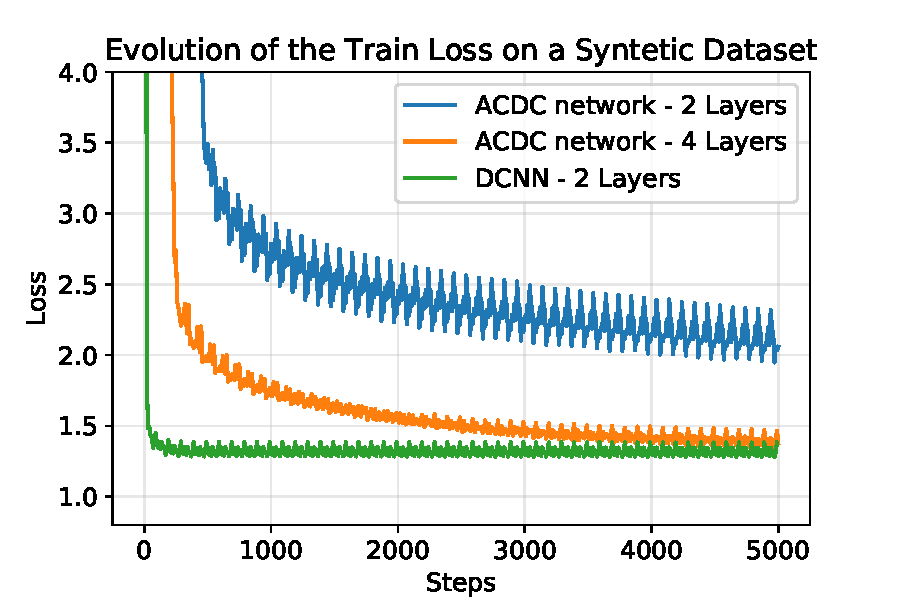
\includegraphics[width=\textwidth]{figures/chapter3/acdc_regression.pdf}
       \caption{Evolution of the training loss on a regression task with synthetic data.}
       \label{figure:acdc_regression}
   \end{subfigure}
   \hfill
   \begin{subfigure}[b]{0.49\textwidth}
       \centering
       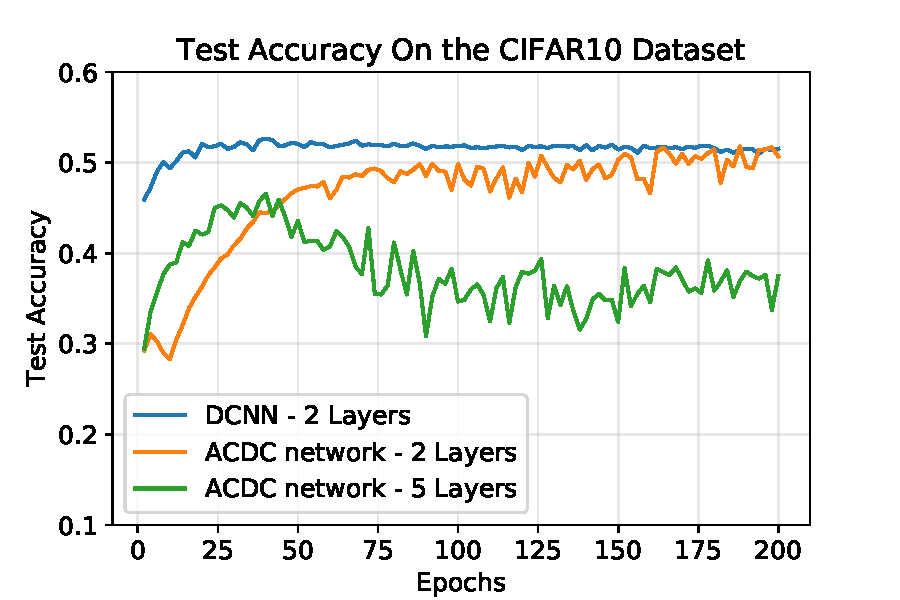
\includegraphics[width=\textwidth]{figures/chapter3/acdc_cifar10.pdf}
       \caption{Test accuracy on the CIFAR-10 dataset.~\\ \phantom{.}}
       \label{figure:acdc_cifar10}
   \end{subfigure}
   \caption{Comparison of DCNNs and \ACDC networks on two different tasks.}
\end{figure}


\paragraph{Comparison with \ACDC \citep{moczulski2015acdc}.}

In Section~\ref{section:ch4-related_work}, we have discussed the differences between the \ACDC framework and our approach from a theoretical perspective.
In this section, we conduct experiments to compare the performance of DCNNs with neural networks based on \ACDC layers. 
We first reproduce the experimental setting from \citet{moczulski2015acdc}, and compare both approaches using only linear networks (\ie networks without any ReLU activations).
The synthetic dataset has been created in order to reproduce the experiment on the regression linear problem proposed by~\citet{moczulski2015acdc}.
We draw $\Xmat$ and $\Wmat$ from a uniform distribution between [-1, +1] and $\epsilon$ from a normal distribution with mean 0 and variance $0.01$.
The relationship between $\Xmat$ and $\Ymat$ is define by $\Ymat = \Xmat\Wmat + \epsilon$. 
The results are presented in Figure~\ref{figure:acdc_regression}.
On this simple setting, while both architectures demonstrate good performance, we can observe that DCNNs offer a better convergence rate.
In Figure~\ref{figure:acdc_cifar10}, we compare neural networks with ReLU activations on CIFAR-10. 

We found that networks which are based only on \ACDC layers are difficult to train and offer poor accuracy on CIFAR-10 (we have tried different initialization schemes including the one from the original paper, and the one we introduce in this chapter).
\citet{moczulski2015acdc} manage to train a large VGG network  however these networks are generally highly redundant and the contribution of the structured layer is difficult to quantify. 
We also observe that adding a single dense layer improves the convergence rate of \ACDC in the linear case, which explains the good results of \citet{moczulski2015acdc}.
However, it is difficult to characterize the true contribution of the \ACDC layers when the network has a large number of expressive layers.

In contrast, deep DCNNs can be trained and offer good performance without additional dense layers (these results are in line with our experiments on the \yt dataset).
We can conclude that DCNNs are able to model complex relations at a low cost. 

\begin{figure}
   \centering
   \begin{tikzpicture}[scale=0.5]
\begin{axis}[
    legend cell align={left},
    xlabel={\large \#weights (x1000) },
    ylabel={Test Accuracy},
    xmin=21, xmax=370,
    ymin=0.2, ymax=0.6,
    legend pos=south east,
    ymajorgrids=true,
    grid style=dashed,
	]
    \addplot[color=red, line width=0.25mm, dashed] table [y=accuracy, x=weights]{figures/chapter3/data/cifar10/type/dense.dat};
    \addplot[mark=triangle, color=blue, line width=0.4mm] table [y=accuracy, x=weights]{figures/chapter3/data/cifar10/type/circulant.dat};
    \addplot[mark=square, color=red, line width=0.4mm] table [y=accuracy, x=weights]{figures/chapter3/data/cifar10/type/diag_toeplitz.dat};
    \addplot[mark=o, color=gray, line width=0.4mm] table [y=accuracy, x=weights]{figures/chapter3/data/cifar10/type/toeplitz.dat};
    \addplot[mark=diamond, color=brown, line width=0.4mm] table [y=accuracy, x=weights]{figures/chapter3/data/cifar10/type/low_rank.dat};
    \legend{
      Dense (9M weights),
      DCNN,
      DTNN,
      Toeplitz network,
      Low Rank network, 
     }
\end{axis}
\end{tikzpicture}

   \caption{Network size vs. Accuracy compared on Dense networks, DCNNs (our approach), DTNNs (our approach), neural networks based on Toeplitz matrices and neural networks based on Low Rank-based matrices. DCNNs outperforms alternatives structured approaches.}
   \label{figure:cifar10_type}
\end{figure}

\begin{figure}
   \centering
   \begin{tikzpicture}[scale=0.5]
\begin{axis}[
    xlabel={\large \#weights (x1000) },
    ylabel={Test Accuracy},
    legend pos=outer north east,
    legend cell align={left},
    ymajorgrids=true,
    grid style=dashed,
    ]
    % \addplot[mark=oplus*,blue] coordinates {(15, 0.6178)}; % Random Conv + Dense
    % \addplot[mark=oplus*,red] coordinates {(90, 0.8438)}; % Conv + Dense
    \addplot[mark=triangle*,blue] coordinates {(140, 0.7017)}; % ldr-sd (rank=1)
    \addplot[mark=triangle*,red] coordinates {(420, 0.7286)}; % ldr-sd (rank=10)
    \addplot[mark=diamond*,blue] coordinates {(110, 0.7111)}; % toeplitz-like (rank=1)
    \addplot[mark=diamond*,red] coordinates {(388, 0.7205)}; % toeplitz-like (rank=10)
    \addplot[mark=square*,green] coordinates {(124, 0.757)}; % Scattering + 1 DC
    \addplot[mark=square*,blue] coordinates {(217, 0.7856)}; % Scattering + 3 DC
    \addplot[mark=square*,red] coordinates {(66, 0.7535)}; % Scattering Avg pooling + 3 DC
    \addplot[mark=square*,brown] coordinates {(191, 0.764)}; % Scattering by channel + 4 DC
    % \addplot[mark=square*,green] coordinates {(131, 0.704)}; % Conv 32 + Max Pooling + 5 DC
    \legend{
        % Random Conv + Dense,
        % Conv + Dense,
        Scattering + LDR-SD (r=1),
        Scattering + LDR-SD (r=10),
        Scattering + Toeplitz-like (r=1),
        Scattering + Toeplitz-like (r=10),
        Scattering + 1 DC,
        Scattering + 3 DC,
        Scattering Avg pooling + 3 DC,
        Scattering by channel + 4 DC,
        % Conv + Max Pooling + DC,
    }
\end{axis}
\end{tikzpicture}

		
   \caption{Accuracy of different structured architecture given the number of trainable parameters.}
   \label{figure:cifar10_with_channels_xp}
\end{figure}


\paragraph{Comparison with Dense networks, Toeplitz networks and Low Rank networks.}
We now compare DCNNs with other state-of-the-art structured networks by measuring the accuracy on a flattened version of the CIFAR-10 dataset.
Our baseline is a dense feed-forward network with a fixed number of weights (9 million weights).
We compare with DCNNs and with DTNNs (see below), Toeplitz networks, and Low-Rank networks~\cite{8099498}.
We first consider Toeplitz networks which are stacked Toeplitz matrices interleaved with ReLU activations since Toeplitz matrices are closely related to circulant matrices.
However, Toeplitz networks have a different structure than DCNNs (they do not include diagonal matrices), therefore, we also experiment using DTNNs, a variant of DCNNs where all the circulant matrices have been replaced by Toeplitz matrices.
Finally we conduct experiments using networks based on low-rank matrices as they are also closely related to our work.
For each approach, we report the accuracy of several networks with a varying depth ranging from 1 to 40 (DCNNs, Toeplitz networks) and from 1 to 30 (from DTNNs).
For low-rank networks, we used a fixed depth network and increased the rank of each matrix from 7 to 40.
We also tried to increase the depth of low rank matrices, but we found that deep low-rank networks are difficult to train so we do not report the results here.
We compare all the networks based on the number of weights from 21K (0.2\% of the dense network) to 370K weights (4\% of the dense network) and we report the results in Figure~\ref{figure:cifar10_type}. 
First we can see that the size of the networks correlates positively with their accuracy which demonstrate successful training in all cases.
We can also see that the DCNNs achieves the maximum accuracy of 56\% with 20 layers ($\sim$ 200K weights) which is as good as the dense networks with only 2\% of the number of weights.
Other approaches also offer good trade-off but they are not able to reach the accuracy of a dense network.


\begin{table}[htb]
  \centering
  \begin{tabular}{lcc}
    \toprule
    \textbf{Architectures} & \textbf{\#Params} & \textbf{Acc.}  \\
    \midrule
    \textit{Dense} & \textit{9.4M}	& \textit{0.562} \\
    \textbf{\textit{DCNN $(5\ layers)$}} & \textbf{49K}	& \textbf{0.543} \\
    \textbf{\textit{DCNN $(2\ layers)$}} & \textbf{21K} & \textbf{0.536} \\
    LDR--TD	$(r = 2)$	        & 64K	& 0.511 \\
    LDR--TD	$(r = 3)$	        & 70K	& 0.473 \\
    Toeplitz-like $(r=2)$	    & 46K	& 0.483 \\
    Toeplitz-like $(r =3)$	    & 52K    & 0.496 \\
    \bottomrule
    \end{tabular}
    \caption{LDR networks compared with DCNNs on a flattend version of CIFAR-10. DCNNs outperform all LDR configurations with fewer weights. Remark: the numbers may differ from the original experiments by~\citet{Thomas_NIPS2018_8119} because we use the original dataset instead of a monochrome version.}
    \label{table:xp_ldr}
\end{table}

\begin{table}[htb]
  \centering
  \begin{tabular}{lcc}
    \toprule
    \textbf{Architectures} & \textbf{\#Params} & \textbf{Acc.}  \\
    \midrule
    \textbf{DC $(1\ layers)$} & \textbf{124K} & \textbf{0.757} \\
    \textbf{DC $(3\ layers)$} & \textbf{217K} & \textbf{0.785} \\
    \textbf{Ensemble x5 DC $(3\ layers)$} &  \textbf{1.08M} & \textbf{0.811} \\
    LDR-SD $(r=1)$ & 140K & 0.701 \\
    LDR-SD $(r=10)$ & 420K & 0.728 \\
    Toeplitz-like $(r=1)$ & 110K & 0.711 \\
    Toeplitz-like $(r=10)$ & 388K & 0.720 \\
    \bottomrule
    \end{tabular}
    \caption{Two depths scattering on CIFAR-10 followed by LDR or DC layer. Networks with DC layers outperform all LDR configurations with fewer weights.}
    \label{table:xp_ldr_scattering}
\end{table}


\paragraph{Comparison with LDR networks~\cite{Thomas_NIPS2018_8119}.}
We now compare DCNNs with the LDR framework using the network configuration experimented in the original paper: a single LDR structured layer followed by a dense layer.
In the LDR framework, we can change the size of a network by adjusting the rank of the residual matrix, effectively capturing matrices with a structure that is close to a known structure but not exactly (in the LDR framework, Toeplitz matrices can be encoded with a residual matrix with rank=2, so a matrix that can be encoded with a residual of rank=3 can be seen as Toeplitz-like.).
The results are presented in Table~\ref{table:xp_ldr} and demonstrate that DCNNs outperforms all LDR networks both in terms in size and accuracy.

\paragraph{Exploiting image features.}
Dense layers and DCNNs are not designed to capture task-specific features such as the translation invariance inherently useful in image classification.
We can further improve the accuracy of such general purpose architectures on image classification without dramatically increasing the number of trained parameters by stacking them on top of fixed (ie non-trained) transforms such as the scattering transform \cite{mallat2010recursive}.
In this section we compare the accuracy of various structured networks, enhanced with the scattering transform, on an image classification task, and run comparative experiments on CIFAR-10. 

Our test architecture consists of 2 depth scattering on the RGB images followed by a batch norm and LDR or DC layer.
To vary the number of parameters of Scattering+LDR architecture, we increase the rank of the matrix (stacking several LDR matrices quickly exhausted the memory).
The Figure \ref{figure:cifar10_with_channels_xp} and \ref{table:xp_ldr_scattering} shows the accuracy of these architectures given the number of trainable parameters.

First, we can see that the DCNN architecture very much benefits from the scattering transform and is able to reach a competitive accuracy over 78\%.
We can also see that scattering followed by a DC layer systematically outperforms scattering + LDR or scattering + Toeplitz-like with less parameters. 


%%%%%%%%%%%%%%%%%%%%%%%%%%%%%%%%%%%%%%%%%%%%%%%%%%%%%%%%%%%%%%%%%%%%%%%%%%%%%%%
\subsection{Comparison with other compression based approaches}
\label{subsection:ch4-comparison_with_other_compression_based_approaches}
%%%%%%%%%%%%%%%%%%%%%%%%%%%%%%%%%%%%%%%%%%%%%%%%%%%%%%%%%%%%%%%%%%%%%%%%%%%%%%%


\begin{table}
  \centering
    \caption{Comparison with compression based approaches}
    \begin{tabular}{lcrc}
    \toprule
    \multicolumn{1}{c}{\textbf{Architecture}} & \multicolumn{1}{c}{\textbf{\#Params}} & \textbf{Error (\%)} \\
    \hline \\
    \textit{LeNet \cite{Lecun98gradient-basedlearning}} & \textit{4 257 674} & \textit{0.61} \\
    \multirow{2}[0]{*}{\textbf{DCNN}} & \textbf{25 620} & \textbf{1.74} \\
          & \textbf{31 764} & \textbf{1.60} \\
    \multirow{2}[0]{*}{HashNet \cite{Chen_Hashing_Trick}} & 46 875 & 2.79 \\
          &  78 125 & 1.99 \\
    \multirow{2}[0]{*}{Dark Knowledge \cite{44873}} & 46 875 & 6.32 \\
          &  78 125 & 2.16 \\
    \bottomrule
    \end{tabular}%
  \label{tab:mnist}%
\end{table}%


We provide a comparison with other compression based approaches such as HashNet \cite{Chen_Hashing_Trick}, Dark Knowledge \cite{44873} and Fast Food Transform (FF) \cite{7410530}. 
Table~\ref{tab:mnist} shows the test error of DCNN against other know compression techniques on the MNIST datasets. We can observe that DCNN outperform easily HashNet \cite{Chen_Hashing_Trick} and Dark Knowledge \cite{44873} with fewer number of parameters. The architecture with Fast Food (FF) \cite{7410530} achieves better performance but with convolutional layers and only $1$ Fast Food Layer as the last Softmax layer. 


%%%%%%%%%%%%%%%%%%%%%%%%%%%%%%%%%%%%%%%%%%%%%%%%%%%%%%%%%%%%%%%%%%%%%%%%%%%%%%%
\subsection{Large-scale video classification on the \yt dataset}
\label{subsection:ch4-large_scale_video_classification}
%%%%%%%%%%%%%%%%%%%%%%%%%%%%%%%%%%%%%%%%%%%%%%%%%%%%%%%%%%%%%%%%%%%%%%%%%%%%%%%

To understand the performance of deep DCNNs on large scale applications, we conducted experiments on the \yt video classification with 3.8 training examples introduced by~\citet{abu2016youtube}.
Notice that we favour this experiment over ImageNet applications because modern image classification architectures involve a large number of convolutional layers, and compressing convolutional layers is out of our scope. 
Also, as mentioned earlier, testing the performance of DCNN architectures mixed with a large number of expressive layers makes little sense.
The \yt includes two datasets describing 8 million labeled videos.
Both datasets contain audio and video features for each video.
In the first dataset (\emph{aggregated}) all audio and video features have been aggregated every 300 frames.
The second dataset (\emph{full}) contains the descriptors for all the frames.
To compare the models we use the GAP metric (Global Average Precision) proposed by~\citet{abu2016youtube}.
On the simpler \emph{aggregated} dataset we compared off-the-shelf DCNNs with a dense baseline with 5.7M weights.
On the full dataset, we designed three new compact architectures based on the state-of-the-art architecture introduced by~\citet{abu2016youtube}. 

\paragraph{Experiments on the aggregated dataset with DCNNs:}
We compared DCNNs with a dense baseline with 5.7 millions weights.
The goal of this experiment is to discover a good trade-off between depth and model accuracy.
To compare the models we use the GAP metric (Global Average Precision) following the experimental protocol in~\cite{abu2016youtube}, to compare our experiments. 

Table~\ref{table:youtube_agg_xp} shows the results of our experiments on the {\em aggrgated} \yt dataset in terms of number of weights, compression rate and GAP.
We can see that the compression ratio offered by the circulant architectures is high.
This comes at the cost of a little decrease of GAP measure.
The 32 layers DCNN is 46 times smaller than the original model in terms of number of parameters while having a close performance. 


\begin{table}
  \centering
  \caption{This table shows the GAP score for the \yt dataset with DCNNs. We can see a large increase in the score with deeper networks.}
  \begin{tabular}{lccc}
    \toprule
    \textbf{Architecture} & \textbf{\#Weights} &
    \textbf{GAP@20} \\
    \hline \\
    \textit{original} & \textit{5.7M} & \textit{0.773} \\
    4 DC & 25 410  (\textit{\textbf{0.44}}) & 0.599   \\
    32 DC  & 122 178 \textit{(2.11)} & 0.685   \\
    4 DC + 1 FC & 4.46M \textit{(77)} & \textbf{0.747} \\
  \hline
  \end{tabular}
  \label{table:youtube_agg_xp}
\end{table}

\begin{table}
  \centering
  \caption{This table shows the GAP score for the \yt dataset with different layer represented with our DC decomposition.}
  \begin{tabular}{lccc}
  \toprule
  \textbf{Architecture} & \textbf{\#Weights} & \textbf{GAP@20} \\
  \hline \\
  \textit{original} & \textit{45M} & \textit{0.846} \\
  DBoF with DC   & 36M (\textit{80}) & 0.838 \\
  FC with DC    & 41M (\textit{91}) & \textbf{0.845} \\
  MoE with DC   & 12M (\textit{\textbf{26}}) & 0.805 \\
  \hline
  \end{tabular}
  \label{table:youtube_full_xp}
\end{table}

\paragraph{Experiments with DCNNs Deep Bag-of-Frames Architecture:}
The Deep Bag-of-Frames architecture can be decomposed into three blocks of layers, as illustrated in Figure~\ref{figure:archi_youtube}.
The first block of layers, composed of the Deep Bag-of-Frames embedding (DBoF), is meant to model an embedding of these frames in order to make a simple representation of each video.
A second block of fully connected layers (FC) reduces the dimensionality of the output of the embedding and merges the resulting output with a concatenation operation.
Finally, the classification block uses a combination of Mixtures-of-Experts (MoE)~\cite{716791,abu2016youtube} and Context Gating~\cite{miech2017learnable} to calculate the final class probabilities.
Table~\ref{table:youtube_full_xp} shows the results in terms of number of weights, size of the model (MB) and GAP on the full dataset, replacing the DBoF block reduces the size of the network without impacting the accuracy.
We obtain the best compression ratio by replacing the MoE block with DCNNs (26\%) of the size of the original dataset with a GAP score of 0.805 (95\% of the score obtained with the original architecture).
We conclude that DCNN are both theoretically sound and of practical interest in real, large scale applications.

\begin{figure}[htb]
  \centering
  \tikzset{%
  >={Latex[width=2mm,length=2mm]},
  % Specifications for style of nodes:
            base/.style = {rectangle, draw=black, text centered, font=\sffamily},
             box/.style = {base, rounded corners, text depth=3cm, minimum height=4cm, minimum width=3cm},
     transparent/.style = {rectangle, draw=black},
       circulant/.style = {base, fill=yellow!30},
       embedding/.style = {base, fill=blue!30, minimum width=2.5cm, minimum height=1cm},
           other/.style = {base, fill=white!30,  minimum width=2cm, minimum height=1cm},
              fc/.style = {base, fill=orange!30, minimum width=1.5cm, minimum height=1cm},
          gating/.style = {base, fill=green!30, minimum width=2cm, text width=2cm, minimum height=1cm},
             moe/.style = {base, fill=purple!30, minimum width=1.5cm, minimum height=1cm},
}

\begin{tikzpicture}[every node/.style={fill=white, font=\sffamily}, align=center]

  \draw (0.0, +2.)  node [other, draw=none] {\textbf{Embedding}};
  \draw (+3.7, +2.)  node [other, draw=none] {\textbf{Dim Reduction}};
  \draw (+8.0, +2.)  node [other, draw=none] {\textbf{Classification}};

  \draw (0, +0.8)  node [embedding] {Video};
  \draw (0, -0.8)  node [embedding] {Audio};

  \draw (+2.5, +0.8)  node (fc) [fc] {FC};
  \draw (+2.5, -0.8)  node (fc) [fc] {FC};

  \draw (+4.75, 0)  node (fc) [other] {concat};
  \draw (+7.0, 0)  node (moe) [moe] {MoE};
  \draw (+9.25, 0)  node (gating2) [gating] {Context Gating};
 
  \draw (+1.5, +2) [dashed] -- (+1.5, -1.7);
  \draw (+6, +2) [dashed] -- (+6, -1.7);
  
\end{tikzpicture}

  \caption{This figure shows the state-of-the-art neural network architecture, initially proposed by~\citet{abu2016youtube} and later improved by~\citet{miech2017learnable}, used in our experiment.}
  \label{figure:archi_youtube}
\end{figure}

\paragraph{Architectures \& Hyper-Parameters:} 
For the first set of our experiments (\emph{experiments on CIFAR-10}), we train all networks for 200 epochs, a batch size of 200, Leaky ReLU activation with a different slope.
We minimize the Cross Entropy Loss with Adam optimizer and use a piecewise constant learning rate of $5 \times 10^{-5}$, $2.5\times10^{-5}$, $5\times10^{-6}$ and $1\times10^{-6}$ after respectively 40K, 60K and 80K steps.
For the \yt dataset experiments, we built a neural network based on the SOTA architecture initially proposed by~\citet{abu2016youtube} and later improved by~\citet{miech2017learnable}.
Remark that no convolution layer is involved in this application since the input vectors are embeddings of video frames processed using state-of-the-art convolutional neural networks trained on ImageNet.
We trained our models with the CrossEntropy loss and used Adam optimizer with a 0.0002 learning rate and a 0.8 exponential decay every 4 million examples.
All fully connected layers are composed of 512 units.
DBoF, NetVLAD and NetFV are respectively 8192, 64 and 64 of cluster size for video frames and 4096, 32, 32 for audio frames.
We used 4 mixtures for the MoE Layer.
We used all the available 300 frames for the DBoF embedding.
In order to stabilize and accelerate the training, we used batch normalization before each non linear activation and gradient clipping. 

%%%%%%%%%%%%%%%%%%%%%%%%%%%%%%%%%%%%%%%%%%%%%%%%%%%%%%%%%%%%%%%%%%%%%%%%%%%%%%%
\section{Conclusion}
\label{section:ch4-conclusion}
%%%%%%%%%%%%%%%%%%%%%%%%%%%%%%%%%%%%%%%%%%%%%%%%%%%%%%%%%%%%%%%%%%%%%%%%%%%%%%%

This chapter deals with the training of diagonal circulant neural networks.
To the best of our knowledge, training such networks with a large number of layers had not been done before.
We also endowed this kind of models with theoretical guarantees, hence enriching and refining previous theoretical work from the literature.
More importantly, we showed that DCNNs outperform their competing structured alternatives, including the very recent general approach based on LDR networks.
Our results suggest that stacking diagonal circulant layers with non linearities improves the convergence rate and the final accuracy of the network.
Formally proving these statements constitutes the future directions of this work.
We would like to generalize the good results of DCNNs to convolutional neural networks.
We also believe that circulant matrices deserve a particular attention in deep learning because of their strong ties with convolutions: a circulant matrix operator is equivalent to the convolution operator with circular paddings.
This fact makes any contribution to the area of circulant matrices particularly relevant to the field of deep learning with impacts beyond the problem of designing compact models.
As future work, we would like to generalize our results to deep convolutional neural networks. 



  %%%%%%%%%%%%%%%%%%%%%%%%%%%%%%%%%%%%%%%%%%%%%%%%%%%%%%%%%%%%%%%%%%%%%%%%%%%%%%%
\chapter{Lipschitz Bound of Convolutional Layers}
\label{chapter:lipschitz_bound}
%%%%%%%%%%%%%%%%%%%%%%%%%%%%%%%%%%%%%%%%%%%%%%%%%%%%%%%%%%%%%%%%%%%%%%%%%%%%%%%
\localtableofcontents

% \begin{abstract}
% This paper tackles the problem of Lipschitz regularization of Convolutional Neural Networks. Lipschitz regularity is now established as a key property of modern deep learning with implications in training stability, generalization, robustness against adversarial examples, etc. However, computing the exact value of the Lipschitz constant of a neural network is known to be NP-hard. Recent attempts from the literature introduce upper bounds to approximate this constant that are either efficient but loose or accurate but computationally expensive. In this work, by leveraging the theory of Toeplitz matrices, we introduce a new upper bound for convolutional layers that is both tight and easy to compute. Based on this result we devise an algorithm to train Lipschitz regularized Convolutional Neural Networks.
% \end{abstract}


%%%%%%%%%%%%%%%%%%%%%%%%%%%%%%%%%%%%%%%%%%%%%%%%%%%%%%%%%%%%%%%%%%%%%%%%%%%%%%%
\section{Introduction}
\label{section:ch5-introduction}
%%%%%%%%%%%%%%%%%%%%%%%%%%%%%%%%%%%%%%%%%%%%%%%%%%%%%%%%%%%%%%%%%%%%%%%%%%%%%%%

%%%%%%%%%%%%%%%%%%%%%%%%%%%%%%%%%%%%%%%%%%%%%%%%%%%%%%%%%%%%%%%%%%%%%%%%%%%%%%%
\section{A Primer on Toeplitz and block Toeplitz matrices}
\label{section:primer_toeplitz_matrix}
%%%%%%%%%%%%%%%%%%%%%%%%%%%%%%%%%%%%%%%%%%%%%%%%%%%%%%%%%%%%%%%%%%%%%%%%%%%%%%%

% \subsection{Convolution as Matrix Multiplication}\label{section:conv_matrix_multiplication}
%
% A discrete convolution between a signal $\mathbf{x}$ and a kernel $\mathbf{k}$ can be expressed as a  product between the vectorization of $\mathbf{x}$ and a doubly-block Toeplitz matrix $\textbf{M}$, whose coefficients have been chosen to match the convolution $\mathbf{x} * \mathbf{k}$.
% For a 2-dimensional signal $\mathbf{x} \in \mathbb{R}^{n \times n}$ and a kernel $\mathbf{k} \in \mathbb{R}^{m \times m}$ with $m$ odd, the convolution operation can be written as follows:
% \begin{equation} \label{equation:equation_conv_as_matrix}
%     \reshape(\mathbf{y}) = \reshape(\pad(\mathbf{x}) * \mathbf{k}) = \Mmat \reshape(\mathbf{x})
% \end{equation}
% where $\Mmat$ is a $n^2$-by-$n^2$  doubly-block Toeplitz matrix, \ie a block Toeplitz matrix where the blocks are also Toeplitz (Note that this is not a doubly-block circulant matrix because of the padding.), $\mathbf{y}$ is the output of size $q \times q$ with $q = n - m + 2p + 1$, (see \eg \cite{dumoulin2016guide}).
% The $\reshape: \mathbb{R}^{n \times n} \rightarrow \mathbb{R}^{n^2}$ operator is defined as follows: $\reshape(\mathbf{x})_q = \mathbf{x}_{\lfloor q/n \rfloor,\ q\mod n}$.
% The $\pad: \mathbb{R}^{n \times n} \rightarrow \mathbb{R}^{(n+2p) \times (n+2p)}$ operator is a zero-padding operation which takes a signal $\mathbf{x}$ of shape $\mathbb{R}^{n \times n}$ and adds $0$ on the edges so as to obtain a new signal $\mathbf{y}$ of shape $\mathbb{R}^{(n+2p) \times (n+2p)}$.
% In order to have the same shape between the convoluted signal and the signal, we set $ p = \lfloor m/2 \rfloor$ \footnote{We take a square signal and an odd size square kernel to simplify the notation but the same applies for any input and kernel size.
% Also, we take a specific padding in order to have the same size between the input and output signal.
% But everything in the paper can be generalized to any paddings.}.
%
% We now present an example of the convolution operation with doubly-block Toeplitz matrix.
% Let us define a kernel $\mathbf{k} \in \mathbb{R}^{3\times3}$ as follows:
% \begin{equation}
%     \mathbf{k} = \begin{pmatrix}
%         k_{0} & k_{1} & k_{2} \\
%         k_{3} & k_{4} & k_{5} \\
%         k_{6} & k_{7} & k_{8} 
%     \end{pmatrix}
% \end{equation}
% If we set the padding to 1, then, the matrix $\Mmat$ is a tridiagonal doubly-block Toeplitz matrix of size $n \times n$ and has the following form:
% \begin{equation}
%     \Mmat = \begin{pmatrix}
%     \Tmat_0 & \Tmat_{1} &  &  & 0  \\
%     \Tmat_{2} & \Tmat_0 & \Tmat_{1} &  &  \\
%      & \Tmat_{2} & \scalebox{.70}{$\ddots$} & \scalebox{.70}{$\ddots$} &   \\
%      &  & \scalebox{.70}{$\ddots$} & \Tmat_0 & \Tmat_{1}  \\
%     0 &  &  & \Tmat_{2} & \Tmat_0  \\
%     \end{pmatrix}
%     \label{equation:operator_matrix}
% \end{equation}
%
% where $\Tmat_j$ are banded Toeplitz matrices and the values of $\mathbf{k}$ are distributed in the Toeplitz blocks as follow:
% \begin{align}
% \Tmat_0 = \begin{psmallmatrix}
%     k_{4} & k_{3} &  &  &  0 \\
%     k_{5} & k_{4} & k_{3} &  &   \\
%      & k_{5} & \scalebox{.40}{$\ddots$} & \scalebox{.40}{$\ddots$}  \\
%      &  &  \scalebox{.40}{$\ddots$} & k_{4} & k_{3}  \\
%     0 &  &  & k_{5} & k_{4}  \\
%     \end{psmallmatrix} &&
% \Tmat_{1} = \begin{psmallmatrix}
%     k_{7} & k_{6} &  &  &  0 \\
%     k_{8} & k_{7} & k_{6} &  &   \\
%      & k_{8} & \scalebox{.40}{$\ddots$} & \scalebox{.40}{$\ddots$} &    \\
%      &  &  \scalebox{.40}{$\ddots$} & k_{7} & k_{6}  \\
%     0 &  &  & k_{8} & k_{7}  \\
%     \end{psmallmatrix} &&
% \Tmat_{2} = \begin{psmallmatrix}
%     k_{1} & k_{0} &  &  &  0 \\
%     k_{2} & k_{1} & k_{0} &  &   \\
%      & k_{2} & \scalebox{.40}{$\ddots$} & \scalebox{.40}{$\ddots$} &    \\
%      &  &  \scalebox{.40}{$\ddots$} & k_{1} & k_{0}  \\
%     0 &  &  & k_{2} & k_{1}  \\
%     \end{psmallmatrix} 
% \end{align}
%
%
% \paragraph{Remark 1: } Note that the size of the operator matrix $\Mmat$ of a convolution operation depends on the size of the signal. If a signal $\mathbf{x}$ has size $n \times n$, the vectorized signal will be of size $n^2$ and the operator matrix will be of size $n^2 \times n^2$ which can be very large. Indeed, in deep learning practice the size of the images used for training can range from 32 (CIFAR-10) to hundred for high definition images (ImageNet). Therefore, with classical methods, computing the singular values of this operator matrix can be very expensive.
%
% \paragraph{Remark 2: } In the particular case of zero padding convolution operation, the operator matrix is a Toeplitz block with circulant block (i.e. each block of the Toeplitz block is a circulant matrix) which is a particular case of doubly-block Toeplitz matrices. 


\subsection{Generating a Toeplitz matrix and block Toeplitz matrix from a trigonometric polynomial}
An $n\times n$ Toeplitz matrix $\mathbf A$ is fully determined by a two-sided sequence of scalars: $\{a_\seqidx\}_{\seqidx \in \seqsetN}$, whereas an $nm\times nm$ block Toeplitz matrix $\Bmat$ is fully determined by a two-sided sequence of blocks $\{\Bmat_\seqidx\}_{\seqidx \in \seqsetN}$ and where each block $\Bmat_\seqidx$ is an $m \times m$ matrix.  

\begin{equation}
    \Amat \triangleq  \begin{psmallmatrix}
      a_0 & a_{1}   & a_{2} & \cdots & \cdots & a_{n-1}  \\
      a_{-1} & a_0 & a_{1} & \ddots & & \vdots \\
      a_{-2} & a_{-1} & \ddots & \ddots & \ddots & \vdots \\ 
     \vdots & \ddots & \ddots & \ddots & a_{1} & a_{2}\\
     \vdots & & \ddots & a_{-1} & a_{0} & a_{1} \\
    a_{-n+1} & \cdots & \cdots & a_{-2} & a_{-1} & a_0
    \end{psmallmatrix} \quad \quad
    \Bmat \triangleq  \begin{psmallmatrix}
      \Bmat_0 & \Bmat_{1}   & \Bmat_{2} & \cdots & \cdots & \Bmat_{n-1}  \\
      \Bmat_{-1} & \Bmat_0 & \Bmat_{1} & \ddots & & \vdots \\
      \Bmat_{-2} & \Bmat_{-1} & \ddots & \ddots & \ddots & \vdots \\ 
     \vdots & \ddots & \ddots & \ddots & \Bmat_{1} & \Bmat_{2}\\
     \vdots & & \ddots & \Bmat_{-1} & \Bmat_{0} & \Bmat_{1} \\
    \Bmat_{-n+1} & \cdots & \cdots & \Bmat_{-2} & \Bmat_{-1} & \Bmat_0
    \end{psmallmatrix}
\end{equation}

The trigonometric polynomial that \emph{generates} the Toeplitz matrix $\Amat$ can be defined as follows:
\begin{equation}
    f_{\Amat}(\omega) \triangleq \sum_{h \in N} a_h e^{\ci h \omega}
\end{equation}
The function $f_{\Amat}$ is said to be the \emph{generating function} of $\Amat$. To recover the Toeplitz matrix from its generating function, we have the following operator presented in Section~\ref{subsection:generating_function} of the main paper:
\begin{equation} \label{equation:toeplitz_operator}
    \leftmat \Tmat(f) \rightmat_{i, j} \triangleq  \frac{1}{2\pi} \int_0^{2\pi} e^{-\ci (i - j)\omega} f(\omega) \,d\omega .
\end{equation}
We can now show that $\Tmat(f_{\Amat}) = \Amat$: 
\begingroup
\allowdisplaybreaks
\begin{align}
    \leftmat \Tmat(f_\Amat) \rightmat_{i, j} &= \frac{1}{2\pi} \int_0^{2\pi} e^{-\ci (i-j)\omega} f_{\Amat}(\omega) \,d\omega  \\
    &= \frac{1}{2\pi} \int_0^{2\pi} e^{-\ci (i-j) \omega} \sum_{h \in N} a_h e^{\ci h \omega} \,d\omega  \\
    &= \frac{1}{2\pi} \int_0^{2\pi} \sum_{h \in N} a_h e^{\ci (j - i + h) \omega} \,d\omega  \\
    &= \sum_{h \in N} a_h \frac{1}{2\pi} \int_0^{2\pi} e^{\ci (j - i + h) \omega} \,d\omega 
    = a_{j-i} .
\end{align}
\endgroup
Because:
\begin{equation}
    \frac{1}{2\pi} \int_0^{2\pi} e^{\ci k \omega} \,d\omega = \left\{
                \begin{array}{ll}
                  1, & \text{if}\ k = 0, \\
                  0, & \text{if}\ k\ \text{is a non-zero integer number.}
                \end{array}
                \right.
\end{equation}

The same reasoning can be applied to block Toeplitz matrices. Instead of being complex-valued, the trigonometric polynomial that {\em generates} the block Toeplitz $\Bmat$ is matrix-valued and can be defined as follows:
\begin{equation}
    f_{\Bmat}(\omega) \triangleq \sum_{h \in N} \Bmat_h e^{\ci h \omega}
\end{equation}

The function $f_{\Bmat}$ is said to be the \emph{generating function} of $\Bmat$. To recover the block Toeplitz matrix from its generating function, we use the Toeplitz operator defined in Equation~\ref{equation:toeplitz_operator}. We can show that $\Tmat(f_\Bmat) = \Bmat$:

\begingroup
\allowdisplaybreaks
\begin{align}
    \leftmat \Tmat(f_\Bmat) \rightmat_{i, j} &= \frac{1}{2\pi} \int_0^{2\pi} e^{-\ci (i-j)\omega} f_{\Bmat}(\omega) \,d\omega  \\
    &= \frac{1}{2\pi} \int_0^{2\pi} e^{-\ci (i-j) \omega} \sum_{h \in N} \Bmat_h e^{\ci h \omega} \,d\omega  \\
    &= \frac{1}{2\pi} \int_0^{2\pi} \sum_{h \in N} \Bmat_h e^{\ci (j - i + h) \omega} \,d\omega  \\
    &= \sum_{h \in N} \Bmat_h \frac{1}{2\pi} \int_0^{2\pi} e^{\ci (j - i + h) \omega} \,d\omega 
    = \Bmat_{j-i} .
\end{align}
\endgroup




In order to devise a bound on the Lipschitz constant of a convolution layer as used by the Deep Learning community, we study the properties of doubly-block Toeplitz matrices.
In this section, we first introduce the necessary background on Toeplitz and block Toeplitz matrices, and introduce a new result on doubly-block Toeplitz matrices.

Toeplitz matrices and block Toeplitz matrices are well-known types of structured matrices.
A Toeplitz matrix  (respectively a block Toeplitz matrix) is a matrix in which each scalar (respectively block) is repeated identically along diagonals.

An $n \times n$ Toeplitz matrix $\Amat$ is fully determined by a two-sided sequence of scalars: $\{a_\seqidx\}_{\seqidx \in \seqsetN}$, whereas an $nm\times nm$ block Toeplitz matrix $\Bmat$ is fully determined by a two-sided sequence of blocks $\{\Bmat_\seqidx\}_{\seqidx \in \seqsetN}$, where $\seqsetN = \{-n+1,\dots, n-1 \}$ and where each block $\Bmat_\seqidx$ is an $m \times m$ matrix.  

\begin{equation*}
  \Amat = \leftmatrix
    a_0 & a_{1} & \cdots & a_{n-1} \\ \vspace{0.1cm}
    a_{-1} & a_0 & \ddots & \vdots \\ \vspace{0.3cm}
   \vdots & \ddots & a_{0} & a_{1} \\ 
  a_{-n+1} & \cdots  & a_{-1}    & a_0 
  \rightmatrix \quad \quad \quad \quad 
    \Bmat = \leftmatrix
    \Bmat_0 & \Bmat_{1} & \cdots & \Bmat_{n-1} \\ \vspace{0.1cm}
    \Bmat_{-1} & \Bmat_0 & \ddots & \vdots \\ \vspace{0.3cm}
   \vdots & \ddots & \Bmat_0 & \Bmat_{1} \\ 
  \Bmat_{-n+1} & \cdots  & \Bmat_{-1}  & \Bmat_0 
  \rightmatrix.
\end{equation*}

Finally, a doubly-block Toeplitz matrix is a block Toeplitz matrix in which each block is itself a Toeplitz matrix.
In the remainder, we will use the standard notation $\leftmat\ \cdot\ \rightmat_{i,j \in \{0,\ldots,n-1\}}$ to construct (block) matrices.
For example, $\Amat = \leftmat a_{j-i} \rightmat_{i,j \in \{0,\ldots,n-1\}}$ and $\Bmat = \leftmat \Bmat_{j-i} \rightmat_{i,j \in \{0,\ldots,n-1\}}$.

\subsection{Bound on the singular value of Toeplitz and block Toeplitz matrices}
\label{subsection:generating_function}

A standard tool for manipulating (block) Toeplitz matrices is the use of Fourier analysis.
Let $\{a_\seqidx\}_{\seqidx \in \seqsetN}$ be the sequence of coefficients of the Toeplitz matrix $\Amat \in \mathbb{R}^{n\times n}$ and let $\{\Bmat_\seqidx\}_{\seqidx \in \seqsetN}$ be the sequence of $m\times m$ blocks of the block Toeplitz matrix $\Bmat$.
The complex-valued function $f(\omega) = \sum_{\seqidx \in \seqsetN} a_\seqidx e^{\ci \seqidx \omega}$ and the matrix-valued function $F(\omega) = \sum_{\seqidx \in \seqsetN} \Bmat_\seqidx e^{\ci \seqidx \omega}$ are the \emph{inverse Fourier transforms} of the sequences $\{a_\seqidx\}_{\seqidx \in \seqsetN}$ and $\{\Bmat_\seqidx\}_{\seqidx \in \seqsetN}$, with $\omega \in \mathbb{R}$.
From these two functions, one can recover these two sequences using the standard Fourier transform:

\begin{equation}
    a_\seqidx = \frac{1}{2\pi} \int_0^{2\pi} e^{-\ci \seqidx \omega} f(\omega) d\omega \quad \quad \Bmat_\seqidx = \frac{1}{2\pi} \int_0^{2\pi} e^{-\ci \seqidx \omega} F(\omega) d\omega .
\end{equation}

From there, similarly to the work done by~\citet{gray2006toeplitz,gutierrez2012block}, we can define an operator $\Tmat$ mapping integrable functions to matrices:

\begin{equation}
  \Tmat(g)  \triangleq\leftmat\frac{1}{2\pi}\int_{0}^{2\pi}e^{-\ci(i-j)\omega}g(\omega)\,d\omega\rightmat_{i,j\in\{0,\ldots,n-1\}} . \label{equation:expression_toeplitz_matrix}
\end{equation}

Note that if $f$ is the inverse Fourier transform of $\{a_\seqidx\}_{\seqidx \in \seqsetN}$, then $\Tmat(f)$ is equal to $\Amat$.
Also, if $F$ is the inverse Fourier transform of $\{\Bmat_\seqidx\}_{\seqidx \in \seqsetN}$ as defined above, then the integral in Equation~\ref{equation:expression_toeplitz_matrix} is matrix-valued, and thus $\Tmat(F) \in \mathbb{R}^{mn \times mn}$ is the block matrix $\Bmat$.

Now, we can state two known theorems which upper bound the maximal singular value of Toeplitz and block Toeplitz matrices with respect to their generating functions.
In the rest of the paper, we refer to $\sigma_1(\ \cdot\ )$ as the maximal singular value. 

\begin{theorem}[Bound on the singular values of Toeplitz matrices] \label{theorem:teoplitz_sup_singular}
Let $f: \mathbb{R} \rightarrow \mathbb{C}$, be continuous and $2\pi$-periodic. Let $\Tmat(f) \in \mathbb{R}^{n \times n}$ be a Toeplitz matrix generated by the function $f$, then:
\begin{align}
  \sigma_1 \left( \Tmat(f) \right) \leq \sup_{\omega \in [0, 2\pi]} |f(\omega)|.
\end{align}
\end{theorem}

Theorem~\ref{theorem:teoplitz_sup_singular} is a direct application of  Lemma 4.1 by~\citet{gray2006toeplitz} for real Toeplitz matrices. 
\begin{theorem}[Bound on the singular values of Block Toeplitz matrices ~\citet{gutierrez2012block}] \label{theorem:block_teoplitz_sup_singular}
Let $F: \mathbb{R} \rightarrow \mathbb{C}^{m \times m}$ be a matrix-valued function which is continuous and $2 \pi$-periodic.
Let $\Tmat(F) \in \mathbb{R}^{mn \times mn}$ be a block Toeplitz matrix generated by the function $F$, then:
\begin{align}
  \sigma_1 \left( \Tmat(F) \right) \leq \sup_{\omega \in [0, 2\pi]} \sigma_1 \left( F\left( \omega \right) \right) .
\end{align}
\end{theorem}

\subsection{Bound on the singular value of Doubly-Block Toeplitz matrices}
\label{section:bound_singular_value_doubly_block_toeplitz}

We extend the reasoning from Toeplitz and block Toeplitz matrices to doubly-block Toeplitz matrices (\ie block Toeplitz matrices where each block is also a Toeplitz matrix).
A doubly-block Toeplitz matrix can be generated by a function $f: \mathbb{R}^2 \rightarrow \mathbb{C}$ using the 2-dimensional inverse Fourier transform.
For this purpose, we define an operator $\Dmat$ which maps a function $f: \mathbb{R}^2 \rightarrow \mathbb{C}$ to a doubly-block Toeplitz matrix of size $nm \times nm$.
For the sake of clarity, the dependence of $\Dmat(f)$  on $m$ and $n$ is omitted.
Let $\Dmat(f) =\leftmat\Dmat_{i,j}(f)\rightmat_{i,j\in\{0,\ldots ,n-1\}}$ where $\Dmat_{i,j}$ is defined as:
\begin{equation} \label{equation:doubly_block_toeplitz_operator}
  \Dmat_{i,j}(f) = \leftmat \frac{1}{4\pi^{2}} \int_{[0,2\pi]^{2}} e^{- \ci \left((i-j)\omega_{1}+(k-l)\omega_{2}\right)}f(\omega_{1},\omega_{2})\,d(\omega_{1},\omega_{2}) \rightmat_{k,l\in\{0,\ldots,m-1\}} .
\end{equation}

We are now able to combine Theorem~\ref{theorem:teoplitz_sup_singular} and Theorem~\ref{theorem:block_teoplitz_sup_singular} to bound the maximal singular value of doubly-block Toeplitz matrices with respect to their generating functions. 

Note that in the following, we only consider generating functions as trigonometric polynomials with real coefficients therefore the matrices generated by $\Dmat(f)$ are real. We can now combine Theorems~\ref{theorem:teoplitz_sup_singular} and~\ref{theorem:block_teoplitz_sup_singular} to bound the maximal singular value of a doubly-block Toeplitz Matrix. 

\begin{theorem}[Bound on the maximal singular value of a Doubly-Block Toeplitz Matrix] \label{theorem:doubly_block_teoplitz_sup_singular}
Let $\Dmat(f) \in \mathbb{R}^{nm \times nm}$ be a doubly-block Toeplitz matrix generated by the function $f$, then:
\begin{align}
  \sigma_{1} \left( \Dmat(f) \right) &\leq \sup_{\omega_1, \omega_2 \in [0, 2\pi]^2}|f(\omega_1,\omega_2)|
\end{align}
where the function $f: \mathbb{R}^2 \rightarrow \mathbb{C}$, is a multivariate trigonometric polynomial of the form:
\begin{equation}\label{equation:muli_variate_poly_on_M}
    f(\omega_1, \omega_2) \triangleq \sum_{h_1 \in \seqsetN} \sum_{h_2 \in \seqsetM} d_{h_1, h_2} e^{\ci (h_1 \omega_1 + h_2 \omega_2)},
\end{equation}
where $d_{h_{1},h_{2}}$ is the ${h_2}^\textrm{th}$ scalar of the ${h_1}^\textrm{th}$ block of the doubly-Toeplitz matrix $\Dmat(f)$, and where $\seqsetM = \{-m+1,\dots, m-1 \}$.
\end{theorem}


\begin{proof}[\proofrefth{theorem:doubly_block_teoplitz_sup_singular}]
A doubly-block Toeplitz matrix is by definition a block matrix where each block is a Toeplitz matrix. We can then express a doubly-block Toeplitz matrix with the operator $\Tmat(F)$ where the matrix-valued generating function $F$ has Toeplitz coefficient. Let us define a matrix-valued trigonometric polynomial $F:\mathbb{R}\rightarrow\mathbb{C}^{n \times n}$ of the form:
\begin{equation}
    F(\omega_1) = \sum_{h_1 \in N} \Amat_{h_1}e^{\ci h_1\omega_1}
\end{equation}
where $\Amat_{h_1}$ are Toeplitz matrices of size $m \times m$ determined by the sequence $\{d_{h_1, -m+1}, \dots, d_{h_1, m-1} \}$. 
From Theorem~\ref{theorem:block_teoplitz_sup_singular} we have:
\begin{equation}
\sigma_1\left(\Tmat(F) \right) \leq \sup_{\omega_1 \in [0,2\pi] } \sigma_{1}\left( F(\omega_1) \right) \label{equation:th_bound_block_toeplitz}
\end{equation}

Because Toeplitz matrices are closed under addition and scalar product, $F(\omega_1)$ is also a Toeplitz matrix of size $m \times m$. 
We can thus define a function $f:\mathbb{R}^{2} \rightarrow \mathbb{C}$ such that $f(\omega_1,\ \cdot\ )$ is the generating function of $F(\omega_1)$. From Theorem~\ref{theorem:teoplitz_sup_singular}, we can write:
\begin{align}
    \sigma_{1}\left( F(\omega_1) \right) &\leq \sup_{\omega_2 \in [0,2\pi]} \left| f(\omega_1, \omega_2) \right| \\
    \Leftrightarrow \sup_{\omega_1 \in [0,2\pi]} \sigma_{1}\left( F(\omega_1) \right) &\leq  \sup_{\omega_1, \omega_2 \in [0,2\pi]^2} \left| f(\omega_1, \omega_2) \right| \\
    \Leftrightarrow \sigma_1\left(\Tmat(F) \right) &\leq \sup_{\omega_1, \omega_2 \in [0,2\pi]^2} \left| f(\omega_1, \omega_2) \right|
\end{align}
where the function $f$ is of the form:
\begin{equation}
f(\omega_1,\omega_2) = \sum_{h_1 \in N} \sum_{h_2 \in M} d_{h_1, h_2} e^{\ci \left( h_1\omega_1 + h_2 \omega_2\right)}
\end{equation}
Because the function $f(\omega_1,\ \cdot\ )$ is the generating function of $F(\omega_1)$ is it easy to show that the function $f$ is the generating function of $\Tmat(F)$. Therefore, $\Tmat(F) = \Dmat(f)$ which concludes the proof. 
\end{proof}


%%%%%%%%%%%%%%%%%%%%%%%%%%%%%%%%%%%%%%%%%%%%%%%%%%%%%%%%%%%%%%%%%%%%%%%%%%%%%%%
\section{Bound on the Singular Values of Convolutional Layers}
\label{section:bound_lipschitz_cst_conv}
%%%%%%%%%%%%%%%%%%%%%%%%%%%%%%%%%%%%%%%%%%%%%%%%%%%%%%%%%%%%%%%%%%%%%%%%%%%%%%%

From now on, without loss of generality, we will assume that $n=m$ to simplify notations.
It is well known that a discrete convolution operation with a 2d kernel applied on a 2d signal is equivalent to a matrix multiplication with a doubly-block Toeplitz matrix~\cite{jain1989fundamentals}.
However, in practice, the signal is most of the time 3-dimensional (RGB images for instance).
We call the channels of a signal \emph{channels in} denoted $cin$.
The input signal is then of size $cin \times n \times n$.
Furthermore, we perform multiple convolutions of the same signal which corresponds to the number of channels the output will have after the operation.
We call the channels of the output \emph{channels out} denoted $cout$.
Therefore, the kernel, which must take into account \emph{channels in} and \emph{channels out}, is defined as a 4-dimensional tensor of size: $\cout \times \cin \times s \times s$. 

The operation performed by a 4-dimensional kernel on a 3d signal can be expressed by the concatenation (horizontally and vertically) of doubly-block Toeplitz matrices.
Hereafter, we bound the singular value of multiple vertically stacked doubly-block Toeplitz matrices which corresponds to the operation performed by a 3d kernel on a 3d signal.

\begin{theorem}[Bound on the maximal singular value of stacked Doubly-block Toeplitz matrices] \label{theorem:bound_sv_stacked_dbt} 
Consider doubly-block Toeplitz matrices $\Dmat(f_1), \dots, \Dmat(f_{\cin})$ where $f_i: \Rbb^2 \rightarrow \Cbb$ is a generating function.
Construct a matrix $\Mmat$ with $\cin\times n^2$ rows and $n^2$ columns, as follows:
\begin{equation}
  \Mmat \triangleq \leftmat \Dmat^\top(f_1), \dots, \Dmat^\top(f_{\cin}) \rightmat^\top .
\end{equation}
Then, with $f_i$ a multivariate polynomial of the same form as Equation~\ref{equation:muli_variate_poly_on_M}, we have:
\begin{align} \label{equation:bound_asymptotic_equiv}
  \sigma_1 \left( \Mmat \right) &\leq \sup_{\omega_1, \omega_2 \in \left[0, 2\pi\right]^2} \sqrt{ \sum_{i=1}^{\cin} \left|f_i\right (\omega_1, \omega_2)|^2} .
\end{align}
\end{theorem}

In order to prove Theorem~\ref{theorem:bound_sv_stacked_dbt}, we will need the following lemmas:

\begin{lemma}[\citet{zhang2011matrix}] \label{theorem:diff_positive_semidefinite_matrices}
Let $\Amat$ and $\Bmat$ be Hermitian positive semi-definite matrices. If $\Amat - \Bmat$ is positive semi-definite, then:
\begin{equation*}
    \lambda_1 \left( \Bmat \right) \leq \lambda_1 \left( \Amat \right)
\end{equation*}
\end{lemma}

\begin{lemma}[\citet{serra1994preconditioning}] \label{theorem:block_toeplitz_positive_definite}
If the doubly-block Toeplitz matrix $\Dmat(f)$ is generated by a non-negative function $f$ not identically zero, then the matrix $\Dmat(f)$ is positive definite. 
\end{lemma}

\begin{lemma}[\citet{serra1994preconditioning}] \label{theorem:block_toeplitz_hermitian}
If the doubly-block Toeplitz matrix $\Dmat(f)$ is generated by a function $f: \mathbb{R}^2 \rightarrow \mathbb{R}$, then the matrix $\Dmat(f)$ is Hermitian. 
\end{lemma}

\begin{lemma}[\citet{gutierrez2012block}] \label{theorem:properties_block_toeplitz}
Let $f:\mathbb{R}^2 \rightarrow \mathbb{C}$ and $g:\mathbb{R}^2 \rightarrow \mathbb{C}$ be two continuous and $2\pi$-periodic functions. Let $\Dmat(f)$ and $\Dmat(g)$ be doubly-block Toeplitz matrices generated by the function $f$ and $g$ respectively. Then:
\begin{itemize}
    \item $\Dmat^\top(f) = \Dmat(f^*)$
    \item $\Dmat(f) + \Dmat(g) = \Dmat(f + g)$
\end{itemize}
\end{lemma}

Before proving Theorem~\ref{theorem:bound_sv_stacked_dbt}, we generalize the famous Widom identity \cite{widom1976asymptotic} that express the relation between Toeplitz and Hankel matrix to doubly-block Toeplitz and Hankel matrices.
We will need to generalize the doubly-block Toeplitz operator presented in Section~\ref{section:bound_singular_value_doubly_block_toeplitz}.
From now on, without loss of generality, we will assume that $n=m$ to simplify notations. 

Let $\Hmat^{\alpha_p} (f) = \leftmat \Hmat^{\alpha_p}_{i,j}(f) \rightmat_{i,j \in \{0 \ldots n-1 \}}$ where $\Hmat^{\alpha_p}_{i,j}$ is defined as:

\begin{equation}
  \Hmat^{\alpha_p}_{i,j}(f) =\leftmat \frac{1}{4\pi^{2}}\int_{[0,2\pi]^{2}} e^{-\ci \alpha_p(i, j, k, l, \omega_1, \omega_2)}  f(\omega_{1},\omega_{2})\,d(\omega_{1},\omega_{2})
  \rightmat_{k,l \in \{0, \ldots, n-1 \}} .
\end{equation}
Note that as with the operator $\Dmat(f)$ we only consider generating functions as trigonometric polynomials with real coefficients therefore the matrices generated by $\Hmat(f)$ are real. 

We will use the following $\alpha$ functions:
\begin{itemize}
    \item[] $\alpha_0(i, j, k, l, \omega_1, \omega_2) = (-j-i-1)\omega_1 + (k-l)\omega_2$
    \item[] $\alpha_1(i, j, k, l, \omega_1, \omega_2) = (i-j)\omega_1 + (-l-k-1)\omega_2$
    \item[] $\alpha_2(i, j, k, l, \omega_1, \omega_2) = (-j-i-1)\omega_1 + (-l-k-1)\omega_2$
    \item[] $\alpha_3(i, j, k, l, \omega_1, \omega_2) = (-j-i+n)\omega_1 + (-l-k-1)\omega_2$
\end{itemize}
As with the doubly-block Toeplitz operator $\Dmat(f)$, the matrices generated by the operator $\Hmat^{\alpha_p}$ are of size $n^2 \times n^2$. 

We now present the generalization of the Widom identity for Doubly-Block Toeplitz matrices below:
\begin{lemma}[Generalization of Widom Identity] \label{theorem:widom_idenity}
Let $f:\mathbb{R}^2 \rightarrow \mathbb{C}$ and $g:\mathbb{R}^2 \rightarrow \mathbb{C}$ be two continuous and $2\pi$-periodic functions. 
We can decompose the Doubly-Block Toeplitz matrix $\Dmat(fg)$ as follows:
\begin{equation}
    \Dmat(fg) = \Dmat(f)\Dmat(g) + \sum_{p=0}^3 \Hmat^{\alpha_p \top}(f^*) \Hmat^{\alpha_p}(g) + \Qmat \left( \sum_{p=0}^3 \Hmat^{\alpha_p \top}(f) \Hmat^{\alpha_p }(g^*) \right) \Qmat.
\end{equation}
where $\Qmat$ is the anti-identity matrix of size $n^2 \times n^2$.
\end{lemma}


Now we can prove Theorem~\ref{theorem:bound_sv_stacked_dbt} which bounds the maximal singular value of vertically stacked doubly-block Toeplitz matrices with their generating functions. 

\begin{proof}[\proofrefth{theorem:bound_sv_stacked_dbt}]
First, let us observe the following:
\begin{equation}
    \sigma_1^2 \left( \Mmat \right) = \lambda_1 \left( \Mmat^{\top} \Mmat \right) = \lambda_1 \left( \sum_{i=1}^{\cin} \Dmat^{\top} \left(f_i \right) \Dmat (f_i) \right).
\end{equation}

And the fact that:
\begin{align}
    \lambda_1 \left( \sum_{i=1}^{\cin} \Dmat \left(|f_i|^2 \right) \right) \quad &\stackrel{\text{by Lemma~\ref{theorem:properties_block_toeplitz}}}{=} \quad \lambda_1 \left( \Dmat \left( \sum_{i=1}^{\cin} |f_i|^2 \right) \right) \\ 
    \quad &\stackrel{\text{by Lemma~\ref{theorem:block_toeplitz_hermitian}}}{=} \quad \sigma_1 \left( \Dmat \left( \sum_{i=1}^{\cin} |f_i|^2 \right) \right) \\
    \quad &\stackrel{\text{by Theorem~\ref{theorem:doubly_block_teoplitz_sup_singular}}}{\leq} \quad \sup_{\omega_1, \omega_2 \in [0, 2\pi]^2} \sum_{i=1}^{\cin} |f_i(\omega_1, \omega_2)|^2.
\end{align}

To prove the Theorem, we simply need to verify the following inequality:

\begin{equation}
    \lambda_1 \left( \sum_{i=1}^{\cin} \Dmat^{\top} \left(f_i \right) \Dmat (f_i) \right) \leq \lambda_1 \left( \Dmat \left( \sum_{i=1}^{\cin} |f_i|^2 \right) \right). \label{equation:eq2}
\end{equation}

From the positive definiteness of the following matrix:

\begin{equation}
    \Dmat \left( \sum_{i=1}^{\cin} |f_i|^2 \right) - \sum_{i=1}^{\ci} \Dmat^{\top} \left(f_i \right) \Dmat (f_i),
\end{equation}

one can observe that the r.h.s is a real symmetric positive definite matrix by Lemma~\ref{theorem:block_toeplitz_positive_definite} and \ref{theorem:block_toeplitz_hermitian}. Furthermore, the l.h.s is a sum of positive semi-definite matrices. Therefore, if the subtraction of the two is positive semi-definite, one could apply Lemma~\ref{theorem:diff_positive_semidefinite_matrices} to prove the inequality
~\ref{equation:eq2}. 


We know from Lemma~\ref{theorem:widom_idenity} that 
\begin{equation}
    \Dmat(fg) - \Dmat(f)\Dmat(g) = \sum_{p=0}^3 \Hmat^{\alpha_p \top}(f^*) \Hmat^{\alpha_p}(g) + \Qmat \left( \sum_{p=0}^3 \Hmat^{\alpha_p \top}(f) \Hmat^{\alpha_p}(g^*) \right) \Qmat.
\end{equation}
By instantiating $f = f^*$, $g = f$ and with the use of Lemma~\ref{theorem:properties_block_toeplitz}, we obtain:
\begin{align}
    \Dmat(f^* f) - \Dmat(f^*)\Dmat(f)
    &= \Dmat(|f|^2) - \Dmat^{\top}(f)\Dmat(f) \\
    &= \sum_{p=0}^3 \Hmat^{\alpha_p \top}(f)\Hmat^{\alpha_p}(f) + \Qmat \left( \sum_{p=0}^3 \Hmat^{\alpha_p \top}(f^*)\Hmat^{\alpha_p} (f^*) \right) \Qmat . \label{equation:widom_identity_block_topelitz}
\end{align}

From Equation~\ref{equation:widom_identity_block_topelitz}, we can see that the matrix $\Dmat(|f|^2) - \Dmat^{\top}(f)\Dmat(f)$
is positive semi-definite because it can be decomposed into a sum of positive semi-definite matrices.
Therefore, because positive semi-definiteness is closed under addition, we have:
\begin{align}
    \sum_{i=1}^{\cin} \leftmat \Dmat \left( |f_i|^2 \right) - \Dmat^{\top} \left(f_i \right) \Dmat (f_i) \rightmat &\geq 0
\end{align}

By re-arranging and with the use Lemma~\ref{theorem:properties_block_toeplitz}, we obtain:
\begin{align}
   \sum_{i=1}^{\cin} \leftmat \Dmat \left( |f_i|^2 \right) \rightmat - \sum_{i=1}^{\cin} \leftmat \Dmat^{\top} \left(f_i \right) \Dmat (f_i) \rightmat &\geq 0 \\
    \Dmat \left( \sum_{i=1}^{\cin} |f_i|^2 \right) - \sum_{i=1}^{\cin} \leftmat \Dmat^{\top} \left(f_i \right) \Dmat (f_i) \rightmat &\geq 0
\end{align}


We can conclude that the inequality~\ref{equation:eq2} is true and therefore by Lemma~\ref{theorem:diff_positive_semidefinite_matrices} we have:
\begin{align}
    \lambda_1 \left( \sum_{i=1}^{\cin} \Dmat^{\top} \left(f_i \right) \Dmat (f_i) \right) &\leq \lambda_1 \left( \Dmat \left( \sum_{i=1}^{\cin} |f_i|^2 \right) \right) \\
    \Leftrightarrow \sigma_1^2 \left( \Mmat \right) &\leq \sup_{\omega_1, \omega_2 \in [0, 2\pi]^2} \sum_{i=1}^{\cin} |f_i(\omega_1, \omega_2)|^2 \\
    \Leftrightarrow \sigma_1 \left( \Mmat \right) &\leq \sup_{\omega_1, \omega_2 \in [0, 2\pi]^2} \sqrt{ \sum_{i=1}^{\cin} |f_i(\omega_1, \omega_2)|^2 }
\end{align}
which concludes the proof. 
\end{proof}


To have a bound on the full convolution operation, we extend Theorem~\ref{theorem:bound_sv_stacked_dbt} to take into account the number of output channels.
The matrix of a full convolution operation is a block matrix where each block is a doubly-block Toeplitz matrices. Below, we present our main result:

\begin{theorem}[Bound on the maximal singular value on the convolution operation] \label{theorem:bound_max_sv_convolution} 
Let us define doubly-block Toeplitz matrices $\Dmat(f_{11}), \dots, \Dmat(f_{\cin\times \cout})$ where $f_{ij}: \mathbb{R}^2 \rightarrow \mathbb{C}$ is a generating function. Construct a matrix $\Mmat$ with $\cin\times n^2$ rows and $\cout\times n^2$ columns such as
Then, with $f_{ij}$ a multivariate polynomial of the same form as Equation~\ref{equation:muli_variate_poly_on_M}, we have:
\begin{equation} \label{equation:lipbound_sv}
 \sigma_1 \left( \Mmat \right) \leq \sqrt{ \sum_{i=1}^{\cout} \sup_{\omega_1, \omega_2 \in [0, 2\pi]^2} \sum_{j = 1}^{\cin} \left|f_{ij}(\omega_1, \omega_2) \right|^2 } .
\end{equation} 
\end{theorem}


First, in order to prove Theorem~\ref{theorem:bound_max_sv_convolution}, we will need the following lemma which bound the singular values of a matrix constructed from the concatenation of multiple matrix. 

\begin{lemma}[Bound on the singular values of concatenation of matrices] \label{theorem:bound_concatenation_matrices}
Let us define matrices $\Amat_1, \dots, \Amat_p$ with $\Amat_i \in \mathbb{R}^{n \times n}$. Let us construct the matrix $\Mmat \in \mathbb{R}^{n \times pn}$ as follows:
\begin{equation}
    \Mmat \triangleq \leftmat \Amat_1, \dots, \Amat_p \rightmat
\end{equation}
where $\leftmat\ \cdot\ \rightmat$ define the concatenation operation. Then, we can bound the singular values of the matrix $\Mmat$ as follows:
\begin{equation}
    \sigma_1(\Mmat) \leq \sqrt{\sum_{i=1}^p \sigma_1(\Amat_i)^2}
\end{equation}
\end{lemma}
\begin{proof}[\proofreflem{theorem:bound_concatenation_matrices}]
\begin{align}
    \sigma_1\left(\Mmat\right)^2 &= \lambda_1\left(\Mmat \Mmat^\top\right) \\
    &= \lambda_1\left( \sum_{i=1}^p\Amat_i \Amat_i^\top  \right) \\
    &\leq \sum_{i=1}^p \lambda_1\left( \Amat_i \Amat_i^\top  \right) \\
    &\leq \sum_{i=1}^p \sigma_1\left( \Amat_i \right)^2 \\
    \Leftrightarrow \sigma_1\left(\Mmat\right) &\leq \sqrt{\sum_{i=1}^p \sigma_1(\Amat_i)^2}
\end{align}
which concludes the proof.
\end{proof}


\begin{proof}[\proofrefth{theorem:bound_max_sv_convolution}]
Let us define the matrix $\Mmat_i$ as follows:
\begin{equation}
    \Mmat_i = \leftmat \Dmat(f_{1, i})^\top, \dots, \Dmat(f_{\cin, i})^\top \rightmat^\top .
\end{equation}
We can express the matrix $\Mmat$ as the concatenation of multiple $\Mmat_i$ matrices:
\begin{equation}
    \Mmat = \leftmat \Mmat_1, \dots, \Mmat_{\cout} \rightmat
\end{equation}
Then, we can bound the singular values of the matrix $\Mmat$ as follows:
\begin{align}
    \sigma_1\left(\Mmat\right) &\stackrel{\text{by Lemma~\ref{theorem:bound_concatenation_matrices}}}{\leq} \sqrt{\sum_{i=1}^{\cout} \sigma_1(\Mmat_i)^2} \\
    \sigma_1\left(\Mmat\right) &\stackrel{\text{by Theorem~\ref{theorem:bound_sv_stacked_dbt}}}{\leq} \sqrt{\sum_{j=1}^{\cout} \sup_{\omega_1, \omega_2 \in [0, 2\pi]^2} \sum_{i=1}^{\cin} |f_{ij}(\omega_1, \omega_2)|^2 }
\end{align}
which concludes the proof. 
\end{proof}



We can easily express the bound in Theorem~\ref{theorem:bound_max_sv_convolution} with the values of a 4-dimensional kernel.
Let us define a kernel $\mathbf{k} \in \mathbb{R}^{\cout \times \cin \times s \times s}$, a padding $p \in \mathbb{N}$ and $d = \lfloor s / 2 \rfloor$ the degree of the trigonometric polynomial, then:
\begin{equation}
  f_{ij}(\omega_1, \omega_2) = \sum_{h_1 = -d}^d \sum_{h_2 = -d}^d k_{i, j, h_1,h_2} e^{\ci (h_1 \omega_1 + h_2 \omega_2)}.
\end{equation}
where $k_{i, j, h_1,h_2} = \leftmat \mathbf{k} \rightmat_{i, j, a, b}$ with $a =  s - p - 1 + i$ and $b =  s - p - 1 + j$.

In the rest of the paper, we will refer to the bound in Theorem~\ref{theorem:bound_max_sv_convolution} applied to a kernel as $\lipbound$ and we denote $\lipbound(\mathbf{k})$ the Lipschitz upper bound of the convolution performed by the kernel $\mathbf{k}$. 


%%%%%%%%%%%%%%%%%%%%%%%%%%%%%%%%%%%%%%%%%%%%%%%%%%%%%%%%%%%%%%%%%%%%%%%%%%%%%%%
\section{Computation and Performance Analysis of LipBound}
\label{section:computation_performance_lipbound}
%%%%%%%%%%%%%%%%%%%%%%%%%%%%%%%%%%%%%%%%%%%%%%%%%%%%%%%%%%%%%%%%%%%%%%%%%%%%%%%

This section aims at analyzing the bound introduced in Theorem~\ref{theorem:bound_max_sv_convolution}.
First, we present an algorithm to efficiently compute the bound, we analyze its tightness by comparing it against the true maximal singular value.
Finally, we compare the efficiency and the accuracy of our bound against the state-of-the-art. 

\subsection{Computing the maximum modulus of a trigonometric polynomial}\label{subsection:computing_max_modulus_trig_polynomial}


\begin{figure*}[htb]
  \centering
  \begin{minipage}{.24\linewidth}
    \centering
    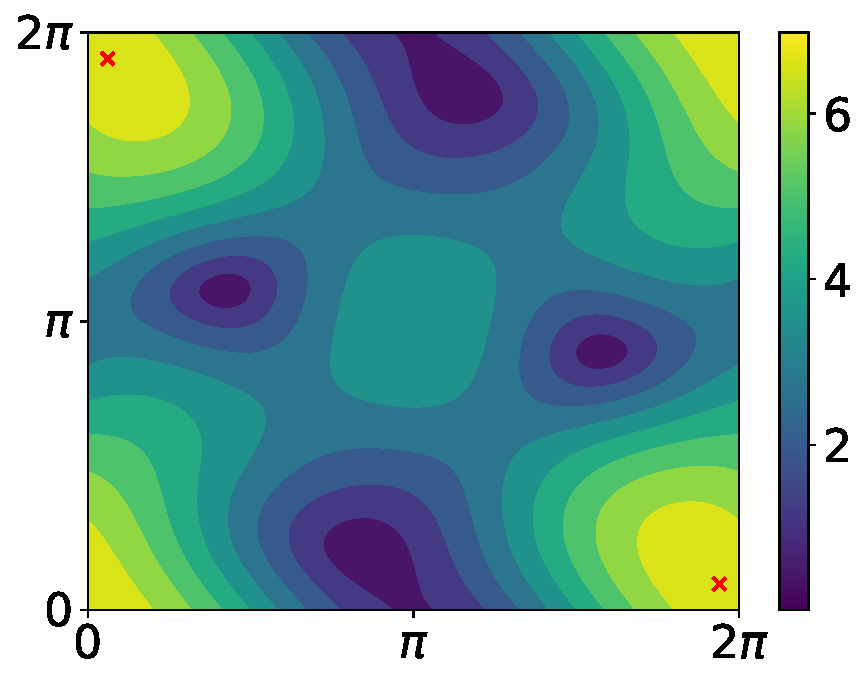
\includegraphics[scale=0.23]{figures/chapter4/contour_poly_200_1_1_3.pdf}\\kernel $1\times3\times3$
  \end{minipage}
  \begin{minipage}{.24\linewidth}
      \centering
      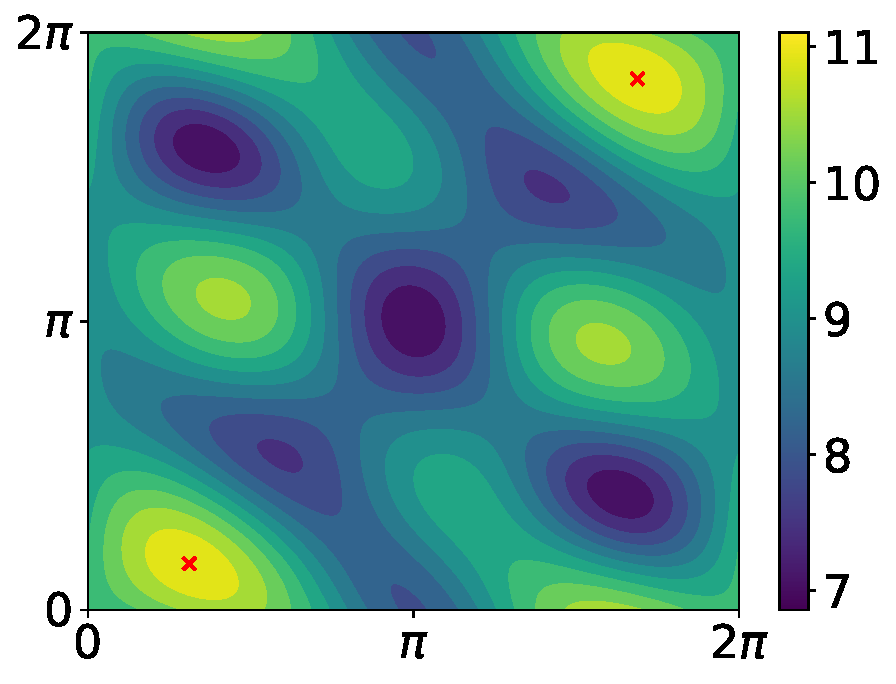
\includegraphics[scale=0.23]{figures/chapter4/contour_poly_200_1_9_3.pdf}\\kernel $9\times3\times3$
  \end{minipage}
  \begin{minipage}{.24\linewidth}
      \centering
      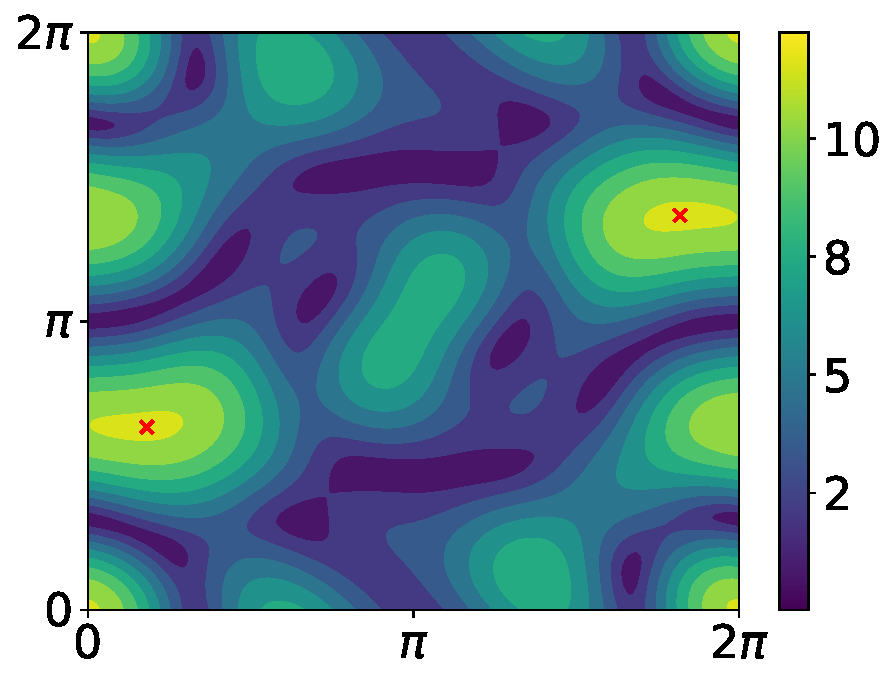
\includegraphics[scale=0.23]{figures/chapter4/contour_poly_200_1_1_5.pdf}\\kernel $1\times5\times5$
  \end{minipage}
  \begin{minipage}{.24\linewidth}
      \centering
      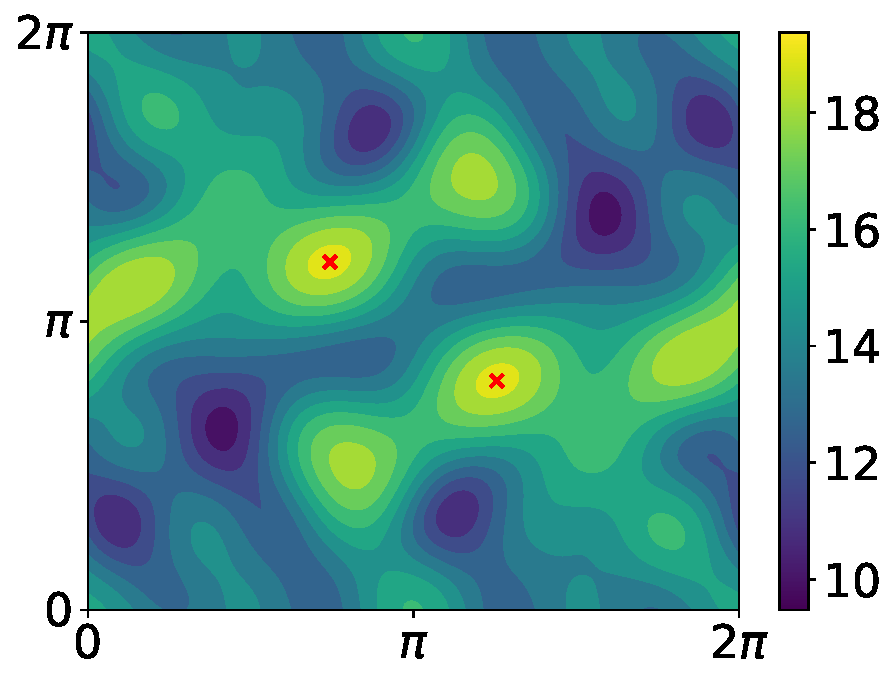
\includegraphics[scale=0.23]{figures/chapter4/contour_poly_200_1_9_5.pdf}\\kernel $9\times5\times5$
  \end{minipage}
  \caption{These figures represent the contour plot of multivariate trigonometric polynomials where the values of the coefficient are the values of a random convolutional kernel. The red dots in the figures represent the maximum modulus of the trigonometric polynomials.}
  \label{figure:contour_plot_trigonometric_polynomials}
\end{figure*}%

\begin{algorithm}
  \caption{PolyGrid Algorithm} \label{algorithm:PolyGrid}
  \begin{algorithmic}[1]
    \Procedure{PolyGrid}{$f, S$}\Comment{polynomial $f$, number of samples $S$}
      \State $\sigma \gets 0$, 
      \State $\omega_1 \gets 0$
      \State $\omega_2 \gets 0$
      \State $\epsilon \gets \frac{2\pi}{S}$
      \For{$i=0$ \textbf{to} $S-1$}
	\For{$j=0$ \textbf{to} $S-1$}
	  \State $\omega_2 \gets \omega_2 + \epsilon$
	  \State $\sigma \gets \max( \sigma, f(\omega_1, \omega_2))$
	\EndFor
      \EndFor
      \State \textbf{return} $\sigma$ \Comment{approximated maximum modulus of $f$}
    \EndProcedure
  \end{algorithmic}
\end{algorithm}

In order to compute $\lipbound$ from Theorem~\ref{theorem:bound_max_sv_convolution}, we have to compute the maximum modulus of several trigonometric polynomials.
However, finding the maximum modulus of a trigonometric polynomial has been known to be NP-Hard~\cite{pfister2018bounding}, and in practice they exhibit low convexity (see Figure~\ref{figure:contour_plot_trigonometric_polynomials}).
We found that for 2-dimensional kernels, a simple grid search algorithm such as PolyGrid (see Algorithm~\ref{algorithm:PolyGrid}), works better than more sophisticated approximation algorithms (\eg ~\citet{green1999calculating,de2009finding}).
This is because the complexity of the computation depends on the degree of the polynomial which is equal to $\lfloor s / 2 \rfloor$ where $s$ is the size of the kernel and is usually small in most practical settings (\eg $s=3$).
Furthermore, the grid search algorithm can be parallelized effectively on CPUs or GPUs and runs within less time than alternatives with lower asymptotic complexity. 

To fix the number of samples $S$ in the grid search, we rely on the work of~\cite{pfister2018bounding}, who has analyzed the quality of the approximation depending on $S$.
Following, this work we first define $\Theta_S$, the set of $S$ equidistant sampling points as follows:
\begin{equation}
  \Theta_S \triangleq \left\{ \omega \mid \omega = k \cdot \frac{2\pi}{S} \mbox{ with }  k = 0,\ldots, S-1 \right\}.
\end{equation}
Then, for a trigonometric polynomial $f: [0, 2\pi]^2 \rightarrow \mathbb{C}$, we have:
\begin{equation}
  \max_{\omega_1, \omega_2 \in [0,2\pi]^2} \left| f(\omega_1, \omega_2) \right| \leq (1 - \alpha)^{-1} \max_{\omega_1', \omega_2' \in \Theta_S^2} \left| f(\omega_1', \omega_2') \right|,
\end{equation}
where $d$ is the degree of the polynomial and $\alpha = 2d / S$.
For a $3\times3$ kernel which gives a trigonometric polynomial of degree 1, we use $S = 10$ which gives $\alpha = 0.2$.
Using this result, we can now compute $\lipbound$ for a convolution operator with $cout$ output channels as per Theorem~\ref{theorem:bound_sv_stacked_dbt}.
 
% The code to for computing $\lipbound$ with NumPy~\cite{numpy} and PyTorch~\cite{paszke2019pytorch} is publicly available.\footnote{\url{https://github.com/MILES-PSL/upper_bound_lipschitz_convolutional_layers}}.


\subsection{Analysis of the tightness of the bound}
\label{section:analysis_tightness_bound}

In this section, we study the tightness of the bound with respect to the dimensions of the doubly-block Toeplitz matrices.
For each $n \in \mathbb{N}$, we define the matrix  $\Mmat^{(n)}$ of size $kn^2 \times n^2$ as follows:
\begin{equation}
  \Mmat^{(n)} \triangleq \textstyle \leftmat \Dmat^{(n)\top}(f_1), \dots, \Dmat^{(n)\top}(f_k) \textstyle \rightmat^\top
\end{equation}
where the matrices $\Dmat^{(n)}(f_i)$ are of size $n^2 \times n^2$. 
To analyze the tightness of the bound, we define the function $\Gamma$, which computes the difference between $\lipbound$ and the maximal singular value of the function $\Mmat^{(n)}$:
\begin{equation} \label{equation:function_convergence}
  \Gamma(n) = \lipbound(\mathbf{k}_{\Mmat^{(n)}}) - \sigma_1(\Mmat^{(n)})
\end{equation}
where $\mathbf{k}_{\Mmat^{(n)}}$ is the  convolution kernel of the convolution defined by the matrix $\Mmat^{(n)}$.

\begin{figure}[ht]
  \centering
  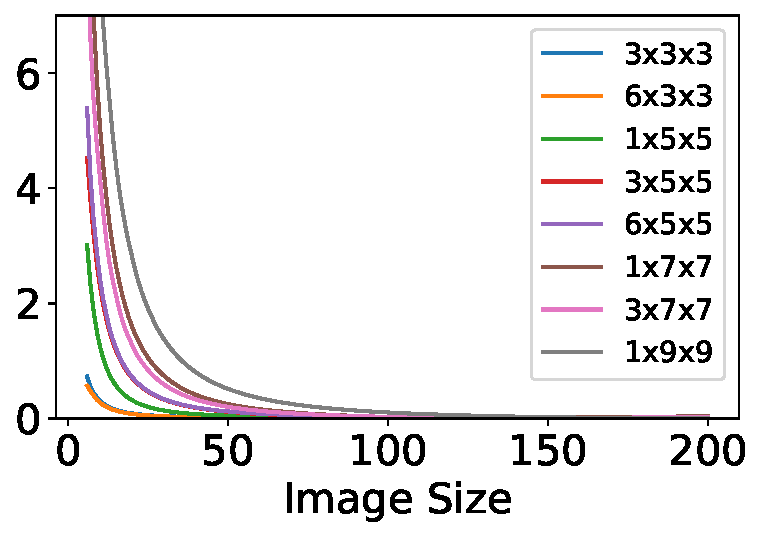
\includegraphics[scale=0.50]{figures/chapter4/convergence_bound.pdf}
  \caption{This graph represents the function $\Gamma(n)$ defined in Section~\ref{section:analysis_tightness_bound} for different kernel size.}
  \label{figure:convergence_bound}
\end{figure}


To compute the exact largest singular value of $\Mmat^{(n)}$ for a specific $n$, we use the Implicitly Restarted Arnoldi Method (IRAM) ~\cite{lehoucq1996deflation} available in SciPy.
The results of this experiment are presented in Figure~\ref{figure:convergence_bound}.
We observe that the difference between the bound and the actual value (approximation gap) quickly decreases as the input size increases.
For an input size of $50$, the approximation gap is as low as $0.012$ using a standard $6\times3\times3$ convolution kernel.
For a larger input size such as ImageNet ($224$), the gap is lower than $4.10^{-4}$.
Therefore $\lipbound$ gives an almost exact value of the maximal singular value of the operator matrix for most realistic settings.

\subsection{Comparison of LipBound with other state-of-the-art approaches} \label{subsection:comparaison_sota}

\begin{table}[ht]
  \centering
  \caption{The following table compares different approaches for computing an approximation of the maximal singular value of a convolutional layer. It shows the ratio between the approximation and the true maximal singular value. The approximation is better for a ratio close to one.}
  {\footnotesize
    \begin{tabular}{lrccrcc}
    \toprule
      &   & \multicolumn{2}{c}{\textbf{1x3x3}} &   & \multicolumn{2}{c}{\textbf{32x3x3}} \\
    \cmidrule{3-4}\cmidrule{6-7}  &   & \textbf{Ratio} & \textbf{Time (ms)} &   & \textbf{Ratio} & \textbf{Time (ms)} \\
    \midrule
    \citeauthor{sedghi2018iclr} &   & $\phantom{.}0.431\pm0.042$ & $1088\pm251$ &   & $\phantom{.}0.666\pm0.123$ & $1729\pm399$ \\
    \citeauthor{singla2019bounding} &   & $\phantom{.}1.293\pm0.126$ & $\phantom{..}1.90\pm0.48$ &   & $\phantom{.}1.441\pm0.188$ & $\phantom{..}1.90\pm0.46$ \\
    \citeauthor{farnia2018generalizable} (10 iter) &   & $\phantom{.}0.973\pm0.006$ & $\phantom{..}4.30\pm0.64$ &   & $\phantom{.}0.972\pm0.004$ & $\phantom{..}4.93\pm0.67$ \\
    \midrule
    \midrule
    \textbf{LipBound (Ours)} &   & $\mathbf{0.992}\pm0.012$ & $\phantom{.}\mathbf{0.49}\pm0.05$ &   & $\mathbf{0.984}\pm0.021$ & $\phantom{.}\mathbf{0.63}\pm0.46$ \\
    \bottomrule
    \end{tabular}%
  }
  \label{table:comparaison}%
\end{table}


In this section we compare our PolyGrid algorithm with the values obtained using alternative approaches.
We consider the 3 alternative techniques by~\citet{sedghi2018iclr,singla2019bounding,farnia2018generalizable} which have been described in Section~\ref{section:ch5-related_work}. 

To compare the different approaches, we extracted 20 kernels from a trained model.
For each kernel we construct the corresponding doubly-block Toeplitz matrix and compute its largest singular value.
Then, we compute the ratio between the approximation obtained with the approach in consideration and the exact singular value obtained by SVD, and average the ratios over the 20 kernels.
Thus good approximations result in approximation ratios that are close to 1.
The results of this experiment are presented in Table~\ref{table:comparaison}.
The comparison has been made on a Tesla V100 GPU. 
The time was computed with the PyTorch CUDA profiler and we warmed up the GPU before starting the timer.

The method introduced by~\citet{sedghi2018iclr} computes an approximation of the singular values of convolutional layers.
We can see in Table~\ref{table:comparaison} that the value is off by an important margin.
This technique is also computationally expensive as it requires computing the SVD of $n^2$ small matrices where $n$ is the size of inputs.
\citet{singla2019bounding} have shown that the singular value of the reshape kernel is a bound on the maximal singular value of the convolution layer.
Their approach is very efficient but the approximation is loose and overestimate the real value.
As said previously, the power method provides a good approximation at the expense of the efficiency.
We use the special Convolutional Power Method from~\citet{farnia2018generalizable} with 10 iterations.
The results show that our proposed technique: PolyGrid algorithm can get the best of both worlds.
It achieves a near perfect accuracy while being very efficient to compute. 

We provide in the supplementary material a benchmark on the efficiency of $\lipbound$ on multiple convolutional architectures. 


%%%%%%%%%%%%%%%%%%%%%%%%%%%%%%%%%%%%%%%%%%%%%%%%%%%%%%%%%%%%%%%%%%%%%%%%%%%%%%%
\section{Application: Lipschitz Regularization for Adversarial Robustness}
\label{section:experiments}
%%%%%%%%%%%%%%%%%%%%%%%%%%%%%%%%%%%%%%%%%%%%%%%%%%%%%%%%%%%%%%%%%%%%%%%%%%%%%%%

\begin{table}[t]
  \centering
  \caption{This table shows the Accuracy under $\ltwo$ and $\linf$ attacks of CIFAR10 dataset. We compare vanilla Adversarial Training with the combination of Lipschitz regularization and Adversarial Training. We also compare the effectiveness of the power method by~\citet{farnia2018generalizable} and $\lipbound$. The parameters $\lambda_2$ from Equation~\ref{equation:objectif_function} is equal to $0.008$ for AT+PM and AT+LipReg. It has been chosen from a grid search among 10 values. The attacks below are computed with 200 iterations. }
    \begin{tabular}{lcccc}
    \toprule
      & \textbf{Accuracy} & \textbf{PGD-$\linf$} & \textbf{C\&W-$\ltwo$ 0.6} & \textbf{C\&W-$\ltwo$ 0.8} \\
    \midrule
    \textbf{Baseline} & $\mathbf{0.953}\pm0.001$ & $\phantom{.}0.000\pm0.000$ & $\phantom{.}0.002\pm0.000$ & $\phantom{.}0.000\pm0.000$ \\
    \textbf{AT} & $\phantom{.}0.864\pm0.001$ & $\phantom{.}0.426\pm0.000$ & $\phantom{.}0.477\pm0.000$ & $\phantom{.}0.334\pm0.000$ \\
    \textbf{AT+PM} & $\phantom{.}0.788\pm0.010$ & $\phantom{.}0.434\pm0.007$ & $\phantom{.}0.521\pm0.005$	 & $\phantom{.}0.419\pm0.003$ \\
    \textbf{AT+LipReg} & $\phantom{.}0.808\pm0.022$ & $\mathbf{0.457}\pm0.002$ & $\mathbf{0.547}\pm0.022$ & $\mathbf{0.438}\pm0.020$ \\
    \bottomrule
    \end{tabular}%
  \label{tab:table_cifar10_robustness}%
\end{table}%

One promising application of Lipschitz regularization is in the area of adversarial robustness.
Empirical techniques to improve robustness against adversarial examples such as Adversarial Training only impact the training data,  and often show poor generalization capabilities~\cite{schmidt2018adversarially}. 
\citet{farnia2018generalizable} have shown that the adversarial generalization error depends on the Lipschitz constant of the network, which suggests that the adversarial test error can be improved by applying Lipschitz regularization in addition to adversarial training. 

In this section, we illustrate the usefulness of LipBound by training a state-of-the-art Wide ResNet architecture~\cite{ZagoruykoK16} with Lipschitz regularization and adversarial training.
Our regularization scheme is inspired by the one used by~\citet{yoshida2017spectral} but instead of using the power method, we use our \textbf{PloyGrid} algorithm presented in Section~\ref{subsection:computing_max_modulus_trig_polynomial} which efficiently computes an upper bound on the maximal singular value of convolutional layers. 

We introduce the \textbf{AT+LipReg} loss to combine Adversarial Training and our Lipschitz regularization scheme in which layers with a large Lipschitz constant are penalized.
We consider a neural network $\mathcal N_\theta : \mathcal X \rightarrow \mathcal Y$ with $\ell$ layers $\phi^{(1)}_{\theta_1}, \ldots, \phi^{(\ell)}_{\theta_\ell}$ where $\theta^{(1)}, \ldots, \theta^{(\ell -1)}$ are the kernels of the first $\ell - 1$ convolutional layers and $\theta_\ell$ is the weight matrix of the last fully-connected  layer $\phi^{(\ell)}_{\theta_\ell}$.
Given a distribution $\mathcal D$ over $\mathcal X \times \mathcal Y$, we can train the parameters $\theta$ of the network by minimizing the AT+LipReg loss as follows:
\begin{equation} \label{equation:objectif_function}
    \min_{\theta} \mathbb E_{x,y \sim \mathcal D} \left[ \max_{\norm{\tau}_\infty \leq \epsilon} \mathcal{L}(\mathcal{N}_\theta(x + \tau), y)  + \lambda_1 \sum_{i=1}^\ell {\textstyle \norm{\theta_i}_\text{F}} + \lambda_2 \sum_{i=1}^{\ell-1} \log\left( \lipbound\left(\theta_i\right)\right) \right]
\end{equation}
where $\mathcal L$ is the cross-entropy loss function, and $\lambda_1$, $\lambda_2$ are two user-defined hyper-parameters.
Note that regularizing the sum of logs is equivalent to regularizing the product of all the $\lipbound$ which is an upper bound on the global Lipschitz constant.
In practice, we also include the upper bound on the Lipschitz of the batch normalization because we can compute it very efficiently (see C.4.1 of~\citet{tsuzuku2018lipschitz}) but we omit the last fully connected layer. 

\begin{figure}[ht]
   \centering
   \begin{subfigure}[b]{0.49\textwidth}
       \centering
       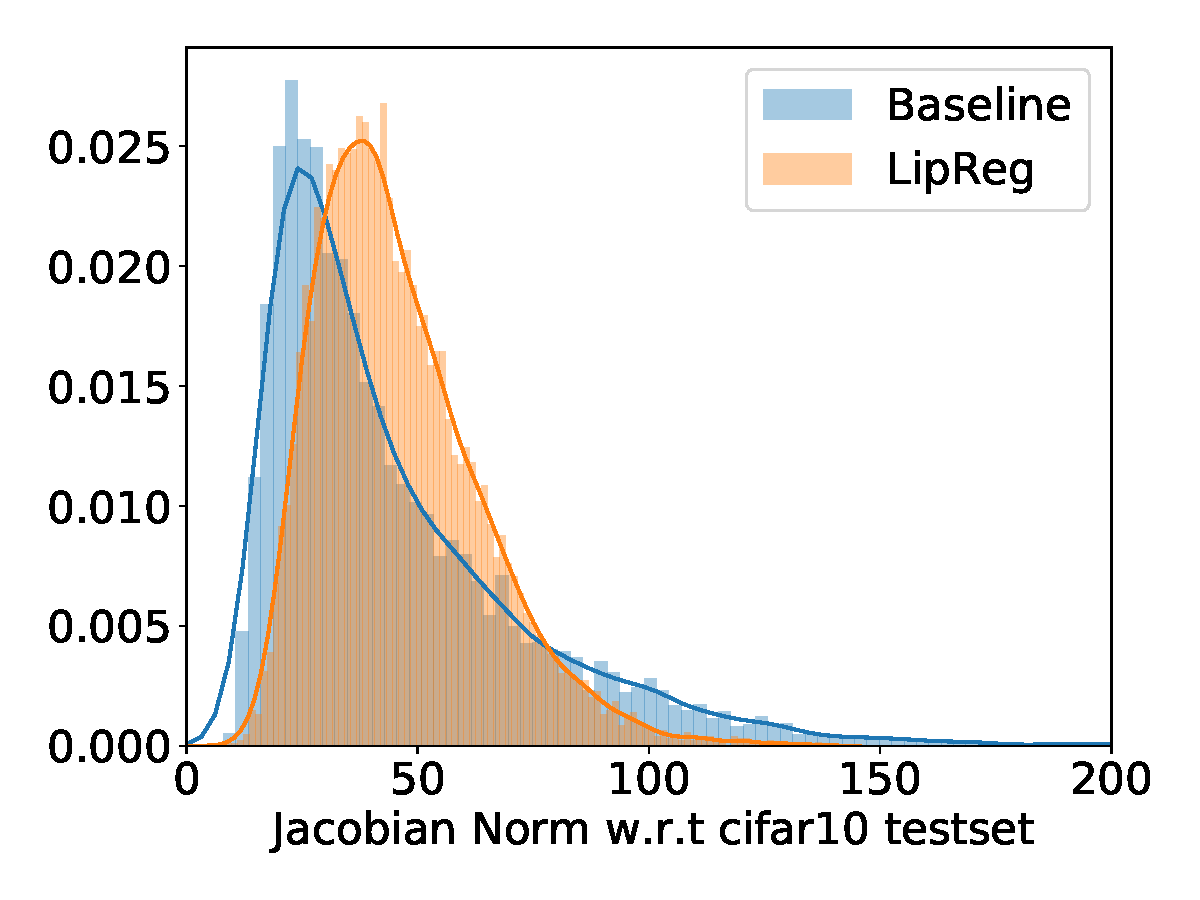
\includegraphics[width=\textwidth]{figures/chapter4/jacobian_distribution_v1.pdf}\\(a)
   \end{subfigure}
   \hfill
   \begin{subfigure}[b]{0.49\textwidth}
       \centering
       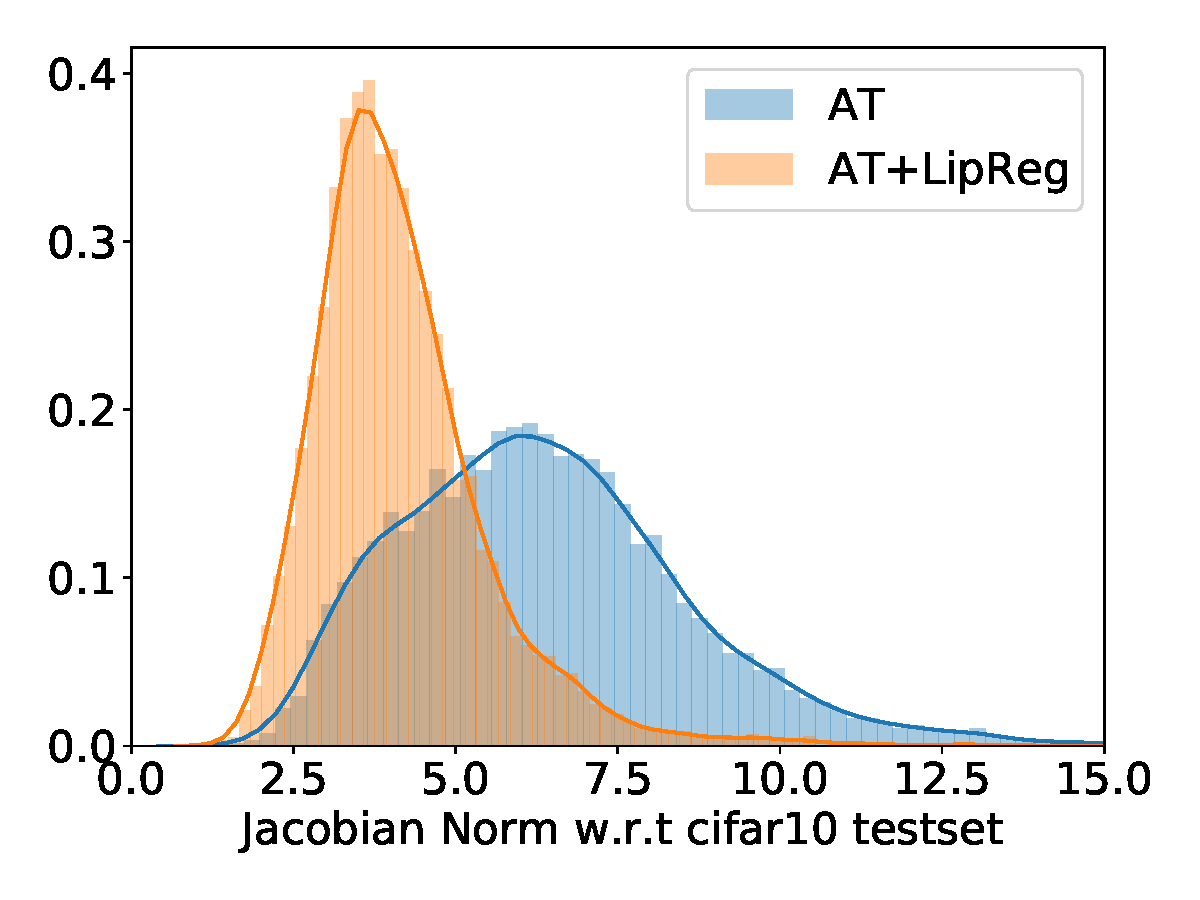
\includegraphics[width=\textwidth]{figures/chapter4/jacobian_distribution_v2.pdf}\\(b)
   \end{subfigure}
   \caption{These figures show the distribution of the norm of the Jacobian matrix w.r.t the CIFAR10 test set from a Wide Resnet trained with different schemes. Although Lipschitz regularization is not a Jacobian regularization, we can observe a clear shift in the distribution. This suggests that our method does not only work layer-wise, but also at the level of the entire network.}
   \label{figure:jacobian_distribution}
\end{figure}


\begin{figure}[ht]
   \centering
   \begin{subfigure}[b]{0.49\textwidth}
       \centering
       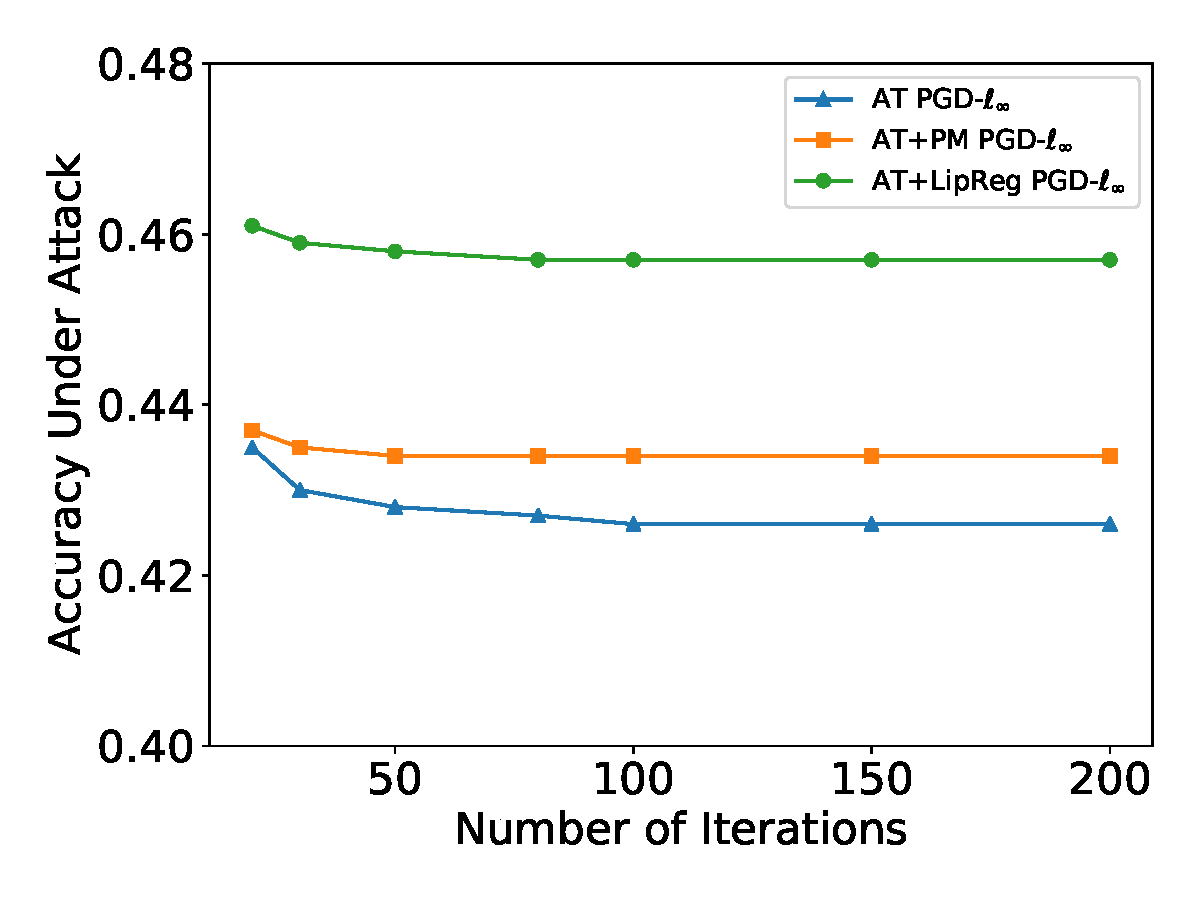
\includegraphics[width=\textwidth]{figures/chapter4/attacks_iter_pgd.pdf}\\(a)
   \end{subfigure}
   \hfill
   \begin{subfigure}[b]{0.49\textwidth}
       \centering
       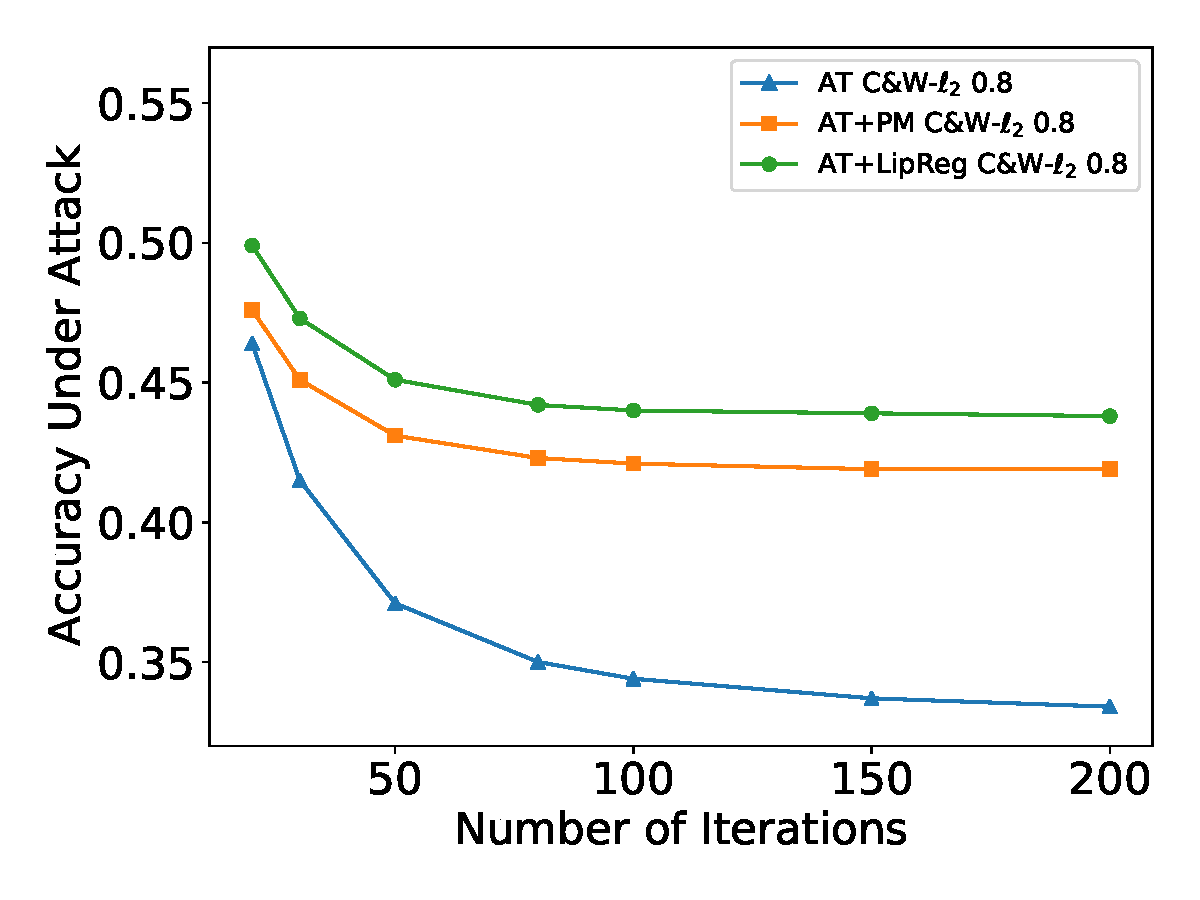
\includegraphics[width=\textwidth]{figures/chapter4/attacks_iter_cw.pdf}\\(b)
   \end{subfigure}
   \caption{These figures show the Accuracy under attack on CIFAR10 test set with PGD-$\linf$ and C\&W-$\ltwo$ attacks for several classifiers trained with Adversarial Training given the number of iterations.}
   \label{figure:attacks_iter}
\end{figure}


% \begin{figure*}[htb]
%   \centering
%   \begin{minipage}{.24\linewidth}
%     \centering
%     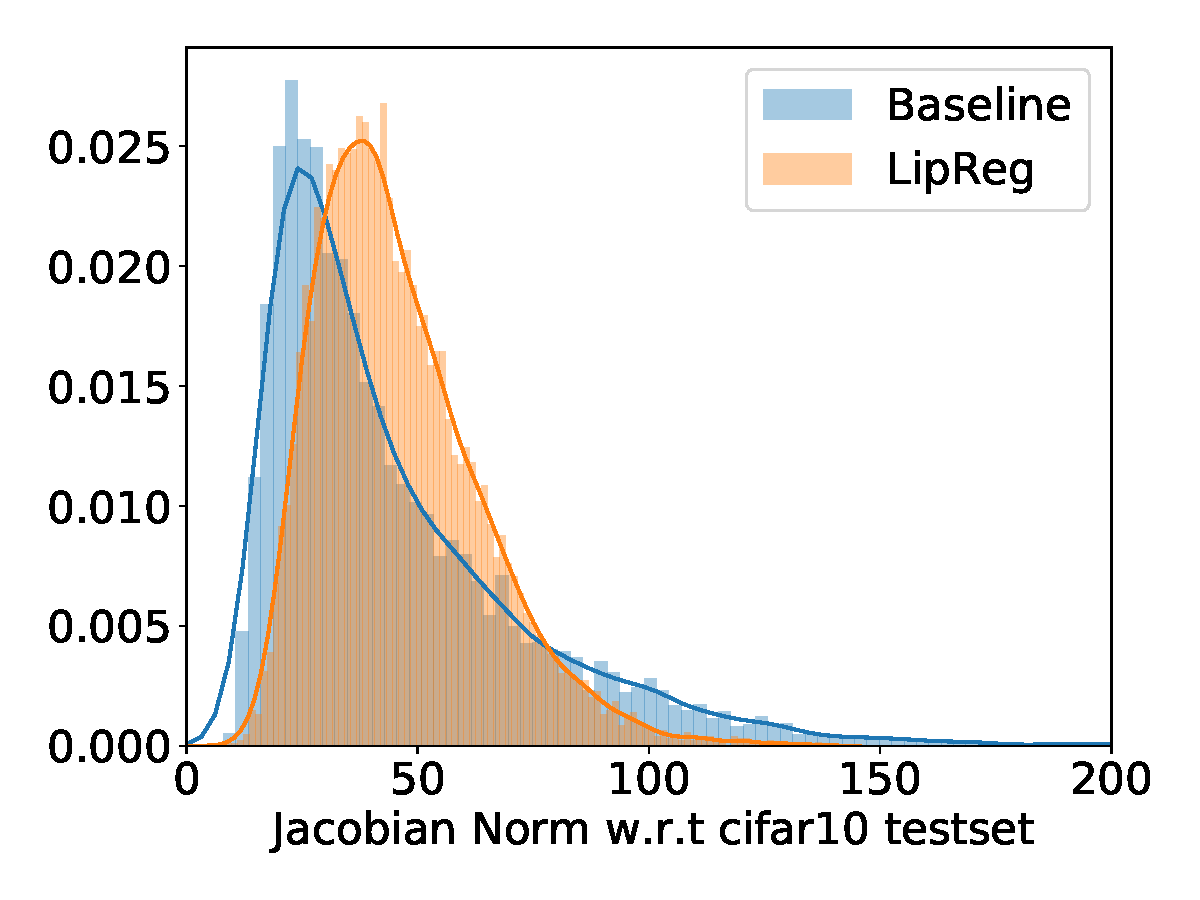
\includegraphics[scale=0.16]{figures/chapter4/jacobian_distribution_v1.pdf}\\{(a)}
%   \end{minipage}
%   \hfill
%   \begin{minipage}{.24\linewidth}
%     \centering
%     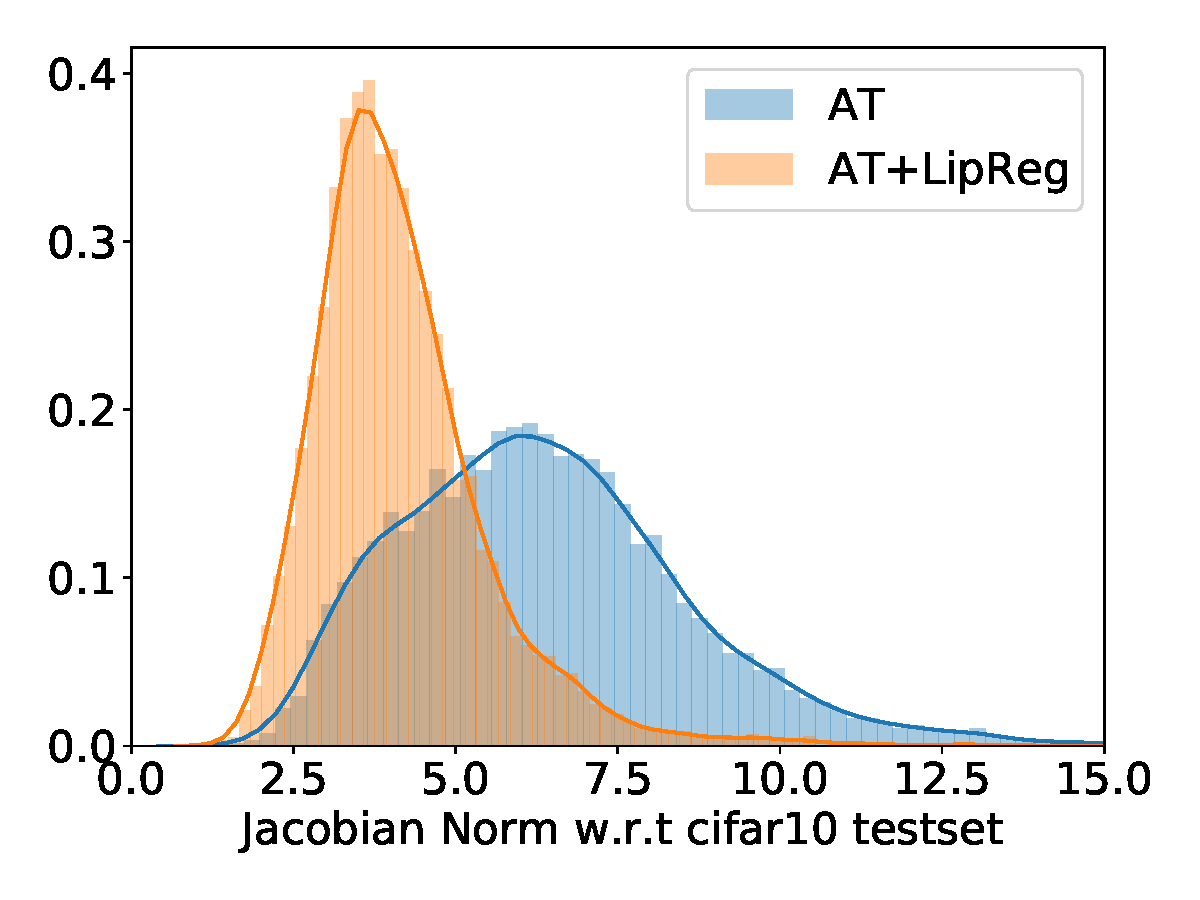
\includegraphics[scale=0.16]{figures/chapter4/jacobian_distribution_v2.pdf}\\{(b)}
%   \end{minipage}
%   \hfill
%   \begin{minipage}{.24\linewidth}
%     \centering
%     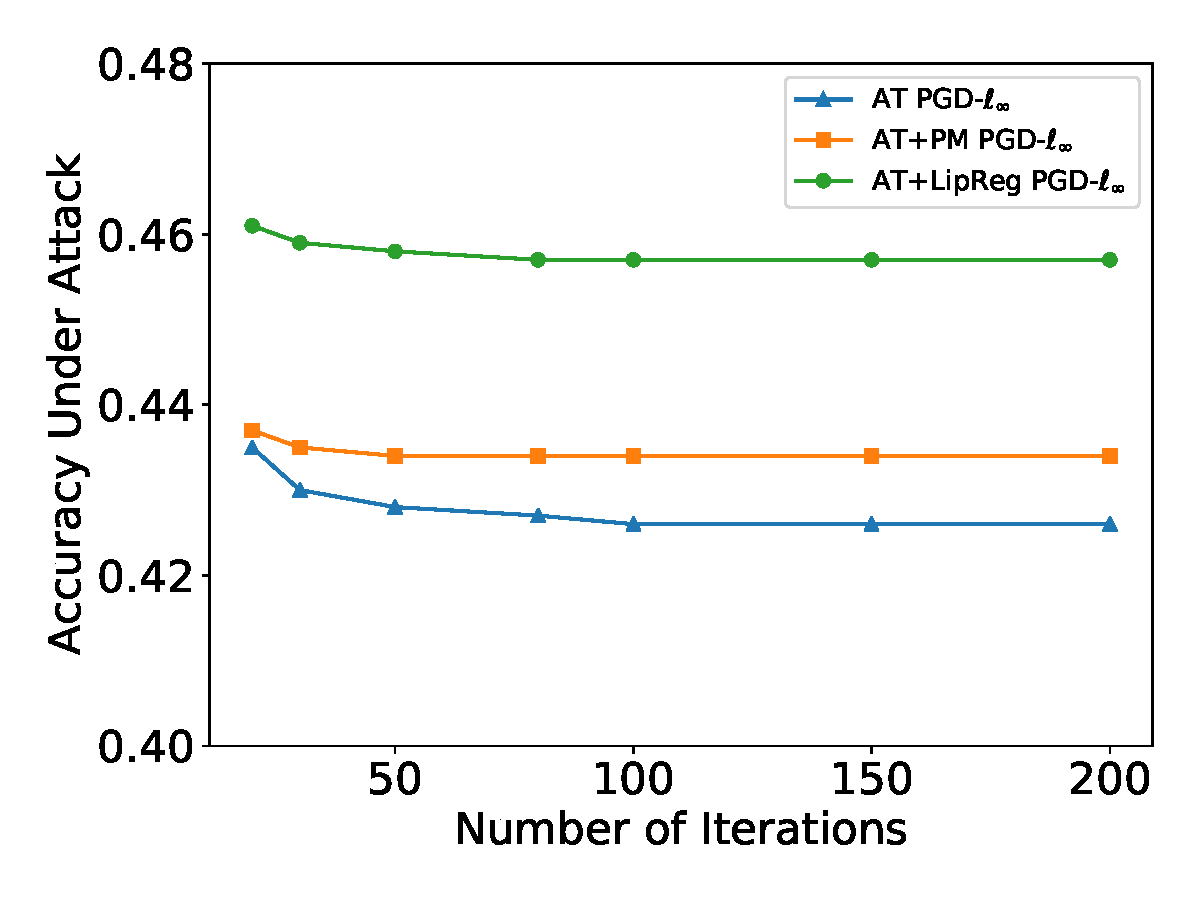
\includegraphics[scale=0.16]{figures/chapter4/attacks_iter_pgd.pdf}\\{(c)}
%   \end{minipage}
%   \hfill
%   \begin{minipage}{.24\linewidth}
%     \centering
%     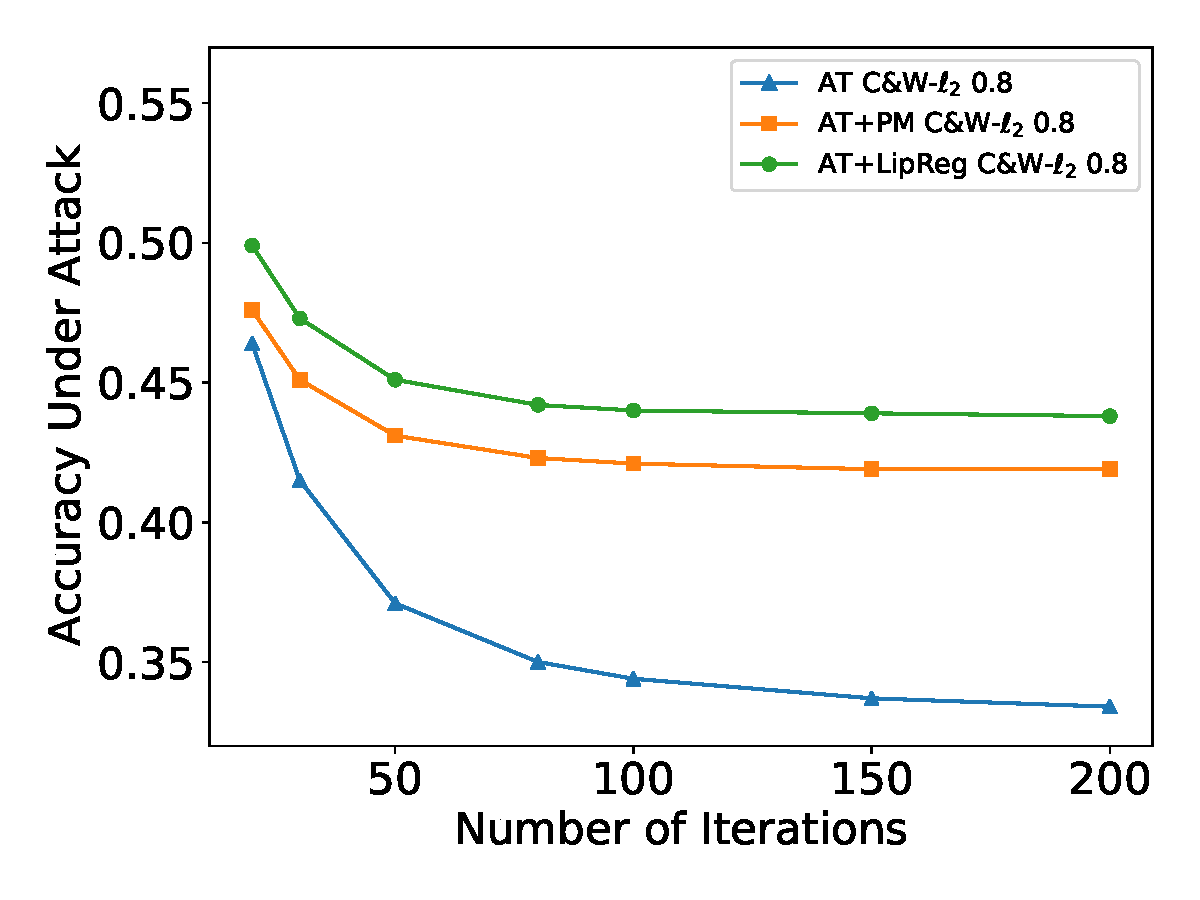
\includegraphics[scale=0.16]{figures/chapter4/attacks_iter_cw.pdf}\\{(d)}
%   \end{minipage}
%   \caption{Figures (a) and (b) show the distribution of the norm of the Jacobian matrix w.r.t the CIFAR10 test set from a Wide Resnet trained with different schemes. Although Lipschitz regularization is not a Jacobian regularization, we can observe a clear shift in the distribution. This suggests that our method does not only work layer-wise, but also at the level of the entire network. Figures (c) and (d) show the Accuracy under attack on CIFAR10 test set with PGD-$\linf$ and C\&W-$\ltwo$ attacks for several classifiers trained with Adversarial Training given the number of iterations.}
%   \label{figure:dist_jacobian_attacks_iter}
% \end{figure*}%


In this section, we compare the robustness of Adversarial Training~\cite{goodfellow2014explaining, madry2018towards} against the combination of Adversarial Training and Lipschitz regularization.
To regularize the Lipschitz constant of the network, we use the objective function defined in Equation~\ref{equation:objectif_function}.
We train Lipschitz regularized neural network with LipBound (Theorem~\ref{theorem:bound_max_sv_convolution}) implemented with PolyGrid (Algorithm~\ref{algorithm:PolyGrid}) (AT+LipBound) with $S = 10$ or with the specific power method for convolutions introduced by~\citet{farnia2018generalizable} with 10 iterations (AT+PM). 

Table~\ref{tab:table_cifar10_robustness} shows the gain in robustness against strong adversarial attacks.
We can observe that both AT+LipBound and AT+PM offer a better defense against adversarial attacks and that AT+LipBound offers a further improvement over the Power Method.
The Figure~\ref{figure:attacks_iter} (b) shows the Accuracy under attack with different number of iterations. 

Finally, we also conducted an experiment to study the impact of the regularization on the gradients of the whole network by measuring the norm of the Jacobian matrix, averaged over the inputs from the test set.
The results of this experiment are presented in Figure~\ref{figure:jacobian_distribution} (a) and show more concentrated gradients with Lipschitz regularization, which is the expected effect.
This suggests that our method does not only work layer-wise, but also at the level of the entire network.
A second experiment, using Adversarial Training, presented in Figure~\ref{figure:jacobian_distribution} (b) demonstrates that the effect is even stronger when the two techniques are combined together.
This corroborates the work by~\cite{farnia2018generalizable}.
It also demonstrates that Lipschitz regularization and Adversarial Training (or other Jacobian regularization techniques) are complementary.
Hence they offer an increased robustness to adversarial attacks as demonstrated above.

\paragraph{Experimental Settings}
We use the Wide ResNet architecture introduced by~\citet{ZagoruykoK16} to train our classifiers (for details of the hyper-parameters used, see the supplementary material).
For Adversarial Training ~\cite{madry2018towards}, we use Projected Gradient Descent with an $\epsilon = 8/255 (\approx 0.031)$, a step size of $\textstyle \frac{\epsilon}{5} (\approx 0.0062)$ and 10 iterations, we use a random initialization but run the attack only once.
To evaluate the robustness of our classifiers, we rigorously followed the experimental protocol proposed by~\citet{tramer2020adaptive} and~\citet{carlini2019evaluating}.
More precisely, as an $\linf$ attack, we use PGD with the same parameters ($\epsilon = 8/255$, a step size of $\textstyle \frac{\epsilon}{5}$) but we increase the number of iterations up to 200 with 10 restarts.
For each image, we select the perturbation that maximizes the loss among all the iterations and the 10 restarts.
As $\ltwo$ attacks, we use a bounded version of the~\cite{carlini2017towards} attack.
We choose $0.6$ and $0.8$ as bounds for the $\ltwo$ perturbation. Note that the $\ltwo$ ball with a radius of $0.8$ has approximately the same volume as the $\linf$ ball with a radius of $0.031$ for the dimensionality of CIFAR10. 


\subsection{Results on CIFAR100 dataset \& Hyper-parameters}

\begin{table}[htb]
  \centering
  \caption{This table shows the Accuracy under $\ltwo$ and $\linf$ attacks of CIFAR100 dataset. We compare Adversarial Training with the combination of Lipschitz regularization and Adversarial Training \cite{madry2018towards}. The $\lambda_2$ parameters which control the Lipschitz regularization is $0.008$, it has been chosen among a grid search of 10 values. The attacks below are computed with 200 iterations.}
    \begin{tabular}{lcccc}
    \toprule
      & \textbf{Accuracy} & \textbf{PGD-$\linf$} & \textbf{C\&W-$\ltwo$ 0.6} & \textbf{C\&W-$\ltwo$ 0.8} \\
    \midrule
    \textbf{Baseline} & $\mathbf{0.792}\pm0.000$ & $\phantom{.}0.000\pm0.000$ & $\phantom{.}0.001\pm0.000$ & $\phantom{.}0.000\pm0.000$ \\
    \textbf{AT} & \phantom{.}$0.591\pm0.000$ & $\phantom{.}0.199\pm0.000$ & $\phantom{.}0.263\pm0.000$ & $\phantom{.}0.183\pm0.000$ \\
    \textbf{AT+LipReg} & \phantom{.}$0.552\pm0.019$ & $\mathbf{0.215}\pm0.004$ & $\mathbf{0.294}\pm0.010$ & $\mathbf{0.226}\pm0.008$ \\
    \bottomrule
    \end{tabular}%
  \label{tab:results_cifar100}%
\end{table}%


\paragraph{Hyper-parameters used for training classifiers on CIFAR10 \& CIFAR100 dataset}
For all our experiments, we use the Wide Resnet architecture \cite{ZagoruykoK16} with 28 layers and a width factor of 10. We train our networks for 200 epochs with a batch size of $200$. We use Stochastic Gradient Descent with a momentum of $0.9$, an initial learning rate of $0.1$ with exponential decay of 0.1 (MultiStepLR gamma = 0.1) after the epochs $60$, $120$ and $160$. 

\subsection{Results on ImageNet dataset \& Hyper-parameters}

\begin{table}[htb]
  \centering
  \caption{This table shows the accuracy and accuracy under attack of ImageNet dataset with different training schemes. We compare Adversarial Training with the combination of Lipschitz regularization and Adversarial Training \cite{madry2018towards}. }
    {\footnotesize
    \begin{tabular}{lccccccccc}
    \toprule
      & \multicolumn{1}{c}{\multirow{2}[4]{*}{$\lambda_2$}} & \multicolumn{1}{c}{\multirow{2}[4]{*}{\textbf{Natural}}} &   & \multicolumn{2}{c}{\textbf{PGD-}$\linf$} &   & \multicolumn{3}{c}{\textbf{C\&W-}$\ltwo$} \\
\cmidrule{5-6}\cmidrule{8-10}      &   &   &   & \multicolumn{1}{c}{0.02} & \multicolumn{1}{c}{0.031} &   & \multicolumn{1}{c}{1.00} & \multicolumn{1}{c}{2.00} & \multicolumn{1}{c}{3.00} \\
    \midrule
    \textbf{AT} & \multicolumn{1}{c}{-} & 0.509 &   & 0.251 & 0.118 &   & 0.307 & 0.168 & 0.099 \\
    \textbf{AT+LipReg} & 0.0006 & \textbf{0.515} &   & \textbf{0.255} & \textbf{0.121} &   & \textbf{0.316} & \textbf{0.177} & \textbf{0.105} \\
    \textbf{AT+LipReg} & 0.0010 & \textbf{0.519} &   & \textbf{0.259} & \textbf{0.123} &   & \textbf{0.338} & \textbf{0.204} & \textbf{0.129} \\
    \bottomrule
    \end{tabular}%
    }
\end{table}%


\paragraph{Hyper-parameters used for training and attacking classifiers on ImageNet dataset}

For all our experiments, we use the Resnet-101 architecture \cite{He_2016_CVPR}.
We have used Stochastic Gradient Descent with a momentum of $0.9$, a weight decay of $0.0001$, label smoothing of $0.1$, an initial learning rate of $0.1$ with exponential decay of $0.1$ (MultiStepLR gamma = $0.1$) after the epochs $30$ and $60$.
We have used Exponential Moving Average over the weights with a decay of $0.999$.
We have trained our networks for 80 epochs with a batch size of $4096$.
For Adversarial Training, we have used PGD with 5 iterations, $\epsilon = 8/255 (\approx 0.031)$ and a step size of $\frac{\epsilon}{5} (\approx 0.0062)$. 

To evaluate the robustness of our classifiers in ImageNet, we have used an $\linf$ and an $\ltwo$ attacks. More precisely, as an $\linf$ attack, we use PGD with an epsilon of 0.02 and 0.031, a step size of $\textstyle \frac{\epsilon}{5}$) but we increase the number of iterations to 30 with 5 restarts. For each image, we select the perturbation that maximizes the loss among all the iterations and the 10 restarts. As $\ltwo$ attacks, we use a bounded version of the~\cite{carlini2017towards} attack. We have used $1$, $2$ and $3$ as bounds for the $\ltwo$ perturbation. 


%%%%%%%%%%%%%%%%%%%%%%%%%%%%%%%%%%%%%%%%%%%%%%%%%%%%%%%%%%%%%%%%%%%%%%%%%%%%%%%
\section{Conclusion}
\label{section:ch5-conclusion}
%%%%%%%%%%%%%%%%%%%%%%%%%%%%%%%%%%%%%%%%%%%%%%%%%%%%%%%%%%%%%%%%%%%%%%%%%%%%%%%

In this chapter, we introduced a new bound on the Lipschitz constant of convolutional layers that is both accurate and efficient to compute.
We used this bound to regularize the Lipschitz constant of neural networks and demonstrated its computational efficiency in training large neural networks with a regularized Lipschitz constant.
As an illustrative example, we   combined our bound with adversarial training, and showed that this increases the robustness of the trained networks to  adversarial attacks.
The scope of our results goes beyond this application and can be used  in a wide variety of settings, for example, to stabilize Generative Adversarial Networks, or improve generalization capabilities of classifiers, to mention a few.
Our future work will focus on investigating these fields. 





% \section{Additional Results and Discussions on the Experiments}
%
%
%
% \subsection{Additional Results and Discussion of Section~\ref{subsection:comparaison_sota}}
%
%
% \begin{table}[htb]
%   \centering
%   \caption{This table shows the efficiency of LipBound computation vs the Power Method with 10 iterations on the full networks.}
%   {\footnotesize
%     \begin{tabular}{llllr}
%     \toprule
%       &   & \multicolumn{1}{c}{\textbf{LipBound (ms)}} & \multicolumn{1}{c}{\textbf{Power Method (ms)}} & \textbf{Ratio} \\
%     \midrule
%      \cite{krizhevsky2012imagenet} & \textbf{AlexNet} & \phantom{....}$4.75\pm1.1$ & \phantom{....}$38.75\pm2.52$ & \textbf{8.14 }\\
%     \midrule
%     \multirow{5}[2]{*}{\cite{he2016deep}} & \textbf{ResNet 18} & \phantom{..}$29.88\pm1.73$ & \phantom{..}$148.35\pm14.92$ & \textbf{4.96 }\\
%       & \textbf{ResNet 34} & \phantom{..}$54.73\pm3.62$ & \phantom{..}$266.85\pm25.35$ & \textbf{4.87 }\\
%       & \textbf{ResNet 50} & \phantom{..}$60.77\pm4.62$ & \phantom{..}$467.61\pm36.52$ & \textbf{7.69 }\\
%       & \textbf{ResNet 101} & $102.72\pm11.53$ & \phantom{..}$817.06\pm102.87$ & \textbf{7.95 }\\
%       & \textbf{ResNet 152} & $158.80\pm20.84$ & $1373.57\pm164.37$ & \textbf{8.64} \\
%     \midrule
%     \multirow{4}[2]{*}{\cite{huang2017densely}} & \textbf{DenseNet 121} & $125.55\pm14.59$ & \phantom{..}$937.35\pm11.52$ & \textbf{7.46 }\\
%       & \textbf{DenseNet 161} & $176.11\pm19.13$ & $1292.61\pm30.5$ & \textbf{7.33} \\
%       & \textbf{DenseNet 169} & $188.03\pm19.74$ & $1372.62\pm21.16$ & \textbf{7.29} \\
%       & \textbf{DenseNet 201} & $281.13\pm23.41$ & $1930.19\pm170.79$ & \textbf{6.86 }\\
%     \midrule
%     \multirow{4}[2]{*}{\cite{simonyan2014very}} & \textbf{VGG 11} & \phantom{..}$13.73\pm1.19$ & \phantom{....}$81.78\pm4.45$ & \textbf{5.95 }\\
%       & \textbf{VGG 13} & \phantom{..}$14.96\pm1.99$ & \phantom{..}$102.04\pm4.2$ & \textbf{6.82 }\\
%       & \textbf{VGG 16} & \phantom{..}$21.92\pm1.94$ & \phantom{..}$132.29\pm5.99$ & \textbf{6.03 }\\
%       & \textbf{VGG 19} & \phantom{..}$29.05\pm0.66$ & \phantom{..}$162.28\pm4.87$ & \textbf{5.58 }\\
%     \midrule
%     \cite{ZagoruykoK16} & \textbf{WideResnet 50-2} & $113.28\pm45.44$ & \phantom{..}$468.74\pm6.54$ & \textbf{4.13 }\\
%     \midrule
%     \multirow{2}[2]{*}{\cite{iandola2016squeezenet}} & \textbf{SqueezeNet 1-0} & \phantom{..}$18.44\pm5.93$ & \phantom{....}$222.4\pm25.49$ & \textbf{12.05} \\
%       & \textbf{SqueezeNet 1-1} & \phantom{..}$18.26\pm6.65$ & \phantom{....}$209.8\pm3.59$ & \textbf{11.48} \\
%     \bottomrule
%     \end{tabular}%
%     }
%   \label{tab:efficiency_lipbound_full_model}%
% \end{table}%
%
% The comparison of Table~\ref{table:comparaison} of Section~\ref{subsection:comparaison_sota} of the main paper has been made with the following code provided by the authors: 
% \begin{itemize}
%     \item \makebox[3.2cm]{\cite{sedghi2018iclr}\hfill} \url{https://github.com/brain-research/conv-sv}
%     \item \makebox[3.2cm]{\cite{singla2019bounding}\hfill} \url{https://github.com/singlasahil14/CONV-SV}
%     \item \makebox[3.2cm]{\cite{farnia2018generalizable}\hfill} \url{https://github.com/jessemzhang/dl_spectral_normalization}
% \end{itemize}
% We translated the code of \cite{sedghi2018iclr} from TensorFlow to PyTorch in order to use the PyTorch CUDA Profiler.
%
% We extended the experiments presented in Table~\ref{table:comparaison} of Section~\ref{subsection:comparaison_sota} with Table~\ref{tab:efficiency_lipbound_full_model}.
% This table shows the efficiency of LipBound computation vs the Power Method with 10 iterations on the full network (\ie on all the convolutions of each network).
% The Ratio represents the \emph{speed gain} between our proposed method and the Power Method. 
%
% % \subsection{Additional Results of Section~\ref{section:experiments} \& Hyper-parameters}
%
%
% \subsection{The Effect of Lipschitz Regularization on the Maximal Singular Value of Convolution Layer}
%
% \begin{figure*}[htb]
%     \centering
%     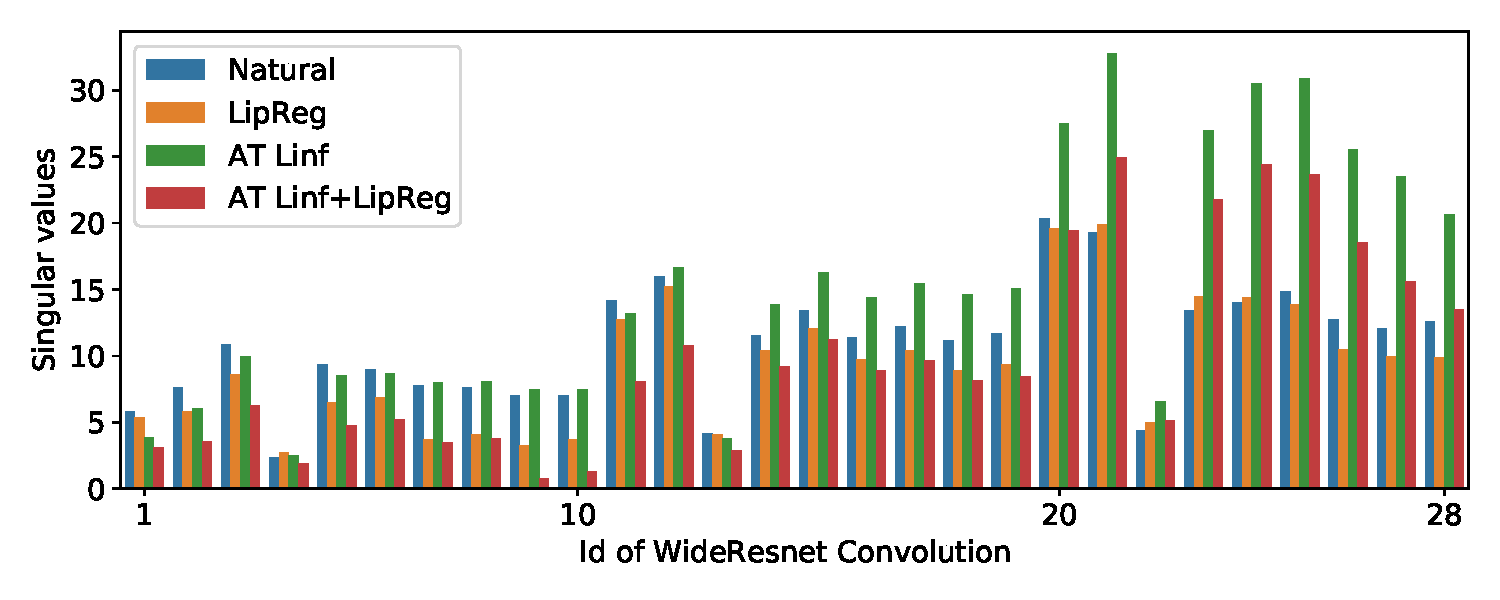
\includegraphics[scale=0.55]{figures/chapter4/singular_values.pdf}
%     \caption{This figure shows the maximal singular values of each convolution of a trained Wide ResNet on CIFAR10 dataset given different training scheme. The id 1 and 28 correspond to the first layer and last layer of the network.}
%     \label{figure:singular_values}
% \end{figure*}%
%
% Figure~\ref{figure:singular_values} shows the maximal singular values of each convolution of a trained Wide ResNet on CIFAR10 dataset given different training scheme. We can observe a small but clear decrease in the magnitude of the maximal singular values between Baseline and LipReg (blue and orange) on most of the convolution layers. A high increase of the maximal singular values appear with Adversarial Training. This is expected because the training scheme requires to the network to be a lot more expressive with the same number of parameters. We can observe that LipReg combined with AT have an important impact due on the singular value. 
%
%

  %%%%%%%%%%%%%%%%%%%%%%%%%%%%%%%%%%%%%%%%%%%%%%%%%%%%%%%%%%%%%%%%%%%%%%%%
\chapter{Conclusion}
\label{chapter:conlusion}
%%%%%%%%%%%%%%%%%%%%%%%%%%%%%%%%%%%%%%%%%%%%%%%%%%%%%%%%%%%%%%%%%%%%%%%%
\localtableofcontents

\todo{Write conclusion}


\section{Summary of the contributions}

xxx

\section{Discussion}

xxx


\section{Perspectives}

xxx


  \renewcommand\appendixpagename{\usekomafont{disposition}Appendices}
  \begin{appendices}
    \renewcommand\chaptername{Appendix}
    %%%%%%%%%%%%%%%%%%%%%%%%%%%%%%%%%%%%%%%%%%%%%%%%%%%%%%%%%%%%%%%%%%%%%%%%%%%%%%%
\chapter{Technical Proofs}
\label{chapter:technical_proofs}
%%%%%%%%%%%%%%%%%%%%%%%%%%%%%%%%%%%%%%%%%%%%%%%%%%%%%%%%%%%%%%%%%%%%%%%%%%%%%%%
\localtableofcontents

%%%%%%%%%%%%%%%%%%%%%%%%%%%%%%%%%%%%%%%%%%%%%%%%%%%%%%%%%%%%%%%%%%%%%%%%%%%%%%%
\section{Proofs of Chapter~\ref{chapter:diagonal_circulant_neural_network}}
%%%%%%%%%%%%%%%%%%%%%%%%%%%%%%%%%%%%%%%%%%%%%%%%%%%%%%%%%%%%%%%%%%%%%%%%%%%%%%%


\begin{proof}[\proofrefth{theorem:rank-decomposition}]
Let $\Umat \mathbf{\Sigma} \Vmat^{T}$ be the SVD decomposition of $\Mmat$ where $\Umat,\Vmat$ and $\mathbf{\Sigma}$ are $n \times n$ matrices.
Because $\Mmat$ is of rank $k$, the last $n-k$ columns of $\Umat$ and $\Vmat$ are null.
In the following, we will first decompose $\Umat$ into a product of matrices $\Wmat\Rmat\Omat$, where $\Rmat$ and $\Omat$ are respectively circulant and diagonal matrices, and $\Wmat$ is a matrix which will be further decomposed into a product of diagonal and circulant matrices.
Then, we will apply the same decomposition technique to $\Vmat$.
Ultimately, we will get a product of $4k+2$ matrices alternatively diagonal and circulant.  

Let $\Rmat = \circulant(r_{1}\ldots r_{n})$. Let $\Omat$ be a $n \times n$ diagonal matrix where $\Omat_{i,i} = 1$ if $i \le k$ and $0$ otherwise. The $k$ first columns of the product $\Rmat\Omat$ will be equal to that of $\Rmat$, and the $n-k$ last colomns of $\Rmat\Omat$ will be zeros. For example, if $k=2$, we have: 
\begin{equation}
  \Rmat\Omat = \leftmatrix
  r_{1} & r_{n} & 0 & \cdots & 0\\
  r_{2} & r_{1}\\
  r_{3} & r_{2} & \vdots &  & \vdots\\
  \vdots & \vdots\\
  r_{n} & r_{n-1} & 0 & \cdots & 0
  \rightmatrix
\end{equation}

Let us define $k$ diagonal matrices $\Dmat_{i} = \diagonal(d_{i1} \ldots d_{in})$ for $i \in [k]$.
For now, the values of $d_{ij}$ are unknown, but we will show how to compute them.
Let $\Wmat = \sum_{i=1}^{k} \Dmat_{i} \Smat^{i-1}$ where $\Smat$ is the \emph{cyclic shift} matrix 
%$S \in \mathbb{R}^{n\times n}$
define as follows:
\begin{equation}
  \Smat = \leftmatrix 0 &  &  &  & 1 \\
  1 & 0 \\
   & 1 & \ddots \\
   &  & \ddots & 0 \\
   &  &  & 1 & 0
  \rightmatrix
\end{equation}


Note that the $n-k$ last columns of the product $\Wmat\Rmat\Omat$ will be zeros.
For example, with $k=2$, we have: 
\begin{equation}
  \Wmat = \leftmatrix
  d_{1,1} &  &  &  & d_{2,1} \\
  d_{2,2} & d_{1,2} \\
   & d_{2,3} & \ddots \\
   &  & \ddots \\
   &  &  & d_{2,n} & d_{1,n}
  \rightmatrix
\end{equation}

\begin{equation}
  \Wmat\Rmat\Omat = \leftmatrix
  r_{1}d_{11}+r_{n}d_{21} & r_{n}d_{11}+r_{n-1}d_{21} & 0 & \cdots & 0 \\
  r_{2}d_{12}+r_{1}d_{22} & r_{1}d_{12}+r_{n}d_{22}\\
   &  & \vdots &  & \vdots \\
  \vdots & \vdots\\
  r_{n}d_{1n}+r_{n-1}d_{2n} & r_{n-1}d_{1n}+r_{n-2}d_{2n} & 0 & \cdots & 0
  \rightmatrix
\end{equation}
We want to find the values of $d_{ij}$ such that $\Wmat \Rmat \Omat = \Umat$. We can formulate this as linear equation system. In case $k=2$, we get:
\begin{equation}
  \leftmatrix
  r_{n} & r_{1}\\
  r_{n-1} & r_{n}\\
   &  & r_{1} & r_{2}\\
   &  & r_{n} & r_{1}\\
   &  &  &  & r_{2} & r_{3}\\
   &  &  &  & r_{1} & r_{2}\\
   &  &  &  &  &  & \ddots\\
   &  &  &  &  &  &  & \ddots
  \rightmatrix \times \leftmatrix
  d_{2,1}\\
  d_{1,1}\\
  d_{2,2}\\
  d_{1,2}\\
  d_{2,3}\\
  d_{1,3}\\
  \vdots\\
  \vdots
  \rightmatrix = \leftmatrix
  \Umat_{1,1}\\
  \Umat_{1,2}\\
  \Umat_{2,1}\\
  \Umat_{2,2}\\
  \\
  \\
  \vdots\\
  \\
  \rightmatrix
\end{equation}

The $i^{th}$ bloc of the bloc-diagonal matrix is a Toeplitz matrix induced by a subsequence of length $k$ of $(r_1,\ldots r_n,r_1 \ldots r_n)$.
Set $r_{j}=1$ for all $j\in\{k,2k,3k,\ldots n\}$ and set $r_{j}=0$ for all other values of $j$.
Then it is easy to see that each bloc is a permutation of the identity matrix.
Thus, all blocs are invertible.
This entails that the block diagonal matrix above is also invertible.
So by solving this set of linear equations, we find $d_{1,1}\ldots d_{k,n}$ such that $\Wmat\Rmat\Omat=\Umat$.
We can apply the same idea to factorize $\Vmat=\Wmat'.\Rmat.\Omat$ for some matrix $\Wmat'$.
Finally, we get 
\begin{equation}
  \Amat = \Umat \mathbf{\Sigma} \Vmat^\top = \Wmat\Rmat\Omat \mathbf{\Sigma} \Omat^\top \Rmat^\top \Wmat^{'\top}
\end{equation}

Thanks to Theorem~\ref{theorem:huhtanen}, $\Wmat$ and $\Wmat'$ can both be factorized in a product of $2k-1$ circulant and diagonal matrices.
Note that $\Omat \mathbf{\Sigma} \Omat^\top$ is diagonal, because all three are diagonal.
Overall, $\Amat$ can be represented with a product of $4k+2$ matrices, alternatively diagonal and circulant.
\end{proof}




%%%%%%%%%%%%%%%%%%%%%%%%%%%%%%%%%%%%%%%%%%%%%%%%%%%%%%%%%%%%%%%%%%%%%%%%%%%%%%%
\section{Proofs of Chapter~\ref{chapter:lipschitz_bound}}
%%%%%%%%%%%%%%%%%%%%%%%%%%%%%%%%%%%%%%%%%%%%%%%%%%%%%%%%%%%%%%%%%%%%%%%%%%%%%%%

\begin{proof}[\proofreflem{theorem:widom_idenity}]
Let $(i, j)$ be matrix indexes such $(\ \cdot\ )_{i, j}$ correspond to the value at the $i^\textrm{th}$ row and $j^\textrm{th}$ column, let us define the following notation:
\begin{align*}
    i_1 &= \left\lfloor i/n \right\rfloor \quad \quad &&j_1 = \left\lfloor j/n \right\rfloor \\
    i_2 &= i \mod n \quad \quad &&j_2 = j \mod n
\end{align*}

Let us define $\hat{f}$ as the 2 dimensional Fourier transform of the function $f$. We refer to $\hat{f}_{h_1, h_2}$ as the Fourier coefficient indexed by $(h_1, h_2)$ where $h_1$ correspond to the index of the block of the doubly-block Toeplitz and $h_2$ correspond to the index of the value inside the block. More precisely, we have 
\begin{align}
    \leftmat \Dmat(f) \rightmat_{i, j} &= \hat{f}_{(\left\lfloor j/n \right\rfloor - \left\lfloor i/n \right\rfloor), ((j \mod n) - (i \mod n)))} \label{equation:expression_fourier} \\
    \leftmat \Hmat^{\alpha_0}(f) \rightmat_{i, j} &= \hat{f}_{(\left\lfloor j/n \right\rfloor + \left\lfloor i/n \right\rfloor + 1), ((j \mod n) - (i \mod n)))} \\
    \leftmat \Hmat^{\alpha_1}(f) \rightmat_{i, j} &= \hat{f}_{(\left\lfloor j/n \right\rfloor - \left\lfloor i/n \right\rfloor), ((j \mod n) + (i \mod n) + 1))} \\
    \leftmat \Hmat^{\alpha_2}(f) \rightmat_{i, j} &= \hat{f}_{(\left\lfloor j/n \right\rfloor - \left\lfloor i/n \right\rfloor), ((j \mod n) - (i \mod n)))} \\
    \leftmat \Hmat^{\alpha_3}(f) \rightmat_{i, j} &= \hat{f}_{(\left\lfloor j/n \right\rfloor + \left\lfloor i/n \right\rfloor + n), ((j \mod n) + (i \mod n) + 1))}
\end{align}

We simplify the notation of the expressions above as follow:
\begin{align}
    \leftmat \Dmat(f) \rightmat_{i, j} &= \hat{f}_{(j_1 - i_1), (j_2 - i_2 )} \\
    \leftmat \Hmat^{\alpha_0}(f) \rightmat_{i, j} &= \hat{f}_{(j_1 + i_1 + 1), (j_2 - i_2 )} \\
    \leftmat \Hmat^{\alpha_1}(f) \rightmat_{i, j} &= \hat{f}_{(j_1 - i_1), (j_2 + i_2 + 1)} \\
    \leftmat \Hmat^{\alpha_2}(f) \rightmat_{i, j} &= \hat{f}_{(j_1 - i_1), (j_2 - i_2 )} \\
    \leftmat \Hmat^{\alpha_3}(f) \rightmat_{i, j} &= \hat{f}_{(j_1 + i_1 + n), (j_2 + i_2 + 1)}
\end{align}

The convolution theorem states that the Fourier transform of a product of two functions is the convolution of their Fourier coefficients. Therefore, one can observe that the entry $(i, j)$ of the matrix $\Dmat(f g)$ can be express as follows:

\begin{equation*}
    \leftmat \Dmat(f g) \rightmat_{i, j} = \sum_{k_1 = -2n + 1}^{2n-1} \sum_{k_2 = -2n + 1}^{2n-1} \hat{f}_{(k_1-i_1),(k_2-i_2)} \hat{g}_{(j_1-k_1),(j_2-k_2)}. 
\end{equation*}


By splitting the double sums and simplifying, we obtain:
\begin{align} \label{equation:split_double_sum}
\left( \Dmat(f g) \right)_{i, j} &= 
\sum_{k_1, k_2 \in P} \left(
\hat{f}_{(k_1-i_1),(k_2-i_2)} \hat{g}_{(j_1-k_1),(j_2-k_2)} +
\hat{f}_{(-k_1-i_1-1),(k_2-i_2)} \hat{g}_{(j_1+k_1+1),(j_2-k_2)} \right. \notag \\ &\quad+ \left.
\hat{f}_{(k_1-i_1),(-k_2-i_2-1)} \hat{g}_{(j_1-k_1),(j_2+k_2+1)} +
\hat{f}_{(-k_1-i_1-1),(-k_2-i_2-1)} \hat{g}_{(j_1+k_1+1),(j_2+k_2+1)} \right. \notag \\ &\quad+ \left.
\hat{f}_{(k_1-i_1+n),(-k_2-i_2-1)} \hat{g}_{(j_1-k_1-n),(j_2+k_2+1)} +
\hat{f}_{(k_1-i_1+n),(k_2-i_2)} \hat{g}_{(j_1-k_1-n),(j_2-k_2)} \right. \notag \\ &\quad+ \left.
\hat{f}_{(k_1-i_1),(k_2-i_2+n)} \hat{g}_{(j_1-k_1),(j_2-k_2-n)} +
\hat{f}_{(k_1-i_1+n),(k_2-i_2+n)} \hat{g}_{(j_1-k_1-n),(j_2-k_2-n)} \right. \notag \\ &\quad+ \left.
\hat{f}_{(-k_1-i_1-1),(k_2-i_2+n)} \hat{g}_{(j_1+k_1+1),(j_2-k_2-n)}  \right)
\end{align}
where $P = \{ (k_1, k_2)\ |\ k_1, k_2 \in \mathbb{N} \cup 0, 0 \leq k_1 \leq n-1,  0 \leq k_2 \leq n-1 \}$.


Furthermore, we can observe the following:
\begin{equation*}
    \leftmat \Dmat(f) \Dmat(g) \rightmat_{i, j} = \sum_{k = 0}^{n^2} \leftmat\Dmat(f)\rightmat_{i, k} \leftmat\Dmat(g)\rightmat_{k, j}  = \sum_{k_1, k_2 \in P} \hat{f}_{(k_1-i_1),(k_2-i_2)} \hat{g}_{(j_1-k_1),(j_2-k_2)}
\end{equation*}

{\allowdisplaybreaks
\begin{flalign*}
    % # H1_a_.T @ H1_b
    \leftmat \Hmat^{\alpha_1 \top}(f^*) \Hmat^{\alpha_1}(g) \rightmat_{i, j} &=  \sum_{k_1, k_2 \in P} \hat{f}^*_{(k_1+i_1+1),(i_2-k_2)} \hat{g}_{(j_1+k_1+1),(j_2-k_2)} \\
    &=  \sum_{k_1, k_2 \in P} \hat{f}_{(-k_1-i_1-1),(k_2-i_2)} \hat{g}_{(j_1+k_1+1),(j_2-k_2)} \\
    % # H2_a_.T @ H2_b
    \leftmat \Hmat^{\alpha_2 \top}(f^*) \Hmat^{\alpha_2}(g) \rightmat_{i, j} &=  \sum_{k_1, k_2 \in P} \hat{f}^*_{(i_1-k_1),(k_2+i_2+1)} \hat{g}_{(j_1-k_1),(j_2+k_2+1)} \\
    &=  \sum_{k_1, k_2 \in P} \hat{f}_{(k_1-i_1),(-k_2-i_2-1)} \hat{g}_{(j_1-k_1),(j_2+k_2+1)} \\
    % # H3_a_.T @ H3_b
    \leftmat \Hmat^{\alpha_3 \top}(f^*) \Hmat^{\alpha_3}(g) \rightmat_{i, j} &=  \sum_{k_1, k_2 \in P} \hat{f}^*_{(k_1+i_1+1),(k_2+i_2+1)} \hat{g}_{(j_1+k_1+1),(k_2+j_2+1)} \\
    &= \sum_{k_1, k_2 \in P} \hat{f}_{(-k_1-i_1-1),(-k_2-i_2-1)} \hat{g}_{(j_1+k_1+1),(k_2+j_2+1)} \\
    % # H4_a_.T @ H4_b
    \leftmat \Hmat^{\alpha_4 \top}(f^*) \Hmat^{\alpha_4}(g) \rightmat_{i, j} &= \sum_{k_1, k_2 \in P} \hat{f}^*_{(i_1-k_1-n),(k_2+i_2+1)} \hat{g}_{(j_1-k_1-n),(j_2+k_2+1)} \\
    &=  \sum_{k_1, k_2 \in P} \hat{f}_{(k_1-i_1+n),(-k_2-i_2-1)} \hat{g}_{(j_1-k_1-n),(j_2+k_2+1)} \\
\end{flalign*}
}
Let us define the matrix $\Qmat$ of size $n^2 \times n^2$ as the anti-identity matrix. We have the following:

{\allowdisplaybreaks
\begin{flalign*}
    % # Y @ H1_a.T @ H1_b_ @ Y
    \leftmat \Hmat^{\alpha_1 \top}(f) \Hmat^{\alpha_1}(g^*) \rightmat_{i, j} &= \sum_{k_1, k_2 \in P} \hat{f}_{(k_1+i_1+1),(i_2-k_2)} \hat{g}^*_{(j_1+k_1+1),(j_2-k_2)} \\
    &= \sum_{k_1, k_2 \in P} \hat{f}_{(k_1+i_1+1),(i_2-k_2)} \hat{g}_{(-j_1-k_1-1),(k_2-j_2)} \\
    \Leftrightarrow \leftmat \Qmat \Hmat^{\alpha_1 \top}(f) \Hmat^{\alpha_1}(g^*) \Qmat \rightmat_{i, j} &= \sum_{k_1, k_2 \in P} \hat{f}_{(k_1-i_1+n),(k_2-i_2)} \hat{g}_{(j_1-k_1-n),(j_2-k_2)} \\
    % # Y @ H2_a.T @ H2_b_ @ Y
    \leftmat \Hmat^{\alpha_2 \top}(f) \Hmat^{\alpha_2}(g^*) \rightmat_{i, j} &=  \sum_{k_1, k_2 \in P} \hat{f}_{(i_1-k_1),(k_2+i_2+1)} \hat{g}^*_{(j_1-k_1),(j_2+k_2+1)} \\
    &=  \sum_{k_1, k_2 \in P} \hat{f}_{(i_1-k_1),(k_2+i_2+1)} \hat{g}_{(k_1-j_1),(-j_2-k_2-1)} \\
    \Leftrightarrow \leftmat \Qmat \Hmat^{\alpha_2 \top}(f) \Hmat^{\alpha_2}(g^*) \Qmat \rightmat_{i, j} &=  \sum_{k_1, k_2 \in P} \hat{f}_{(k_1-i_1),(k_2-i_2+n)} \hat{g}_{(j_1-k_1),(j_2-k_2-n)} \\
    % # Y @ H3_a.T @ H3_b_ @ Y
    \leftmat \Hmat^{\alpha_3 \top}(f) \Hmat^{\alpha_3}(g^*) \rightmat_{i, j} &=  \sum_{k_1, k_2 \in P}  \hat{f}_{(k_1+i_1+1),(k_2+i_2+1)} \hat{g}^*_{(j_1+k_1+1),(k_2+j_2+1)} \\
    &=  \sum_{k_1, k_2 \in P} \hat{f}_{(k_1+i_1+1),(k_2+i_2+1)} \hat{g}_{(-j_1-k_1-1),(-k_2-j_2-1)} \\
    \Leftrightarrow \leftmat \Qmat \Hmat^{\alpha_3 \top}(f) \Hmat^{\alpha_3}(g^*) \Qmat \rightmat_{i, j} &=  \sum_{k_1, k_2 \in P} \hat{f}_{(k_1-i_1+n),(k_2-i_2+n)} \hat{g}_{(j_1-k_1-n),(-k_2+j_2-n)} \\
    % # Y @ H4_a.T @ H4_b_ @ Y
    \leftmat \Hmat^{\alpha_4 \top}(f) \Hmat^{\alpha_4}(g^*) \rightmat_{i, j} &=  \sum_{k_1, k_2 \in P}  \hat{f}_{(-k_1+i_1-n),(k_2+i_2+1)} \hat{g}^*_{(j_1-k_1-n),(j_2+k_2+1)} \\
    &= \sum_{k_1, k_2 \in P} \hat{f}_{(-k_1+i_1-n),(k_2+i_2+1)} \hat{g}_{(-j_1+k_1+n),(-j_2-k_2-1)} \\
    \Leftrightarrow \leftmat \Qmat \Hmat^{\alpha_4 \top}(f) \Hmat^{\alpha_4}(g^*) \Qmat \rightmat_{i, j} &= \sum_{k_1, k_2 \in P} \hat{f}_{(-k_1-i_1-1),(k_2-i_2+n)} \hat{g}_{(j_1+k_1+1),(j_2-k_2-n)}
\end{flalign*}
}

Now, we can observe from Equation~\ref{equation:split_double_sum} that:
\begin{equation}
    \Dmat(fg) = \Dmat(f)\Dmat(g) + \sum_{p=0}^3 \Hmat^{\alpha_p \top}(f^*) \Hmat^{\alpha_p}(g) + \Qmat \left( \sum_{p=0}^3 \Hmat^{\alpha_p \top}(f) \Hmat^{\alpha_p}(g^*) \right) \Qmat.
\end{equation}
which concludes the proof. 
\end{proof}

    %%%%%%%%%%%%%%%%%%%%%%%%%%%%%%%%%%%%%%%%%%%%%%%%%%%%%%%%%%%%%%%%%%%%%%%%%%%%%%%
\chapter{Training compact deep learning models for video classification using circulant matrices}
\label{chapter:training_compact_deep_learning_models_for_video_classification_using_circulant_matrices}
%%%%%%%%%%%%%%%%%%%%%%%%%%%%%%%%%%%%%%%%%%%%%%%%%%%%%%%%%%%%%%%%%%%%%%%%%%%%%%%
\localtableofcontents

\todo{write context}
\emph{This work ..}



%%%%%%%%%%%%%%%%%%%%%%%%%%%%%%%%%%%%%%%%%%%%%%%%%%%%%%%%%%%%%%%%%%%%%%%%%%%%%%%
\section{Introduction}
\label{section:ap2-intro}
%%%%%%%%%%%%%%%%%%%%%%%%%%%%%%%%%%%%%%%%%%%%%%%%%%%%%%%%%%%%%%%%%%%%%%%%%%%%%%%

The top-3 most accurate approaches proposed during the first \yt\footnote{https://www.kaggle.com/c/youtube8m} video classification challenge  were all ensembles models.
The ensembles typically combined models based on a variety of deep learning architectures such as \emph{NetVLAD}, \emph{Deep Bag-of-Frames} (DBoF), \emph{NetFisherVectors} (NetFV) and \emph{Long-Short Term Memory} (LSTM), leading to a large aggregation of models (25 distinct models have been used by the first contestant~\cite{miech2017learnable}, 74 by the second~\cite{DBLP:journals/corr/WangZW17} and 57 by the third~\cite{DBLP:journals/corr/LiGLBLLLZW17}).
Ensembles are accurate, but they are not ideal: their size makes them difficult to maintain and deploy, especially on mobile devices. 

A common approach to compress large models into smaller ones is to use \emph{model distillation}~\cite{44873}.
Model distillation is a two steps training procedure: first, a large model (or an ensemble model) is trained to be as accurate as possible.
Then, a second compact model is trained to approximate the first one, while satisfying the given size constraints.
The success of model distillation and other model compression techniques begs an important question: is it possible to devise models that are compact by nature while exhibiting the same generalization properties as large ones?

In linear algebra, it is common to exploit structural properties of matrices to reduce the memory footprint of an algorithm. 
\citet{cheng} have used this principle in the context of deep neural networks to design compact network architectures by imposing a structure on weight matrices of fully connected layers.
They were able to replace large, unstructured weight matrices with structured \emph{circulant matrices} without significantly impacting the accuracy.
And because a n-by-n circulant matrix is fully determined by a vector of dimension $n$, they were able to train a neural network using only a fraction of the memory required to train the original network.

Inspired by this result, we designed several compact neural network architectures for video classification based on standard video architectures such as NetVLAD, DBoF, NetFV and we evaluated them on the large \yt dataset.
However, instead of adopting the structure used by \cite{cheng} (initially proposed by \cite{VYBIRAL20111096}), we decomposed weight matrices into products of diagonal and circulant matrices (as in \cite{schmid2000decomposing}).
In contrast with \cite{VYBIRAL20111096} which has been proved to approximate distance preserving projections, this structure can approximate \emph{any} transformation (at the cost of a larger number of weights).
As we will show, this approach exhibits good results on the video classification task at hand. 

In this paper, we bring the following contributions:

\begin{itemize}
  \item We define a compact architecture for video classification based on circulant matrices.
  As a side contribution, we also propose a new pooling technique which improves the Deep Bag-of-Frames embedding. 
  \item We conduct thorough experimentations to identify the layers that are less impacted by the use of circulant matrices and we fine-tune our architectures to achieve the best trade-off between size and accuracy.  
  \item We combine several architectures into a single model to achieve a new model trained-end-to-end that can benefit from architectural diversity (as in ensembles).
  \item We train all our models on the Youtube-8M dataset with the 1GB model size constraint imposed by the \emph{2nd YouTube-8M Video Understanding Challenge}\footnote{https://www.kaggle.com/c/youtube8m-2018}, and compare the different models in terms of size \vs accuracy ratio.
  Our experiments demonstrate that the best trade-off between size and accuracy is obtained using circulant DBoF embedding layer.
\end{itemize}

%%%%%%%%%%%%%%%%%%%%%%%%%%%%%%%%%%%%%%%%%%%%%%%%%%%%%%%%%%%%%%%%%%%%%%%%%%%%%%%
\section{Related Works}
\label{section:ap2-related-work}
%%%%%%%%%%%%%%%%%%%%%%%%%%%%%%%%%%%%%%%%%%%%%%%%%%%%%%%%%%%%%%%%%%%%%%%%%%%%%%%

Classification of unlabeled videos streams is one of the challenging tasks for machine learning algorithms.
Research in this field has been stimulated by the recent release of several large annotated video datasets such as \emph{Sports-1M}~\cite{karpathy2014large}, \emph{FCVID}~\cite{FCVID} or the \yt~\cite{abu2016youtube} dataset.

The naive approach to achieve video classification is to perform frame-by-frame image recognition, and to average the results before the classification step.
However, it has been shown in \cite{abu2016youtube,miech2017learnable} that  better results can be obtained by building features across different frames and several deep learning architectures have been designed to learn embeddings for sets of frames (and not single frames).
For example Deep Bag-of-Frames ~(DBoF)~\cite{abu2016youtube}, NetVLAD~\cite{Arandjelovic16} or architectures based on Fisher Vectors~\cite{4270291}. 


The DBoF embedding layer, proposed in~\cite{abu2016youtube} processes videos in two steps. 
First, a learned transformation projects all the frames together into a high dimensional space. 
Then, a max (or average) pooling operation aggregates all the embedded frames into a single discriminative vector  representation of the video.
The NetVLAD~\cite{Arandjelovic16} embedding layer is built on \emph{VLAD}~\cite{jegou:inria-00548637}, a technique that aggregates a large number of local frame descriptors into a compact representation using a codebook of visual words.
In NetVlad, the codebook is directly learned end-to-end during training.
Finally, NetFisherVector (NetFV) is inspired by~\cite{4270291} and uses  first and second-order statistics as video descriptors also gathered in a codebook.
The technique can benefit from deep learning by using a deep neural network to learn the codebook \cite{miech2017learnable}.

All the architectures mentioned above can be used to build video features in the sense of features that span across several frames, but they are not designed to exploit the sequential nature of videos and capture motion.
In order to learn truly spatio-temporal features and account for motion in videos, several researchers have looked into recurrent neural networks (\eg LSTM~\cite{yue2015beyond,DBLP:journals/corr/LiGLBLLLZW17}) and 3D convolutions~\cite{karpathy2014large} (in space and time).
However, these approaches do not  outperform non-sequential models, and  the single best model proposed in~\cite{miech2017learnable} (winner of the first \yt competition) is based on NetVLAD~\cite{Arandjelovic16}. 

The \emph{2nd YouTube-8M Video Understanding Challenge} includes a constraint on the model size and many competitors have been looking into building efficient memory models with high accuracy.
There are two kinds of techniques to reduce the memory required for training and/or inference in neural networks.
The first kind aims at \emph{compressing} an existing neural network into a smaller one, (thus it only impacts the size of the model at inference time).
The second one aims at \emph{constructing models that are compact} by design. 

To compress an existing network several researchers have investigated techniques to prune parameters that are redundant (\eg ~\cite{pmlr-v80-dai18d,han2015deep_compression,NIPS2017_6813}).
Redundant parameters can be omitted from the model without significantly changing the accuracy.
It is also possible to use sparsity regularizers during training, to be able to compress the model after the training using efficient sparse matrix representations (\eg~\cite{Collins2014MemoryBD,pmlr-v80-dai18d,7298681}).
Building on the observation that weight matrices are often redundant, another line of research has proposed to use matrix factorization~\cite{NIPS2013_5025,Jaderberg2014SpeedingUC,8099498} in order to decompose large weight matrices into factors of smaller matrices before inference.

An important idea in model compression, proposed by~\citet{bucilua2006model}, is based on the observation that the model used for training is not required to be the same as the one used for inference.
First, a large complex model is trained using all the available data and resources  to be as accurate as possible, then a smaller and more compact model is trained to approximate the first model.
The technique which was later specialized for deep learning models by~\citet{44873} (\aka model distillation) is often used to compress large ensemble models into compact single deep learning models.

Instead of compressing the model after the training step, one can try to design models that are compact by nature (without compromising the generalization properties of the network).
The benefit of this approach is that it reduces memory usage required during both training and inference.
As a consequence, users can train models that are virtually larger using less time and less computing resources.
They also save the trouble of training two models instead of one as it is done with distillation.
These techniques generally work by constraining the weight representation, either at the level of individual weights (\eg using floating variable with limited precision \cite{Gupta:2015:DLL:3045118.3045303}, quantization \cite{Courbariaux:2015:BTD:2969442.2969588,DBLP:journals/corr/MellempudiKM0KD17,rastegariECCV16}) or  at the level of the whole matrix, (\eg using weight hashing techniques~\cite{Chen:2015:CNN:3045118.3045361}) which can achieve better compression ratio.
However in practice, hashing techniques are difficult to use because of their irregular memory access patterns which makes them inadequate for GPU-execution.

Another way of constraining the weight representation is to impose a structure on weight matrices (\eg using circulant matrices~\cite{cheng,NIPS2015_5869}, Vandermonde~\cite{NIPS2015_5869} or Fastfood transforms~\cite{7410530}).
In this domain, \citet{cheng} have proposed to replace two fully connected layers of AlexNet by circulant and diagonal matrices where the circulant matrix is learned by a gradient based optimization algorithm and the diagonal matrix entries are sampled at random in $\{-1, 1\}$. 
The size of the model is reduced by a factor of 10 without loss in accuracy\footnote{In network such as AlexNet, the last 3 fully connected layers use 58M out of the 62M total trainable parameters ($> 90\%$ of the total number of parameters).}.
Most of the time the resulting algorithms are easy to execute on GPU-devices. 

%%%%%%%%%%%%%%%%%%%%%%%%%%%%%%%%%%%%%%%%%%%%%%%%%%%%%%%%%%%%%%%%%%%%%%%%%%%%%%%
\section{Preliminaries on circulant matrices}
\label{section:ap2-circ}
%%%%%%%%%%%%%%%%%%%%%%%%%%%%%%%%%%%%%%%%%%%%%%%%%%%%%%%%%%%%%%%%%%%%%%%%%%%%%%%

In this paper, we use \emph{circulant matrices} to build compact deep neural networks.
A n-by-n circulant matrix $C$ is a matrix where each row is a cyclic right shift of the previous one as illustrated below.

% \begin{equation*}\setlength\arraycolsep{1.5pt}
% C = circ(c) =\left[\begin{array}{C{2em}C{2em}C{2em}C{2em}C{2em}}
% $c_{0}$ & $c_{n-1}$ & $c_{n-2}$ & \dots & $c_{1}$ \\
% $c_{1}$ & $c_{0}$ & $c_{n-1}$ & & $c_{2}$ \\
% $c_{2}$ & $c_{1}$ & $c_{0}$ & & $c_{3}$ \\
% $\vdots$ & & & $\ddots$ & $\vdots$ \\
% $c_{n-1}$ & $c_{n-2}$ & $c_{n-3}$ & & $c_{0}$
% \end{array}\right]%
% \end{equation*}

% \[
%   C = circ(c) =\left[\begin{array}{ccccc}
%   c_{0} & c_{n-1} & c_{n-2} & \dots & c_{1} \\
%   c_{1} & c_{0} & c_{n-1} & & c_{2} \\
%   c_{2} & c_{1} & c_{0}& & c_{3} \\
%   \vdots & & & \ddots & \vdots \\
%   c_{n-1} & c_{n-2} & c_{n-3} & & \phantom{0}c_{0}\phantom{0}
%   \end{array}\right]
% \]

\begin{equation}
    \Cmat = \circulant(\cvec) = \leftmatrix
    c_{0} & c_{n-1} & c_{n-2} & \dots & c_{1} \\
    c_{1} & c_{0} & c_{n-1} & & c_{2} \\
    c_{2} & c_{1} & c_{0}& & c_{3} \\
    \vdots & & & \ddots & \vdots \\
    c_{n-1} & c_{n-2} & c_{n-3} & & \phantom{0}c_{0}\phantom{0}
    \rightmatrix
\end{equation}

Because the circulant matrix $C \in \Rbb^{n\times n}$ is fully determined by the vector $c \in \Rbb^n$, the matrix $C$ can be compactly represented in memory using only $n$ real values instead of $n^2$.

An additional benefit of circulant matrices, is that they are computationally efficient, especially on GPU devices.
Multiplying a circulant matrix $C$ by a vector $x$ is equivalent to a circular convolution between $c$ and $x$ (denoted $c \star x$).
Furthermore, the circular convolution can be computed in the Fourier domain as follows. 

\begin{equation}
  Cx \quad = \quad c \star x \quad = \quad \F^{-1}\left(\F(c) \times \F(x)\right)
\end{equation}
where $\F$ is the Fourier transform.
Because this operation can be simplified to a simple element wise vector multiplication, the matrix multiplication $Cx$ can be computed in $O(n \log n)$ instead of $O(n^2)$.

Among the many applications of circulant matrices, matrix decomposition is one of the interest.
\todo{correct ref bellow}
In particular, Schmid et al. have shown in \cite{muller1998algorithmic,schmid2000decomposing}, that any complex matrix $A \in \Cbb^{n\times n}$ can be decomposed into the product of diagonal and circulant matrices, as follows: 

\begin{equation}
  A = D^{(1)} C^{(1)} D^{(2)} C^{(2)} \dots D^{(m)} C^{(m)} = \prod_{i=1}^{m} D^{(i)} C^{(i)}
  \label{equation:ap2-general_framework}
\end{equation}

Later in \cite{Huhtanen2015}, Huhtanen and Perämäki have demonstrated that choosing $m=n$ is sufficient to decompose any complex matrix $A \in \Cbb^{n\times n}$.
By~\citet{schmid2000decomposing}, the result in Equation~\ref{equation:ap2-general_framework} also holds for a real matrix $A \in \Rbb^{n\times n}$, but the proof yields a much bigger value of $m$.
However,  the construction of \cite{schmid2000decomposing} is far from optimal and it is likely that most real matrices can be decomposed into a reasonable number of factors.
The authors of~\cite{moczulski2015acdc} made this conjecture, and they have leveraged the decomposition described in Equation~\ref{equation:ap2-general_framework} in order to implement compact fully connected layers.

%%%%%%%%%%%%%%%%%%%%%%%%%%%%%%%%%%%%%%%%%%%%%%%%%%%%%%%%%%%%%%%%%%%%%%%%%%%%%%%
\section{Compact  video classification architecture using circulant matrices}
\label{section:archi}
%%%%%%%%%%%%%%%%%%%%%%%%%%%%%%%%%%%%%%%%%%%%%%%%%%%%%%%%%%%%%%%%%%%%%%%%%%%%%%%

Building on the decomposition presented in the previous section and the previous results obtained in~\cite{moczulski2015acdc}, we now introduce a compact neural network architecture for video classification where dense matrices have been replaced by products of circulant and diagonal matrices.

%%%%%%%%%%%%%%%%%%%%%%%%%%%%%%%%%%%%%%%%%%%%%%%%%%%%%%%%%%%%%%%%%%%%%%%%%%%%%%%
\subsection{Base Model}
%%%%%%%%%%%%%%%%%%%%%%%%%%%%%%%%%%%%%%%%%%%%%%%%%%%%%%%%%%%%%%%%%%%%%%%%%%%%%%%

We demonstrate the benefit of circulant matrices using a base model which has been proposed by~\citet{miech2017learnable}.
This architecture can be decomposed into three blocks of layers, as illustrated in Figure~\ref{figure:ap2-model_baseline}. 
\begin{figure}[htb]
  \centering
  \tikzset{%
  >={Latex[width=2mm,length=2mm]},
  % Specifications for style of nodes:
            base/.style = {rectangle, draw=black, text centered, font=\sffamily},
             box/.style = {base, rounded corners, text depth=3cm, minimum height=4cm, minimum width=3cm},
     transparent/.style = {rectangle, draw=black},
       circulant/.style = {base, fill=yellow!30},
       embedding/.style = {base, fill=blue!30, minimum width=2.5cm, minimum height=1cm},
           other/.style = {base, fill=white!30,  minimum width=2cm, minimum height=1cm},
              fc/.style = {base, fill=orange!30, minimum width=1.5cm, minimum height=1cm},
          gating/.style = {base, fill=green!30, minimum width=2cm, text width=2cm, minimum height=1cm},
             moe/.style = {base, fill=purple!30, minimum width=1.5cm, minimum height=1cm},
}

\begin{tikzpicture}[every node/.style={fill=white, font=\sffamily}, align=center]

  \draw (0.0, +2.)  node [other, draw=none] {\textbf{Embedding}};
  \draw (+3.7, +2.)  node [other, draw=none] {\textbf{Dim Reduction}};
  \draw (+8.0, +2.)  node [other, draw=none] {\textbf{Classification}};

  \draw (0, +0.8)  node [embedding] {Video};
  \draw (0, -0.8)  node [embedding] {Audio};

  \draw (+2.5, +0.8)  node (fc) [fc] {FC};
  \draw (+2.5, -0.8)  node (fc) [fc] {FC};

  \draw (+4.75, 0)  node (fc) [other] {concat};
  \draw (+7.0, 0)  node (moe) [moe] {MoE};
  \draw (+9.25, 0)  node (gating2) [gating] {Context Gating};
 
  \draw (+1.5, +2) [dashed] -- (+1.5, -1.7);
  \draw (+6, +2) [dashed] -- (+6, -1.7);
  
\end{tikzpicture}
  \caption{This figure shows the architecture used for the experiences. The network samples at random video and audio frames from the input. The sample goes through an embedding layer and is reduced with a Fully Connected layer. The results are then concatenated and classified with a Mixture-of-Experts and Context Gating layer.}
  \label{figure:ap2-model_baseline}
\end{figure}

The first block of layers, composed of the Deep Bag-of-Frames embedding, is meant to process audio and video frames independently.
The DBoF layer computes two embeddings: one for the audio and one for the video.
In the next paragraph, we will only focus on describing the video embedding (The audio embedding is computed in a very similar way).

We represent a video $V$ as a set of $m$ frames $\{v_{1},\ldots,v_{m}\}$ where each frame $v_i \in \mathbb R^k$ is a vector of visual features extracted from the frame image.
In the context of the \yt competition, each $v_i$ is a vector of 1024 visual features extracted using the last fully connected layer of an Inception network trained on ImageNet.
The DBoF layer then embeds a video $V$ into a vector $v'$ drawn from a $p$ dimensional vector space as follows:

\begin{equation}
  v' = \max \left\{Wv_{i}\mid v_i \in V \right\}
\end{equation}
where $W$ is a matrix in $\Rbb^{p \times k}$ (learned) and max is the element-wise maximum operator.
We typically choose $p > k$, (\eg $p = 8192$).
Note that because this formulation is framed in term of sets, it can process videos of different lengths (\ie, a different value of $m$).

A second block of layers reduces the dimensionality of each embedding layer (audio and video), and merges the result into a single vector by using a simple concatenation operation.
We chose to reduce the dimensionality of each embedding layer separately \emph{before} the concatenation operation to avoid the concatenation of two high dimensional vectors.

Finally, the classification block uses a combination of Mixtures-of-Experts (MoE) and Context Gating to calculate the final probabilities.
The Mixtures-of-Experts layer introduced in~\cite{716791} and proposed for video classification in~\cite{abu2016youtube} is used to predict each label independently.
It consists of a gating and experts networks which are concurrently learned.
The gating network learns which experts to use for each label and the experts layers learn how to classify each label.
The context gating operation was introduced in~\cite{miech2017learnable} and captures dependencies among features and re-weight probabilities based on the correlation of the labels.
For example, it can capture the correlation of the labels \emph{ski} and \emph{snow} and re-adjust the probabilities accordingly. 

Table~\ref{table:ap2-shape_dbof} shows the shapes of the layers as well as the shapes of the weight matrices. 
\begin{table}[htb]
  \centering
  \caption{This table shows the architecture of our base model with a DBoF Embedding and 150 frames sampled from the input. For more clarity, weights from batch normalization layers have been ignored. The $-1$ in the activation shapes corresponds to the batch size. The size of the MoE layers corresponds to the number of mixtures used.}
  \begin{tabular}{L{2.5cm} | C{2cm} | C{2.5cm} | C{2.5cm} | C{2.5cm} }
    \toprule
    \multirow{2}{*}{\textbf{Layer}} & \multirow{2}{*}{\textbf{Layer Size}} & \textbf{Activation shape} & \textbf{Weight matrix shape} & \multirow{2}{*}{\textbf{\#Weights}} \\
    \midrule
    \midrule
    Video DBoF & 8192 & (-1, 150, 1024) & (1024, 8192) & \numprint{8388608} \\
	Audio DBoF & 4096 & (-1, 150, 128) & (128, 4096) & \numprint{524288} \\
    Video FC & 512 & (-1, 8192) & (8192, 512) & \numprint{4194304} \\
	Audio FC & 512 & (-1, 4096) & (4096, 512) & \numprint{2097152} \\
    Concat & - & (-1, 1024) & - & - \\
    MoE Gating & 3 & (-1, 1024) & (1024, 19310) & \numprint{19773440} \\
    MoE Experts & 2 & (-1, 1024) & (1024, 15448) & \numprint{15818752} \\
    Context Gating & - & (-1, 3862) & (3862, 3862) & \numprint{14915044} \\
   \bottomrule
  \end{tabular}
  \label{table:ap2-shape_dbof}
\end{table}

%%%%%%%%%%%%%%%%%%%%%%%%%%%%%%%%%%%%%%%%%%%%%%%%%%%%%%%%%%%%%%%%%%%%%%%%%%%%%%%
\subsection{Robust Deep Bag-of-Frames pooling method}
\label{subsection:ap2-robust_dbof}
%%%%%%%%%%%%%%%%%%%%%%%%%%%%%%%%%%%%%%%%%%%%%%%%%%%%%%%%%%%%%%%%%%%%%%%%%%%%%%%

We propose a technique to extract more performance from the base model with DBoF embedding.
The maximum pooling is sensitive to outliers and noise whereas the average pooling is more robust.
We propose a method which consists in taking several samples of frames, applying the upsampling followed by the maximum pooling to these samples, and then averaging over all samples.
More formally, assume a video contains $m$ frames $v_{1},\ldots,v_{m}\in\mathbb{R}^{1024}$.
We first draw $n$ random samples $S_{1}\ldots S_{n}$ of size $k$ from the set $\left\{ v_{1},\ldots,v_{m}\right\} $.
The output of the robust-DBoF layer is:
\begin{equation}
  \frac{1}{n}\sum_{i=1}^{n}\max\left\{ v\times W:v\in S_{i}\right\} 
\end{equation}
\noindent
Depending on $n$ and $k$, this pooling method is a tradeoff between the max pooling and the average pooling.
Thus, it is more robust to noise, as will be shown in the experiments section.


%%%%%%%%%%%%%%%%%%%%%%%%%%%%%%%%%%%%%%%%%%%%%%%%%%%%%%%%%%%%%%%%%%%%%%%%%%%%%%%
\subsection{Compact representation of the base model}
\label{subsection:ap2-compact}
%%%%%%%%%%%%%%%%%%%%%%%%%%%%%%%%%%%%%%%%%%%%%%%%%%%%%%%%%%%%%%%%%%%%%%%%%%%%%%%

In order to train this model in a compact form we build upon the work of~\cite{cheng} and use a more general framework presented by  Equation~\ref{equation:ap2-general_framework}.
The fully connected layers are then represented as follows:
\begin{equation}
  h(x) = \phi\left(\left[\prod_{i=1}^{m} D^{(i)} C^{(i)}\right]x + b\right)
\end{equation}
where the parameters of each matrix $D^{(i)}$ and $C^{(i)}$ are trained using a gradient based optimization algorithm, and $m$ defines the number of factors.
Increasing the value of $m$ increases the number of trainable parameters and therefore the modeling capabilities of the layer.
In our experiments, we chose the number of factors $m$ empirically to achieve the best trade-off between model size and accuracy.

To measure the impact of the size of the model and its accuracy, we represent layers in their compact form independently.
Given that circulant and diagonal matrices are square, we use concatenation and slicing to achieve the desired dimension.
As such, with $m=1$, the weight matrix (1024, 8192) of the video embedding is represented by a concatenation of 8 DC matrices and the weight matrix of size (8192, 512) is represented by a single DC matrix with shape (8192, 8192) and the resulting output is sliced at the 512 dimension.
We denote layers in their classic form as \emph{``Dense''} and layers represented with circulant and diagonal factors as \emph{``Compact''}.

%%%%%%%%%%%%%%%%%%%%%%%%%%%%%%%%%%%%%%%%%%%%%%%%%%%%%%%%%%%%%%%%%%%%%%%%%%%%%%%
\subsection{Leveraging architectural diversity}
\label{subsection:ap2-ensemble}
%%%%%%%%%%%%%%%%%%%%%%%%%%%%%%%%%%%%%%%%%%%%%%%%%%%%%%%%%%%%%%%%%%%%%%%%%%%%%%%

In order to benefit from architectural diversity, we also devise a single model architecture that combines different types of embedding layers.
As we can see in Figure~\ref{figure:ap2-diverstiy_architecture}, video and audio frames are processed by several embedding layers before being reduced by a series of compact fully connected layers.
The output of the compact fully connected layers are then averaged, concatenated and fed into the final classification block.
Figure~\ref{figure:ap2-models} shows the result of different models given the number of parameters.
The use of circulant matrices allow us to fit this model in GPU memory.
For example, the diversity model with a NetVLAD embedding (cluster size of 256) and NetFV embedding (cluster size of 128) has 160 millions parameters (600 Mo) in the compact version and 728M (2.7 Go) in the dense version. 

\begin{figure}[htb]
  \centering
  \tikzset{%
  >={Latex[width=2mm,length=2mm]},
  % Specifications for style of nodes:
            base/.style = {rectangle, draw=black, text centered, font=\sffamily},
             box/.style = {base, rounded corners, text depth=2cm, minimum height=2cm, minimum width=3cm},
     transparent/.style = {rectangle, draw=black},
        fc_small/.style = {base, fill=orange!30, minimum width=0.5cm},
       embedding/.style = {base, fill=blue!30, minimum width=2.5cm},
          concat/.style = {base, fill=white!30, minimum height=1cm},
           other/.style = {base, fill=white!30,  minimum width=1.7cm, minimum height=0.7cm},
              fc/.style = {base, fill=orange!30, minimum width=1.5cm, minimum height=1cm},
          gating/.style = {base, fill=green!30, minimum width=2cm, text width=2cm, minimum height=1cm},
             moe/.style = {base, fill=purple!30, minimum width=1.5cm, minimum height=1cm},
}
\begin{tikzpicture}[every node/.style={fill=white, font=\sffamily}, align=center]

  % Video
  \draw (0,   0) node (box1) [box] {Video};
  \draw (0, +0.4)  node [embedding] {DBoF};
  \draw (0, -0.2)  node [embedding] {NetVLAD};
  \draw (0, -0.8)  node [embedding] {NetFV};
  \draw (+2.25, +0.4)  node (fc) [fc_small] {FC};
  \draw (+2.25, -0.2)  node (fc) [fc_small] {FC};
  \draw (+2.25, -0.8)  node (fc) [fc_small] {FC};
  
  % Audio
  \draw (0, -2.6) node (box1) [box] {Audio};
  \draw (0, +0.4-2.6)  node [embedding] {DBoF};
  \draw (0, -0.2-2.6)  node [embedding] {NetVLAD};
  \draw (0, -0.8-2.6)  node [embedding] {NetFV};
  \draw (+2.25, +0.4-2.6)  node (fc) [fc_small] {FC};
  \draw (+2.25, -0.2-2.6)  node (fc) [fc_small] {FC};
  \draw (+2.25, -0.8-2.6)  node (fc) [fc_small] {FC};
  
  % merge
  \draw (+3.75, -0.2-2.6)  node (concat) [other] {average};
  \draw (+3.75, -0.2-0.0)  node (concat) [other] {average};
  \draw (+5.85, -0.8-0.7)  node (concat) [other] {concat};

  % Classification
  \draw (+7.95, -0.8-0.7)  node (moe) [moe] {MoE};
  \draw (+10.1, -0.8-0.7)  node (gating2) [gating] {Context Gating};
  
  \draw (+0, +1.75)  node [other, draw=none] {\textbf{Embedding}};
  \draw (+4.5, +1.75)  node [other, draw=none] {\textbf{Dim Reduction}};
  \draw (+9.2, +1.75)  node [other, draw=none] {\textbf{Classification}};
  
  \draw (+1.75, +2.0) [dashed] -- (+1.75, -4.0);
  \draw (+6.95, +2.0) [dashed] -- (+6.95, -4.0);
    
\end{tikzpicture}

  \caption{This figure shows an evolution of the first architecture from figure~\ref{figure:ap2-model_baseline} with several embeddings. This architecture is made to leverage the diversity of an Ensemble in a single model.}
  \label{figure:ap2-diverstiy_architecture}
\end{figure}

%%%%%%%%%%%%%%%%%%%%%%%%%%%%%%%%%%%%%%%%%%%%%%%%%%%%%%%%%%%%%%%%%%%%%%%%%%%%%%%
\section{Experiments}
\label{section:ap2-xp}
%%%%%%%%%%%%%%%%%%%%%%%%%%%%%%%%%%%%%%%%%%%%%%%%%%%%%%%%%%%%%%%%%%%%%%%%%%%%%%%

In this section, we first evaluate the pooling technique proposed in Section~\ref{subsection:ap2-robust_dbof}.
Then, we conduct experiments to evaluate the accuracy of our compact models.
In particular, we investigate which layer benefits the most from a circulant representation and show that the decomposition presented in Section~\ref{section:ap2-circ} performs better than the  approach from~\cite{cheng} for the video classification problem.
Finally, we compare all our models on a two dimensional size \vs accuracy scale in order to evaluate the trade-off between size and accuracy of each one of our models. 


%%%%%%%%%%%%%%%%%%%%%%%%%%%%%%%%%%%%%%%%%%%%%%%%%%%%%%%%%%%%%%%%%%%%%%%%%%%%%%%
\subsection{Experimental Setup}
%%%%%%%%%%%%%%%%%%%%%%%%%%%%%%%%%%%%%%%%%%%%%%%%%%%%%%%%%%%%%%%%%%%%%%%%%%%%%%%

\paragraph{Dataset}
All the experiments of this paper have been done in the context of the \emph{2nd YouTube-8M Video Understanding Challenge} with the \yt dataset.
We trained our models with the full training set and 70\% of the validation set which corresponds to a total of \numprint{4822555} examples.
We used the data augmentation technique proposed by~\cite{skalic2017deep} to virtually double the number of inputs. 
The method consists in splitting the videos into two equal parts.
This approach is motivated by the observation that a human could easily label the video by watching either the beginning or the ending of the video. 

\todo{place this link in a special appendix}
All the code used in this experimental section is available online.\footnote{https://github.com/araujoalexandre/youtube8m-circulant}

\paragraph{Hyper-parameters}
All our experiments are developed with TensorFlow Framework~\cite{tensorflow2015-whitepaper}.
We trained our models with the CrossEntropy loss and used Adam optimizer with a 0.0002 learning rate and a 0.8 exponential decay every 4 million examples.
All fully connected layers are composed of 512 units.
DBoF, NetVLAD and NetFV are respectively 8192, 64 and 64 of cluster size for video frames and 4096, 32, 32 for audio frames.
We used 4 mixtures for the MoE Layer.
We used all the available 150 frames and robust max pooling introduced in~\ref{subsection:ap2-robust_dbof} for the DBoF embedding.
In order to stabilize and accelerate the training, we used batch normalization before each non linear activation and gradient clipping. 

\paragraph{Evaluation Metric}
We used the GAP (Global Average Precision), as used in the \emph{2nd YouTube-8M Video Understanding Challenge}, to compare our experiments. The GAP metric is defined as follows:
\begin{equation}
  GAP = \sum_{i=1}^{P}p(i) \Delta r(i)
\end{equation}
where $P$ is the number of final predictions, $p(i)$ the precision, and $r(i)$ the recall.
We limit our evaluation to 20 predictions for each video. 

\paragraph{Hardware}
All experiments have been realized on a cluster of 12 nodes. Each node has 160 POWER8 processor, 128 Go of RAM and 4 Nividia Titan P100.


%%%%%%%%%%%%%%%%%%%%%%%%%%%%%%%%%%%%%%%%%%%%%%%%%%%%%%%%%%%%%%%%%%%%%%%%%%%%%%%
\subsection{Robust Deep Bag-of-Frames pooling method}
\label{subsection:ap2-exp_bagging}
%%%%%%%%%%%%%%%%%%%%%%%%%%%%%%%%%%%%%%%%%%%%%%%%%%%%%%%%%%%%%%%%%%%%%%%%%%%%%%%

We evaluate the performance of our Robust DBoF embedding.
In accordance with the work from~\cite{abu2016youtube}, we find that average pooling performs better than maximum pooling. 
Figure~\ref{figure:ap2-learning_curve_bagging} shows that the proposed robust maximum pooling method outperforms both maximum and average pooling.

\begin{figure}[htb]
  \centering
  \begin{tikzpicture}[scale=0.7]
\begin{axis}[
    width=0.85\textwidth,
    height=\axisdefaultheight,
    title={\textbf{Comparison of polling methods used with DBoF embedding}},
    legend style={fill=white,draw=black},
    legend cell align={left},
    xlabel={Epochs},
    ylabel={Validation GAP},
    xmin=0, xmax=6,
    ymin=0.82, ymax=0.88,
    xtick={0,1,2,3,4,5,6},
    ytick={0.82,0.83,0.84,0.85,0.86,0.87,0.88},
    legend pos=north west,
    ymajorgrids=true,
    grid style=dashed,
	]
  \addplot[color=red] table [y=gap, x=epoch]{figures/appendix2/robust_dbof/dbof_robust.dat};
  \addplot[color=blue] table [y=gap, x=epoch]{figures/appendix2/robust_dbof/dbof_max_pooling.dat};
  \addplot[color=green] table [y=gap, x=epoch]{figures/appendix2/robust_dbof/dbof_avg_pooling.dat};
\legend{
 Robust DBoF,
 DBoF w/max pooling, 
 DboF w/average pooling, 
 }
\end{axis}
\end{tikzpicture}

  \caption{This graphic shows the impact of \emph{robust DBoF} (\ie red line) with $n=10$ and $k=15$ on the Deep Bag-of-Frames embedding compared to max and average pooling.}
  \label{figure:ap2-learning_curve_bagging}
\end{figure}

%%%%%%%%%%%%%%%%%%%%%%%%%%%%%%%%%%%%%%%%%%%%%%%%%%%%%%%%%%%%%%%%%%%%%%%%%%%%%%%
\subsection{Impact of circulant matrices on different layers}
%%%%%%%%%%%%%%%%%%%%%%%%%%%%%%%%%%%%%%%%%%%%%%%%%%%%%%%%%%%%%%%%%%%%%%%%%%%%%%%

This series of experiments aims at understanding the effect of compactness over different layers.
Table~\ref{table:ap2-circulant_layer} shows the result in terms of number of weights, size of the model (MB) and GAP.
We also compute the compression ratio with respect to the dense model.
The compact fully connected layer achieves a compression rate of 9.5 while having a very similar performance, whereas the compact DBoF and MoE achieve a higher compression rate at the expense of accuracy. 

Figure~\ref{figure:ap2-learning_curve_layers} shows that the model with a compact FC converges faster than the dense model.
The model with a compact DBoF shows a big variance over the validation GAP which can be associated with a difficulty to train.
The model with a compact MoE is more stable but at the expense of its performance.

Another series of experiments investigates the effect of adding factors of the compact matrix DC (\ie the parameters $m$ specified in section~\ref{subsection:ap2-compact}).
Table~\ref{table:ap2-factors} shows that there is no gain in accuracy even if the number of weights increases.
It also shows that adding factors has an important effect on the speed of training.
On the basis of this result, \ie given the performance and compression ratio, we can consider that representing the fully connected layer of the base model in a compact fashion can be a good trade-off.

\begin{table}[htb]
  \centering
  \caption{This table shows the effect of the compactness of different layers. In these experiments, for speeding-up  the training phase, we did not use the audio features and exploited only the video information.}
  \begin{tabular}{L{3cm} | C{2cm} | C{2cm} | C{2.5cm} | C{2cm} | C{2cm} }
    \toprule
    \multirow{2}{*}{\textbf{Baseline Model}} & \multirow{2}{*}{\textbf{\#Weights}} & \multirow{2}{*}{\textbf{Size (MB)}} & \textbf{Compress. Rate (\%)} & \multirow{2}{*}{\textbf{GAP@20}} & \multirow{2}{*}{\textbf{Diff.}} \\
    \midrule
    \midrule
	Dense Model & \numprint{45359764} & 173 & - & \textbf{0.846} & -\\
    Compact DBoF & \numprint{36987540} & 141 & 18.4 & 0.838 & -0.008\\
    Compact FC & \numprint{41181844} & 157 & 9.2 & 0.845 & \textbf{-0.001} \\
    Compact MoE & \numprint{12668504} & 48 & 72.0 & 0.805 & -0.041 \\
   \bottomrule
  \end{tabular}
  \label{table:ap2-circulant_layer}
\end{table}

\begin{figure}[htb]
  \centering
  \begin{tikzpicture}[scale=0.7]
\begin{axis}[
    width=0.85\textwidth,
    height=\axisdefaultheight,
    title={\parbox{8cm}{\centering \textbf{Comparison of the effect of compactness over different layers with the base model}}},
    legend columns=2,
    legend style={fill=white,
                  draw=black, 
    			 /tikz/column 2/.style={
                    column sep=5pt,
                  },},
    legend cell align={left},
    xlabel={Epochs},
    ylabel={Validation GAP},
    xmin=0, xmax=7,
    ymin=0.77, ymax=0.87,
    xtick={0,1,2,3,4,5,6,7},
    ytick={0.77,0.78,0.79,0.8,0.81,0.82,0.83,0.84,0.85,0.86,0.87},
    legend pos=north west,
    ymajorgrids=true,
    grid style=dashed,
	]
  \addplot[color=red] table [y=gap, x=epoch]{figures/appendix2/layers/dense.dat};
  \addplot[color=yellow] table [y=gap, x=epoch]{figures/appendix2/layers/compact_dbof.dat};
  \addplot[color=blue] table [y=gap, x=epoch]{figures/appendix2/layers/compact_fc.dat};
  \addplot[color=green] table [y=gap, x=epoch]{figures/appendix2/layers/compact_moe.dat};
\legend{
   Dense Model,
   Model with compact DBoF, 
   Model with compact FC, 
   Model with compact MoE,
 }
\end{axis}
\end{tikzpicture}

  \caption{Validation GAP according to the number of epochs for different compact models.}
  \label{figure:ap2-learning_curve_layers}
\end{figure}

\begin{table}[htb]
  \centering
  \caption{This table shows the evolution of the number of parameters and the accuracy according to the number of factors. Despite the addition of degrees of freedom for the weight matrix of the fully connected layer, the model does not improve in performance. The column \emph{\#Examples/sec} shows the evolution of images per sec processed during the training of the model with a compact FC according to the number of factors.}
  \begin{tabular}{C{2cm} | C{2.6cm} | C{2.5cm} | C{2.8cm} | C{1.6cm}}
  \toprule
  \multirow{2}{*}{\textbf{\#factors}} & \multirow{2}{*}{\textbf{\#Examples/sec}} & \textbf{\#parameters in FC Layer} & \textbf{Compress. Rate of FC layer (\%)} & \multirow{2}{*}{\textbf{GAP@20}} \\
  \midrule
  \midrule
  1 & \numprint{1052} & \numprint{12288} & 99.8 & 0.861 \\
  3 & 858 & \numprint{73728} & 98.8 & 0.861 \\
  6 & 568 & \numprint{147456} & 97.6 & 0.859 \\
  Dense FC & \numprint{1007} & \numprint{6291456} & - & 0.861 \\
  \bottomrule
  \end{tabular}
  \label{table:ap2-factors}
\end{table}



%%%%%%%%%%%%%%%%%%%%%%%%%%%%%%%%%%%%%%%%%%%%%%%%%%%%%%%%%%%%%%%%%%%%%%%%%%%%%%%
\subsection{Comparison with related works}
%%%%%%%%%%%%%%%%%%%%%%%%%%%%%%%%%%%%%%%%%%%%%%%%%%%%%%%%%%%%%%%%%%%%%%%%%%%%%%%

Circulant matrices have been used in neural networks in~\cite{cheng}.
They proposed to replace fully connected layers by a circulant and diagonal matrices where the circulant matrix is learned by a gradient based optimization algorithm and the diagonal matrix is random with values in \{-1, 1\}.
We compare our more general framework with their approach.
Figure~\ref{figure:ap2-learning_dc_cd} shows the validation GAP according to the number of epochs of the base model with a compact fully connected layer implemented with both approaches.

\begin{figure}[htb]
  \centering
  \begin{tikzpicture}[scale=0.7]
\begin{axis}[
    width=0.85\textwidth,
    height=\axisdefaultheight,
    title={\textbf{GAP given the pooling method used with DBoF embedding}},
    legend style={fill=white,draw=black},
    legend cell align={left},
    xlabel={Epochs},
    ylabel={Validation GAP},
    xmin=0, xmax=10,
    ymin=0.79, ymax=0.88,
    xtick={0,1,2,3,4,5,6,7,8,9,10},
    ytick={0.79,0.80,0.81,0.82,0.83,0.84,0.85,0.86,0.87,0.88},
    legend pos=north west,
    ymajorgrids=true,
    grid style=dashed,
	]
  \addplot[color=red] table [y=gap, x=epoch]{figures/appendix2/dc_cd/dc.dat};
  \addplot[color=blue] table [y=gap, x=epoch]{figures/appendix2/dc_cd/cd.dat};
\legend{
 Compact FC w/general approach,
 {Compact FC w/CD and $D \in \{-1, 1\}$},
 }
\end{axis}
\end{tikzpicture}

  \caption{This figure shows the GAP difference between the $CD$ approach proposed in~\cite{cheng} and the more generalized $DC$ approach from section~\ref{subsection:ap2-compact}. Instead of having $D \in \{-1, +1\}$ fixed, the generalized approach allows $D$ to be learned.}
  \label{figure:ap2-learning_dc_cd}
\end{figure}

%%%%%%%%%%%%%%%%%%%%%%%%%%%%%%%%%%%%%%%%%%%%%%%%%%%%%%%%%%%%%%%%%%%%%%%%%%%%%%%
\subsection{Compact Baseline model with different embeddings}
%%%%%%%%%%%%%%%%%%%%%%%%%%%%%%%%%%%%%%%%%%%%%%%%%%%%%%%%%%%%%%%%%%%%%%%%%%%%%%%

To compare the performance and the compression ratio we can expect, we consider different settings where the compact fully connected layer is used together with different embeddings.
Figure~\ref{figure:ap2-learning_curve_circulant} and Table~\ref{table:ap2-fc_circulant_with_diff_embedding} show the performance of the base model with DBoF, NetVLAD and NetFV embeddings with a \emph{Dense} and \emph{Compact} fully connected layer.
Notice that we can get a bigger compression rate with NetVLAD and NetFV due to the fact that the output of the embedding is in a higher dimensional space which implies a larger weight matrix for the fully connected layer.
Although the compression rate is higher, it is at the expense of accuracy.

\begin{figure}[!htb]
  \centering
  \begin{tikzpicture}[scale=0.56]
\begin{axis}[
    title={\large \textbf{DBoF}},
    legend style={fill=none,draw=none},
    legend cell align={left},
    xlabel={Epochs},
    ylabel={Validation GAP},
    xmin=0, xmax=10,
    ymin=0.81, ymax=0.88,
    xtick={0,1,2,3,4,5,6,7,8,9,10},
    ytick={0.81, 0.82, 0.83,0.84,0.85,0.86, 0.87, 0.88},
    legend pos=north west,
    ymajorgrids=true,
    grid style=dashed,
	]
  \addplot[color=blue] table [y=gap, x=epoch]{figures/appendix2/fc_circulant_embedding/dbof_compressed.dat};
  \addplot[color=red] table [y=gap, x=epoch]{figures/appendix2/fc_circulant_embedding/dbof_uncompressed.dat};
\legend{Compact, Dense}
\end{axis}
\end{tikzpicture}
\begin{tikzpicture}[scale=0.56]
\begin{axis}[
    title={\large \textbf{NetVLAD}},
    legend style={fill=none,draw=none},
    legend cell align={left},
    xlabel={Epochs},
    ylabel={Validation GAP},
    xmin=0, xmax=10,
    ymin=0.80, ymax=0.88,
    xtick={0,1,2,3,4,5,6,7,8,9,10},
    ytick={0.81, 0.82, 0.83,0.84,0.85,0.86, 0.87, 0.88},
    legend pos=north west,
    ymajorgrids=true,
    grid style=dashed,
  ]
  \addplot[color=blue] table [y=gap, x=epoch]{figures/appendix2/fc_circulant_embedding/netvlad_compressed.dat};
  \addplot[color=red] table [y=gap, x=epoch]{figures/appendix2/fc_circulant_embedding/netvlad_uncompressed.dat};
\legend{Compact, Dense}
\end{axis}
\end{tikzpicture}
\begin{tikzpicture}[scale=0.56]
\begin{axis}[
    title={\large \textbf{NetFV}},
    legend style={fill=none,draw=none},
    legend cell align={left},
    xlabel={Epochs},
    ylabel={Validation GAP},
    xmin=0, xmax=10,
    ymin=0.810, ymax=0.88,
    xtick={0,1,2,3,4,5,6,7,8,9,10},
    ytick={0.81, 0.82, 0.83, 0.84, 0.85,0.86, 0.87, 0.88},
    legend pos=north west,
    ymajorgrids=true,
    grid style=dashed,
  ]
  \addplot[color=blue] table [y=gap, x=epoch]{figures/appendix2/fc_circulant_embedding/fisher_compressed.dat};
  \addplot[color=red] table [y=gap, x=epoch]{figures/appendix2/fc_circulant_embedding/fisher_uncompressed.dat};
\legend{Compact, Dense}
\end{axis}
\end{tikzpicture}

  \caption{The figures above show the validation GAP of \textmd{compact} and \emph{Dense} fully connected layer with different embeddings according to the number of epochs.}
  \label{figure:ap2-learning_curve_circulant}
\end{figure}

\begin{table}[htb]
  \centering
  \caption{This table shows the impact of the compression of the fully connected layer of the model architecture shown in Figure~\ref{figure:ap2-model_baseline} with Audio and Video features vector and different types of embeddings. The variable compression rate is due to the different width of the output of the embedding.}
  \begin{tabular}{L{3.5cm} C{3cm} C{2cm} C{2.5cm} C{2cm} }
    \toprule
    \multirow{2}{*}{\textbf{Method}} & \multirow{2}{*}{\textbf{\#Parameters}} & \multirow{2}{*}{\textbf{Size (MB)}} & \textbf{Compress. Rate (\%)} & \multirow{2}{*}{\textbf{GAP@20}} \\
    \midrule
    \textbf{DBoF} \\
    \midrule
	\multicolumn{1}{l|}{FC Dense} & \multicolumn{1}{c|}{\numprint{65795732}} & \multicolumn{1}{c|}{251} & \multicolumn{1}{c|}{-} & 0.861 \\
    \multicolumn{1}{l|}{FC Circulant} & \multicolumn{1}{c|}{\numprint{59528852}} & \multicolumn{1}{c|}{227} & \multicolumn{1}{c|}{9.56} & 0.861 \\
   \midrule
   \textbf{NetVLAD} \\
   \midrule
	\multicolumn{1}{l|}{FC Dense} & \multicolumn{1}{c|}{\numprint{86333460}} & \multicolumn{1}{c|}{330} & \multicolumn{1}{c|}{-} & 0.864 \\
    \multicolumn{1}{l|}{FC Circulant} & \multicolumn{1}{c|}{\numprint{50821140}} & \multicolumn{1}{c|}{194} & \multicolumn{1}{c|}{41.1} & 0.851 \\
   \midrule
   \textbf{NetFisher} \\
   \midrule
	\multicolumn{1}{l|}{FC Dense} & \multicolumn{1}{c|}{\numprint{122054676}} & \multicolumn{1}{c|}{466} & \multicolumn{1}{c|}{-} & 0.860 \\
    \multicolumn{1}{l|}{FC Circulant} & \multicolumn{1}{c|}{\numprint{51030036}} & \multicolumn{1}{c|}{195} & \multicolumn{1}{c|}{58.1} & 0.848 \\
   \bottomrule
  \end{tabular}
  \label{table:ap2-fc_circulant_with_diff_embedding}
\end{table}

%%%%%%%%%%%%%%%%%%%%%%%%%%%%%%%%%%%%%%%%%%%%%%%%%%%%%%%%%%%%%%%%%%%%%%%%%%%%%%%
\subsection{Model size \vs accuracy}
%%%%%%%%%%%%%%%%%%%%%%%%%%%%%%%%%%%%%%%%%%%%%%%%%%%%%%%%%%%%%%%%%%%%%%%%%%%%%%%

To conclude our experimental evaluation, we compare all our models in terms of size and accuracy.
The results are presented in Figure~\ref{figure:ap2-models}. 

\begin{figure}[htb]
  \centering
  \begin{tikzpicture}[scale=0.85]
  \begin{axis}[
%     width=0.6\textwidth,
    height=\axisdefaultheight,
    title={\textbf{Benchmark of compact models}},
    legend style={fill=white,draw=none},
    legend cell align={left},
    xlabel={Number of weights (Millions)},
    ylabel={Validation GAP},
    xmin=0, xmax=200,
    ymin=0.81, ymax=0.88,
    xtick={0, 20, 40,60,80,100,120,140,160,180,200},
    ytick={0.81,0.82,0.83,0.84,0.85,0.86,0.87,0.88},
    legend pos=outer north east,
    ymajorgrids=true,
    grid style=dashed,
  ]
    \addplot[red,    only marks] coordinates {( 25, 0.831)};
    \addplot[orange, only marks] coordinates {( 50, 0.851)};
    \addplot[brown,  only marks] coordinates {( 51, 0.848)};
    \addplot[green,  only marks] coordinates {( 59, 0.861)};
    \addplot[lime,   only marks] coordinates {( 87, 0.858)};
    \addplot[olive,  only marks] coordinates {(158, 0.861)};
    \addplot[blue,   only marks] coordinates {(159, 0.863)};
    \addplot[cyan,   only marks] coordinates {(166, 0.861)};
    \addplot[teal,   only marks] coordinates {(176, 0.861)};
    \legend{
      {NetVLAD 32, Compact FC 256, MoE 2},
      {NetVLAD 64, Compact FC 512, MoE 4},
      {NetFV 64, Compact FC 512, MoE 4},
      {DBoF 8192, Compact FC 512, MoE 4},
      {NetVLAD 256, Compact FC 1024, MoE 4},
      {NetVLAD 128, NetFV 64, Compact FC 1024, MoE 4},
      {NetVLAD 256, NetFV 128, Compact FC 1024, MoE 4},
      {DBoF 8192,  NetVLAD 128, Compact FC 1024, MoE 4},
      {DBoF 16384, NetVLAD 256, Compact FC 1024, MoE 4},
    }
  \end{axis}
\end{tikzpicture}
  \caption{Comparison between different models with compact fully connected layers.}
  \label{figure:ap2-models}
\end{figure}

As we can see in this figure, the most compact models are obtained with the circulant NetVLAD and NetFV.
We can also see that the complex architectures described in Section~\ref{subsection:ap2-ensemble} (DBoF + NetVLAD) achieve top performance but at the cost of a large number of weights.
Finally, the best trade-off between size and accuracy is obtained using the DBoF embedding layer and achieves a GAP of 0.861 for only 60 millions weights.


%%%%%%%%%%%%%%%%%%%%%%%%%%%%%%%%%%%%%%%%%%%%%%%%%%%%%%%%%%%%%%%%%%%%%%%%%%%%%%%
\section{Conclusion}
%%%%%%%%%%%%%%%%%%%%%%%%%%%%%%%%%%%%%%%%%%%%%%%%%%%%%%%%%%%%%%%%%%%%%%%%%%%%%%%

In this paper, we demonstrated that circulant matrices can be a great tool to design compact neural network architectures for video classification tasks.
We proposed a more general framework which improves the state of the art and conducted a series of experiments aiming at understanding the effect of compactness on different layers.
Our experiments demonstrate that the best trade-off between size and accuracy is obtained using circulant DBoF embedding layers.
We investigated a model with multiple embeddings to leverage the performance of an Ensemble but found it ineffective.
The good performance of Ensemble models, \ie, why aggregating different distinct models performs better that incorporating all the diversity in a single architecture is still an open problem.
Our future work will be devoted to address this challenging question and to pursue our effort to devise compact models achieving the same accuracy as larger one, and to study their theoretical properties.

    %%%%%%%%%%%%%%%%%%%%%%%%%%%%%%%%%%%%%%%%%%%%%%%%%%%%%%%%%%%%%%%%%%%%%%%%%%%%%%%
\chapter{Theoretical evidence for adversarial robustness through randomization}
\label{chapter:theoretical_evidence_for_adversarial_robustness_through_randomization}
%%%%%%%%%%%%%%%%%%%%%%%%%%%%%%%%%%%%%%%%%%%%%%%%%%%%%%%%%%%%%%%%%%%%%%%%%%%%%%%
\localtableofcontents

\emph{This Appendix concerns a collaboration ..}

\todo{write short context}

% \begin{abstract}
%     This paper investigates the theory of robustness against adversarial attacks. It focuses on the family of randomization techniques that consist in injecting noise in the network at inference time. These techniques have proven effective in many contexts, but lack theoretical arguments. We close this gap by presenting a theoretical analysis of these approaches, hence explaining why they perform well in practice. More precisely, we make two  new contributions. The first one relates the randomization rate to robustness to adversarial attacks. This result applies for the general family of exponential distributions, and thus extends and unifies the previous approaches. The second contribution consists in devising a new upper bound on the adversarial generalization gap of randomized neural networks. We support our theoretical claims with a set of experiments.
% \end{abstract}
%

%%%%%%%%%%%%%%%%%%%%%%%%%%%%%%%%%%%%%%%%%%%%%%%%%%%%%%%%%%%%%%%%%%%%%%%%%%%%%%%
\section{Introduction}
\label{section:ap3-introduction}
%%%%%%%%%%%%%%%%%%%%%%%%%%%%%%%%%%%%%%%%%%%%%%%%%%%%%%%%%%%%%%%%%%%%%%%%%%%%%%%

Adversarial attacks are some of the most puzzling and burning issues in modern machine learning.
An adversarial attack refers to a small, imperceptible change of an input maliciously designed to fool the result of a machine learning algorithm.
Since the seminal work of~\cite{Szegedy2013IntriguingPO} exhibiting this intriguing phenomenon in the context of deep learning, a wealth of results have been published on designing attacks~\cite{goodfellow2014explaining,Papernot2016TheLO,moosavi2016deepfool,kurakin2016adversarial,carlini2017towards,moosavi2017universal} and defenses~\cite{goodfellow2014explaining,papernot2016distillation,guo2017countering,meng2017magnet,Samangouei2018DefenseGAN,madry2018towards}), or on trying to understand the very nature of this phenomenon~\cite{fawzi2018empirical,simon2018adversarial,NIPS2018Fawzi,Moosavi2016Robustnessofaclassifier}.
Most methods remain unsuccessful to defend against powerful adversaries~\cite{carlini2017towards,madry2018towards,athalye2018obfuscated}.
Among the defense strategies, randomization has proven effective in some contexts.
It consists in injecting random noise (both during training and inference phases) inside the network architecture, \ie, at a given layer of the network.
Noise can be drawn either from Gaussian~\cite{Xuang2018,lecuyer2018certified,rakin2018parametricnoiseinjection}, Laplace~\cite{lecuyer2018certified}, Uniform~\cite{Xie2017MitigatingAE}, or Multinomial~\cite{pruningDefenseICLR2018} distributions.
Remarkably, most of the considered distributions belong to the Exponential family.
Albeit these significant efforts, several theoretical questions remain unanswered.
Among these, we tackle the following, for which we provide principled and theoretically-founded answers:
\begin{itemize}
    \item[\textbf{Q1:}] To what extent does a noise drawn from the Exponential family preserve robustness (in a sense to be defined) to adversarial attacks?
\end{itemize}

\paragraph{A1:}
We introduce a definition of robustness to adversarial attacks that is suitable to the randomization defense mechanism.
As this mechanism can be  described as a non-deterministic querying process, called probabilistic mapping in the sequel, we propose a formal definition of robustness relying on a metric/divergence between probability measures.
A key question arises then about the appropriate metric/divergence for our context.
This requires tools for comparing divergences \wrt the introduced robustness definition.
Renyi divergence turned out to be a measure of choice, since it satisfies most of the desired properties  (coherence, strength, and computational tractability).
Finally, thanks to the existing links between the Renyi divergence and the Exponential family, we were able to prove  that methods based on noise injection from the Exponential family  ensures robustness to adversarial examples (cf Theorem~\ref{theorem:ap3-netrob}). 
\begin{itemize}
    \item[\textbf{Q2:}] Can we guarantee a good accuracy under attack for classifiers defended with this kind of noise? 
\end{itemize}

\paragraph{A2:}
We present an upper bound on  the drop of accuracy (under attack) of the methods defended with noise drawn from the Exponential family (cf. Theorem~\ref{theorem:ap3-bound}).
Then, we illustrate this result by training different randomized models with Laplace and Gaussian distributions on CIFAR10/CIFAR100.
These experiments highlight the trade-off between accuracy and robustness that depends on the amount of noise one injects in the network.
Our theoretical and experimental conclusion is that randomized defenses are competitive (with the current state-of-the-art~\cite{madry2018towards}) given the intensity of noise injected in the network. 

\paragraph{Outline of the chapter:}
We present in Section~\ref{section:ap3-relatedwork} the related work on randomized defenses to adversarial examples.
Section~\ref{section:ap3-definition} introduces the definition of robustness relying on a metric/divergence between probability measures, and discusses the key role of the Renyi divergence.
We state in Section~\ref{sec:main_result} our main results on the robustness and accuracy of Exponential family-based defenses.
Section~\ref{section:ap3-experiment} presents extensive experiments supporting our theoretical findings.
Section~\ref{section:ap3-conclusion} provides concluding remarks.

%%%%%%%%%%%%%%%%%%%%%%%%%%%%%%%%%%%%%%%%%%%%%%%%%%%%%%%%%%%%%%%%%%%%%%%%%%%%%%%
\section{Related works}
\label{section:ap3-relatedwork}
%%%%%%%%%%%%%%%%%%%%%%%%%%%%%%%%%%%%%%%%%%%%%%%%%%%%%%%%%%%%%%%%%%%%%%%%%%%%%%%


Injecting noise into algorithms to improve their robustness has been used for ages in detection and signal processing tasks~\cite{ZozoA99,ChapR04,MitaK98}.
It has also been extensively studied in several machine learning and optimization fields, \eg robust optimization~\cite{ben2009robust} and data augmentation techniques~\cite{Perez2017TheEO}.
Recently, noise injection techniques have been adopted by the adversarial defense community, especially for neural networks, with very promising results.
Randomization techniques are generally oriented towards one of the following objectives: experimental robustness or provable robustness.

\paragraph{Experimental robustness:}
The first technique explicitly using randomization at inference time as a defense appeared during the 2017 NIPS defense challenge~\cite{Xie2017MitigatingAE}.
This method uniformly samples over geometric transformations of the image to select a substitute image to feed the network.
Then~\cite{pruningDefenseICLR2018} proposed to use stochastic activation pruning based on a multinomial distribution for adversarial defense.
Several papers~\cite{Xuang2018,rakin2018parametricnoiseinjection} propose to inject Gaussian noise directly on the activation of selected layers both at training and inference time.
While these works hypothesize that noise injection makes the network robust to adversarial perturbations, they do not provide any formal justification on the nature of the noise they use or on the loss of accuracy/robustness of the  network.

\paragraph{Provable robustness:}
In~\cite{lecuyer2018certified}, the authors proposed a randomization method by exploiting the link between differential privacy~\cite{dwork2014algorithmic} and adversarial robustness.
Their framework, called ``randomized smoothing'' \footnote{Name introduced in~\cite{KolterRandomizedSmoothing} which came later than~\cite{lecuyer2018certified}.}, inherits some theoretical results from the differential privacy community allowing them to evaluate the level of accuracy under attack of their method.
Initial results from~\cite{lecuyer2018certified} have been refined in~\cite{SecondOrdercertifiedrobustness}, and~\cite{KolterRandomizedSmoothing}.
Our work belongs to this line of research.
However, our framework does not treat exactly the same class of defenses.
Notably, we provide theoretical arguments supporting the defense strategy based on randomization techniques relying on the exponential family, and derive a new bound on the adversarial generalization gap, which completes the results obtained so far on certified robustness.
Furthermore, our focus is on the network randomized by noise injection, ``randomized smoothing'' instead uses this network to create a \emph{new} classifier robust to attacks.

Since the initial discovery of adversarial examples, a wealth of non randomized defense approaches have also been proposed, inspired by various machine learning domains such as adversarial training~\cite{goodfellow2014explaining,madry2018towards}, image reconstruction~\cite{meng2017magnet,Samangouei2018DefenseGAN} or robust learning~\cite{goodfellow2014explaining,madry2018towards}.
Even if these methods have their own merits, a thorough evaluation made by~\cite{athalye2018obfuscated} shows that most defenses can be easily broken with known powerful attacks~\cite{madry2018towards,carlini2017towards,chen2018ead}.
Adversarial training, which consists in training a model directly on adversarial examples, came out as the best defense in average.
Defense based on randomization could be overcome by the Expectation Over Transformation technique proposed by~\cite{athalye2017synthesizing} which consists in taking the expectation over the network to craft the perturbation.
In this paper, to ensure that our results are not biased by obfuscated gradients, we follow the principles of~\cite{athalye2018obfuscated,carlini2019evaluating} and evaluate our randomized networks with this technique.
We show that randomized defenses are still competitive given the intensity of noise injected in the network. 

%%%%%%%%%%%%%%%%%%%%%%%%%%%%%%%%%%%%%%%%%%%%%%%%%%%%%%%%%%%%%%%%%%%%%%%%%%%%%%%
\section{General definitions of risk and robustness}
\label{section:ap3-definition}
%%%%%%%%%%%%%%%%%%%%%%%%%%%%%%%%%%%%%%%%%%%%%%%%%%%%%%%%%%%%%%%%%%%%%%%%%%%%%%%

%%%%%%%%%%%%%%%%%%%%%%%%%%%%%%%%%%%%%%%%%%%%%%%%%%%%%%%%%%%%%%%%%%%%%%%%%%%%%%%
\subsection{Risk, robustness and probabilistic mappings}
%%%%%%%%%%%%%%%%%%%%%%%%%%%%%%%%%%%%%%%%%%%%%%%%%%%%%%%%%%%%%%%%%%%%%%%%%%%%%%%

Let us consider two spaces $\mathcal{X}$ (with norm $\norm{\ \cdot\ }_{\mathcal{X}}$), and $\mathcal{Y}$.
We consider the classification task that seeks a hypothesis (classifier) $h: \mathcal{X} \rightarrow \mathcal{Y}$ minimizing the risk of $h$ \wrt some ground-truth distribution $\mathcal{D}$ over $\mathcal{X}\times\mathcal{Y}$.
The risk of $h$ \wrt $\mathcal{D}$ is defined as 
\begin{align*}
    \Risk(h) \triangleq \mathbb{E}_{(x,y)\sim \mathcal{D}}\left[ \mathds{1} \left( h(x) \neq y \right)\right].
\end{align*}
Given a classifier $h: \mathcal{X} \rightarrow \mathcal{Y}$, and some input $x \in \mathcal{X}$ with true label $y_{true} \in \mathcal{Y}$, to generate an adversarial example, the adversary seeks a $\tau$ such that $h(x+\tau) \neq y_{true}$, with some budget $\alpha$ over the perturbation (\ie, with $\norm{\tau}_{\mathcal{X}} \leq\alpha$).
$\alpha$ represents the maximum amount of perturbation one can add to $x$ without being spotted (the perturbation remains humanly imperceptible). 
The overall goal of the adversary is to find a perturbation crafting strategy that both maximizes the risk of $h$, and keeps the values of $\norm{\tau}_{\mathcal{X}}$ small.
To measure this risk "under attack" we define the notion of adversarial $\alpha$-radius risk of $h$ \wrt $\mathcal{D}$ as follows
\begin{align}
    \advRisk(h) \triangleq \mathbb{E}_{(x,y) \sim \mathcal{D}} \left[ \sup_{\norm{\tau}_{\mathcal{X}} \leq \alpha} \mathds{1}\left(h(x+\tau) \neq y\right) \right]\enspace.
\end{align}

In practice, the adversary does not have any access to the ground-truth distribution.
The literature proposed several surrogate versions of $\advRisk(h)$ (see~\cite{NIPS2018Mahloujifar} for more details) to overcome this issue.
We focus our analysis on the one used in \eg~\cite{Szegedy2013IntriguingPO}, or~\cite{NIPS2018Fawzi} denoted $\alpha$-radius prediction-change risk of $h$ \wrt $\mathcal{D}_{\mathcal{X}}$ (marginal of $\mathcal{D}$ for $\mathcal{X}$), and defined as   
\begin{align}
    \PCadvRisk(h) \triangleq \mathbb{P}_{x\sim \mathcal{D}_{\mathcal{X}}}\left[\exists \tau \in \B \text{ s.t. } h(x+\tau)\neq h(x) \right]
\end{align}
where for any $\alpha \geq 0$, \quad $\B \triangleq \{\tau \in \mathcal{X} \text{ s.t. } \norm{\tau}_{\mathcal{X}} \leq \alpha\}\enspace.$

As we will inject some noise in our classifier in order to defend against adversarial attacks, we need to introduce the notion of ``probabilistic mapping''. Let $\mathcal{Y}$ be the output space, and $\mathcal{F}_{\mathcal{Y}}$ a $\sigma$-$ algebra$ over $\mathcal{Y}$. Let us also denote $\mathcal{P}(\mathcal{Y})$ the set of probability measures over $(\mathcal{Y},\mathcal{F}_{\mathcal{Y}})$.

\begin{definition}[Probabilistic mapping] Let $\mathcal{X}$ be an arbitrary space, and $(\mathcal{Y},\mathcal{F}_{\mathcal{Y}})$ a measurable space. A \emph{probabilistic mapping} from $\mathcal{X}$ to $\mathcal{Y}$ is a mapping $\probmap: \mathcal{X} \to \mathcal{P}(\mathcal{Y})$.
To obtain a numerical output out of this \emph{probabilistic mapping}, one needs to sample $y$ according to $\probmap(x)$. %$y\sim \probmap(x)$.
\end{definition} 

This definition does not depend on the nature of $\mathcal{Y}$ as long as $(\mathcal{Y},\mathcal{F}_{\mathcal{Y}})$ is measurable.
In that sense, $\mathcal{Y}$ could be either the label space or any intermediate space corresponding to the output of an arbitrary hidden layer of a neural network.
Moreover, any mapping can be considered as a probabilistic mapping, whether it explicitly injects noise (as in~\cite{lecuyer2018certified,rakin2018parametricnoiseinjection,pruningDefenseICLR2018}) or not.
In fact, any deterministic mapping can be considered as a probabilistic mapping, since it can be characterized by a Dirac measure.
Accordingly, the definition of a probabilistic mapping is fully general and equally treats networks with or without noise injection.
There exists no definition of robustness against adversarial attacks that comply with the notion of probabilistic mappings.
We settle that by generalizing the notion of prediction-change risk initially introduced in~\cite{NIPS2018Mahloujifar} for deterministic classifiers.
Let $\probmap$ be a probabilistic mapping from $\mathcal{X}$ to $\mathcal{Y}$, and $d_{\mathcal{P}(\mathcal{Y})}$ some metric/divergence on $\mathcal{P}(\mathcal{Y})$.
We define the $(\alpha,\epsilon)$-radius prediction-change risk of $\probmap$ \wrt $\mathcal{D}_{\mathcal{X}}$ and $d_{\mathcal{P}(\mathcal{Y})}$ as 
\begin{equation}
  \PCadvRisk(\probmap,\epsilon) \triangleq  \mathbb{P}_{x\sim \mathcal{D}_{\mathcal{X}}}\left[ \exists \tau \in B(\alpha) \text{ s.t. } d_{\mathcal{P}(\mathcal{Y})}(\probmap(x+\tau),\probmap(x)) > \epsilon \right] \enspace.
\end{equation}

These three generalized notions allow us to analyze noise injection defense mechanisms (Theorems~\ref{theorem:ap3-netrob}, and~\ref{theorem:ap3-bound}).
We can also define adversarial robustness (and later adversarial gap) thanks to these notions. 

\begin{definition}[Adversarial robustness]
  Let $d_{\mathcal{P}(\mathcal{Y})}$ be a metric/divergence on $\mathcal{P}(\mathcal{Y})$.
  The probabilistic mapping $\probmap$ is said to be $d_{\mathcal{P}(\mathcal{Y})}$-$(\alpha, \epsilon, \gamma)$ robust if $\PCadvRisk(\probmap,\epsilon) \leq \gamma.$ 
  \label{def::GeneralizedRobustness}
\end{definition}

It is difficult in general to show that a classifier is $d_{\mathcal{P}(\mathcal{Y})}$-$(\alpha, \epsilon, \gamma)$ robust.
However, we can  derive some bounds for particular divergences that will ensure robustness up to a certain level (Theorem~\ref{theorem:ap3-netrob}).
It is worth noting that our definition of robustness depends on the considered metric/divergence between probability measures.
Lemma~\ref{th::PropimpliesRobustness} gives some insights on the monotony of the robustness according to the parameters, and the probability metric/divergence at hand.

\begin{lemma}
  Let $\probmap$ be a probabilistic mapping, and let  $d_{1}$ and $d_{2}$ be two metrics on $\mathcal{P}(\mathcal{Y})$.
  If there exists a non decreasing function $ \phi: \mathbb{R} \to \mathbb{R}$ such that $\forall \mu_1,\mu_2 \in \mathcal{P}(\mathcal{Y})$, $d_{1}(\mu_1,\mu_2) \leq \phi(d_{2}(\mu_1,\mu_2)) $, then the following assertion holds: 
  \begin{equation}
    \probmap \text{ is } d_{2}\text{-}(\alpha, \epsilon, \gamma)\text{-robust} \implies \probmap \text{ is }d_{1}\text{-}(\alpha, \phi(\epsilon), \gamma)\text{-robust}
  \end{equation}
\label{th::PropimpliesRobustness}
\end{lemma}

As suggested in Definition~\ref{def::GeneralizedRobustness} and Lemma~\ref{th::PropimpliesRobustness}, any given choice of metric/divergence will instantiate a particular notion of adversarial robustness and it should be carefully selected. 

%%%%%%%%%%%%%%%%%%%%%%%%%%%%%%%%%%%%%%%%%%%%%%%%%%%%%%%%%%%%%%%%%%%%%%%%%%%%%%%%
\subsection{On the choice of the metric/divergence for robustness}
\label{subsec:div}
%%%%%%%%%%%%%%%%%%%%%%%%%%%%%%%%%%%%%%%%%%%%%%%%%%%%%%%%%%%%%%%%%%%%%%%%%%%%%%%%

The aforementioned formulation naturally raises the question of the choice of the metric used to defend against adversarial attacks. 
The main notions that govern the selection of an appropriate metric/divergence are  \emph{coherence}, \emph{strength}, and \emph{computational tractability}.
A metric/divergence is said to be coherent if it naturally fits the task at hand (\eg classification tasks are intrinsically linked to discrete/trivial metrics, conversely to regression tasks).
The strength of a metric/divergence refers to its ability to cover (dominate) a wide class of others in the sense of Lemma~\ref{th::PropimpliesRobustness}. 
In the following, we will focus on both the total variation metric and the Renyi divergence, that we consider as respectively the most coherent with the classification task using probabilistic mappings, and the strongest divergence.
We first discuss how total variation metric is \emph{coherent} with randomized classifiers but suffers from computational issues.
Hopefully, the Renyi divergence provides good guarantees about adversarial robustness, enjoys nice \emph{computational properties}, in particular when considering  Exponential family distributions, and is \emph{strong} enough to dominate a wide range of metrics/divergences including total variation.


Let  $\mu_1$ and $\mu_2$ be two measures in $\mathcal{P}(\mathcal{Y})$, both dominated by a third measure $\nu$.
The trivial distance $ d_{T}(\mu_1,\mu_ \triangleq \mathds{1}\left(\mu_1 \neq \mu_2\right)$ is the simplest distance one can define between $\mu_1$ and $\mu_2$.
In the deterministic case, it is straightforward to compute (since the numerical output of the algorithm characterizes its associated measure), but this is not the case in general.
In fact one might not have access to the true distribution of the mapping, but just to the numerical outputs.
Therefore, one needs to consider more sophisticated metrics/divergences, such as the total variation distance $d_{TV}(\mu_1,\mu_2) \triangleq \sup_{Y \in \mathcal{F}_{\mathcal{Y}}} |\mu_1 (Y) - \mu_2(Y)|$.
The total variation distance is one of the most broadly used probability metrics.
It admits several very simple interpretations, and is a very useful tool in many mathematical fields such as probability theory, Bayesian statistics, coupling or transportation theory.
In transportation theory, it can be rewritten as the solution of the Monge-Kantorovich problem with the cost function $c(y_1,y_2) =\mathds{1}\left(y_1 \neq y_2\right)$: $ \inf\int_{\mathcal{Y}^{2}}\mathds{1}\left(y_1 \neq y_2\right) d\pi(y_1,y_2)\, ,$ where the infimum is taken over all joint probability measures $\pi$ on $(\mathcal{Y}\times \mathcal{Y}, \mathcal{F}_{\mathcal{Y} } \otimes \mathcal{F}_{\mathcal{Y}})$ with marginals $\mu_1$ and $\mu_2$.
According to this interpretation, it seems quite natural to consider the total variation distance as a relaxation of the trivial distance on $[0,1]$ (see~\cite{villani2008optimal} for details).
In the deterministic case, the total variation and the trivial distance coincides.
In general, the total variation allows a finer analysis of the probabilistic mappings than the trivial distance.
But it suffers from a high computational complexity.
In the following of the paper we will show how to ensure robustness regarding TV distance.

Finally, denoting by $g_1$ and $g_2$ the respective probability distributions \wrt $\nu$, the Renyi divergence of order $\lambda$~\cite{renyi1961} writes as  
\begin{equation}
  d_{R,\lambda}(\mu_1,\mu_2) \triangleq \frac{1}{\lambda -1}\log \int_{\mathcal{Y}} g_2(y)  \left(\frac{g_1(y)}{g_2(y)}\right)^{\lambda} d\nu(y).
\end{equation}
The Renyi divergence is a generalized measure defined on the interval $(1,\infty)$, where it equals the Kullback-Leibler divergence when $\lambda \rightarrow 1$ (that will be denoted $d_{KL}$), and the maximum divergence when $\lambda \rightarrow \infty$.
It also has the very special property of being non decreasing \wrt $\lambda$.
This divergence is very common in machine learning, especially in its Kullback-Leibler form as it is widely used as the loss function (cross entropy) of classification algorithms.
It enjoys the desired properties  since it bounds the TV distance, and is tractable.
Furthermore, Proposition~\ref{propsition:ap3-RobustTV} proves that Renyi-robustness implies TV-robustness, making it a suitable surrogate for the trivial distance. 

\begin{proposition}[Renyi-robustness implies TV-robustness]
  Let $\probmap$ be a probabilistic mapping, then $\forall\lambda\geq1$:
  \begin{equation}
    \probmap \text{ is }  d_{R,\lambda}\text{-}(\alpha, \epsilon, \gamma)\text{-robust} \implies \probmap \text{ is } d_{TV}\text{-}(\alpha, \epsilon', \gamma)\text{-robust}
    \label{<+label+>}
  \end{equation}
  \begin{equation}
    \textnormal{ with } \epsilon' = \min \left(\frac{3}{2}\left(\sqrt{1 + \frac{4\epsilon}{9}} - 1\right)^{1/2}, \frac{\exp(\epsilon +1) -1}{\exp(\epsilon +1) +1}\right) \enspace.
  \end{equation}
  \label{propsition:ap3-RobustTV}
\end{proposition}

A crucial property of Renyi-robustness is the \textit{Data processing inequality}.
It is a well-known inequality from information theory which states that \textit{``post-processing cannot increase information''}~\cite{cover2012elements,beaudry2011intuitive}.
In our case, if we consider a Renyi-robust probabilistic mapping, composing it with a deterministic mapping maintains Renyi-robustness with the same level.

\begin{proposition}[Data processing inequality]
  Let us consider a probabilistic mapping $\probmap:\mathcal{X}\rightarrow\mathcal{P}(\mathcal{Y})$. Let us also denote $\rho:\mathcal{Y}\rightarrow\mathcal{Y}'$ a deterministic function.
  If $U \sim \probmap(x)$ then the probability measure $M'(x)$ s.t $\rho(U) \sim M'(x)$ defines a probabilistic mapping $M':\mathcal{X}\rightarrow\mathcal{P}(\mathcal{Y}')$.

  For any $\lambda>1$ if $\probmap$ is $d_{R,\lambda}$-$(\alpha,\epsilon,\gamma)$ robust then $M'$ is also is $d_{R,\lambda}$-$(\alpha,\epsilon,\gamma)$ robust.
  \label{propsition:ap3-:postprocessing} 
\end{proposition}

Data processing inequality will allow us later to inject some additive noise in any layer of a neural network and to ensure Renyi-robustness.

%%%%%%%%%%%%%%%%%%%%%%%%%%%%%%%%%%%%%%%%%%%%%%%%%%%%%%%%%%%%%%%%%%%%%%%%%%%%%%%
\section{Defense mechanisms based on  Exponential family noise injection}
\label{sec:main_result}
%%%%%%%%%%%%%%%%%%%%%%%%%%%%%%%%%%%%%%%%%%%%%%%%%%%%%%%%%%%%%%%%%%%%%%%%%%%%%%%

%%%%%%%%%%%%%%%%%%%%%%%%%%%%%%%%%%%%%%%%%%%%%%%%%%%%%%%%%%%%%%%%%%%%%%%%%%%%%%%
\subsection{Robustness through Exponential family noise injection}
%%%%%%%%%%%%%%%%%%%%%%%%%%%%%%%%%%%%%%%%%%%%%%%%%%%%%%%%%%%%%%%%%%%%%%%%%%%%%%%

For now, the question of which class of noise to add is treated \textit{ad hoc}.
We choose here to investigate one particular class of noise closely linked to the Renyi divergence, namely Exponential family distributions, and demonstrate their interest.
Let us first recall what the Exponential family is.

\begin{definition}[Exponential family]
  Let $\Theta$ be an open convex set of $\mathbb{R}^{n}$, and $\theta \in \Theta$.
  Let $\nu$ be a measure dominated by $\mu$ (either by the Lebesgue or counting measure), it is said to be part of the \emph{Exponential family} of parameter $\theta$ (denoted $E_{F}(\theta,t,k)$) if it has the following probability density function 
  \begin{equation}
    p_{F}(z,\theta)=\exp\left\{ \langle t(z),\theta \rangle -u(\theta) +k(z) \right\}
  \end{equation}
  where $t(z)$ is a sufficient statistic, $k$ a carrier measure (either for a Lebesgue or a counting measure) and $u(\theta) = \log \int_{z} \exp\left\{ <t(z),\theta> +k(z) \right\} dz $.
\end{definition}

To show the robustness of randomized networks with noise injected from the Exponential family, one needs to define the notion of sensitivity for a given deterministic function:
\begin{definition}[Sensitivity of a function]
  For any $\alpha\geq0$ and for any $\norm{\ \cdot\ }_A$ and $\norm{\ \cdot\ }_B$ two norms, the $\alpha$-sensitivity of $f$ \wrt $\norm{\ \cdot\ }_A$ and $\norm{\ \cdot\ }_B$ is defined as
  \begin{equation}
    \Delta^{A,B}_\alpha(f) \triangleq \sup\limits_{ x,y \in \mathcal{X}, \norm{x-y}_{A} \leq \alpha} \norm{f(x) - f(y)}_B \enspace.
  \end{equation}
\end{definition}

Let us consider an  $n$-layer feedforward neural network  $\mathcal{N}(\ \cdot\ ) = \phi^n \circ \cdots \circ \phi^1(\ \cdot\ )$.
For any $i\in\left[n\right]$, we define $\mathcal{N}_{|i}(\ \cdot\ ) = \phi^i\circ \cdots \circ \phi^1(\ \cdot\ )$ the neural network truncated at layer $i$.
Theorem~\ref{theorem:ap3-netrob} shows that, injecting noise drawn from an Exponential family distribution ensures robustness to adversarial example attacks in the sense of Definition~\ref{def::GeneralizedRobustness}.


\begin{theorem}[Exponential family ensures robustness]
\label{theorem:ap3-netrob}
Let us denote $\mathcal{N}_{X}^i(\ \cdot\ ) = \phi^n\circ \cdots \circ\phi^{i+1}(\mathcal{N}_{|i}(\ \cdot\ )+X)$ with $X$ a random variable.
Let us also consider two arbitrary norms $\norm{\ \cdot\ }_{A}$ and $\norm{\ \cdot\ }_{B}$  respectively on $\mathcal{X}$ and on the output space of $\mathcal{N}_{X}^i$.

\begin{itemize}
  \item If $X\sim E_{F}(\theta,t,k)$ where $t$ and $k$ have non-decreasing modulus of continuity $\omega_t$ and $\omega_k$.
  Then for any $\alpha \geq 0$, $\mathcal{N}_{X}^i(\ \cdot\ )$ defines a probabilistic mapping that is $d_{R,\lambda}$-$(\alpha,\epsilon)$ robust with $\epsilon = \norm{\theta}_2 \omega^{B,2}_t(\Delta^{A,B}_{\alpha}(\phi)) +\omega_k^{B,1}(\Delta^{A,B}_{\alpha}(\phi)) $ where $\norm{\ \cdot\ }_2$ is the norm corresponding to the scalar product in the definition of the exponential family density function and $\norm{\ \cdot\ }_1$ is the absolute value on $\mathbb{R}$.
  The notion of continuity modulus is defined in the supplementary material.
    
  \item If $X$ is a centered Gaussian random variable with a non degenerated matrix parameter $\Sigma$.
    Then for any $\alpha \geq 0$, $\mathcal{N}_{X}^i(\ \cdot\ )$ defines a probabilistic mapping that is $d_{R,\lambda}$-$(\alpha,\epsilon)$ robust with $ \epsilon = \frac{\lambda \Delta^{A,2}_{\alpha}(\phi)^2 }{2 \sigma_{min}(\Sigma) } $ where $\norm{\ \cdot\ }_2$ is the canonical Euclidean norm on $\mathbb{R}^n$.
\end{itemize}
\end{theorem}

In simpler words, the previous theorem ensures stability in the neural network when injecting noise \wrt the distribution of the output.
Intuitively, if two inputs are close \wrt $\norm{\ \cdot\ }_{A}$, the output distributions of the network will be close in the sense of Renyi divergence.
It is well known that in the case of deterministic neural networks, the Lipschitz constant becomes bigger as the number of layers increases~\cite{gouk2018regularisation}.
By injecting noise at layer $i$, the notion of robustness only depends on the sensitivity of the first $i$ layers of the network and not the following ones.
In that sense, randomization provides a more precise control on the ``continuity'' of the neural network.
In the next section, we show that thanks to the notion of robustness \wrt probabilistic mappings, one can bound the loss of accuracy of a randomized neural network when it is attacked. 

%%%%%%%%%%%%%%%%%%%%%%%%%%%%%%%%%%%%%%%%%%%%%%%%%%%%%%%%%%%%%%%%%%%%%%%%%%%%%%%%
\subsection{Bound on the generalization gap under attack}
%%%%%%%%%%%%%%%%%%%%%%%%%%%%%%%%%%%%%%%%%%%%%%%%%%%%%%%%%%%%%%%%%%%%%%%%%%%%%%%%

The notions of risk and adversarial risk can easily be generalized to encompass probabilistic mappings.

\begin{definition}[Risks for probabilistic mappings]
  Let $\probmap$ be a probabilistic mapping from $\mathcal{X}$ to $\mathcal{Y}$, the risk and the $\alpha$-radius adversarial risk of $\probmap$ \wrt $\mathcal{D}$ are defined as 
  \begin{align}
    \Risk(\probmap) &\triangleq \mathbb{E}_{(x,y) \sim \mathcal{D}} \left[ \mathbb{E}_{y'\sim \probmap(x)} \left[ \mathds{1} \left( y' \neq y \right)\right]\right] \\
    \advRisk(\probmap) &\triangleq \mathbb{E}_{(x,y)\sim \mathcal{D}}\left[ \sup_{\norm{\tau}_{\mathcal{X}} \leq \alpha}\mathbb{E}_{y'\sim \probmap(x+\tau)} \left[ \mathds{1} \left( y' \neq y \right)\right]\right]\enspace.
  \end{align}
\end{definition}

The definition of adversarial risk for a probabilistic mapping can be matched with the concept of Expectation over Transformation (EoT) attacks~\cite{athalye2018obfuscated}.
Indeed, EoT attacks aim at computing the best opponent in expectation for a given random transformation.
In the adversarial risk definition, the adversary chooses the perturbation which has the greatest probability to fool the model, which is a stronger objective than the EoT objective.
Theorem~\ref{theorem:ap3-bound} provides a bound on the gap between the adversarial risk and the regular risk:

\begin{theorem}[Adversarial generalization gap bound in the randomized setting]
  Let $\probmap$ be the probabilistic mapping at hand.
  Let us suppose that  $\probmap$ is $d_{R,\lambda}$-$(\alpha,\epsilon)$ robust for some $\lambda\geq1$ then:
  \begin{equation}
    |\advRisk(\probmap)-\Risk(\probmap)|\leq 1-e^{-\epsilon}\mathbb{E}_x\left[e^{-H(\probmap(x))}\right]
  \end{equation}
  where $H$ is the Shannon entropy $H(p)=-\sum_i p_i \log(p_i)\enspace.$
\label{theorem:ap3-bound}
\end{theorem}

This theorem gives a control on the loss of accuracy under attack \wrt the robustness parameter $\epsilon$ and the entropy of the predictor.
It provides a tradeoff between the quantity of noise added in the network and the accuracy under attack.
Intuitively, when the noise increases, for any input, the output distribution tends towards the uniform distribution, then, $\epsilon\rightarrow0$ and $H(\probmap(x))\rightarrow \log(K)$, and the risk and the adversarial risk both tends to $\frac{1}{K}$ where $K$ is the number of classes in the classification problem.
On the opposite, if no noise is injected, for any input, the output distribution is a  Dirac distribution, then, if the prediction for the adversarial example is not the same as for the regular one, $\epsilon\rightarrow\infty$ and $H(\probmap(x))\rightarrow 0$.
Hence, the noise needs to be designed both to preserve accuracy and robustness to adversarial attacks.
In the Section~\ref{section:ap3-experiment}, we give an illustration of this bound when $\probmap$ is a neural network with noise injection at input level as presented in Theorem~\ref{theorem:ap3-netrob}.

%%%%%%%%%%%%%%%%%%%%%%%%%%%%%%%%%%%%%%%%%%%%%%%%%%%%%%%%%%%%%%%%%%%%%%%%%%%%%%%
\section{Numerical experiments}
\label{section:ap3-experiment}
%%%%%%%%%%%%%%%%%%%%%%%%%%%%%%%%%%%%%%%%%%%%%%%%%%%%%%%%%%%%%%%%%%%%%%%%%%%%%%%

To illustrate our theoretical findings, we train randomized neural networks with a simple method which consists in injecting a noise drawn from an Exponential family distribution in the image during training and inference.
This section aims to answer \textbf{Q2} stated in the introduction, by tackling the following sub-questions:
\begin{itemize}
  \item[\textbf{Q2.1:}] How does the randomization impact the accuracy of the network? And, how does the theoretical trade-off between accuracy and robustness apply in practice? 
  \item[\textbf{Q2.2:}] What is the accuracy under attack of randomized neural networks against powerful iterative attacks? And how does randomized neural networks compare to state-of-the-art defenses given the intensity of the injected noise? 
\end{itemize}

%%%%%%%%%%%%%%%%%%%%%%%%%%%%%%%%%%%%%%%%%%%%%%%%%%%%%%%%%%%%%%%%%%%%%%%%%%%%%%%
\subsection{Experimental setup}
%%%%%%%%%%%%%%%%%%%%%%%%%%%%%%%%%%%%%%%%%%%%%%%%%%%%%%%%%%%%%%%%%%%%%%%%%%%%%%%

We present our results and analysis on  CIFAR-10, CIFAR-100 \cite{krizhevsky2009learning} and ImageNet datasets \cite{imagenet_cvpr09}.
For CIFAR-10 and CIFAR-100 \cite{krizhevsky2009learning}, we used a Wide ResNet architecture \cite{ZagoruykoK16} which is a variant of the ResNet model from \cite{He_2016_CVPR}.
We use 28 layers with a widen factor of 10.
We train all networks for 200 epochs, a batch size of 400, dropout 0.3 and Leaky Relu activation with a slope on $\mathbb{R}^-$ of 0.1.
We minimize the Cross Entropy Loss with Momentum 0.9 and use a piecewise constant learning rate of 0.1, 0.02, 0.004 and 0.00008 after respectively 7500, 15000 and 20000 steps.
The networks achieve for CIFAR10 and 100 a TOP-1 accuracy of 95.8\% and 79.1\% respectively on test images.
For ImageNet \cite{imagenet_cvpr09}, we use an Inception ResNet v2 \cite{szegedy2017inception} which is the sate of the art architecture for this dataset and achieve a TOP-1 accuracy of 80\%.
For the training of ImageNet, we use the same hyper parameters setting as the original implementation.
We train the network for 120 epochs with a batch size of 256, dropout 0.8 and Relu as activation function.
All evaluations were done with a single crop on the non-blacklisted subset of the validation set.

To transform these classical networks to probabilistic mappings, we inject noise drawn from Laplace and Gaussian distributions, each with various standard deviations.
While the noise could theoretically be injected anywhere in the network, we inject the noise on the image for simplicity.
More experiments with noise injected in the first layer of the network are presented in the supplementary material.
To evaluate our models under attack, we use three powerful iterative attacks with different norms: \emph{ElasticNet} attack (EAD)~\cite{chen2018ead} with $\ell_1$ distortion, \emph{Carlini\&Wagner} attack (C\&W)~\cite{carlini2017towards} with $\ell_2$ distortion and \emph{Projected Gradient Descent} attack (PGD)~\cite{madry2018towards} with $\ell_\infty$ distortion.
All standard deviations and attack intensities are in between $-1$ and $1$.
Precise descriptions of our numerical experiments and of the attacks used for evaluation are deferred to the supplementary material.

\paragraph{Attacks against randomized defenses:}
It has been pointed out by~\citet{athalye2017synthesizing,carlini2019evaluating} that in a white box setting, an attacker with a complete knowledge of the system will know the distribution of the noise injected in the network.
As such, to create a stronger adversarial example, the attacker can take the expectation of the loss or the logits of the randomized network during the computation of the attack.
This technique is called Expectation Over Transformation ($\EoT$) and we use a Monte Carlo method with $80$ simulations to approximate the best perturbation for a randomized network. 

%%%%%%%%%%%%%%%%%%%%%%%%%%%%%%%%%%%%%%%%%%%%%%%%%%%%%%%%%%%%%%%%%%%%%%%%%%%%%%%%
\subsection{Experimental results}
%%%%%%%%%%%%%%%%%%%%%%%%%%%%%%%%%%%%%%%%%%%%%%%%%%%%%%%%%%%%%%%%%%%%%%%%%%%%%%%%

\paragraph{Trade-off between accuracy and intensity of noise (Q2.1):}

\begin{figure}[htb]
  \centering
  \begin{subfigure}[t]{0.31\textwidth}
      \centering
      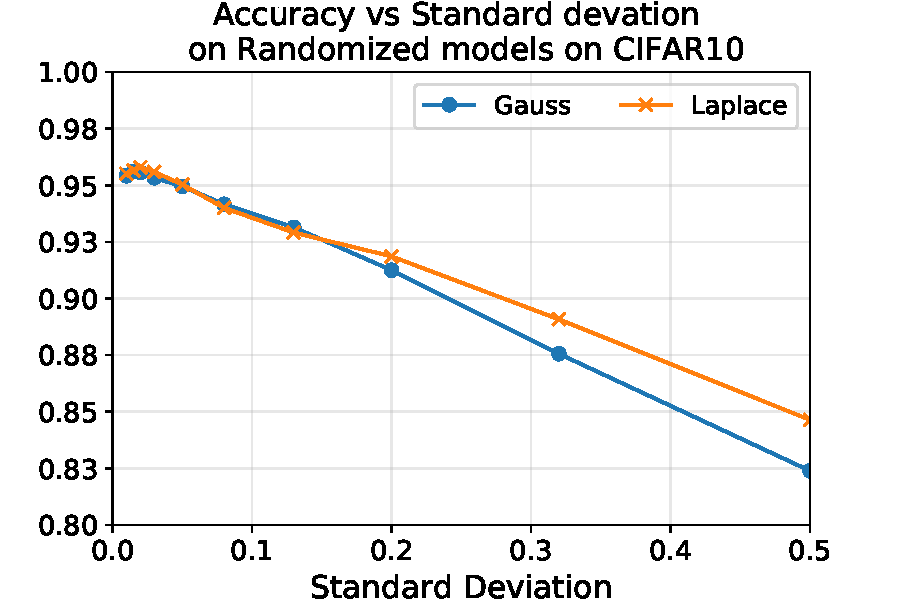
\includegraphics[scale=0.32]{figures/appendix3/acc_sd_CIFAR10.pdf}
      \caption{}
      \label{figure:ap3-acc_sd_CIFAR10}
  \end{subfigure}
  \begin{subfigure}[t]{0.31\textwidth}
      \centering
      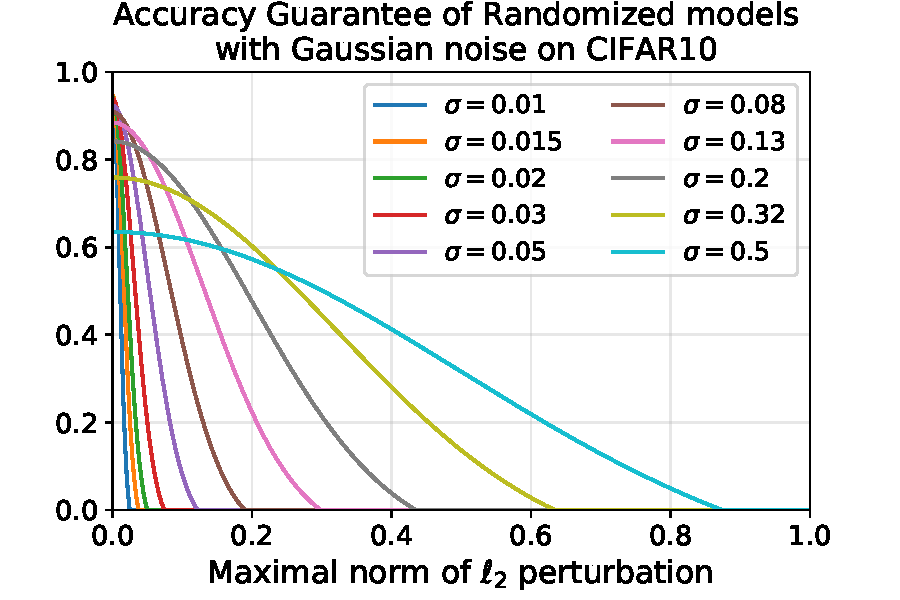
\includegraphics[scale=0.32]{figures/appendix3/gauss_certif_CIFAR10.pdf}
      \caption{}
      \label{figure:ap3-gauss_certif_CIFAR10}
  \end{subfigure}
  \begin{subfigure}[t]{0.31\textwidth}
      \centering
      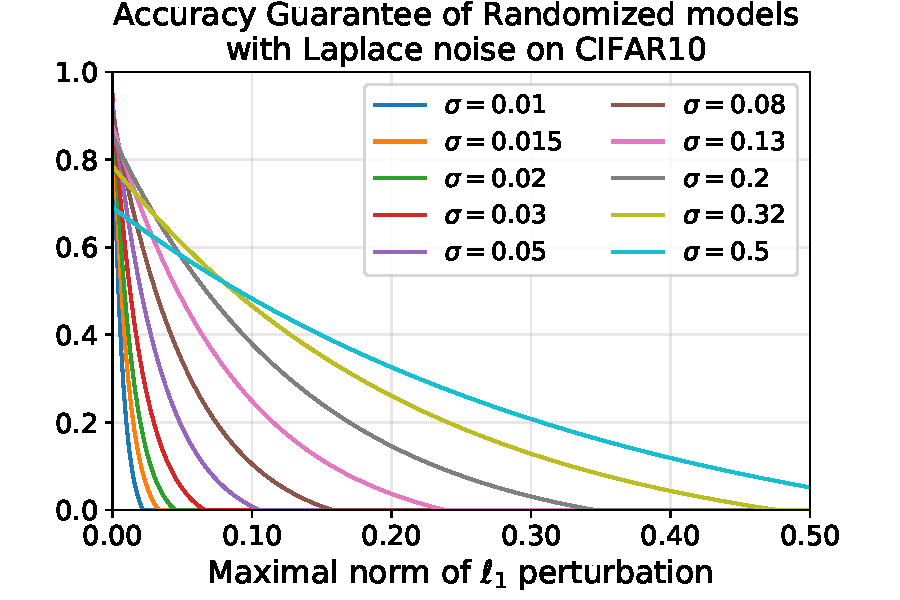
\includegraphics[scale=0.32]{figures/appendix3/laplace_certif_CIFAR10.pdf}
      \caption{}
      \label{figure:ap3-laplace_certif_CIFAR10}
  \end{subfigure}
  \caption{(a) Impact of the standard deviation of the injected noise on accuracy in a randomized model on CIFAR-10 dataset with a Wide ResNet architecture. (b) and (c) illustration of the guaranteed accuracy of different randomized models with Gaussian (b) and Laplace (c) noises given the norm of the adversarial perturbation.}
  \label{figure:ap3-cifar10_results}
\end{figure}

When injecting noise as a defense mechanism, regardless of the distribution it is drawn from, we observe (as in Figure~\ref{figure:ap3-acc_sd_CIFAR10}) that the accuracy decreases when the noise intensity grows.
In that sense, noise needs to be calibrated to preserve both accuracy and robustness against adversarial attacks, \ie, it needs to be large enough to preserve robustness and small enough to preserve accuracy.
Figure~\ref{figure:ap3-acc_sd_CIFAR10} shows the loss of accuracy on CIFAR10 from $0.95$ to $0.82$ (respectively $0.95$ to $0.84$) with noise drawn from a Gaussian distribution (respectively Laplace) with a standard deviation from $0.01$ to $0.5$.
Figure~\ref{figure:ap3-gauss_certif_CIFAR10} and \ref{figure:ap3-laplace_certif_CIFAR10} illustrate the theoretical lower bound on accuracy under attack of Theorem~\ref{theorem:ap3-bound} for different distributions and standard deviations.
The term in entropy of Theorem~\ref{theorem:ap3-bound} has been estimated using a Monte Carlo method with $10^4$ simulations.
The trade-off between accuracy and robustness from Theorem~\ref{theorem:ap3-bound} thus appears \wrt the noise intensity.
With small noises, the accuracy is high, but the guaranteed accuracy drops fast \wrt the magnitude of the adversarial perturbation.
Conversely, with bigger noises, the accuracy is lower but decreases slowly \wrt the magnitude of the adversarial perturbation.
These Figures also show that Theorem~\ref{theorem:ap3-bound} gives strong accuracy guarantees against small adversarial perturbations.
Next paragraph shows that in practice, randomized networks achieve much higher accuracy under attack than the theoretical bound, and keep this accuracy against much larger perturbations.


\paragraph{Performance of randomized networks under attacks and comparison to state of the art (Q2.2):}
\label{sec:perf_under_attack}

While Figure~\ref{figure:ap3-gauss_certif_CIFAR10} and \ref{figure:ap3-laplace_certif_CIFAR10} illustrated a theoretical robustness against growing adversarial perturbations, Table~\ref{table:ap3-accuracy_under_attack} illustrates this trade-off experimentally.
It compares the accuracy obtained under attack by a deterministic network with the one obtained by randomized networks with Gaussian and Laplace noises both with low ($0.01$) and high ($0.5$) standard deviations.
Randomized networks with a small noise lead to no loss in accuracy with a small robustness while high noise leads to a higher robustness at the expense of loss of accuracy ($\sim11$ points). 

\begin{table}[t]
  \centering
  \caption{Accuracy under attack on the CIFAR-10 dataset with a randomized Wide ResNet architecture. We compare the accuracy on natural images and under attack with different noise over 3 iterative attacks (the number of steps is next to the name) made with 80 Monte Carlo simulations to compute EoT attacks. The first line is the baseline, no noise has been injected.}
    \begin{tabular}{lccccc}
    \toprule
    \textbf{Distribution} & \textbf{Sd} & \textbf{Natural} & \textbf{$\ell_1$ -- EAD 60} & \textbf{$\ell_2$ -- C\&W 60} & \textbf{$\ell_\infty$ -- PGD 20} \\
    \midrule
    - & - & 0.958 & 0.035 & 0.034 & 0.384 \\
    \midrule
    \multirow{2}[0]{*}{Normal} & 0.01 & 0.954 & 0.193 & 0.294 & 0.408 \\
          & 0.50 & 0.824 & 0.448 & 0.523 & 0.587 \\
    \midrule
    \multirow{2}[0]{*}{Laplace} & 0.01 & 0.955 & 0.208 & 0.313 & 0.389 \\
          & 0.50 & 0.846 & 0.464 & 0.494 & 0.589 \\
    \bottomrule
    \end{tabular}%
  \label{table:ap3-accuracy_under_attack}%
\end{table}%

\begin{table}[t]
  \caption{Accuracy under attack of randomized neural network with different distributions and standard deviations versus adversarial training by~\citet{madry2018towards}. The PGD attack has been made with 20 step, an epsilon of 0.06 and a step size of 0.006 (input space between $-1$ and $+1$). The Carlini\&Wagner attack uses 30 steps, 9 binary search steps and a 0.01 learning rate. The first line refers to the baseline without attack.}
  \label{Results}
  \centering
  \begin{tabular}{ccccccc}
    \toprule
      & & \multirow{2}[0]{*}{\citet{madry2018towards}} & \multirow{2}[0]{*}{\textbf{Normal 0.32}} & \multirow{2}[0]{*}{\textbf{Laplace 0.32}} & \multirow{2}[0]{*}{\textbf{Normal 0.5}} & \multirow{2}[0]{*}{\textbf{Laplace 0.5}} \\
     \textbf{Attack} & \textbf{Steps} & & & \\
    \midrule
    -  & - & 0.873 & 0.876 & 0.891 & 0.824 & 0.846 \\ 
    $\ell_\infty$ -- PGD & 20 & 0.456 & 0.566 & 0.576 & 0.587 & 0.589 \\
    $\ell_2$ -- C\&W & 30 & 0.468 & 0.512 & 0.502 & 0.489 & 0.479 \\
    \bottomrule
  \end{tabular}
  \label{table:madry_vs_random}
\end{table}

Finally, Table~\ref{table:madry_vs_random} compares the accuracy and the accuracy under attack of randomized networks with Gaussian and Laplace distributions for different standard deviations against adversarial training from ~\citet{madry2018towards}.
We observe that the accuracy on natural images of both noise injection methods are similar to the one from~\cite{madry2018towards}.
Moreover, both methods are more robust than adversarial training to PGD and C\&W attacks.
As with all the experiments, to construct an EoT attack,  we use 80 Monte Carlo simulations at every step of PGD and C\&W attacks.
These experiments show that randomized defenses can be competitive given the intensity of noise injected in the network.
Note that these experiments have been led with $\EoT$ of size 80.
For much bigger sizes of $\EoT$ these results would be mitigated.
Nevertheless, the accuracy would never drop under the bounds illustrated in Figure~\ref{figure:ap3-cifar10_results}, since Theorem~\ref{theorem:ap3-bound} gives a bound that on the worst case attack strategy (including $\EoT$).

%%%%%%%%%%%%%%%%%%%%%%%%%%%%%%%%%%%%%%%%%%%%%%%%%%%%%%%%%%%%%%%%%%%%%%%%%%%%%%%
\section{Conclusion and future works}
\label{section:ap3-conclusion}
%%%%%%%%%%%%%%%%%%%%%%%%%%%%%%%%%%%%%%%%%%%%%%%%%%%%%%%%%%%%%%%%%%%%%%%%%%%%%%%

This paper brings new contributions to the field of provable defenses to adversarial attacks. Principled answers have been provided to key questions on the interest of randomization techniques, and on their loss of accuracy under attack. The obtained bounds have been illustrated in practice by conducting thorough experiments on baseline datasets such as CIFAR and ImageNet. We show in particular that a simple method based on injecting noise drawn from the Exponential family is competitive compared to baseline approaches while leading to provable guarantees. Future work will focus on investigating other noise distributions belonging or not to the Exponential family, combining randomization with more sophisticated defenses and on devising new tight bounds on the adversarial generalization gap.


\begin{Large}
MAT SUP
\end{Large}

%%%%%%%%%%%%%%%%%%%%%%%%%%%%%%%%%%%%%%%%%%%%%%%%%%%%%%%%%%%%%%%%%%%%%%%%%%%%%%%
\section{Notations and definitions}
%%%%%%%%%%%%%%%%%%%%%%%%%%%%%%%%%%%%%%%%%%%%%%%%%%%%%%%%%%%%%%%%%%%%%%%%%%%%%%%

Let us consider an output space $\mathcal{Y}$, and $\mathcal{F}_{\mathcal{Y}}$ a $\sigma$-$ algebra$ over $\mathcal{Y}$. We denote $\mathcal{P}(\mathcal{Y})$ the set of probability measures over $(\mathcal{Y},\mathcal{F}_{\mathcal{Y}})$.
Let $(\mathcal{Y'},\mathcal{F}_{\mathcal{Y'}})$ be a second measurable space, and $\phi$ a measurable mapping from $(\mathcal{Y},\mathcal{F}_{\mathcal{Y}})$ to $(\mathcal{Y'},\mathcal{F}_{\mathcal{Y'}})$. Finally Let us consider $\mu,\nu$ two measures on $(\mathcal{Y},\mathcal{F}_{\mathcal{Y}})$.

\textbf{Dominated measure:} $\mu$ is said to be dominated by $\nu$ (denoted $\mu \ll \nu$) if for all $Y \in \mathcal{F}_{\mathcal{Y}}$, $\ \nu(Y) = 0 \implies \mu(Y)=0$. If $\mu$ is dominated by $\nu$, there is a measurable function $h : \mathcal{Y} \rightarrow [0,+\infty)$ such that for all $Y \in \mathcal{F}_{\mathcal{Y}}$, $ \mu(Y)=\int_{Y} h \ d\nu$. $ h $ is called the Radon-Nikodym derivative of $\mu$ \wrt $\nu$ and is denoted $\frac{d \mu}{d \nu}$.
   
\textbf{Push-forward measure:} the push-forward measure of $\nu$ by $\phi$ (denoted $\phi \# \nu$) is the measure on $(\mathcal{Y'},\mathcal{F}_{\mathcal{Y'}})$ such that $\forall Z \in \mathcal{F}_{\mathcal{Y'}}, \ \phi \# \nu(Z) = \nu(\phi^{-1}(Z)) $.

\textbf{Convolution product:} the convolution of $\nu$ with $\mu$, denoted $\nu * \mu$ is the push-forward measure of $\nu \otimes \mu$ by the addition on $\mathcal{Y}$. Since the convolution between functions is defined accordingly, we use $*$ indifferently for measures and simple functions. 

\textbf{Modulus of continuity:} Let us consider $f:(E,\norm{\ \cdot\ }_E)\rightarrow(F,\norm{\ \cdot\ }_F)$. $f$ admits a non-decreasing modulus of continuity regarding $\norm{\ \cdot\ }_E$ and $\norm{\ \cdot\ }_F$ if there exists a non-decreasing function $\omega^{E,F}_f:\mathbb{R^+}\rightarrow\mathbb{R^+}$ such as for all $x,y\in E$, $\norm{f(y) - f(x)}_F \leq \omega^{E,F}_f(\norm{x - y}_E)$.


%%%%%%%%%%%%%%%%%%%%%%%%%%%%%%%%%%%%%%%%%%%%%%%%%%%%%%%%%%%%%%%%%%%%%%%%%%%%%%%
\section{Main proofs}
%%%%%%%%%%%%%%%%%%%%%%%%%%%%%%%%%%%%%%%%%%%%%%%%%%%%%%%%%%%%%%%%%%%%%%%%%%%%%%%

As a trade-off between completeness and conciseness, we delayed the proofs of our theorems to this section.

%%%%%%%%%%%%%%%%%%%%%%%%%%%%%%%%%%%%%%%%%%%%%%%%%%%%%%%%%%%%%%%%%%%%%%%%%%%%%%%
\subsection{Proof of Lemma~\ref{th::PropimpliesRobustness-appendix}}
%%%%%%%%%%%%%%%%%%%%%%%%%%%%%%%%%%%%%%%%%%%%%%%%%%%%%%%%%%%%%%%%%%%%%%%%%%%%%%%

\begin{lemma}
\label{th::PropimpliesRobustness-appendix}Let $\probmap$ be a probabilistic mapping, and
let  $d_{1}$ and $d_{2}$ be two metrics on $\mathcal{P}(\mathcal{Y})$.
If there exists a non decreasing function $ \phi: \mathbb{R} \to \mathbb{R}$ such that  $\forall \mu_1,\mu_2 \in \mathcal{P}(\mathcal{Y})$, $d_{1}(\mu_1,\mu_2) \leq \phi(d_{2}(\mu_1,\mu_2)) $, then the following holds: 
$$\probmap \text{ is } d_{2}\text{-}(\alpha, \epsilon, \gamma)\text{-robust} \implies \probmap \text{ is }d_{1}\text{-}(\alpha, \phi(\epsilon), \gamma)\text{-robust}$$
\end{lemma}

\begin{proof}
Let us consider a probabilistic mapping $\probmap$, $x \sim \mathcal{D}$, and $\tau \in B(\alpha)$, one has $d_{1}(\probmap(x),\probmap(x +\tau)) \leq \phi(d_{2}(\probmap(x),\probmap(x +\tau))) \leq \phi(\epsilon).$ Hence  $\mathbb{P}_{x\sim\mathcal{D}}\left[ \forall \tau \in B(\alpha),\ d_1(\probmap(x+\tau),\probmap(x)) \leq \phi(\epsilon) \right] \leq 1-\gamma$. By inverting the inequality, one gets the expected result.
\end{proof}

%%%%%%%%%%%%%%%%%%%%%%%%%%%%%%%%%%%%%%%%%%%%%%%%%%%%%%%%%%%%%%%%%%%%%%%%%%%%%%%
\subsection{Proof of Proposition~\ref{propsition:ap3-RobustTV-appendix}}
%%%%%%%%%%%%%%%%%%%%%%%%%%%%%%%%%%%%%%%%%%%%%%%%%%%%%%%%%%%%%%%%%%%%%%%%%%%%%%%


\begin{proposition}[Renyi-robustness implies TV-robustness]
\label{propsition:ap3-RobustTV-appendix}
Let $\probmap$ be a probabilistic mapping, then for all $\lambda\geq1$:
$$\probmap \text{ is }  d_{R,\lambda}\text{-}(\alpha, \epsilon, \gamma)\text{-robust} \implies \probmap \text{ is } d_{TV}\text{-}(\alpha, \epsilon', \gamma)\text{-robust}$$
$$\textnormal{ with } \epsilon' = \min \left(\frac{3}{2}\left(\sqrt{1 + \frac{4\epsilon}{9}} - 1\right)^{1/2}, \frac{\exp(\epsilon +1) -1}{\exp(\epsilon +1) +1}\right).$$


\end{proposition}


\begin{proof}
Given two probability measures $\mu_1$ and $\mu_2$ on $(\mathcal{Y},\mathcal{F}_{\mathcal{Y}})$, and $\lambda >0$ one wants to find a bound on $d_{TV}(\mu_1,\mu_2)$ as a functional of $d_{R,\lambda}(\mu_1,\mu_2)$. 

Thanks to~\cite{5605338}, one has $$ d_{KL}(\mu_1,\mu_2) \geq 2d_{TV}(\mu_1,\mu_2)^{2}+ \frac{4d_{TV}(\mu_1,\mu_2)^{4}}{9}. $$ From which it follows that $$d_{TV}(\mu_1,\mu_2)^{2} \leq \frac{9}{4}\left(\sqrt{1 + \frac{4d_{KL}(\mu_1,\mu_2)}{9}} - 1\right)$$
One thus finally gets: 
$$d_{TV}(\mu_1,\mu_2) \leq \frac{3}{2}\left(\sqrt{1 + \frac{4d_{KL}(\mu_1,\mu_2)}{9}} - 1\right)^{1/2}$$
Moreover, using inequality from~\cite{Vajda1970}, one gets:
$$d_{KL}(\mu_1,\mu_2) \geq \log\left(\frac{1 + d_{TV}(\mu_1,\mu_2)}{1 - d_{TV}(\mu_1,\mu_2)} \right) - \frac{2d_{TV}(\mu_1,\mu_2)}{1 + d_{TV}(\mu_1,\mu_2)}$$
For the sake of simplicity, since the second part of the right hand side of the equation is non increasing given $d_{TV}(\mu_1,\mu_2)$, and since $0\leq d_{TV}(\mu_1,\mu_2)\leq 1$  one gets:
$$d_{KL}(\mu_1,\mu_2) +1 \geq \log\left(\frac{1 + d_{TV}(\mu_1,\mu_2)}{1 - d_{TV}(\mu_1,\mu_2)} \right) $$
Hence, one gets:
$$ \frac{\exp(d_{KL}(\mu_1,\mu_2) +1) -1}{\exp(d_{KL}(\mu_1,\mu_2) +1) +1} \geq  d_{TV}(\mu_1,\mu_2) $$
By combining the two results, one obtains: $$ d_{TV}(\mu_1,\mu_2) \leq \min \left(\frac{3}{2}\left(\sqrt{1 + \frac{4 d_{KL}(\mu_1,\mu_2)}{9}} - 1\right)^{1/2}, \frac{\exp(d_{KL}(\mu_1,\mu_2) +1) -1}{\exp(d_{KL}(\mu_1,\mu_2) +1) +1} \right).$$
To conclude for $\lambda>1$ it suffices to use Lemma~\ref{th::PropimpliesRobustness-appendix}, and the monotony of Renyi divergence regarding $\lambda$.
\end{proof}

%%%%%%%%%%%%%%%%%%%%%%%%%%%%%%%%%%%%%%%%%%%%%%%%%%%%%%%%%%%%%%%%%%%%%%%%%%%%%%%
\subsection{Proof of Proposition~\ref{propsition:ap3-:postprocessing-appendix}}
%%%%%%%%%%%%%%%%%%%%%%%%%%%%%%%%%%%%%%%%%%%%%%%%%%%%%%%%%%%%%%%%%%%%%%%%%%%%%%%


\begin{proposition}[Data processing inequality]
\label{propsition:ap3-:postprocessing-appendix} 
Let us consider a probabilistic mapping $\probmap:\mathcal{X}\rightarrow\mathcal{P}(\mathcal{Y})$. Let us also denote $\rho:\mathcal{Y}\rightarrow\mathcal{Y}'$ a deterministic function.
If $U\sim \probmap(x)$ then the probability measure $M'(x)$ s.t. $\rho(U) \sim M'(x)$ defines a probabilistic mapping $M':\mathcal{X}\rightarrow\mathcal{P}(\mathcal{Y}')$.

For any $\lambda>1$ if $\probmap$ is $d_{R,\lambda}$-$(\alpha,\epsilon,\gamma)$ robust then $M'$ is also is $d_{R,\lambda}$-$(\alpha,\epsilon,\gamma)$ robust.
\end{proposition}

\begin{proof}
  Let us consider $\probmap$ a $d_{R,\lambda}$-$(\alpha,\epsilon,\gamma)$ robust algorithm. Let us also take $x\in \mathcal{X}$, and $\tau \in B(\alpha)$.
  Without loss of generality, we consider that $\probmap(x)$, and $\probmap(x+\tau)$ are dominated by the same measure $\mu$.
  Finally let us take $\rho$ a measurable mapping from $(\mathcal{Y},\mathcal{F}_{\mathcal{Y}})$ to $(\mathcal{Y'},\mathcal{F}_{\mathcal{Y'}})$. For the sake of readability we denote $\probmap(x) =\nu_1$ and $M(x +\tau)=\nu_2$ (therefore $M'(x)=\rho \#\nu_1$, and $M'(x +\tau)=\rho \#\nu_2$).

  Since $\mu >> \nu_1, \nu_2$, one has $\rho \# \mu >> \rho \# \nu_1, \rho \#\nu_2$. Hence one has 
  \begin{align}
      d_{R,\lambda}(\rho \# \nu_1,\rho \# \nu_2) &= \frac{1}{\lambda - 1} \log \int_{\mathcal{Y}} \left(\frac{d\rho \# \nu_1}{d \rho \# \mu}\right)^{\lambda} \left(\frac{d\rho \# \nu_2}{d \rho \# \mu}\right)^{1-\lambda} d\rho \# \mu = \frac{1}{\lambda - 1} \log \int_{\mathcal{Y}} \left(\frac{d\rho \# \nu_1}{d \rho \# \nu_2}\right)^{\lambda} d\rho \# \nu_2\\
      \intertext{ Simply using the transfer theorem, one gets}
       d_{R,\lambda}(\rho \# \nu_1,\rho \# \nu_2) &= \frac{1}{\lambda - 1} \log \int_{\mathcal{Y'}} \left(\frac{d\rho \# \nu_1}{d \rho \# \nu_2} \circ \rho \right)^{\lambda} d\nu_2\\
      \intertext{Since $\left(\frac{d\rho \# \nu_1}{d \rho \# \nu_2} \circ \rho \right)= \mathbb{E}\left(\frac{d\nu_{1}}
     {d\nu_{2}}\big |\rho^{-1}(\mathcal{F}_{\mathcal{Y}})\right)$ one easily gets the following:}
     d_{R,\lambda}(\rho \# \nu_1,\rho \# \nu_2) & = \frac{1}{\lambda - 1} \log \int_{\mathcal{Y'}} \left(\frac{d\rho \# \nu_1}{d \rho \# \nu_2} \circ \rho \right)^{\lambda} d\nu_2 =  \frac{1}{\lambda - 1} \log \int_{\mathcal{Y'}} \mathbb{E}\left(\frac{d\nu_{1}}
     {d\nu_{2}}\big |\rho^{-1}(\mathcal{F}_{\mathcal{Y}})\right)^{\lambda} d\nu_{2}\\
     \intertext{Finally, by using the Jensen inequality, and the property of the conditional expectation, one has}
     d_{R,\lambda}(\rho \# \nu_1,\rho \# \nu_2)& \leq \frac{1}{\lambda - 1} \log \int_{\mathcal{Y'}} \mathbb{E}\left(\frac{d\nu_{1}}
     {d\nu_{2}}^{\lambda}\big |\rho^{-1}(\mathcal{F}_{\mathcal{Y}})\right) d\nu_{2}= \frac{1}{\lambda - 1} \log \int_{\mathcal{Y'}} \frac{d\nu_{1}}
     {d\nu_{2}}^{\lambda} d\nu_{2} = d_{R,\lambda}(\nu_{1},\nu_{2}).
  \end{align}
\end{proof}

%%%%%%%%%%%%%%%%%%%%%%%%%%%%%%%%%%%%%%%%%%%%%%%%%%%%%%%%%%%%%%%%%%%%%%%%%%%%%%%
\subsection{Proof of Theorem~\ref{theorem:ap3-netrob-appendix}}
%%%%%%%%%%%%%%%%%%%%%%%%%%%%%%%%%%%%%%%%%%%%%%%%%%%%%%%%%%%%%%%%%%%%%%%%%%%%%%%

\begin{lemma}
\label{theorem:ap3-exprob-appendix}

Let $\psi:\ \mathcal{X} \rightarrow \mathbb{R}^{n}$ be a mapping. For any $\alpha\geq0$ and for any norms $\norm{\ \cdot\ }_A$ and $\norm{\ \cdot\ }_B$, one can define $\Delta^{A,B}_{\alpha}(\psi) \triangleq \sup\limits_{ x,y \in \mathcal{X}, \norm{x - y}_A \leq \alpha} \norm{\psi(x) - \psi(y)}_B$. Let $X$ be a random variable. We denote $\probmap(x)$ the probability measure of the random variable $\psi(x)+X$. 
\begin{itemize}
    \item If $X\sim E_{F}(\theta,t,k)$  where $t$ and $k$ have non-decreasing modulus of continuity $\omega_t$ and $\omega_k$. 

Then for any $\alpha \geq 0$, $\probmap$ defines a probabilistic mapping that is $d_{R,\lambda}$-$(\alpha,\epsilon)$ robust
with $\epsilon = \norm{\theta}_2 \omega^{B,2}_t(\Delta^{A,B}_{\alpha}(\phi)) +\omega_k^{B,1}(\Delta^{A,B}_{\alpha}(\phi)) $ where $\norm{\ \cdot\ }_2$ is the norm corresponding to the scalar product in the definition of the exponential family density function and $\norm{\ \cdot\ }_1$ is here the absolute value on $\mathbb{R}$.
%Although the Gaussian distribution does not satisfy the modulus of continuity constraint on $t$, we still have robustness for Gaussian noise injection. Let
\item If $X$ is a centered Gaussian random variable with a non degenerated matrix parameter $\Sigma$. Then for any $\alpha \geq 0$, $\probmap$ defines a probabilistic mapping that is $d_{R,\lambda}$-$(\alpha,\epsilon)$ robust
with $ \epsilon = \frac{\lambda \Delta^{A,2}_{\alpha}(\phi)^2 }{2 \sigma_{min}(\Sigma) } $ where $\norm{\ \cdot\ }_2$ is the canonical Euclidean norm on $\mathbb{R}^n$.
\end{itemize}
\end{lemma}


\begin{proof}
  Let us consider $\probmap$ the probabilistic mapping constructed from noise injections respectively drawn from 1) an exponential family with non-decreasing modulus of continuity, or 2) a non degenerate Gaussian.
  Let us take $x \in \mathcal{X}$, and $\tau \in B(\alpha)$.
  Without loss of generality, we consider that $\probmap(x)$, and $\probmap(x + \tau)$ are dominated by the same measure $\mu$.
  Let us also denote, $p_F$ the Radon-Nikodym derivative of the noise drawn in 1) with respect to $\mu$, $p_G$ the Radon-Nikodym derivative of the noise drawn or in 2) with respect to $\mu$ and $ \delta_a$ the Dirac function mapping any element to $1$ if it equals $a$ and to 0 otherwise.

  1)\begin{align*}
    d_{R,\lambda} \left( \probmap(x), \probmap(x + \tau) \right) &= d_{R, \lambda} \left(\nu * \delta_{\psi(x)}, \nu * \delta_{\psi(x + \tau)}  \right) \\
    &\leq d_{R,\infty}\left(\nu * \delta_{\psi(x)},\nu * \delta_{\psi(x+\tau)}  \right) \\
    &=\log \sup\limits_{z \in \mathbb{R}^{n}} \frac{(p_F * \delta_{\psi(x)})(z)}{(p_F * \delta_{\psi(x+\tau)})(z)} \\
    &=\log \sup\limits_{z \in \mathbb{R}^{n}} \exp\left(<t(z-\psi(x)) - t(z-\psi(x + \tau)),\theta> \right. \\
    \quad &+ \left. k(z -\psi(x))-k(z-\psi(x +\tau)) \right) \\
    &\leq  \sup\limits_{z \in \mathbb{R}^{n}} \norm{\theta}_2 \norm{t(z-\psi(x)) - t(z-\psi(x + \tau))}_2 + | k(z-\psi(x)) - k(z-\psi(x + \tau)) | \\
    &\leq \norm{\theta}_2 \omega^{B,2}_t(\norm{\psi(x + \tau) - \psi(x)}_B) +\omega^{B,1}_k(\norm{\psi(x + \tau) - \psi(x)}_B) \\
    &\leq \norm{\theta}_2 \omega^{B,2}_t(\Delta^{A,B}_{\alpha}(\psi)) +\omega^{B,1}_k(\Delta^{A,B}_{\alpha}(\psi))
  \end{align*}

   2)\begin{align}
      & d_{R,\lambda}\left( \probmap(x),\probmap(x+\tau) \right) = \frac{1}{\lambda -1}\log \int_{\mathbb{R}^{n}} \left(p_G * \delta_{\psi(x)}\right)^{\lambda}\times \left(p_G* \delta_{\psi(x+\tau)}\right)^{1-\lambda} d\mu \\\\
      &= \frac{1}{\lambda -1}\log \int_{\mathbb{R}^{n}} \frac{\exp\left\{-1/2\left(\lambda\left(z - \psi(x)\right)^\top\Sigma^{-1}\left(z - \psi(x)\right) + (1-\lambda)\left(z - \psi(x+\tau)\right)^\top\Sigma^{-1}\left(z - \psi(x+\tau)\right)\right)\right\}}{(2 \pi)^{n/2}|\Sigma|^{1/2}}  dz \\
      &= \frac{-\left(\lambda \psi(x)^\top\Sigma^{-1}\psi(x) + (1-\lambda) \psi(x+\tau)^\top\Sigma^{-1}\psi(x+\tau) - \left(\lambda \psi(x) + (1- \lambda) \psi(x+\tau)\right)^\top\Sigma^{-1}\left(\lambda \psi(x) + (1- \lambda) \psi(x+\tau)\right)\right)}{2\lambda -2} \\
      &= \frac{\lambda^{2} - \lambda}{2(\lambda -1)} (\psi(x) - \psi(x+\tau))^\top \Sigma^{-1}(\psi(x) - \psi(x+\tau))\\
      &\leq \frac{\lambda}{2} \sigma_{max}\left(\Sigma^{-1}\right) \norm{(\psi(x) - \psi(x+\tau))}_2^2 \leq \frac{\lambda \Delta^{A,2}_{\alpha}(\psi)^2 }{ 2 \sigma_{min}(\Sigma)}.
    \end{align}
\end{proof}


\begin{theorem}[Exponential family ensures robustness]
\label{theorem:ap3-netrob-appendix}
Let us denote $\mathcal{N}_{X}^i(\ \cdot\ )=\phi^n\circ \cdots \circ\phi^{i+1}(\mathcal{N}_{|i}(\ \cdot\ )+X)$ with $X$ a random variable. Let us also consider $\norm{\ \cdot\ }_{A}$, and $\norm{\ \cdot\ }_{B}$ two arbitrary norms respectively on $\mathcal{X}$ and on the output space of $\mathcal{N}_{X}^i$.




\begin{itemize}
  \item If $X\sim E_{F}(\theta,t,k)$  where $t$ and $k$ have non-decreasing modulus of continuity $\omega_t$ and $\omega_k$. Then for any $\alpha \geq 0$, $\mathcal{N}_{X}^i(\ \cdot\ )$ defines a probabilistic mapping that is $d_{R,\lambda}$-$(\alpha,\epsilon)$ robust with $\epsilon = \norm{\theta}_2 \omega^{B,2}_t(\Delta^{A,B}_{\alpha}(\phi)) +\omega_k^{B,1}(\Delta^{A,B}_{\alpha}(\phi)) $ where $\norm{\ \cdot\ }_2$ is the norm corresponding to the scalar product in the definition of the exponential family density function and $\norm{\ \cdot\ }_1$ is here the absolute value on $\mathbb{R}$. The notion of continuity modulus is defined in the preamble of this supplementary material.
    
%Although the Gaussian distribution does not satisfy the modulus of continuity constraint on $t$, we still have robustness for Gaussian noise injection. Let
\item If $X$ is a centered Gaussian\footnote{Although the Gaussian distribution belongs to the exponential family, it does not satisfy the modulus of continuity constraint on $t$ and its robustness has to be proved differently.} random variable with a non degenerated matrix parameter $\Sigma$. Then for any $\alpha \geq 0$, $\mathcal{N}_{X}^i(\ \cdot\ )$ defines a probabilistic mapping that is $d_{R,\lambda}$-$(\alpha,\epsilon)$ robust
with $ \epsilon = \frac{\lambda \Delta^{A,2}_{\alpha}(\phi)^2 }{2 \sigma_{min}(\Sigma) } $ where $\norm{\ \cdot\ }_2$ is the canonical Euclidean norm on $\mathbb{R}^n$.
\end{itemize}
\end{theorem}



\begin{proof}
This theorem is a direct consequence of Lemma~\ref{theorem:ap3-exprob-appendix} and Proposition~\ref{propsition:ap3-:postprocessing-appendix}. By applying Lemma~\ref{theorem:ap3-exprob-appendix} to $\psi=\mathcal{N}_{|i}$ and Proposition~\ref{propsition:ap3-:postprocessing-appendix} to $\rho=\phi^n\circ \cdots \circ\phi^{i+1}$, we immediately get the result.
\end{proof}

%%%%%%%%%%%%%%%%%%%%%%%%%%%%%%%%%%%%%%%%%%%%%%%%%%%%%%%%%%%%%%%%%%%%%%%%%%%%%%%
\subsection{Proof of Theorem~\ref{theorem:ap3-bound-appendix}}
%%%%%%%%%%%%%%%%%%%%%%%%%%%%%%%%%%%%%%%%%%%%%%%%%%%%%%%%%%%%%%%%%%%%%%%%%%%%%%%


\begin{theorem}[Adversarial generalization gap bound in the randomized setting]

\label{theorem:ap3-bound-appendix}
Let $\probmap$ be the probabilistic mapping at hand. Let suppose that  $\probmap$ is $d_{R,\lambda}$-$(\alpha,\epsilon)$ robust for some $\lambda\geq1$ then:

$$|\advRisk(\probmap)-\Risk(\probmap)|\leq 1-e^{-\epsilon}\mathbb{E}_x\left[e^{-H(\probmap(x))}\right]$$
where $H$ is the Shannon entropy: $H(p)=-\sum_i p_i \log(p_i)$
\end{theorem}

\begin{proof}
Let $\probmap$ be a randomized network with a noise $X$ injected at layer $i$. We have:
\begin{align*}
  \left|\advRisk(\probmap)-\Risk(\probmap)\right|  &= \left|\mathbb{E}_{(x,y)}\left[ \sup_{\tau/\norm{\tau}\leq\alpha} \mathbb{E}_{y'\sim \probmap(x+\tau)}\left[ \mathds{1}\left( y_1\neq y\right) \right]-  \mathbb{E}_{y_2\sim \probmap(x)}\left[ \mathds{1}\left(y'\neq y\right)\right]\right]\right| \\
  &=\left|\mathbb{E}_{(x,y)}\left[ \sup_{\tau/\norm{\tau}\leq\alpha} \mathbb{E}_{y_1\sim \probmap(x+\tau),y_2\sim \probmap(x)}\left[ \mathds{1}\left(y_1\neq y\right)-  \mathds{1}\left(y_2\neq y\right) \right]\right]\right|\\
  &\leq\mathbb{E}_{(x,y)}\left[ \sup_{\tau/\norm{\tau}\leq\alpha} \mathbb{E}_{y_1\sim \probmap(x+\tau),y_2\sim \probmap(x)}\left[\left| \mathds{1}\left(y_1\neq y\right)-  \mathds{1}\left(y_2\neq y\right)\right|\right]\right]\\
  &\leq\mathbb{E}_{(x,y)}\left[ \sup_{\tau/\norm{\tau}\leq\alpha} \mathbb{E}_{y_1\sim \probmap(x+\tau),y_2\sim \probmap(x)}\left[ \mathds{1}\left(y_1\neq y_2\right)\right]\right]\\
  &=\mathbb{E}_{(x,y)}\left[\sup_{\tau/\norm{\tau}\leq\alpha}\mathbb{P}_{y_1\sim \probmap(x+\tau),y_2\sim \probmap(x)}(y_1\neq y_2)\right]
\end{align*}

For two discrete random independent variables of law $P=(p_1, \cdots ,p_K)$ and $Q=(q_1, \cdots ,q_K)$, thanks to Jensen's inequality: 
$$\mathbb{P}(P=Q)=\sum_{i=1}^K p_i q_i \geq \exp{(\sum_{i=1}^K p_i \log q_i)}=\exp{(-d_{KL}(P,Q)-H(P))}$$

Then we have:
\begin{align*}
  \mathbb{E}_{(x,y)}\left[\sup_{\tau/\norm{\tau}\leq\alpha}\mathbb{P}_{y_1\sim \probmap(x+\tau),y_2\sim \probmap(x)}(y_1\neq y_2)\right] &\leq\mathbb{E}_{(x,y)}\left[\sup_{\tau/\norm{\tau}\leq\alpha}1-e^{-d_{KL}(\probmap(x),\probmap(x+\tau))-H(\probmap(x))} \right] \\
  &\leq \mathbb{E}_{(x,y)}\left[1-e^{-\epsilon-H(\probmap(x))} \right] \\
  &= 1 - e^{-\epsilon}\mathbb{E}_x\left[e^{-H(\probmap(x))}\right] \\
\end{align*}

\end{proof}


%%%%%%%%%%%%%%%%%%%%%%%%%%%%%%%%%%%%%%%%%%%%%%%%%%%%%%%%%%%%%%%%%%%%%%%%%%%%%%%
\section{Additional results and discussions}
%%%%%%%%%%%%%%%%%%%%%%%%%%%%%%%%%%%%%%%%%%%%%%%%%%%%%%%%%%%%%%%%%%%%%%%%%%%%%%%
In this section, we give some additional results on both the strength of the Renyi-divergence and a bound on the generalization gap for TV-distance.

%%%%%%%%%%%%%%%%%%%%%%%%%%%%%%%%%%%%%%%%%%%%%%%%%%%%%%%%%%%%%%%%%%%%%%%%%%%%%%%
\subsection{About Renyi divergence}
%%%%%%%%%%%%%%%%%%%%%%%%%%%%%%%%%%%%%%%%%%%%%%%%%%%%%%%%%%%%%%%%%%%%%%%%%%%%%%%

In the main submission, we chose to use the Renyi-robustness as the principled measure of robustness. Since Renyi-divergence is a good surrogate for the trivial distance (which is a generalization of the $0-1$-loss for probabilistic mappings), we supported this statement by showing that Renyi-divergence is stronger than TV-distance.
In this section, we extend this result to most of the classical divergences used in Machine Learning and show that Renyi-divergence is stronger than all of them.   

Let us consider an output space $\mathcal{Y}$, $\mathcal{F}_{\mathcal{Y}}$ a $\sigma$-$ algebra$ over $\mathcal{Y}$, and $\mu_1,\mu_2,\nu$ three measures on $(\mathcal{Y},\mathcal{F}_{\mathcal{Y}})$, with $\mu_1,\mu_2$ in the set of probability measures over $(\mathcal{Y},\mathcal{F}_{\mathcal{Y}})$ denoted $\mathcal{P}(\mathcal{Y})$.
One has $\nu >> \mu_1,\mu_2$ and one denotes $g_1$ and $g_2$ the Radon-Nikodym derivatives with respect to $\nu$.

\textbf{The Separation distance:}
$$d_{S}(\mu_1,\mu_2) \triangleq \underset{\{z\} \in \mathcal{F}_{\mathcal{Y}}}{\sup}  1 - \frac{\mu_1(\{z\})}{\mu_2(\{z\})}. $$


\textbf{The Hellinger distance:} 
$$ d_{H}(\mu_1,\mu_2) \triangleq  \left[ \int_{\mathcal{Y}} \left(\sqrt{g_1} - \sqrt{g_2} \right)^{2} d \nu \right]^{1/2}.$$


\textbf{The Prokhorov metric:} 
$$d_{P}(\mu_1,\mu_2) \triangleq \inf\left\{ \zeta >0: \mu_1(B) \leq \mu_2(B^{\zeta}) + \zeta \textnormal{ for all Borel sets } B\right\}
\textnormal{ where } B^{\zeta} = \{x : \inf\limits_{y \in B} d_{\mathcal{Y'}}(x,y)\leq \zeta \}.$$


\textbf{The Discrepancy metric:}
$$d_{D}(\mu_1,\mu_2) \triangleq \underset{\textnormal{all closed balls B}}{\sup} \left| \mu_1(B) - \mu_2(B) \right|.$$

\begin{lemma}\label{lemma:separation-appendix}
Given two probability measures $\mu_1$ and $\mu_2$ on $(\mathcal{Y},\mathcal{F}_{\mathcal{Y}})$  the Separation metric and the Renyi divergence satisfy the following relation: $d_S(\mu_1,\mu_2) \leq d_{R,\infty}(\mu_1,\mu_2)$
\end{lemma}

\begin{proof}
The function $x: \to 1-x - \left|\ln(x)\right|$ is negative on $\mathbb{R}$, therefore for any $\{z\} \in \mathcal{Y}$ one has $1-\frac{\mu_1(\{z\})}{\mu_2(\{z\})} \leq \left|\ln\frac{\mu_1(\{z\})}{\mu_2(\{z\})}\right|$, hence $\sup_{\{z\} \in \mathcal{F}_{\mathcal{Y}}} 1-\frac{\mu_1(\{z\})}{\mu_2(\{z\})} \leq \sup_{\{z\} \in \mathcal{F}_{\mathcal{Y}}}\left|\ln\frac{\mu_1(\{z\})}{\mu_2(\{z\})}\right| \leq \sup_{Z \in \mathcal{F}_{\mathcal{Y}}}\left|\ln\frac{\mu_1(Z)}{\mu_2(Z)}\right| = d_{R,\infty}(\mu_1,\mu_2)$
\end{proof}

\begin{theorem}
Let $\probmap$ be the probabilistic mapping, then for all $\lambda >1$ if $\probmap \text{ is }  d_{R,\lambda}\text{-}(\alpha, \epsilon, \gamma)\text{-robust}$ 
the following assertions holds:
\begin{itemize}
\item[(1)] $\probmap$ is $d_{H}\text{-}(\alpha, \sqrt{\epsilon}, \gamma)\text{-robust}.$
\item[(2)] $\probmap$ is $d_{P}\text{-}(\alpha, \epsilon', \gamma)\text{-robust} \textbf{ and } d_{D}\text{-}(\alpha, \epsilon', \gamma)\text{-robust}$, for $\epsilon' = \min \left(\frac{3}{2}\left(\sqrt{1 + \frac{4\epsilon}{9}} - 1\right)^{1/2}, \frac{\exp(\epsilon +1) -1}{\exp(\epsilon +1) +1}\right).$
\item[(3)] $\probmap \text{ is } d_{W}\text{-}(\alpha, \epsilon', \gamma)\text{-robust} \text{ with }\epsilon' = \min \left(\frac{3}{2 diam(\mathcal{Y})}\left(\sqrt{1 + \frac{4\epsilon}{9}} - 1\right)^{1/2}, \frac{\exp(\epsilon +1) -1}{ diam(\mathcal{Y}) (\exp(\epsilon +1) +1)}\right)$.
\item[(4)] if $\lambda =\infty$, $ \probmap \text{ is } d_{S}\text{-}(\alpha, \epsilon, \gamma)\text{-robust}.$
\end{itemize}
\end{theorem}


\begin{proof}
\begin{itemize}
\item[ ]
\item[(1)] The proof is a simple adaptation of Proposition~\ref{propsition:ap3-RobustTV-appendix} using the inequality $d_H(\mu_1,\mu_2)^{2} \leq d_{KL}(\mu_1,\mu_2)$~\cite{AGibbsMetrics2002} and Lemma~\ref{th::PropimpliesRobustness-appendix}.\\
\item[(2)] Using the inequalities  $d_D(\mu_1,\mu_2) \leq d_{TV}(\mu_1,\mu_2)$~\cite{AGibbsMetrics2002} and  $d_P(\mu_1,\mu_2) \leq d_{TV}(\mu_1,\mu_2)$~\cite{huber2011robust}, the proof is immediate, using Theorem~\ref{th::PropimpliesRobustness-appendix} and Lemma~\ref{th::PropimpliesRobustness-appendix}.
\item[(3)] The proof is adapted from Proposition~\ref{propsition:ap3-RobustTV-appendix} using the inequality $d_W(\mu_1,\mu_2) \leq diam(\mathcal{Y}) d_{TV}(\mu_1,\mu_2)$~\cite{AGibbsMetrics2002}.
\item[(4)]The result is a straightforward application of Lemma~\ref{lemma:separation-appendix}, and Lemma~\ref{th::PropimpliesRobustness-appendix}.
\end{itemize}
\end{proof}


%%%%%%%%%%%%%%%%%%%%%%%%%%%%%%%%%%%%%%%%%%%%%%%%%%%%%%%%%%%%%%%%%%%%%%%%%%%%%%%
\subsection{Generalization gap with TV-robustness}
%%%%%%%%%%%%%%%%%%%%%%%%%%%%%%%%%%%%%%%%%%%%%%%%%%%%%%%%%%%%%%%%%%%%%%%%%%%%%%%

In the main paper, we give a bound on the generalization gap based on the Renyi-robustness. We extend this result to the TV-robustness, highlighting the fact that generalization gap could be derived from any of the above divergences.

\begin{theorem}

\label{theorem:ap3-boundTV-appendix}
Let $\probmap$ be the probabilistic mapping at hand. Let us suppose that  $\probmap$ is $d_{TV}$-$(\alpha,\epsilon)$ robust then:
$$|\advRisk(\probmap)-\Risk(\probmap)|\leq 1-(\mathbb{E}_x\left[e^{-H_c(\probmap(x))}\right]-\epsilon)$$
where $H_c$ is the collision entropy: $H_c(p)=-\log(\sum_i p_i^2)$
\end{theorem}
\begin{proof}
For two discrete random independent variables of law $P=(p_1, \cdots ,p_K)$ and $Q=(q_1, \cdots ,q_K)$, thanks to Jensen's inequality: 
$$\mathbb{P}(P=Q)=\sum_{i=1}^K p_i q_i=\sum_{i=1}^K p_i^2-\sum p_i(p_i-q_i)\geq e^{-H_c(P)}-d_{TV}(P,Q)$$
because, for any $i \in [K]$, $p_i-q_i\leq d_{TV}(P,Q)$.

Then, the proof is a simple adaptation of the model of proof from Theorem~\ref{theorem:ap3-bound-appendix}.
\end{proof}


%%%%%%%%%%%%%%%%%%%%%%%%%%%%%%%%%%%%%%%%%%%%%%%%%%%%%%%%%%%%%%%%%%%%%%%%%%%%%%%
\section{Additional empirical evaluation}
%%%%%%%%%%%%%%%%%%%%%%%%%%%%%%%%%%%%%%%%%%%%%%%%%%%%%%%%%%%%%%%%%%%%%%%%%%%%%%%

Due to space limitations, we had to defer the thorough description of our experimental setup and the results of some additional experiments.

%%%%%%%%%%%%%%%%%%%%%%%%%%%%%%%%%%%%%%%%%%%%%%%%%%%%%%%%%%%%%%%%%%%%%%%%%%%%%%%
\subsection{Architectures \& Hyper-parameters}
%%%%%%%%%%%%%%%%%%%%%%%%%%%%%%%%%%%%%%%%%%%%%%%%%%%%%%%%%%%%%%%%%%%%%%%%%%%%%%%

We conduct experiments with 3 different dataset:
\begin{itemize}
    \item CIFAR-10 and CIFAR-100 datasets, which are composed of 50K training samples, $10000$ test samples and respectively 10 and 100 different classes. Images are trained and evaluated with a resolution of 32 by 32 pixels. 
    \item ImageNet dataset, which is composed of $\sim1.2$M training examples, $50K$ test samples and $1000$ classes. Images are trained and evaluated with a resolution of 299 by 299 pixels. 
\end{itemize}

For CIFAR-10 and CIFAR-100 \cite{krizhevsky2009learning}, we used a Wide ResNet architecture \cite{ZagoruykoK16} which is a variant of the ResNet model from \cite{He_2016_CVPR}.
We used 28 layers with a widen factor of 10.
We trained all the networks for 200 epochs, a batch size of 400, dropout 0.3 and Leaky Relu activation with a slope on $\mathbb{R}^-$ of 0.1. We used the cross entropy loss with Momentum 0.9 and  a piecewise constant learning rate of 0.1, 0.02, 0.004 and 0.00008 after respectively 7500, 15000 and 20000 steps.
The networks achieve for CIFAR10 and 100 a TOP-1 accuracy of 95.8\% and 79.1\% respectively on test images. 

For ImageNet \cite{imagenet_cvpr09}, we used an Inception ResNet v2 \cite{szegedy2017inception} which is the sate of the art architecture for this dataset and achieved a TOP-1 accuracy of 80\%.
For the training of ImageNet, we used the same hyper parameters setting as the original implementation.
We trained the network for 120 epochs with a batch size of 256, dropout 0.8, Relu as activation function.
All evaluations were done with a single crop on the non-blacklisted subset of the validation set.


%%%%%%%%%%%%%%%%%%%%%%%%%%%%%%%%%%%%%%%%%%%%%%%%%%%%%%%%%%%%%%%%%%%%%%%%%%%%%%%
\subsection{Evaluation under attack}
%%%%%%%%%%%%%%%%%%%%%%%%%%%%%%%%%%%%%%%%%%%%%%%%%%%%%%%%%%%%%%%%%%%%%%%%%%%%%%%

We evaluate our models against the strongest possible attacks from the literature using different norms ($\ell_1$, $\ell_2$ and $\ell_\infty$) which are all optimization based attacks.
On their guide to evaluate robustness, \citet{carlini2019evaluating} proposed the three following attacks for each norm: 

\paragraph{$\ell_2$ -- Carlini \& Wagner attack and $\ell_1$ -- ElasticNet attack}
The $\ell_2$ Carlini \& Wagner attack ($C\&W$) introduced by~\citet{carlini2017towards} is formulated as:
\begin{equation}
  \min_{x+r\in \mathcal{X} } c \times \norm{r}_2+g(x+r)
\end{equation}
where $g$ is a function such that $g(y)\geq 0$ iff $f(y)=l'$ with $l'$ the target class.
The authors listed some $g$ functions.
We choose the following one:
\begin{equation}
  g(x)=\max(F_{k(x)}(x)-\max_{i\neq k(x)}(F_i(x)),-\kappa)
\end{equation}
where $F$ is the softmax function and $\kappa$ a positive constant.

Instead of using box-constrained L-BFGS~\cite{Szegedy2013IntriguingPO} as in the original attack, the authors use instead a new variable for $x+r$:
\begin{equation}
  x+r=\frac{1}{2} (\tanh(w)+1)
\end{equation}
\medbreak
Then a binary search is performed to optimize the constant $c$ and ADAM or SGD for computing an optimal solution.

$\ell_1$ -- ElasticNet attack is an adaptation of $\ell_2$ C\&W attack where the objective is adaptive to $\ell_1$ perturbations:
\begin{equation}
  \min_{x+r\in \mathcal{X} } c_1\times\norm{r}_1+c_2\times\norm{r}_2+g(x+r)
\end{equation}


\paragraph{$\ell_\infty$ -- PGD attack.}
The PGD attack proposed by~\citet{madry2018towards} is a generalization of the iterative FGSM attack proposed by~\citet{kurakin2016adversarial}. The goal of the adversary is to solve the following problem:
$$\argmax_{\norm{r}_p \leq \epsilon} \mathcal{L}(F_{\theta}(x+r),y) $$
In practice, the authors proposed an iterative method to compute a solution:
$$x^{t+1}=P_{x \oplus r}(x^t+\alpha \sign (\nabla_x\mathcal{L}(F_\theta(x^t),y)))$$
Where $x \oplus r$ is the Minkowski sum between $\{x\}$ and $\{r \text{~s.t.~} \norm{r}_p \leq \epsilon\}$, $\alpha$ a gradient step size, $P_S$ is the projection operator on $S$ and $x^0$ is randomly chosen in $x \oplus r$. 

\subsection{Detailed results on CIFAR-10 and CIFAR-100}

\begin{figure}[htb]
  \centering
  \begin{subfigure}[t]{0.31\textwidth}
    \centering
    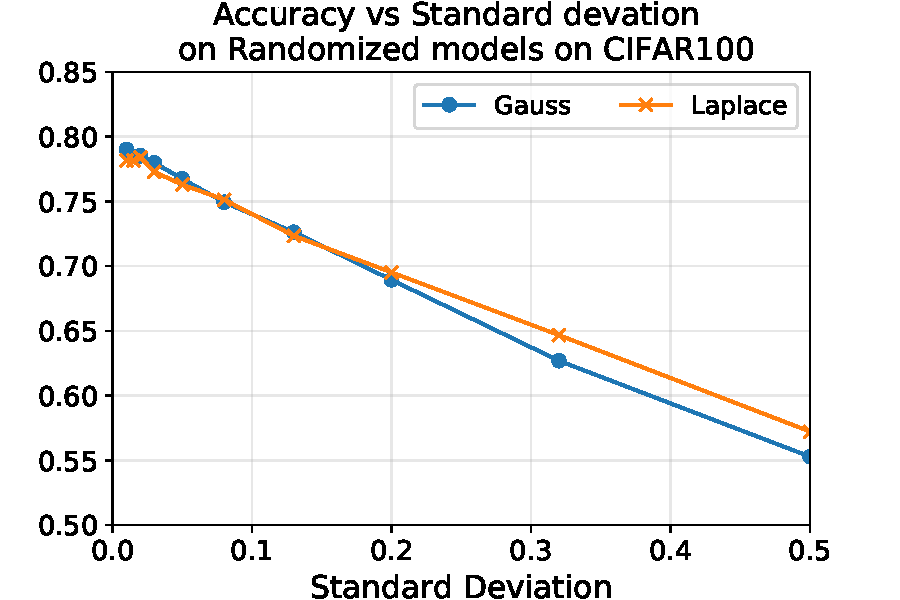
\includegraphics[scale=0.32]{figures/appendix3/acc_sd_CIFAR100.pdf}
    \caption{}
    \label{figure:ap3-acc_sd_CIFAR100-appendix}
  \end{subfigure}
  \begin{subfigure}[t]{0.31\textwidth}
    \centering
    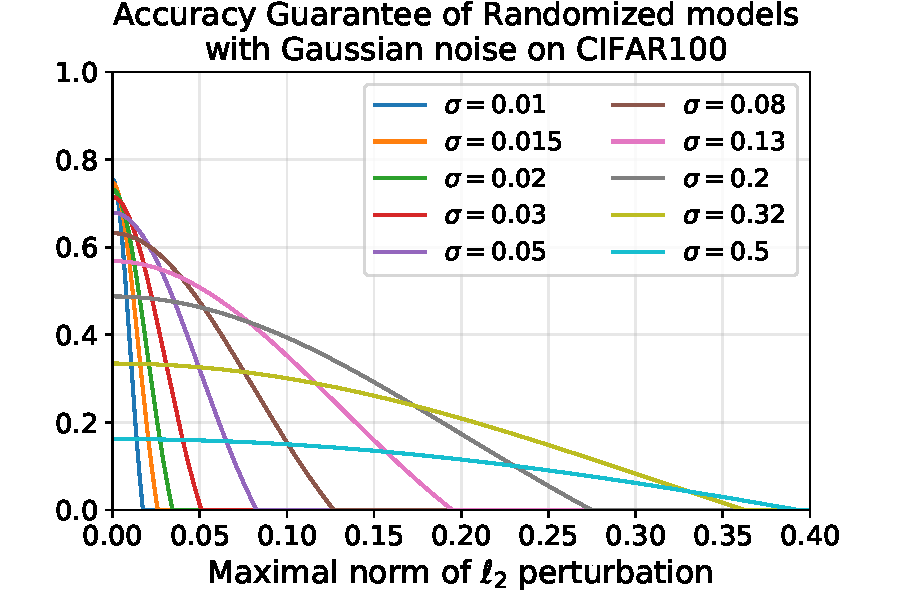
\includegraphics[scale=0.32]{figures/appendix3/gauss_certif_CIFAR100.pdf}
    \caption{}
    \label{figure:ap3-gauss_certif_CIFAR100-appendix}
  \end{subfigure}
  \begin{subfigure}[t]{0.31\textwidth}
    \centering
    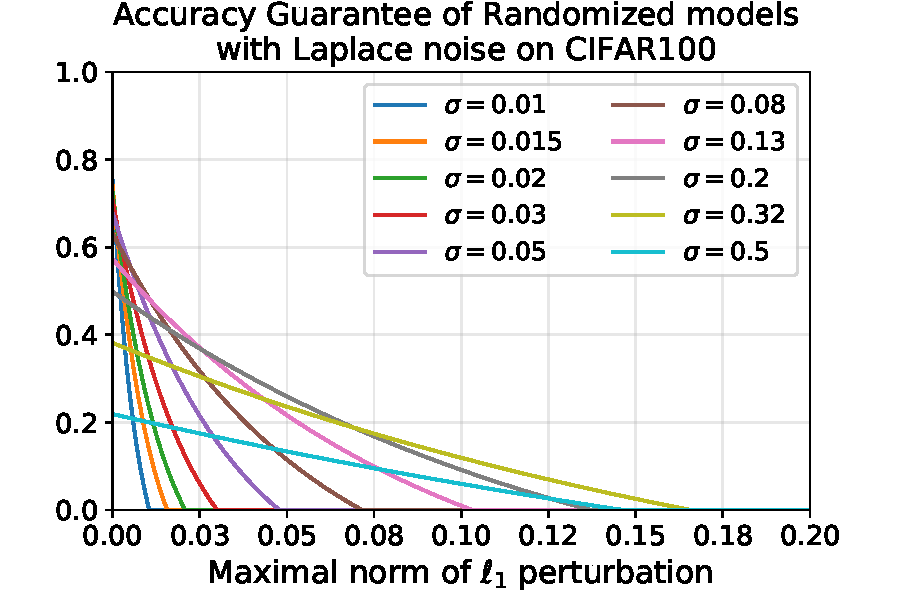
\includegraphics[scale=0.32]{figures/appendix3/laplace_certif_CIFAR100.pdf}
    \caption{}
    \label{figure:ap3-laplace_certif_CIFAR100-appendix}
  \end{subfigure}
  \caption{(a) Impact of the standard deviation of the injected noise on accuracy in a randomized model on CIFAR-100 dataset with a Wide ResNet architecture. (b) and (c) illustration of the guaranteed accuracy of different randomized models with Gaussian (b) and Laplace (c) noises given the norm of the adversarial perturbation.}
\end{figure}

Figure~\ref{figure:ap3-acc_sd_CIFAR100-appendix} presents the trade-off accuracy versus intensity of noise for the CIFAR-100 dataset. As for CIFAR-10, we observe that the accuracy decreases from 0.79 with a small noise (0.01) to $\sim$0.55 with a higher noise (0.5). The Figures~\ref{figure:ap3-gauss_certif_CIFAR100-appendix} and \ref{figure:ap3-laplace_certif_CIFAR100-appendix} are coherent with the theoretical guarantee of accuracy (Theorem~\ref{theorem:ap3-bound-appendix}) that the model can achieve under attack with a given perturbation and noise.   


Table~\ref{table:ap3-cifar10-appendix} and~\ref{table:ap3-cifar100-appendix} summarize the results on the accuracy and accuracy under attack of CIFAR-10 and CIFAR-100 datasets with a Randomized Wide ResNet architecture given the standard deviation of the injected noise and the number of iterations of the attack. For PGD, we use an epsilon max of 0.06 and a step size of 0.006 for an input space of between -1 and +1. We show that injecting noise empirically helps defending neural networks against adversarial attacks.


\begin{table}[htb]
  \centering
  \tiny
  \caption{Accuracy and Accuracy under attack of CIFAR-10 dataset}
  \label{table:ap3-cifar10-appendix}%
    \begin{tabular}{rcccccccccccc}
    \toprule
          & \multirow{2}[3]{*}{\textbf{Natural}} & \multicolumn{3}{c}{\textbf{$\ell_1$ -- EAD}} &       & \multicolumn{3}{c}{\textbf{$\ell_2$ -- C\&W}} &       & \multicolumn{3}{c}{\textbf{$\ell_\infty$ -- PGD}} \\
\cmidrule{3-5}\cmidrule{7-9}\cmidrule{11-13}          &       & \textbf{20} & \textbf{50} & \textbf{60} &       & \textbf{20} & \textbf{50} & \textbf{60} &       & \textbf{10} & \textbf{15} & \textbf{20} \\
    \textbf{Normal (Sd)} &       &       &       &       &       &       &       &       &       &       &       &  \\
    \midrule
    0.010 & 0.954 &       & 0.208 & 0.193 &       & 0.172 & 0.271 & 0.294 &       & 0.411 & 0.428 & 0.408 \\
    0.050 & 0.950 & 0.265 & 0.347 & 0.367 &       & 0.350 & 0.454 & 0.423 &       & 0.638 & 0.549 & 0.486 \\
    0.130 & 0.931 & 0.389 & 0.401 & 0.411 &       & 0.443 & 0.495 & 0.515 &       & 0.710 & 0.636 & 0.553 \\
    0.200 & 0.913 & 0.411 & 0.456 &       &       & 0.470 & 0.481 & 0.516 &       & \textbf{0.724} & 0.629 & 0.539 \\
    0.320 & 0.876 & 0.442 & 0.450 & 0.445 &       & 0.475 & \textbf{0.522} & 0.499 &       & 0.720 & \textbf{0.641} & 0.566 \\
    0.500 & 0.824 & \textbf{0.453} & \textbf{0.513} & \textbf{0.448} &       & \textbf{0.503} & 0.494 & \textbf{0.523} &       & 0.694 & 0.608 & \textbf{0.587} \\
          &       &       &       &       &       &       &       &       &       &       &       &  \\
    \textbf{Laplace (Sd)} &       &       &       &       &       &       &       &       &       &       &       &  \\
    \midrule
    0.010 & 0.955 & 0.167 & 0.190 & 0.208 &       & 0.184 & 0.279 & 0.313 &       & 0.474 & 0.423 & 0.389 \\
    0.050 & 0.950 & 0.326 & 0.315 & 0.355 &       & 0.387 & 0.458 & 0.448 &       & 0.630 & 0.534 & 0.515 \\
    0.130 & 0.929 & 0.388 & 0.426 & 0.435 &       & 0.461 & \textbf{0.515} & 0.493 &       & 0.688 & 0.599 & 0.538 \\
    0.200 & 0.919 & 0.417 &       & \textbf{0.464} &       & 0.484 & 0.481 & 0.501 &       & 0.730 & 0.600 & 0.569 \\
    0.320 & 0.891 & \textbf{0.460} & 0.443 & 0.448 &       & 0.472 & 0.499 & \textbf{0.520} &       & \textbf{0.750} & \textbf{0.665} & 0.576 \\
    0.500 & 0.846 & 0.454 & \textbf{0.471} & \textbf{0.464} &       & \textbf{0.488} &       & 0.494 &       & 0.721 & 0.650 & \textbf{0.589} \\
          &       &       &       &       &       &       &       &       &       &       &       &  \\
    \textbf{Exponential (Sd)} &       &       &       &       &       &       &       &       &       &       &       &  \\
    \midrule
    0.010 & 0.953 & 0.153 & 0.174 &       &       & 0.228 & 0.292 & 0.306 &       & 0.443 & 0.404 & 0.395 \\
    0.050 & 0.953 & 0.312 & 0.326 & 0.330 &       & 0.343 & 0.468 & 0.435 &       & 0.616 & 0.575 & 0.479 \\
    0.130 & 0.940 & 0.373 & 0.402 & 0.411 &       & 0.424 &       & 0.504 &       & 0.679 & 0.585 & 0.526 \\
    0.200 & 0.936 & 0.394 &       & 0.414 &       & 0.455 & \textbf{0.510} & 0.501 &       & 0.701 & 0.623 & 0.550 \\
    0.320 & 0.919 & \textbf{0.429} & 0.426 & 0.416 &       & \textbf{0.494} & 0.492 & 0.513 &       & 0.739 & 0.638 & 0.564 \\
    0.500 & 0.900 & 0.423 & \textbf{0.454} & \textbf{0.470} &       & 0.488 & 0.494 & \textbf{0.516} &       & \textbf{0.752} & \textbf{0.699} & \textbf{0.594} \\
    \bottomrule
    \end{tabular}%
\end{table}%


\begin{table}[htbp]
  \centering
  \tiny
  \caption{Accuracy and Accuracy under attack of CIFAR-100 dataset.}
  \label{table:ap3-cifar100-appendix}%
    \begin{tabular}{rcccccccccccc}
    \toprule
          & \multirow{2}[3]{*}{\textbf{Natural}} & \multicolumn{3}{c}{\textbf{$\ell_1$ -- EAD}} &       & \multicolumn{3}{c}{\textbf{$\ell_2$ -- C\&W}} &       & \multicolumn{3}{c}{\textbf{$\ell_\infty$ -- PGD}} \\
\cmidrule{3-5}\cmidrule{7-9}\cmidrule{11-13}          &       & \textbf{20} & \textbf{50} & \textbf{60} &       & \textbf{20} & \textbf{50} & \textbf{60} &       & \textbf{10} & \textbf{15} & \textbf{20} \\
    \textbf{Normal (Sd)} &       &       &       &       &       &       &       &       &       &       &       &  \\
    0.010 & 0.790 & 0.235 & 0.234 & 0.228 &       & 0.235 & 0.318 & 0.316 &       & 0.257 & 0.176 & 0.187 \\
    0.050 & 0.768 & 0.321 & 0.294 & 0.320 &       & 0.357 & 0.377 & 0.410 &       & 0.377 & 0.296 & 0.254 \\
    0.130 & 0.726 & \textbf{0.357} & \textbf{0.371} & 0.349 &       & 0.387 & \textbf{0.427} & \textbf{0.428} &       & 0.414 & 0.319 & 0.260 \\
    0.200 & 0.689 & 0.338 & 0.350 & \textbf{0.384} &       & 0.394 & 0.381 &       &       & 0.439 & 0.356 & 0.277 \\
    0.320 & 0.627 & 0.334 & 0.344 & 0.350 &       & 0.328 & 0.364 & 0.400 &       & \textbf{0.441} & 0.366 & 0.299 \\
    0.500 & 0.553 & 0.322 & 0.331 & 0.331 &       & 0.349 & 0.342 & 0.351 &       & 0.408 & \textbf{0.374} & \textbf{0.308} \\
          &       &       &       &       &       &       &       &       &       &       &       &  \\
    \textbf{Laplace (Sd)} &       &       &       &       &       &       &       &       &       &       &       &  \\
    \midrule
    0.010 & 0.782 & 0.199 & 0.227 & 0.243 &       & 0.225 & 0.311 & 0.321 &       & 0.236 & 0.190 & 0.177 \\
    0.050 & 0.763 & 0.326 & 0.317 & 0.331 &       & 0.354 & 0.377 & 0.409 &       & 0.368 & 0.319 & 0.256 \\
    0.130 & 0.723 & 0.337 & 0.357 & 0.344 &       & \textbf{0.408} & 0.414 & 0.408 &       & 0.420 & 0.346 & 0.293 \\
    0.200 & 0.695 & \textbf{0.355} & 0.349 & \textbf{0.361} &       & 0.393 & 0.405 & 0.393 &       & 0.445 & 0.340 & 0.303 \\
    0.320 & 0.647 & 0.324 & \textbf{0.373} & 0.357 &       & 0.388 & 0.387 & 0.373 &       & \textbf{0.460} & 0.381 & 0.303 \\
    0.500 & 0.572 & 0.310 & 0.308 & 0.323 &       & 0.358 & 0.351 & 0.361 &       & 0.425 & \textbf{0.403} & \textbf{0.329} \\
          &       &       &       &       &       &       &       &       &       &       &       &  \\
    \textbf{Exponential (Sd)} &       &       &       &       &       &       &       &       &       &       &       &  \\
    \midrule
    0.010 & 0.785 & 0.218 & 0.251 & 0.217 &       & 0.247 & 0.278 & 0.321 &       & 0.250 & 0.214 & 0.169 \\
    0.050 & 0.767 & 0.323 & 0.337 & 0.317 &       & 0.346 & 0.380 & 0.402 &       & 0.356 & 0.291 & 0.235 \\
    0.130 & 0.749 & 0.330 &       & 0.356 &       & \textbf{0.403} & \textbf{0.444} & \textbf{0.421} &       & 0.400 & 0.328 & 0.266 \\
    0.200 & 0.731 & 0.345 & 0.361 & 0.357 &       & 0.388 & 0.424 & 0.406 &       & 0.427 & 0.340 & 0.267 \\
    0.320 & 0.703 & 0.349 & 0.351 & 0.340 &       & 0.388 & 0.439 & 0.399 &       & 0.433 & 0.351 & 0.280 \\
    0.500 & 0.673 & \textbf{0.387} & \textbf{0.378} & \textbf{0.378} &       & 0.396 & 0.435 &       &       & \textbf{0.485} & \textbf{0.370} & \textbf{0.322} \\
    \bottomrule
    \end{tabular}%
\end{table}%

%%%%%%%%%%%%%%%%%%%%%%%%%%%%%%%%%%%%%%%%%%%%%%%%%%%%%%%%%%%%%%%%%%%%%%%%%%%%%%%
\subsection{Large scale robustness}
%%%%%%%%%%%%%%%%%%%%%%%%%%%%%%%%%%%%%%%%%%%%%%%%%%%%%%%%%%%%%%%%%%%%%%%%%%%%%%%

Adversarial training fails to generalize to higher dimensional datasets such as ImageNet.
We conducted experiments with the large scale ImageNet dataset and compared our randomized neural network against large scale adversarial training proposed by~\citet{kurakin2016adversarial}.
One can observe from Table~\ref{table:ap3-adv_imagenet-appendix} that the model from ~\citet{kurakin2016adversarial} is neither robust against recent $\ell_1$ nor $\ell_2$ iterative attacks such as EAD and C\&W.
Moreover, it offers a small robustness against $\ell_\infty$ PGD attack.
Our randomized neural network with $\EoT$ attacks offers a small robustness on $\ell_1$ and $\ell_2$ attacks while being less robust against PGD. 

\begin{table}[htb]
  \centering
  \caption{Accuracy under attack of the Adversarial model training by \citet{kurakin2016adversarial} and an Inception Resnet v2 model training with normal 0.1 noise injected in the image on the ImageNet dataset.}
  \label{table:ap3-adv_imagenet-appendix}
  \centering
  \begin{tabular}{lcccccc}
    \toprule
      & \textbf{Baseline} & \textbf{$\ell_1$ EAD 60} & \textbf{$\ell_2$ C\&W 60} & \textbf{$\ell_\infty$ PGD} \\
    \midrule
    \textbf{Kurakin et al. \cite{kurakin2016adversarial}} & 0.739 & 0.097 & 0.100 & 0.239 \\
    \textbf{Normal 0.1} & 0.625 & 0.255 & 0.301 & 0.061 \\
    \bottomrule
  \end{tabular}
\end{table}

%%%%%%%%%%%%%%%%%%%%%%%%%%%%%%%%%%%%%%%%%%%%%%%%%%%%%%%%%%%%%%%%%%%%%%%%%%%%%%%
\subsection{Experiments with noise on the first activation}
%%%%%%%%%%%%%%%%%%%%%%%%%%%%%%%%%%%%%%%%%%%%%%%%%%%%%%%%%%%%%%%%%%%%%%%%%%%%%%%

The aim of the following experiments is empirically illustrate the \textit{Data processing inequality} in Proposition~\ref{propsition:ap3-:postprocessing-appendix}. 

Table~\ref{table:ap3-acc_noise_activation-appendix} and \ref{table:ap3-attack_noise_activation-appendix} present the experiments conducted with the same set of parameters as the previous ones  on CIFAR-10 and CIFAR-100, but with the noise injected in the first activation layer instead of directly in the image. We observe from  Table~\ref{table:ap3-acc_noise_activation-appendix} that we can inject more noise with a marginal loss on accuracy. The accuracy under attack is presented in Table \ref{table:ap3-attack_noise_activation-appendix} for a selection of models. 

\begin{table}[htbp]
  \centering
  \caption{Impact of the distribution and the intensity of the noise with randomized networks with noise injected on the first activation}
  \label{table:ap3-acc_noise_activation-appendix}%
    \begin{tabular}{rcrrcrrc}
    \toprule
    \multicolumn{1}{c}{\textbf{Sd}} & \textbf{Normal} &       & \multicolumn{1}{c}{\textbf{Sd}} & \textbf{Laplace} &       & \multicolumn{1}{c}{\textbf{Sd}} & \textbf{Exponential} \\
    \cmidrule{1-2}\cmidrule{4-5}\cmidrule{7-8}    0.01  & 0.956 &       & 0.01  & 0.955 &       & 0.01  & 0.953 \\
    0.23  & 0.943 &       & 0.05  & 0.947 &       & 0.08  & 0.943 \\
    0.45  & 0.935 &       & 0.10  & 0.933 &       & 0.15  & 0.938 \\
    0.68  & 0.926 &       & 0.15  & 0.916 &       & 0.23  & 0.925 \\
    0.90  & 0.916 &       & 0.20  & 0.911 &       & 0.30  & 0.919 \\
    1.00  & 0.916 &       & 0.25  & 0.897 &       & 0.38  & 0.903 \\
    1.34  & 0.906 &       & 0.30  & 0.889 &       & 0.45  & 0.897 \\
    1.55  & 0.900 &       & 0.35  & 0.882 &       & 0.53  & 0.886 \\
    1.77  & 0.893 &       & 0.40  & 0.867 &       & 0.60  & 0.885 \\
    2.00  & 0.886 &       & 0.45  & 0.855 &       & 0.68  & 0.875 \\
    \bottomrule
    \end{tabular}%
\end{table}%


\begin{table}[htbp]
  \caption{Accuracy and Accuracy under attack of selected models with noise on the first activation}
   \label{table:ap3-attack_noise_activation-appendix}%
    \begin{tabular}{llcccccccccccc}
    \toprule
      & & & \multirow{2}[3]{*}{\textbf{Natural}} & \multicolumn{3}{c}{\textbf{$\ell_1$ -- EAD}} & & \multicolumn{3}{c}{\textbf{$\ell_2$ -- C\&W}} & & \multicolumn{2}{c}{\textbf{$\ell_\infty$ -- PGD}} \\
      \cmidrule{5-7}\cmidrule{9-11}\cmidrule{13-14} & & & & \textbf{20} & \textbf{50} & \textbf{60} & & \textbf{20} & \textbf{50} & \textbf{60} &       & \textbf{10} & \textbf{20} \\
      \textbf{Dataset} & \multicolumn{1}{c}{\textbf{Distribution}} & \textbf{Sd} & & & & & & & & & & &  \\
    \midrule
    \multirow{3}[1]{*}{CIFAR10} & Normal & 1.55  & 0.900 & 0.441 & 0.440 & 0.413 & & 0.477 & 0.482 & 0.484 & & 0.683 & 0.526 \\
     & Laplace & 0.25  & 0.897 & 0.388 & 0.436 & \textbf{0.445} & & 0.481 & 0.506 & 0.491 & & 0.664 & 0.493 \\
     & Exponential & 0.38  & \textbf{0.903} & \textbf{0.456} & \textbf{0.463} & 0.438 & & \textbf{0.495} & \textbf{0.516} & \textbf{0.506} &       & \textbf{0.697} & \textbf{0.557} \\
    \midrule
    \multirow{3}[2]{*}{CIFAR100} & Normal & 0.45  & 0.741 & \textbf{0.362} & 0.352 & 0.353 & & 0.352 & 0.410 & 0.418 & & 0.380 & 0.250 \\
     & Laplace & 0.10  & \textbf{0.742} & 0.350 & \textbf{0.367} & 0.350 & & 0.371 & \textbf{0.419} & & & 0.418 & \textbf{0.264} \\
     & Exponential & 0.15  & 0.741 & 0.354 & 0.356 & \textbf{0.373} & & \textbf{0.394} & 0.409 & \textbf{0.420} & & \textbf{0.430} & 0.258 \\
    \bottomrule
    \end{tabular}%
\end{table}%



%%%%%%%%%%%%%%%%%%%%%%%%%%%%%%%%%%%%%%%%%%%%%%%%%%%%%%%%%%%%%%%%%%%%%%%%%%%%%%%
\section{Additional discussions on the experiments}
%%%%%%%%%%%%%%%%%%%%%%%%%%%%%%%%%%%%%%%%%%%%%%%%%%%%%%%%%%%%%%%%%%%%%%%%%%%%%%%

For the sake of completeness and reproducibility, we give some additional insights on the noise injection scheme and comprehensive details on our numerical experiments.

%%%%%%%%%%%%%%%%%%%%%%%%%%%%%%%%%%%%%%%%%%%%%%%%%%%%%%%%%%%%%%%%%%%%%%%%%%%%%%%
\subsection{On the need for injecting noise in the training phase}
\label{section:ap3-covariateshift-appendix}
%%%%%%%%%%%%%%%%%%%%%%%%%%%%%%%%%%%%%%%%%%%%%%%%%%%%%%%%%%%%%%%%%%%%%%%%%%%%%%%

Robustness has always been thought as a property to be enforced at inference time and it is tempting to focus only on injecting noise at inference.
However, simply doing so ruins the accuracy of the algorithm (as it becomes an instance of distribution shift~\cite{sugiyama2012machine}).
Indeed, making the assumption that the training and test distributions matches, in practice, injecting some noise at inference would result in changing the test distribution.

Distribution shift occurs when the training distribution differs from the test distribution.
This implies that the hypothesis minimizing the empirical risk is not consistent, \ie, it does not converge to the true model as the training size increases.
A way to circumvent that is to ensure that training and test distributions matches using importance weighting (in the case of covariate-shift) or with noise injection in the training phases as well (in our case).


%%%%%%%%%%%%%%%%%%%%%%%%%%%%%%%%%%%%%%%%%%%%%%%%%%%%%%%%%%%%%%%%%%%%%%%%%%%%%%%
\subsection{Reproducibility of the  experiments}
%%%%%%%%%%%%%%%%%%%%%%%%%%%%%%%%%%%%%%%%%%%%%%%%%%%%%%%%%%%%%%%%%%%%%%%%%%%%%%%

We emphasize that all experiments should be easily reproducible.
All our experiments are developed with TensorFlow version 1.12~\cite{tensorflow2015-whitepaper}.
The code is available as supplemental material and will be open sourced upon acceptance of the paper.
The archive contains a \emph{readme} file containing a small documentation on how to run the experiments, a configuration file which defines the architecture and the hyper-parameters of the experiments, python scripts which generate a bash command to run the experiments.
The code contains Randomized Wide Resnet used for CIFAR-10 and CIFAR100, Inception Resnet v2 used for ImageNet, PGD, EAD and C\&W attacks used for evaluation under attack.
We ran our experiments, on a cluster with computers each having 8 GPU Nvidia V100. 









    %%%%%%%%%%%%%%%%%%%%%%%%%%%%%%%%%%%%%%%%%%%%%%%%%%%%%%%%%%%%%%%%%%%%%%%%%%%%%%%
\chapter{Advocating for Multiple Defense Strategies against Adversarial Examples}
\label{chapter:advocating_multiple_defense_strategies_against_adversarial_examples}
%%%%%%%%%%%%%%%%%%%%%%%%%%%%%%%%%%%%%%%%%%%%%%%%%%%%%%%%%%%%%%%%%%%%%%%%%%%%%%%
\localtableofcontents

% \begin{abstract}
%   It has been empirically observed that defense mechanisms designed to protect neural networks against $\linf$ adversarial examples offer poor performance against $\ltwo$ adversarial examples and vice versa. In this paper we conduct a geometrical analysis that validates this observation. Then, we provide a number of empirical insights to illustrate the effect of this phenomenon in practice. 
%   Then, we review some of the existing defense mechanism that attempts to defend against multiple attacks by mixing defense strategies. Thanks to our numerical experiments, we discuss the relevance of this method and state open questions for the adversarial examples community.
% \end{abstract}

\emph{This Appendix concerns a collaboration ..}

\todo{write short context}


%%%%%%%%%%%%%%%%%%%%%%%%%%%%%%%%%%%%%%%%%%%%%%%%%%%%%%%%%%%%%%%%%%%%%%%%%%%%%%%
\section{Introduction}
\label{section:ap4-introduction}
%%%%%%%%%%%%%%%%%%%%%%%%%%%%%%%%%%%%%%%%%%%%%%%%%%%%%%%%%%%%%%%%%%%%%%%%%%%%%%%

Deep neural networks achieve state-of-the-art performances in a variety of domains such as natural language processing~\cite{radford2018Language}, image recognition~\cite{He_2016_CVPR} and speech recognition~\cite{hinton2012deep}.
However, it has been shown that such neural networks are vulnerable to \emph{adversarial examples}, \ie, imperceptible variations of the natural examples, crafted to deliberately mislead the models~\cite{globerson2006nightmare,biggio2013evasion,Szegedy2013IntriguingPO}.
Since their discovery, a variety of algorithms have been developed to generate adversarial examples (\aka attacks), for example FGSM \cite{goodfellow2014explaining}, PGD \cite{madry2018towards} and C\&W \cite{carlini2017towards}, to mention the most popular ones.

Because it is difficult to characterize the space of visually imperceptible variations of a natural image, existing adversarial attacks use surrogates that can differ from one attack to another.
For example, \citet{goodfellow2014explaining} use the $\linf$ norm to measure the distance between the original image and the adversarial image whereas \citet{carlini2017towards} use the $\ltwo$ norm.
When the input dimension is low, the choice of the norm is of little importance because the $\linf$ and $\ltwo$ balls overlap by a large margin, and the adversarial examples lie in the same space.
An important insight in this paper is to observe that the overlap between the two balls  diminishes exponentially quickly as the dimensionality of the input space increases.
For typical image datasets with large dimensionality, the two balls are mostly disjoint.
As a consequence, the $\linf$ and the $\ltwo$ adversarial examples lie in different areas of the space, and it explains why $\linf$ defense mechanisms perform poorly against $\ltwo$ attacks and vice versa. 

Building on this insight, we advocate for designing models that incorporate defense mechanisms against both $\linf$ and $\ltwo$ attacks and review several ways of mixing existing defense mechanisms.
In particular, we evaluate the performance of  {\em Mixed Adversarial Training} (MAT)~\cite{goodfellow2014explaining} which consists of  augmenting training batches using \emph{both} $\linf$ and $\ltwo$ adversarial examples, and {\em Randomized Adversarial Training} (RAT)~\cite{salman2019provably}, a solution to benefit from the advantages of both $\linf$ adversarial training, and $\ltwo$ randomized defense. 


% \paragraph{Outline of the chapter.}
% The rest of this paper is organized as follows.
% In Section~\ref{section:ap4-preliminaries}, we recall the principle of existing attacks and defense mechanisms.
% In Section~\ref{section:ap4-no_free_lunch}, we conduct a theoretical analysis to show why  the $\linf$ defense mechanisms cannot be robust against $\ltwo$ attacks and vice versa.
% We then corroborate this analysis with empirical results using real adversarial attacks and defense mechanisms.
% In Section~\ref{section:ap4-reviewing_defenses_against_multiple_attacks}, we discuss various strategies to mix defense mechanisms, conduct comparative experiments, and discuss the performance of each strategy.


%%%%%%%%%%%%%%%%%%%%%%%%%%%%%%%%%%%%%%%%%%%%%%%%%%%%%%%%%%%%%%%%%%%%%%%%%%%%%%%
\section{Preliminaries on Adversarial Attacks and Defenses}
\label{section:ap4-preliminaries}
%%%%%%%%%%%%%%%%%%%%%%%%%%%%%%%%%%%%%%%%%%%%%%%%%%%%%%%%%%%%%%%%%%%%%%%%%%%%%%%

Let us first consider a standard classification task with an input space $\mathcal{X}=[0,1]^d$ of dimension $d$,  an output space $\mathcal{Y}=[K]$ and a data distribution $\mathcal D$ over $\mathcal X \times \mathcal Y$.
We assume the model $f_\theta$ has been trained to minimize the expectation over $\mathcal{D}$ of a loss function $\mathcal{L}$ as follows:
\begin{equation}
  \min_{\theta} \Ebb_{(\xvec, y) \sim \mathcal{D}} \left[ \mathcal{L}(f_\theta(\xvec), y) \right]. 
  \label{eqn:classification}
\end{equation}

%%%%%%%%%%%%%%%%%%%%%%%%%%%%%%%%%%%%%%%%%%%%%%%%%%%%%%%%%%%%%%%%%%%%%%%%%%%%%%%
\subsection{Adversarial attacks}
\label{subsection:ap4-adversarial_attacks}
%%%%%%%%%%%%%%%%%%%%%%%%%%%%%%%%%%%%%%%%%%%%%%%%%%%%%%%%%%%%%%%%%%%%%%%%%%%%%%%
 
Given an input-output pair $(\xvec, y) \sim \mathcal{D}$, an \emph{adversarial attack} is a procedure that produces a small perturbation $\tau \in  \mathcal X$  such that $f_\theta(\xvec + \tau) \neq y$.
To find the best perturbation $\tau$, existing attacks can adopt one of the two following strategies:
\begin{itemize}
  \item[(i)] \textbf{Loss maximization}: maximizing the loss $\mathcal L(f_\theta(\xvec + \tau), y)$ under some constraint on $\norm{\tau}_p$ with $p \in \{0, \cdots, \infty\}$.;
  \item[(ii)] \textbf{perturbation minimization}: minimizing $\norm{\tau}_p$ under some constraint on the loss $\mathcal{L}(f_\theta(\xvec + \tau), y)$.
\end{itemize}

\paragraph{(i) Loss maximization.}
In this scenario, the procedure maximizes the loss objective function, under the constraint that the $\lp$ norm of the perturbation remains bounded by some value $\epsilon$, as follows:  

\begin{equation}
  \argmax_{\norm{\tau}_p \leq \epsilon} \mathcal{L}(f_\theta(\xvec + \tau),y).
  \label{equation:ap4-lossmax}
\end{equation}

The typical value of $\epsilon$ depends on the norm $\norm{/ \cdot\ }_p$ considered in the problem setting.
In order to compare $\linf$ and $\ltwo$ attacks of similar strength, we choose values of $\epsilon_\infty$ and $\epsilon_2$ (for $\linf$ and $\ltwo$ norms respectively) which result in $\linf$ and $\ltwo$ balls of equivalent volumes.
For the particular case of CIFAR-10, this would lead us to choose $\epsilon_\infty = 0.03$ and $\epsilon_2 = 0.8$ which correspond to the maximum values chosen empirically to avoid the generation of visually detectable perturbations. 
The current state-of-the-art method to solve Problem~(\ref{equation:ap4-lossmax}) is based on a projected gradient descent (PGD)~\cite{madry2018towards} of radius~$\epsilon$. Given a budget $\epsilon$, it recursively computes
\begin{equation}
    \xvec^{t+1}=\prod_{B_p(\xvec,\epsilon)}\left(\xvec^t
    +\alpha \argmax_{\delta \text{ s.t. } \norm{\delta}_p \leq 1} \left( \Delta^t \ |\ \delta \right)\right)
    \label{eq:projectionPGD}
\end{equation}
where $B_p(\xvec,\epsilon) = \{ \xvec + \tau \text{ s.t. } \norm{\tau}_p \leq \epsilon\}$, $\Delta^t = \nabla_\xvec \mathcal{L}\left( f_\theta \left(\xvec^t \right), y \right)$, $\alpha$ is a gradient step size, and $\prod_S$ is the projection operator on $S$. Both PGD attacks with $p=2$, and $p=\infty$ are currently used in the literature as state-of-the-art attacks for the loss maximization problem. 


\paragraph{(ii) Perturbation minimization.}
This type of procedure search for the perturbation that has the minimal $\lp$ norm, under the constraint that $\mathcal{L}(f_\theta(\xvec + \tau), y)$ is bigger than a given bound $c$:
\begin{equation}
  \argmin_{\mathcal{L}(f_\theta(\xvec + \tau), y) \geq c} \norm{\tau}_p.
  \label{equation:ap4-normmin}
\end{equation}
The value of $c$ is typically chosen depending on the loss function $\mathcal{L}$. For example, if $\mathcal{L}$ is the $0/1$ loss, any $c > 0$ is acceptable.
Problem~\ref{equation:ap4-normmin} has been tackled by~\citep{carlini2017towards}, leading to the following method, denoted C\&W attack in the rest of the chapter. It aims at solving the following Lagrangian relaxation of Problem~\ref{equation:ap4-normmin}:
\begin{equation}
  \argmin_{\tau} \norm{\tau}_p+ \lambda \times g(x+\tau)
  \label{eq:CWproblem}
\end{equation}
where $g(x+\tau)<0$ if and only if $\mathcal{L}(f_\theta(x+\tau),y) \geq c$. 
The authors use a change of variable $\tau=\tanh(w)-x$ to ensure that $-1 \leq x+\tau \leq 1$, a binary search to optimize the constant $c$, and Adam or SGD to compute an approximated solution.
The C\&W attack is well defined both for $p=2$, and $p=\infty$, but there is a clear empirical gap of efficiency in favor of the $\ltwo$ attack.

In this paper, we focus on the \emph{Loss Maximization} setting using the PGD attack. However we conduct some of our experiments using \emph{Perturbation Minimization} algorithms such as C\&W to capture more detailed information about the location of adversarial examples in the vector space\footnote{As it has a more flexible geometry than the \emph{Loss Maximization} attacks.}. 

%%%%%%%%%%%%%%%%%%%%%%%%%%%%%%%%%%%%%%%%%%%%%%%%%%%%%%%%%%%%%%%%%%%%%%%%%%%%%%%
\subsection{Defense mechanisms}
\label{subsection:ap4-defense_mechanisms}
%%%%%%%%%%%%%%%%%%%%%%%%%%%%%%%%%%%%%%%%%%%%%%%%%%%%%%%%%%%%%%%%%%%%%%%%%%%%%%%

\paragraph{Adversarial Training (AT).}
\label{paragraph:adversarial_training}

Adversarial Training was introduced by \citep{goodfellow2014explaining} and later improved by \citep{madry2018towards} as a first defense mechanism to train robust neural networks.
It consists in augmenting training batches with adversarial examples generated during the training procedure.
The standard training procedure from Equation~\ref{eqn:classification} is thus replaced by the following  $\min$ $\max$ problem, where the classifier tries to minimize the expected loss under maximum perturbation of its input:
\begin{equation}
  \min_{\theta} \Ebb_{(\xvec, y) \sim \mathcal{D}} \left[ \max_{\norm{\tau}_p \leq \epsilon} \mathcal{L} \left( f_{\theta}(\xvec + \tau), y \right) \right].
\end{equation}

In the case where $p=\infty$, this technique offers good robustness  against $\linf$ attacks \cite{athalye2018obfuscated}. AT can also be used with $\ltwo$ attacks but as we will discuss in Section~\ref{section:ap4-no_free_lunch}, AT with one norm offers poor protection against the other.
The main weakness of Adversarial Training is its lack of formal guarantees.
Despite some recent work providing great insights \cite{sinha2017certifying,zhang2019theoretically}, there is no worst case lower bound yet on the accuracy under attack of this method.


\paragraph{Noise injection mechanisms (NI).}
\label{subsection:ap4-randomized_training}

Another important technique to defend against adversarial examples is to use Noise Injection. 
In contrast with Adversarial Training, Noise Injection mechanisms are usually deployed after training.
In a nutshell, it works as follows.
At inference time, given a unlabeled sample $x$, the network outputs
\begin{equation}
  \tilde{f}_\theta(\xvec) \triangleq f_\theta(\xvec + \eta) \ \ \ (\text{instead of  } f_\theta(\xvec)) 
\end{equation}
where $\eta$ is a random variable on $\mathbb{R}^d$.
Even though, Noise Injection is often less efficient than Adversarial Training in practice (see \eg, Table~\ref{table:ap4-results}), it benefits from strong theoretical background.
In particular, recent works \cite{lecuyer2018certified,NIPS2019_9143}, followed by \cite{KolterRandomizedSmoothing,pinot2019theoretical} demonstrated that noise injection from a Gaussian distribution can give provable defense against $\ltwo$ adversarial attacks.
In this work, besides the classical Gaussian noises already investigated in previous works, we evaluate the efficiency of Uniform distributions to defend against $\ltwo$ adversarial examples. 

%%%%%%%%%%%%%%%%%%%%%%%%%%%%%%%%%%%%%%%%%%%%%%%%%%%%%%%%%%%%%%%%%%%%%%%%%%%%%%%
\section{No Free Lunch for Adversarial Defenses}
\label{section:ap4-no_free_lunch}
%%%%%%%%%%%%%%%%%%%%%%%%%%%%%%%%%%%%%%%%%%%%%%%%%%%%%%%%%%%%%%%%%%%%%%%%%%%%%%%

In this Section, we show both theoretically and empirically that defenses mechanisms intending to defend against $\linf$ attacks cannot provide suitable defense against $\ltwo$ attacks.
Our reasoning is perfectly general; hence we can similarly demonstrate the reciprocal statement, but we focus on this side for simplicity.


\begin{figure}
   \centering
   \begin{subfigure}[b]{0.32\textwidth}
       \centering
       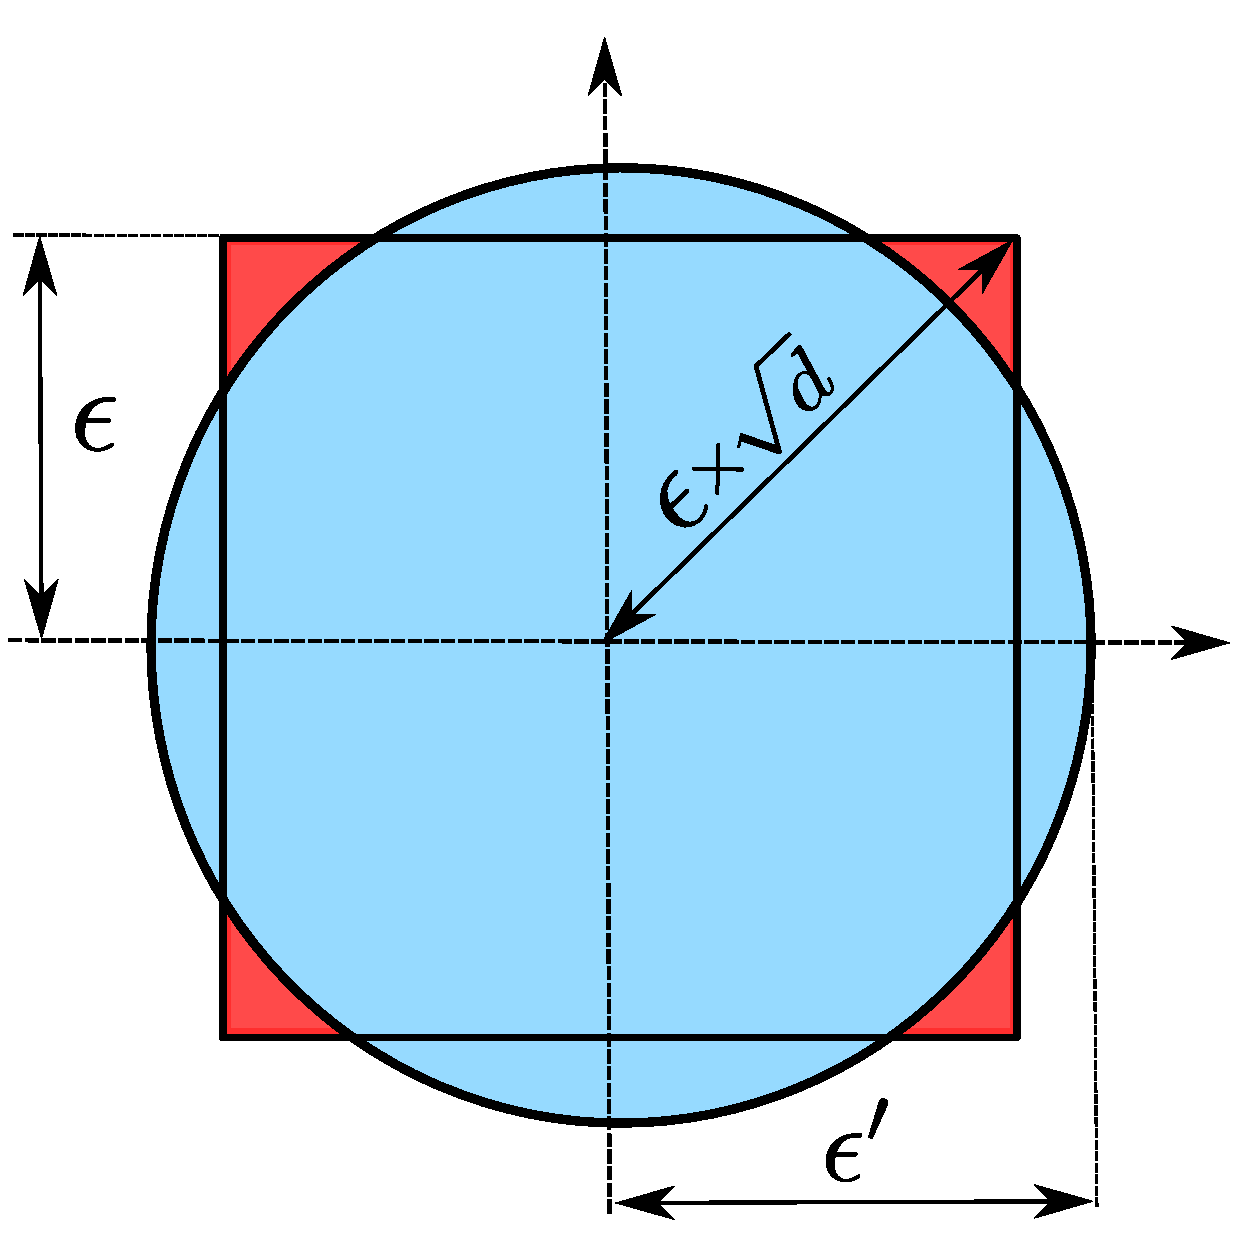
\includegraphics[scale=0.22]{figures/appendix4/ball_inclusion_adversarial_training.pdf}
       \caption{}
       \label{figure:ap4-ball_inclusion_adversarial_training}
   \end{subfigure}
   \hfill
   \begin{subfigure}[b]{0.32\textwidth}
       \centering
       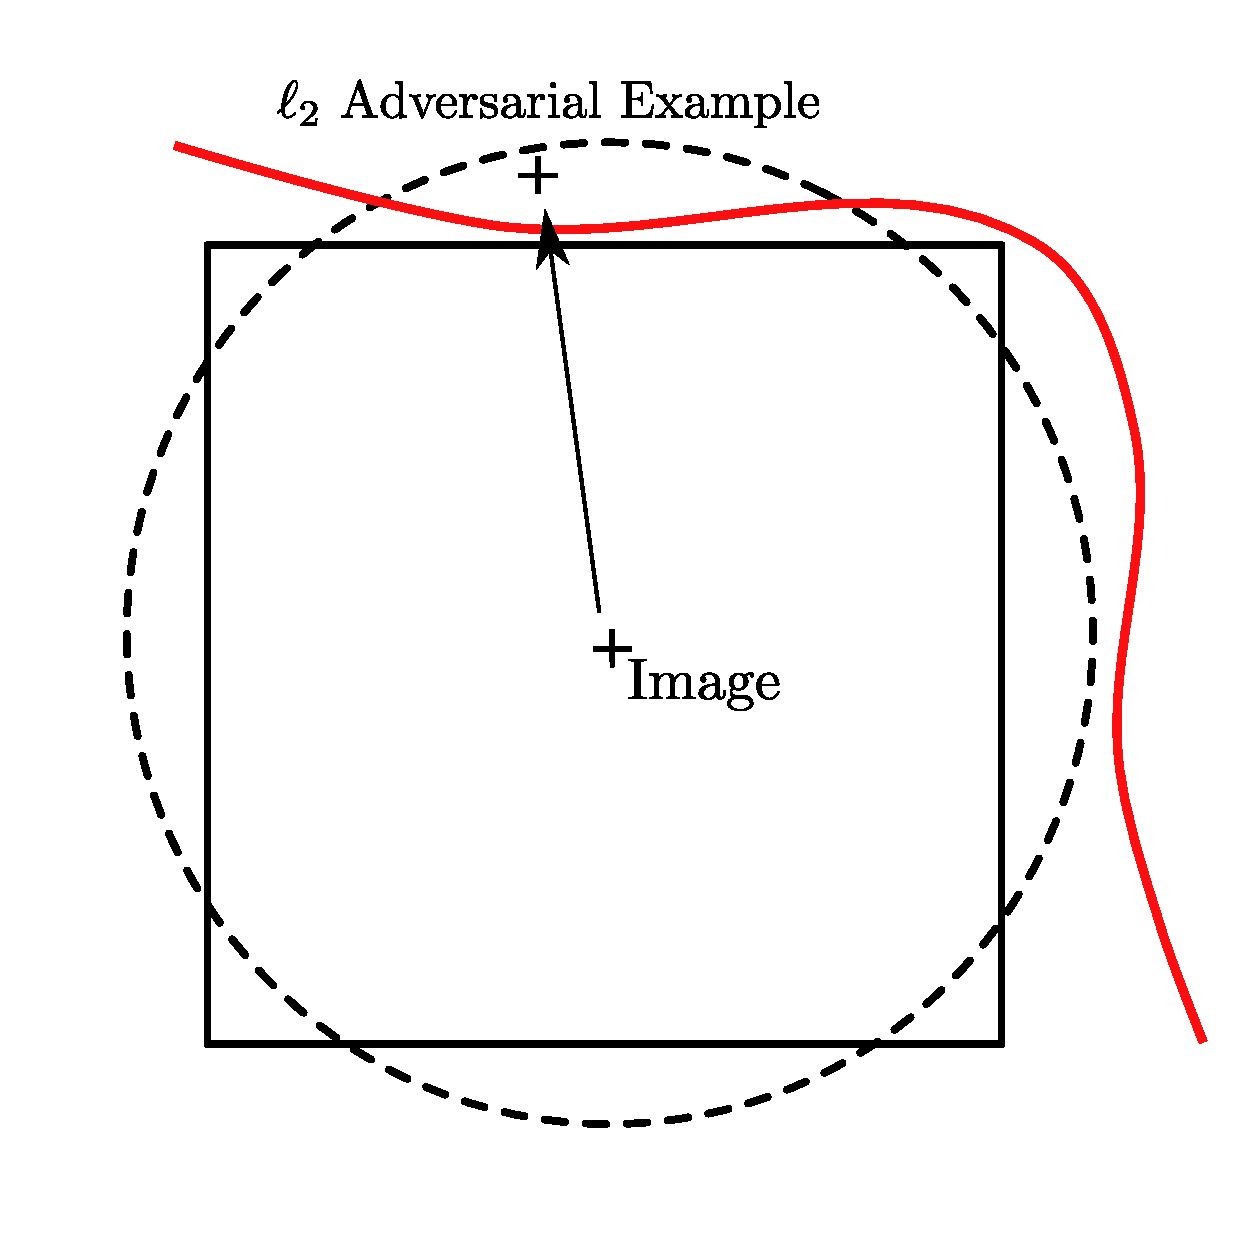
\includegraphics[scale=0.22]{figures/appendix4/ball_adversarial_l2.pdf}
       \caption{}
       \label{figure:ap4-ball_adversarial_l2}
   \end{subfigure}
   \hfill
   \begin{subfigure}[b]{0.32\textwidth}
       \centering
       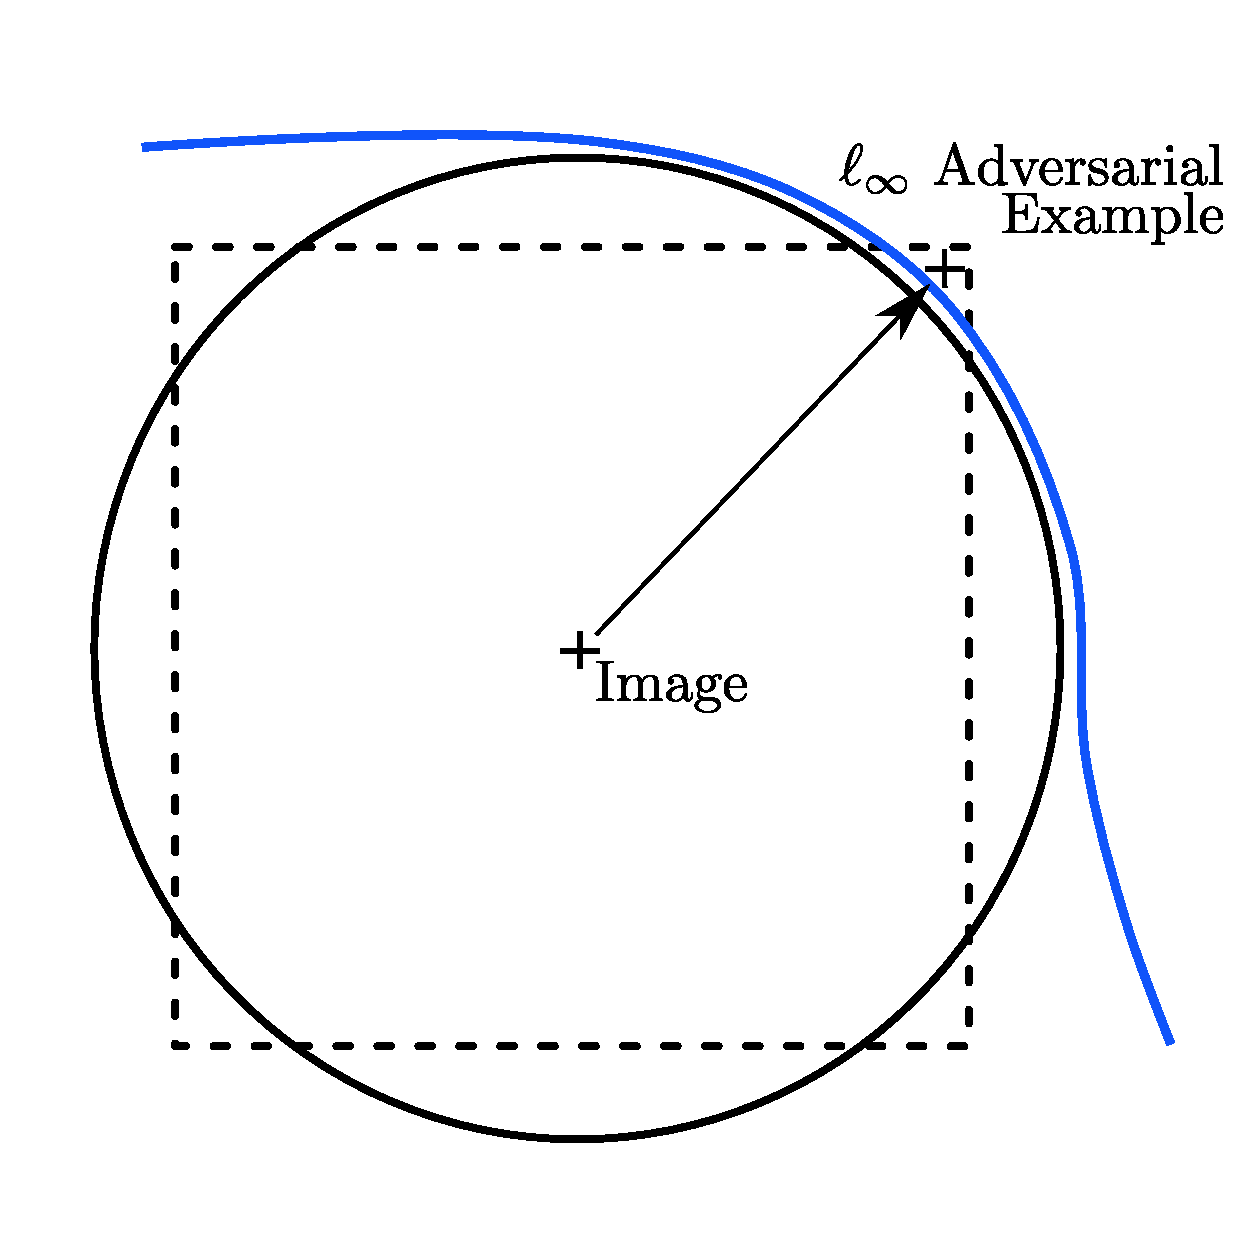
\includegraphics[scale=0.22]{figures/appendix4/ball_adversarial_linf.pdf}
       \caption{}
       \label{figure:ap4-ball_adversarial_linf}
   \end{subfigure}
   \caption{Left: 2D representation of the $\linf$ and $\ltwo$ balls of respective radius $\epsilon$ and $\epsilon'$. 
    Middle: a classifier trained with $\linf$ adversarial perturbations  (materialized by the red line) remains vulnerable to $\ltwo$ attacks. 
    Right: a classifier trained with $\ltwo$ adversarial perturbations (materialized by the blue line) remains vulnerable to $\linf$ attacks.}
\end{figure}


%%%%%%%%%%%%%%%%%%%%%%%%%%%%%%%%%%%%%%%%%%%%%%%%%%%%%%%%%%%%%%%%%%%%%%%%%%%%%%%
\subsection{Theoretical analysis}
\label{subsection:ap4-theoretical_analysis}
%%%%%%%%%%%%%%%%%%%%%%%%%%%%%%%%%%%%%%%%%%%%%%%%%%%%%%%%%%%%%%%%%%%%%%%%%%%%%%%

Let us consider a classifier $f_{\infty}$ that is provably robust against adversarial examples with maximum $\linf$ norm of value $\epsilon_\infty$.
It guarantees that for any input-output pair $(x,y) \sim \mathcal D$ and for any perturbation $\tau$ such that $\norm{\tau}_\infty \leq \epsilon_\infty$, $f_{\infty}$ is not misled by the perturbation, \ie, $f_{\infty}(x + \tau) = f_{\infty}(x)$.
We now focus our study on the performance of this classifier against adversarial examples bounded with a $\ltwo$ norm of value $\epsilon_2$.
Using Figure~\ref{figure:ap4-ball_inclusion_adversarial_training}, we observe that any $\ltwo$ adversarial example that is also in the $\linf$ ball, will not fool $f_{\infty}$.
Conversely, if it is outside the ball, we have no guarantee.

To characterize the probability that such an  $\ltwo$ perturbation fools an $\linf$ defense mechanism in the general case (\emph{i.e.}, any dimension $d$), we measure the ratio between the volume of the intersection of the $\linf$ ball of radius $\epsilon_\infty$ and the $\ltwo$ ball of radius $\epsilon_2$. As Theorem~\ref{theorem:ap4-nullvolume} shows, this ratio depends on the dimensionality $d$ of the input vector $x$, and  rapidly converges to zero when $d$ increases. 
Therefore a defense mechanism that protects against all $\linf$ bounded adversarial examples is unlikely to be efficient against $\ltwo$ attacks. 


\begin{theorem}[Probability of the intersection goes to $0$] ~\\
Let
\begin{equation}
  B_{2,d}(\epsilon) \triangleq \left \{\tau \in \Rbb^d \ |\  \norm{\tau}_2 \leq \epsilon \right \}
\end{equation}
and
\begin{equation}
  B_{\infty,d}(\epsilon') \triangleq \left \{\tau \in \Rbb^d \ |\  \norm{\tau}_\infty \leq \epsilon' \right\}.
\end{equation}
If for all $d$, we select $\epsilon$ and $\epsilon$' such that $\Vol\left(B_{2,d}(\epsilon)\right) = \Vol\left(B_{\infty,d}(\epsilon')\right)$, then
\begin{equation}
  \frac{\Vol\left(B_{2,d}(\epsilon)\bigcap B_{\infty,d}(\epsilon')\right)}{\Vol\left(B_{\infty,d}(\epsilon')\right)} \rightarrow 0 \text{ when } d\rightarrow \infty.
\end{equation}
\label{theorem:ap4-nullvolume}
\end{theorem} 

\begin{proof}[\proofrefth{theorem:ap4-nullvolume}] 
Without loss of generality, let us fix $\epsilon = 1$. One can show that for all $d$, 
\begin{equation}
    \Vol\left( B_{2,d}\left(\frac{2}{\sqrt{\pi}}\Gamma\left(\frac{d}{2}+1\right)^{1/d}\right)\right) = \Vol\left(B_{\infty,d}\left(1\right)\right)
\end{equation}
where $\Gamma$ is the gamma function. Let us denote 
\begin{equation}
    r_2(d)=\frac{2}{\sqrt{\pi}}\Gamma\left(\frac{d}{2}+1\right)^{1/d}.
\end{equation}
Then, thanks to Stirling's formula
\begin{equation}
    r_2(d)\sim \sqrt{\frac{2}{\pi e}} d^{1/2}.
\end{equation}
Finally, if we denote $\mathcal{U}_S$, the uniform distribution on set $S$, by using  Hoeffding inequality between Equation~\ref{equation:ap4-hoeffding1} and \ref{equation:ap4-hoeffding2}, we get:
\begin{align}
  \frac{\Vol(B_{2,d}(r_2(d)) \bigcap B_{\infty,d}(1))}{\Vol(B_{\infty,d}(1))} &= \Pbb_{x \sim \mathcal{U}_{B_{\infty,d}(1)}} \left[ x \in B_{2,d}(r_2(d)) \right] \\
  &= \Pbb_{x \sim \mathcal{U}_{B_{\infty,d}(1)}} \left[ \sum_{i=1}^d |x_i|^2 \leq r_2^2(d) \right] \\
  &\leq \exp{- d^{-1} \left( r_2^2(d) - d \Ebb |x_1|^2 \right)^2} \label{equation:ap4-hoeffding1} \\
  &\leq \exp{-\left( \frac{2}{\pi e}-\frac23\right)^2d+o(d)} \label{equation:ap4-hoeffding2}.
\end{align}
Then the ratio between the volume of the intersection of the ball and the volume of the ball converges towards $0$ when $d$ goes to $\infty$.
\end{proof}

Theorem~\ref{theorem:ap4-nullvolume} states that, when $d$ is large enough, $\ltwo$ bounded perturbations have a null probability of being also in the $\linf$ ball of the same volume.
As a consequence, for any value of $d$ that is large enough, a defense mechanism that offers full protection against $\linf$ adversarial examples is not guaranteed to offer any protection against $\ltwo$ attacks \footnote{Theorem~\ref{theorem:ap4-nullvolume} can easily be extended to any two balls with different norms. For clarity, we restrict to the case of $\linf$ and $\ltwo$ norms.}.

\begin{table}[ht]
  \centering
  \begin{tabular}{c r r r l}
    \toprule
    \textbf{Dataset\ } & \phantom{....} & \textbf{Dim.} $\mathbf{(d)}$ & \phantom{....} & \textbf{Vol. of the intersection }\\
    \midrule
    -- & & 2\ \ & & $10^{-0.009}$ \quad ($\approx$ 0.98) \\
    MNIST & & 784\ \  & & $10^{-144}$\\
    CIFAR & & 3072\ \ & &  $10^{-578}$\\
    ImageNet & & 150528\ \ & & $10^{-28946}$\\
    \bottomrule
  \end{tabular}
  \caption{ Bounds of Theorem~\ref{theorem:ap4-nullvolume} on the volume of the intersection of  $\ltwo$ and $\linf$ balls at equal volume for typical image classification datasets. When $d=2$, the bound is $ 10^{-0.009}\approx 0.98$.}
  \label{table:ap4-datadim}
\end{table}

Note that this result defeats the 2-dimensional intuition: if we consider a 2 dimensional problem setting, the $\linf$ and the $\ltwo$ balls have an important overlap (as illustrated in Figure~\ref{figure:ap4-ball_inclusion_adversarial_training}) and the probability of sampling at the intersection of the two balls is bounded by approximately 98\%.
However, as we increase the dimensionality $d$, this probability quickly becomes negligible, even for very simple image datasets such as MNIST.
An instantiation of  the bound for classical image datasets is presented in Table~\ref{table:ap4-datadim}.
The probability of sampling at the intersection of the $\linf$ and $\ltwo$ balls is close to zero for any realistic image setting.
In large dimensions, the volume of the corner of the $\linf$ ball is much bigger than it appears in Figure~\ref{figure:ap4-ball_inclusion_adversarial_training}.


%%%%%%%%%%%%%%%%%%%%%%%%%%%%%%%%%%%%%%%%%%%%%%%%%%%%%%%%%%%%%%%%%%%%%%%%%%%%%%%
\subsection{No Free Lunch in Practice}
\label{subsection:ap4-no_free_lunch_in_practice}
%%%%%%%%%%%%%%%%%%%%%%%%%%%%%%%%%%%%%%%%%%%%%%%%%%%%%%%%%%%%%%%%%%%%%%%%%%%%%%%

Our theoretical analysis shows that if adversarial examples were uniformly distributed in a high-dimensional space, then any mechanism that perfectly defends against $\linf$ adversarial examples has a null probability of protecting against $\ltwo$-bounded adversarial attacks.
Although existing defense mechanisms do not necessarily assume such a distribution of adversarial examples, we demonstrate that whatever distribution they use, it offers no favorable bias with respect to the result of Theorem~\ref{theorem:ap4-nullvolume}.
As we discussed in Section~\ref{section:ap4-preliminaries}, there are two distinct attack settings: loss maximization (PGD) and perturbation minimization (C\&W).
Our analysis is mainly focusing on loss maximization attacks.
However, these attacks have a very strict geometry\footnote{Due to the projection operator, all PGD attacks saturate the constraint, which makes them all lies in a very small part of the ball.}.
This is why, to present a deeper analysis of the behavior of adversarial attacks and defenses, we also present a set of experiments that use perturbation minimization attacks.

\begin{table}[htbp]
  \centering 
  \begin{tabular}{lrrrrrrrr}
    \toprule
      & \phantom{...}  & \multicolumn{3}{c}{Attack PGD-$\ltwo$} & \phantom{...}  & \multicolumn{3}{c}{Attack PGD-$\linf$} \\
  \cmidrule{3-5}\cmidrule{7-9}      &   & \multicolumn{1}{l}{Unprotected} &  \phantom{...} & \multicolumn{1}{l}{AT-$\linf$} &   & \multicolumn{1}{l}{Unprotected} & \phantom{...}  & \multicolumn{1}{l}{AT-$\ltwo$} \\
    \midrule
    Average $\ltwo$ norm &   & 0.830 &   & 0.830 &   & 1.400 &   & 1.640 \\
    Average $\linf$ norm &   & 0.075 &   & 0.200 &   & 0.031 &   & 0.031 \\
    \bottomrule
  \end{tabular}%
  \caption{Average norms of PGD-$\ltwo$ and PGD-$\linf$ adversarial examples with and without $\linf$ adversarial training on CIFAR-10 ($d=3072$).}
  \label{table:ap4-mean_norm_pgd_attack}
\end{table}%

\paragraph{Adversarial training vs. loss maximization attacks}

To demonstrate that $\linf$ adversarial training is not robust against PGD-$\ltwo$ attacks we measure the evolution of $\ltwo$ norm of adversarial examples generated with PGD-$\linf$ between an unprotected model and a model trained with AT-$\linf$, \ie, AT where adversarial examples are generated with PGD-$\linf$ \footnote{To do so, we use the same experimental setting as in Section~\ref{section:ap4-reviewing_defenses_against_multiple_attacks} with $\epsilon_\infty$ and $\epsilon_2$ such that the volumes of the two balls are equal.}. 
Results are presented in  Table~\ref{table:ap4-mean_norm_pgd_attack}. \footnote{All experiments in this section are conducted on CIFAR-10, and the experimental setting is fully detailed in Section~\ref{section:ap4-experimental_settings}. }

The analysis is unambiguous: the average $\linf$ norm of a bounded $\ltwo$ perturbation more than double between an unprotected model and a model trained with AT PGD-$\linf$. This phenomenon perfectly reflects the illustration of Figure~\ref{figure:ap4-ball_adversarial_linf}. The attack will generate an adversarial example on the corner of the $\linf$ ball thus increasing the $\linf$ norm while maintaining the same $\ltwo$ norm. 
We can observe the same phenomenon with AT-$\ltwo$ against PGD-$\linf$ attack (see Figure~\ref{figure:ap4-ball_adversarial_l2} and Table \ref{table:ap4-mean_norm_pgd_attack}). PGD-$\linf$ attack increases the $\ltwo$ norm while maintaining the same $\linf$ perturbation thus generating the perturbation in the upper area. 

As a consequence, we cannot expect adversarial training $\linf$ to offer any guaranteed protection against $\ltwo$ adversarial examples .

\paragraph{Adversarial training vs. perturbation minimization attacks.}
To better capture the behavior of $\ltwo$ adversarial examples, we now study the performances of an $\ltwo$ perturbation minimization attack (C\&W) with and without AT-$\linf$.
It allows us to understand in which area C\&W discovers adversarial examples and the impact of AT-$\linf$.
In high dimensions, the red corners (see Figure~\ref{figure:ap4-ball_inclusion_adversarial_training}) are very far away from the $\ltwo$ ball.
Therefore, we hypothesize that a large proportion of the $\ltwo$ adversarial examples will remain unprotected.
To validate this assumption, we measure the proportion of adversarial examples inside of the $\ltwo$ ball before and after $\linf$ adversarial training.
The results are presented in Figure~\ref{fig:calotte} (left: without adversarial training, right: with adversarial training). 

\begin{figure}[htb]
    \centering
    \begin{tikzpicture}[scale=0.7]
    \begin{groupplot}[group style={
                        group name=myplot,
			group size= 2 by 1,
		        horizontal sep=3cm},
                      grid style=dashed,
		      ymajorgrids=true]
       
    \nextgroupplot[
       stack plots=y,
       area style,
       ytick={0,5000,1000},
       ymin=0,
       ymax=10000,
       xmin=0.3,
       xmax=16.63,
       axis x line*=bottom,
       axis y line*=left,
       xtick={2,14},
       xticklabels={\Large $\epsilon'=\epsilon\phantom{\sqrt{d}}$, \Large $\epsilon'=\epsilon\times\sqrt{d}$},
       xtick style={draw=none}]
        \addplot table [x=eps,y=linf_ball] {figures/appendix4/data/ball_l2_base.dat}\closedcycle;
        \addplot table [x=eps,y=callote] {figures/appendix4/data/ball_l2_base.dat}\closedcycle;
        \addplot table [x=eps,y=outside] {figures/appendix4/data/ball_l2_base.dat}\closedcycle;

    \nextgroupplot[
       stack plots=y,
       area style,
       ytick={0,5000,1000},
       ymin=0,
       ymax=10000,
       xmin=0.3, 
       xmax=16.63,
       axis x line*=bottom,
       axis y line*=left,
       xtick={2,14},
       xticklabels={\Large $\epsilon'=\epsilon\phantom{\sqrt{d}}$, \Large $\epsilon'=\epsilon\times\sqrt{d}$},
       xtick style={draw=none}]
        \addplot table [x=eps,y=linf_ball] {figures/appendix4/data/ball_l2_at.dat}\closedcycle;
        \addplot table [x=eps,y=callote] {figures/appendix4/data/ball_l2_at.dat}\closedcycle;
        \addplot table [x=eps,y=outside] {figures/appendix4/data/ball_l2_at.dat}\closedcycle;

    \end{groupplot}
\end{tikzpicture}


    \caption{Comparison of the number of adversarial examples found by C\&W, inside the $\linf$ ball (lower, blue area), outside the $\linf$ ball but inside the $\ltwo$ ball (middle, red area) and outside the $\ltwo$ ball (upper gray area). $\epsilon$ is set to $0.3$ and $\epsilon'$ varies along the x-axis. Left: without adversarial training, right: with adversarial training. Most adversarial examples have shifted from the $\linf$ ball to the cap of the $\ltwo$ ball, but remain at the same $\ltwo$ distance from the original example.}
    \label{fig:calotte}
\end{figure}

On both charts, the blue area represents the proportion of adversarial examples that are inside the $\linf$ ball.
The red area represents the adversarial examples that are outside the $\linf$ ball but still inside the $\ltwo$ ball (valid $\ltwo$ adversarial examples).
Finally, the brown-beige area represents the adversarial examples that are beyond the $\ltwo$ bound.
The radius $\epsilon'$ of the $\ltwo$ ball varies along the x-axis from $\epsilon'$ to $\epsilon' \sqrt{d}$.
On the left chart (without adversarial training) most $\ltwo$ adversarial examples generated by C\&W are inside both balls.
On the right chart most of the adversarial examples have been shifted out the $\linf$ ball.
This is the expected consequence of $\linf$ adversarial training.
However, these adversarial examples remain in the $\ltwo$ ball, \ie, they are in the cap of the $\ltwo$ ball.
These examples are equally good from the $\ltwo$ perspective.
This means that even after adversarial training, it is still easy to find good $\ltwo$ adversarial examples, making the $\ltwo$ robustness of AT-$\linf$ almost null. 

%%%%%%%%%%%%%%%%%%%%%%%%%%%%%%%%%%%%%%%%%%%%%%%%%%%%%%%%%%%%%%%%%%%%%%%%%%%%%%%%
\section{Reviewing Defenses Against Multiple Attacks}
\label{section:ap4-reviewing_defenses_against_multiple_attacks}
%%%%%%%%%%%%%%%%%%%%%%%%%%%%%%%%%%%%%%%%%%%%%%%%%%%%%%%%%%%%%%%%%%%%%%%%%%%%%%%%

\begin{table}[htbp]
  \centering
  \begin{tabular}{lccccccccccccccccc}
    \toprule
      &   & \textbf{Baseline} & \phantom{...}  & \multicolumn{2}{c}{\textbf{AT}} & \phantom{...}  & \multicolumn{2}{c}{\textbf{MAT}} &  \phantom{...} & \multicolumn{2}{c}{\textbf{NI}} &  \phantom{...} & \multicolumn{2}{c}{\textbf{RAT}-$\linf$} &  \phantom{...} & \multicolumn{2}{c}{\textbf{RAT}-$\ltwo$} \\
  \cmidrule{3-3}\cmidrule{5-6}\cmidrule{8-9}\cmidrule{11-12}\cmidrule{14-15}\cmidrule{17-18}      &   & -- &   & $\linf$ & $\ltwo$ &   & Max & Rand &   & $\mathcal{N}$ & $\mathcal{U}$ &   & $\mathcal{N}$ & $\mathcal{U}$ &   & $\mathcal{N}$ & $\mathcal{U}$ \\
    \midrule
    Natural &   & 0.94 &   & 0.85 & 0.85 &   & 0.80 & 0.80 &   & 0.79 & 0.87 &   & 0.74 & 0.80 &   & 0.79 & 0.87 \\
    PGD-$\linf$ &   & 0.00 &   & 0.43 & 0.37 &   & 0.37 & 0.40 &   & 0.23 & 0.22 &   & 0.35 & 0.40 &   & 0.23 & 0.22 \\
    PGD-$\ltwo$ &   & 0.00 &   & 0.37 & 0.52 &   & 0.50 & 0.55 &   & 0.34 & 0.36 &   & 0.43 & 0.39 &   & 0.34 & 0.37 \\
    \bottomrule
  \end{tabular}%
  \caption{This table shows a comprehensive list of results consisting of the accuracy of several defense mechanisms against $\ltwo$ and $\linf$ attacks. This table main objective is to compare the overall performance of ‘single‘ norm defense mechanisms (AT and NI presented in the Section~\ref{subsection:ap4-defense_mechanisms}) against mixed norms defense mechanisms (MAT \& RAT mixed defenses presented in Section~\ref{section:ap4-reviewing_defenses_against_multiple_attacks}).}
  \label{table:ap4-results}
\end{table}%

Adversarial attacks have been an active topic in the machine learning community since their discovery~\cite{globerson2006nightmare, biggio2013evasion,Szegedy2013IntriguingPO}.
Many attacks have been developed.
Most of them solve a loss maximization problem with either $\linf$~\cite{goodfellow2014explaining,kurakin2016adversarial,madry2018towards}, $\ltwo$~\cite{carlini2017towards,kurakin2016adversarial,madry2018towards}, $\lone$~\cite{tramer2019adversarial} or $\lzero$~\cite{papernot2016limitations} surrogate norms.
As we showed, these norms are really different in high dimension.
Hence, defending against one norm-based attack is not sufficient to protect against another one. 
In order to solve this problem, we review several strategies to build defenses against multiple adversarial attacks.
These strategies are based on the idea that both types of defense must be used simultaneously in order for the classifier to be protected against multiple attacks.
The detailed description of the experimental setting is described in Section~\ref{section:ap4-experimental_settings}.

%%%%%%%%%%%%%%%%%%%%%%%%%%%%%%%%%%%%%%%%%%%%%%%%%%%%%%%%%%%%%%%%%%%%%%%%%%%%%%%
\subsection{Experimental Setting}
\label{section:ap4-experimental_settings}
%%%%%%%%%%%%%%%%%%%%%%%%%%%%%%%%%%%%%%%%%%%%%%%%%%%%%%%%%%%%%%%%%%%%%%%%%%%%%%%

To compare the robustness provided by the different defense mechanisms, we use strong adversarial attacks and a conservative setting: the attacker has a total knowledge of the parameters of the model (white-box setting) and we only consider untargeted attacks  (a misclassification from one target to any other will be considered as adversarial).
To evaluate defenses based on Noise Injection, we use {\em Expectation Over Transformation} (EOT), the rigorous experimental protocol  proposed by \cite{athalye2017synthesizing} and later used by \cite{athalye2018obfuscated,carlini2019evaluating} to identify flawed defense mechanisms. 

To attack the models, we use state-of-the-art algorithms PGD.
We run PGD with 20 iterations to generate adversarial examples and with 10 iterations when it is used for adversarial training.
The maximum $\linf$ bound is fixed to $0.031$ and the maximum $\ltwo$ bound is fixed to $0.83$.
As discussed in Section~\ref{section:ap4-preliminaries}, we chose these values so that the $\linf$ and the $\ltwo$ balls have similar volumes.
Note that $0.83$ is slightly above the values typically used in previous publications in the area, meaning the attacks are stronger, and thus  more difficult to defend against.

All experiments are conducted on CIFAR-10 with the Wide-Resnet 28-10 architecture.
We use the training procedure and the hyper-parameters described in the original paper by~\cite{ZagoruykoK16}.
Training time varies from 1 day (AT) to 2 days (MAT) on 4 GPUs-V100 servers. 


%%%%%%%%%%%%%%%%%%%%%%%%%%%%%%%%%%%%%%%%%%%%%%%%%%%%%%%%%%%%%%%%%%%%%%%%%%%%%%%
\subsection{MAT -- Mixed Adversarial Training}
\label{subsection:ap4-mixed_adversarial_training}
%%%%%%%%%%%%%%%%%%%%%%%%%%%%%%%%%%%%%%%%%%%%%%%%%%%%%%%%%%%%%%%%%%%%%%%%%%%%%%%

Earlier results have shown that AT-$\lp$ improves the robustness against corresponding $\lp$-bounded adversarial examples, and the experiments we present in this section corroborate this observation (See Table~\ref{table:ap4-results}, column: AT).
Building on this, it is natural to examine the efficiency of \emph{Mixed Adversarial Training} (MAT) against mixed $\linf$ and $\ltwo$ attacks.
MAT is a variation of AT that uses both $\linf$-bounded adversarial examples and $\ltwo$-bounded adversarial examples as training examples.
As discussed in~\cite{tramer2019adversarial}, there are several possible strategies to mix the adversarial training examples.
The first strategy (MAT-Rand) consists in randomly selecting one adversarial example among the two most damaging $\linf$ and $\ltwo$, and to use it as a training example, as described in Equation~(\ref{eq:mat-rand}): 

\paragraph{MAT-Rand}:
\begin{equation}
  \min_{\theta} \Ebb_{(x, y) \sim \mathcal{D}} \left[\Ebb_{p\sim\mathcal{U}({\{2, \infty\})}} \max_{\norm{\tau}_p \leq \epsilon} \mathcal{L} \left( f_{\theta}(x+\tau), y \right) \right].
  \label{eq:mat-rand}
\end{equation}

An alternative strategy is to systematically train the model with the most damaging adversarial example ($\linf$ or $\ltwo$). As described in Equation~(\ref{eq:mat-max}): 

\paragraph{MAT-Max}:
\begin{equation}
    \min_{\theta} \Ebb_{(x, y) \sim \mathcal{D}} \left[ \max_{p \in \{2, \infty\}} \max_{\norm{\tau}_p \leq \epsilon} \mathcal{L} \left( f_{\theta}(x+\tau), y \right) \right].
    \label{eq:mat-max}
\end{equation}

The accuracy of MAT-Rand and MAT-Max are reported in Table~\ref{table:ap4-results} (Column: MAT).
As expected, we observe that MAT-Rand and MAT-Max offer better robustness both against PGD-$\ltwo$ and PGD-$\linf$ adversarial examples than the original AT does.
More  generally, we can see that AT is a good strategy against loss maximization attacks, and thus it is not surprising that MAT is a good strategy against mixed loss maximization attacks.
However efficient in practice, MAT (for the same reasons as AT) lacks theoretical arguments.
In order to get the best of both worlds, \cite{salman2019provably} proposed to mix adversarial training with randomization.  


%%%%%%%%%%%%%%%%%%%%%%%%%%%%%%%%%%%%%%%%%%%%%%%%%%%%%%%%%%%%%%%%%%%%%%%%%%%%%%%
\subsection{RAT -- Randomized Adversarial Training}
\label{subsection:ap4-randomized_adversarial_training}
%%%%%%%%%%%%%%%%%%%%%%%%%%%%%%%%%%%%%%%%%%%%%%%%%%%%%%%%%%%%%%%%%%%%%%%%%%%%%%%

We now examine the performance of Randomized Adversarial Training (RAT) first introduced in~\cite{salman2019provably}.
This technique mixes Adversarial Training with Noise Injection.
The corresponding loss function is defined as follows:
\begin{equation}
  \min_{\theta} \Ebb_{(\xvec, y) \sim \mathcal{D}} \left[ \max_{\norm{\tau}_p \leq \epsilon} \mathcal{L} \left( \tilde{f}_{\theta}(\xvec+\tau), y)  \right) \right].
\end{equation}
where $\tilde{f}_\theta$ is a randomized neural network with noise injection as described in Section~\ref{subsection:ap4-randomized_training}, and $\norm{\ \cdot\ }_p$ define which kind of AT is used.
For each setting, we consider two noise distributions, Gaussian and Uniform as we did with NI.
We also consider two different Adversarial training AT-$\linf$ as well as AT-$\ltwo$. 

The results of RAT are reported in Table~\ref{table:ap4-results}~(Columns: RAT-$\linf$ and RAT-$\ltwo$).
We can observe that RAT-$\linf$ offers the best extra robustness with both noises, which is consistent with previous experiments, since AT is generally more effective against $\linf$ attacks whereas NI is more effective against $\ltwo$-attacks.
Overall, RAT-$\linf$ and a noise from uniform distribution offers the best performances but is still weaker than MAT-Rand.
These results are also consistent with the literature, since adversarial training (and its variants) is the best defense against adversarial examples so far.


%%%%%%%%%%%%%%%%%%%%%%%%%%%%%%%%%%%%%%%%%%%%%%%%%%%%%%%%%%%%%%%%%%%%%%%%%%%%%%%
\section{Conclusion \& Perspective}
%%%%%%%%%%%%%%%%%%%%%%%%%%%%%%%%%%%%%%%%%%%%%%%%%%%%%%%%%%%%%%%%%%%%%%%%%%%%%%%

In this paper, we tackled the problem of protecting neural networks against multiple attacks crafted from different norms.
We demonstrated and gave a geometrical interpretation to explain why most defense mechanisms can only protect against one type of attack.
Then we reviewed existing strategies that mix defense mechanisms in order to build models that are robust against multiple adversarial attacks.
We conduct a rigorous and full comparison of {\em Randomized Adversarial Training} and {\em Mixed Adversarial Training} as defenses against multiple attacks. 

We could argue that both techniques offer benefits and limitations.
We have observed that MAT offers the best empirical robustness against multiples adversarial attacks but this technique is computationally expensive which hinders its use in large-scale applications.
Randomized techniques have the important advantage of providing theoretical guarantees of robustness and being computationally cheaper.
However, the certificate provided by such defenses is still too small for strong attacks.
Furthermore, certain Randomized defenses also suffer from the curse of dimensionality as recently shown by \cite{kumar2020curse}. 

Although, randomized defenses based on noise injection seem limited in terms of accuracy under attack and scalability, they could be improved either by Learning the best distribution to use or by leveraging different types of randomization such as discrete randomization first proposed in \cite{pinot2020randomization}.
We believe that these certified defenses are the best solution to ensure the robustness of classifiers deployed into real-world applications.


    %%%%%%%%%%%%%%%%%%%%%%%%%%%%%%%%%%%%%%%%%%%%%%%%%%%%%%%%%%%%%%%%%%%%%%%%%%%%%%%
\chapter{Datasets}
\label{chapter:datasets}
%%%%%%%%%%%%%%%%%%%%%%%%%%%%%%%%%%%%%%%%%%%%%%%%%%%%%%%%%%%%%%%%%%%%%%%%%%%%%%%

\begin{itemize}
  \item MNIST
  \item CIFAR10/100
  \item ImageNet
  \item Youtube-8M
\end{itemize}

\todo{Complete appendix dataset}

    %%%%%%%%%%%%%%%%%%%%%%%%%%%%%%%%%%%%%%%%%%%%%%%%%%%%%%%%%%%%%%%%%%%%%%%%%%%%%%%
\chapter{Publications}
\label{chapter:publications}
%%%%%%%%%%%%%%%%%%%%%%%%%%%%%%%%%%%%%%%%%%%%%%%%%%%%%%%%%%%%%%%%%%%%%%%%%%%%%%%

\todo{Make list of publications}

  \end{appendices} 

  \printbibliography[title=References]


\end{document}
